\documentclass[twoside]{book}

% Packages required by doxygen
\usepackage{fixltx2e}
\usepackage{calc}
\usepackage{doxygen}
\usepackage[export]{adjustbox} % also loads graphicx
\usepackage{graphicx}
\usepackage[utf8]{inputenc}
\usepackage{makeidx}
\usepackage{multicol}
\usepackage{multirow}
\PassOptionsToPackage{warn}{textcomp}
\usepackage{textcomp}
\usepackage[nointegrals]{wasysym}
\usepackage[table]{xcolor}

% NLS support packages
\usepackage[brazil]{babel}
% Font selection
\usepackage[T1]{fontenc}
\usepackage[scaled=.90]{helvet}
\usepackage{courier}
\usepackage{amssymb}
\usepackage{sectsty}
\renewcommand{\familydefault}{\sfdefault}
\allsectionsfont{%
  \fontseries{bc}\selectfont%
  \color{darkgray}%
}
\renewcommand{\DoxyLabelFont}{%
  \fontseries{bc}\selectfont%
  \color{darkgray}%
}
\newcommand{\+}{\discretionary{\mbox{\scriptsize$\hookleftarrow$}}{}{}}

% Page & text layout
\usepackage{geometry}
\geometry{%
  a4paper,%
  top=2.5cm,%
  bottom=2.5cm,%
  left=2.5cm,%
  right=2.5cm%
}
\tolerance=750
\hfuzz=15pt
\hbadness=750
\setlength{\emergencystretch}{15pt}
\setlength{\parindent}{0cm}
\setlength{\parskip}{3ex plus 2ex minus 2ex}
\makeatletter
\renewcommand{\paragraph}{%
  \@startsection{paragraph}{4}{0ex}{-1.0ex}{1.0ex}{%
    \normalfont\normalsize\bfseries\SS@parafont%
  }%
}
\renewcommand{\subparagraph}{%
  \@startsection{subparagraph}{5}{0ex}{-1.0ex}{1.0ex}{%
    \normalfont\normalsize\bfseries\SS@subparafont%
  }%
}
\makeatother

% Headers & footers
\usepackage{fancyhdr}
\pagestyle{fancyplain}
\fancyhead[LE]{\fancyplain{}{\bfseries\thepage}}
\fancyhead[CE]{\fancyplain{}{}}
\fancyhead[RE]{\fancyplain{}{\bfseries\leftmark}}
\fancyhead[LO]{\fancyplain{}{\bfseries\rightmark}}
\fancyhead[CO]{\fancyplain{}{}}
\fancyhead[RO]{\fancyplain{}{\bfseries\thepage}}
\fancyfoot[LE]{\fancyplain{}{}}
\fancyfoot[CE]{\fancyplain{}{}}
\fancyfoot[RE]{\fancyplain{}{\bfseries\scriptsize Gerado por Doxygen }}
\fancyfoot[LO]{\fancyplain{}{\bfseries\scriptsize Gerado por Doxygen }}
\fancyfoot[CO]{\fancyplain{}{}}
\fancyfoot[RO]{\fancyplain{}{}}
\renewcommand{\footrulewidth}{0.4pt}
\renewcommand{\chaptermark}[1]{%
  \markboth{#1}{}%
}
\renewcommand{\sectionmark}[1]{%
  \markright{\thesection\ #1}%
}

% Indices & bibliography
\usepackage{natbib}
\usepackage[titles]{tocloft}
\setcounter{tocdepth}{3}
\setcounter{secnumdepth}{5}
\makeindex

% Hyperlinks (required, but should be loaded last)
\usepackage{ifpdf}
\ifpdf
  \usepackage[pdftex,pagebackref=true]{hyperref}
\else
  \usepackage[ps2pdf,pagebackref=true]{hyperref}
\fi
\hypersetup{%
  colorlinks=true,%
  linkcolor=blue,%
  citecolor=blue,%
  unicode%
}

% Custom commands
\newcommand{\clearemptydoublepage}{%
  \newpage{\pagestyle{empty}\cleardoublepage}%
}

\usepackage{caption}
\captionsetup{labelsep=space,justification=centering,font={bf},singlelinecheck=off,skip=4pt,position=top}

%===== C O N T E N T S =====

\begin{document}

% Titlepage & ToC
\hypersetup{pageanchor=false,
             bookmarksnumbered=true,
             pdfencoding=unicode
            }
\pagenumbering{alph}
\begin{titlepage}
\vspace*{7cm}
\begin{center}%
{\Large Trabalho 3 -\/ Tp1 }\\
\vspace*{1cm}
{\large Gerado por Doxygen 1.8.14}\\
\end{center}
\end{titlepage}
\clearemptydoublepage
\pagenumbering{roman}
\tableofcontents
\clearemptydoublepage
\pagenumbering{arabic}
\hypersetup{pageanchor=true}

%--- Begin generated contents ---
\chapter{Índice Hierárquico}
\section{Hierarquia de Classes}
Esta lista de hierarquias está parcialmente ordenada (ordem alfabética)\+:\begin{DoxyCompactList}
\item \contentsline{section}{Classe\+Termo}{\pageref{class_classe_termo}}{}
\item \contentsline{section}{Crlt\+Apresentacao\+Login}{\pageref{class_crlt_apresentacao_login}}{}
\begin{DoxyCompactList}
\item \contentsline{section}{Controladora\+Apresentacao}{\pageref{class_controladora_apresentacao}}{}
\end{DoxyCompactList}
\item \contentsline{section}{Crlt\+Apresentacao\+Usuario}{\pageref{class_crlt_apresentacao_usuario}}{}
\begin{DoxyCompactList}
\item \contentsline{section}{Controladora\+Apresentacao\+Usuario}{\pageref{class_controladora_apresentacao_usuario}}{}
\end{DoxyCompactList}
\item \contentsline{section}{Crlt\+Servico\+Login}{\pageref{class_crlt_servico_login}}{}
\begin{DoxyCompactList}
\item \contentsline{section}{Servico\+Login}{\pageref{class_servico_login}}{}
\end{DoxyCompactList}
\item \contentsline{section}{Crlt\+Servico\+Usuario\+Administrador}{\pageref{class_crlt_servico_usuario_administrador}}{}
\begin{DoxyCompactList}
\item \contentsline{section}{Servico\+Usuarios\+Administrador}{\pageref{class_servico_usuarios_administrador}}{}
\end{DoxyCompactList}
\item \contentsline{section}{Crlt\+Servico\+Usuario\+Desenvolvedor}{\pageref{class_crlt_servico_usuario_desenvolvedor}}{}
\begin{DoxyCompactList}
\item \contentsline{section}{Servico\+Usuarios\+Desenvolvedor}{\pageref{class_servico_usuarios_desenvolvedor}}{}
\end{DoxyCompactList}
\item \contentsline{section}{Crlt\+Servico\+Usuario\+Leitor}{\pageref{class_crlt_servico_usuario_leitor}}{}
\begin{DoxyCompactList}
\item \contentsline{section}{Servico\+Usuarios\+Leitor}{\pageref{class_servico_usuarios_leitor}}{}
\end{DoxyCompactList}
\item \contentsline{section}{Data}{\pageref{class_data}}{}
\item \contentsline{section}{Definicao}{\pageref{class_definicao}}{}
\item \contentsline{section}{Email}{\pageref{class_email}}{}
\item \contentsline{section}{Endereco}{\pageref{class_endereco}}{}
\item \contentsline{section}{Idioma}{\pageref{class_idioma}}{}
\item \contentsline{section}{Leitor}{\pageref{class_leitor}}{}
\begin{DoxyCompactList}
\item \contentsline{section}{Desenvolvedor}{\pageref{class_desenvolvedor}}{}
\begin{DoxyCompactList}
\item \contentsline{section}{Administrador}{\pageref{class_administrador}}{}
\end{DoxyCompactList}
\end{DoxyCompactList}
\item \contentsline{section}{Nome}{\pageref{class_nome}}{}
\item \contentsline{section}{Senha}{\pageref{class_senha}}{}
\item \contentsline{section}{Sobrenome}{\pageref{class_sobrenome}}{}
\item \contentsline{section}{Telefone}{\pageref{class_telefone}}{}
\item \contentsline{section}{Termo}{\pageref{class_termo}}{}
\item \contentsline{section}{Texto}{\pageref{class_texto}}{}
\item \contentsline{section}{Vocabulario\+Controlado}{\pageref{class_vocabulario_controlado}}{}
\end{DoxyCompactList}

\chapter{Índice dos Componentes}
\section{Lista de Classes}
Aqui estão as classes, estruturas, uniões e interfaces e suas respectivas descrições\+:\begin{DoxyCompactList}
\item\contentsline{section}{\mbox{\hyperlink{class_administrador}{Administrador}} }{\pageref{class_administrador}}{}
\item\contentsline{section}{\mbox{\hyperlink{class_classe_termo}{Classe\+Termo}} }{\pageref{class_classe_termo}}{}
\item\contentsline{section}{\mbox{\hyperlink{class_controladora_apresentacao}{Controladora\+Apresentacao}} }{\pageref{class_controladora_apresentacao}}{}
\item\contentsline{section}{\mbox{\hyperlink{class_controladora_apresentacao_usuario}{Controladora\+Apresentacao\+Usuario}} }{\pageref{class_controladora_apresentacao_usuario}}{}
\item\contentsline{section}{\mbox{\hyperlink{class_crlt_apresentacao_login}{Crlt\+Apresentacao\+Login}} }{\pageref{class_crlt_apresentacao_login}}{}
\item\contentsline{section}{\mbox{\hyperlink{class_crlt_apresentacao_usuario}{Crlt\+Apresentacao\+Usuario}} }{\pageref{class_crlt_apresentacao_usuario}}{}
\item\contentsline{section}{\mbox{\hyperlink{class_crlt_servico_login}{Crlt\+Servico\+Login}} }{\pageref{class_crlt_servico_login}}{}
\item\contentsline{section}{\mbox{\hyperlink{class_crlt_servico_usuario_administrador}{Crlt\+Servico\+Usuario\+Administrador}} }{\pageref{class_crlt_servico_usuario_administrador}}{}
\item\contentsline{section}{\mbox{\hyperlink{class_crlt_servico_usuario_desenvolvedor}{Crlt\+Servico\+Usuario\+Desenvolvedor}} }{\pageref{class_crlt_servico_usuario_desenvolvedor}}{}
\item\contentsline{section}{\mbox{\hyperlink{class_crlt_servico_usuario_leitor}{Crlt\+Servico\+Usuario\+Leitor}} }{\pageref{class_crlt_servico_usuario_leitor}}{}
\item\contentsline{section}{\mbox{\hyperlink{class_data}{Data}} }{\pageref{class_data}}{}
\item\contentsline{section}{\mbox{\hyperlink{class_definicao}{Definicao}} }{\pageref{class_definicao}}{}
\item\contentsline{section}{\mbox{\hyperlink{class_desenvolvedor}{Desenvolvedor}} }{\pageref{class_desenvolvedor}}{}
\item\contentsline{section}{\mbox{\hyperlink{class_email}{Email}} }{\pageref{class_email}}{}
\item\contentsline{section}{\mbox{\hyperlink{class_endereco}{Endereco}} }{\pageref{class_endereco}}{}
\item\contentsline{section}{\mbox{\hyperlink{class_idioma}{Idioma}} }{\pageref{class_idioma}}{}
\item\contentsline{section}{\mbox{\hyperlink{class_leitor}{Leitor}} }{\pageref{class_leitor}}{}
\item\contentsline{section}{\mbox{\hyperlink{class_nome}{Nome}} }{\pageref{class_nome}}{}
\item\contentsline{section}{\mbox{\hyperlink{class_senha}{Senha}} }{\pageref{class_senha}}{}
\item\contentsline{section}{\mbox{\hyperlink{class_servico_login}{Servico\+Login}} }{\pageref{class_servico_login}}{}
\item\contentsline{section}{\mbox{\hyperlink{class_servico_usuarios_administrador}{Servico\+Usuarios\+Administrador}} }{\pageref{class_servico_usuarios_administrador}}{}
\item\contentsline{section}{\mbox{\hyperlink{class_servico_usuarios_desenvolvedor}{Servico\+Usuarios\+Desenvolvedor}} }{\pageref{class_servico_usuarios_desenvolvedor}}{}
\item\contentsline{section}{\mbox{\hyperlink{class_servico_usuarios_leitor}{Servico\+Usuarios\+Leitor}} }{\pageref{class_servico_usuarios_leitor}}{}
\item\contentsline{section}{\mbox{\hyperlink{class_sobrenome}{Sobrenome}} }{\pageref{class_sobrenome}}{}
\item\contentsline{section}{\mbox{\hyperlink{class_telefone}{Telefone}} }{\pageref{class_telefone}}{}
\item\contentsline{section}{\mbox{\hyperlink{class_termo}{Termo}} }{\pageref{class_termo}}{}
\item\contentsline{section}{\mbox{\hyperlink{class_texto}{Texto}} }{\pageref{class_texto}}{}
\item\contentsline{section}{\mbox{\hyperlink{class_vocabulario_controlado}{Vocabulario\+Controlado}} }{\pageref{class_vocabulario_controlado}}{}
\end{DoxyCompactList}

\chapter{Índice dos Arquivos}
\section{Lista de Arquivos}
Esta é a lista de todos os arquivos e suas respectivas descrições\+:\begin{DoxyCompactList}
\item\contentsline{section}{/\+Users/amadeulinhares/\+Desktop/\+Trabalho3/\mbox{\hyperlink{comando_sql_8cpp}{comando\+Sql.\+cpp}} }{\pageref{comando_sql_8cpp}}{}
\item\contentsline{section}{/\+Users/amadeulinhares/\+Desktop/\+Trabalho3/\mbox{\hyperlink{comando_sql_8hpp}{comando\+Sql.\+hpp}} }{\pageref{comando_sql_8hpp}}{}
\item\contentsline{section}{/\+Users/amadeulinhares/\+Desktop/\+Trabalho3/\mbox{\hyperlink{controladoras_8cpp}{controladoras.\+cpp}} }{\pageref{controladoras_8cpp}}{}
\item\contentsline{section}{/\+Users/amadeulinhares/\+Desktop/\+Trabalho3/\mbox{\hyperlink{controladoras_8hpp}{controladoras.\+hpp}} }{\pageref{controladoras_8hpp}}{}
\item\contentsline{section}{/\+Users/amadeulinhares/\+Desktop/\+Trabalho3/\mbox{\hyperlink{dominios_8cpp}{dominios.\+cpp}} }{\pageref{dominios_8cpp}}{}
\item\contentsline{section}{/\+Users/amadeulinhares/\+Desktop/\+Trabalho3/\mbox{\hyperlink{dominios_8hpp}{dominios.\+hpp}} }{\pageref{dominios_8hpp}}{}
\item\contentsline{section}{/\+Users/amadeulinhares/\+Desktop/\+Trabalho3/\mbox{\hyperlink{entidades_8cpp}{entidades.\+cpp}} }{\pageref{entidades_8cpp}}{}
\item\contentsline{section}{/\+Users/amadeulinhares/\+Desktop/\+Trabalho3/\mbox{\hyperlink{entidades_8hpp}{entidades.\+hpp}} }{\pageref{entidades_8hpp}}{}
\item\contentsline{section}{/\+Users/amadeulinhares/\+Desktop/\+Trabalho3/\mbox{\hyperlink{interface_8hpp}{interface.\+hpp}} }{\pageref{interface_8hpp}}{}
\item\contentsline{section}{/\+Users/amadeulinhares/\+Desktop/\+Trabalho3/\mbox{\hyperlink{main_8cpp}{main.\+cpp}} }{\pageref{main_8cpp}}{}
\item\contentsline{section}{/\+Users/amadeulinhares/\+Desktop/\+Trabalho3/\mbox{\hyperlink{servico_8cpp}{servico.\+cpp}} }{\pageref{servico_8cpp}}{}
\item\contentsline{section}{/\+Users/amadeulinhares/\+Desktop/\+Trabalho3/\mbox{\hyperlink{servico_8hpp}{servico.\+hpp}} }{\pageref{servico_8hpp}}{}
\item\contentsline{section}{/\+Users/amadeulinhares/\+Desktop/\+Trabalho3/\mbox{\hyperlink{sqlite3_8h}{sqlite3.\+h}} }{\pageref{sqlite3_8h}}{}
\end{DoxyCompactList}

\chapter{Classes}
\hypertarget{class_administrador}{}\section{Referência da Classe Administrador}
\label{class_administrador}\index{Administrador@{Administrador}}


{\ttfamily \#include $<$entidades.\+hpp$>$}

Diagrama de hierarquia para Administrador\+:\begin{figure}[H]
\begin{center}
\leavevmode
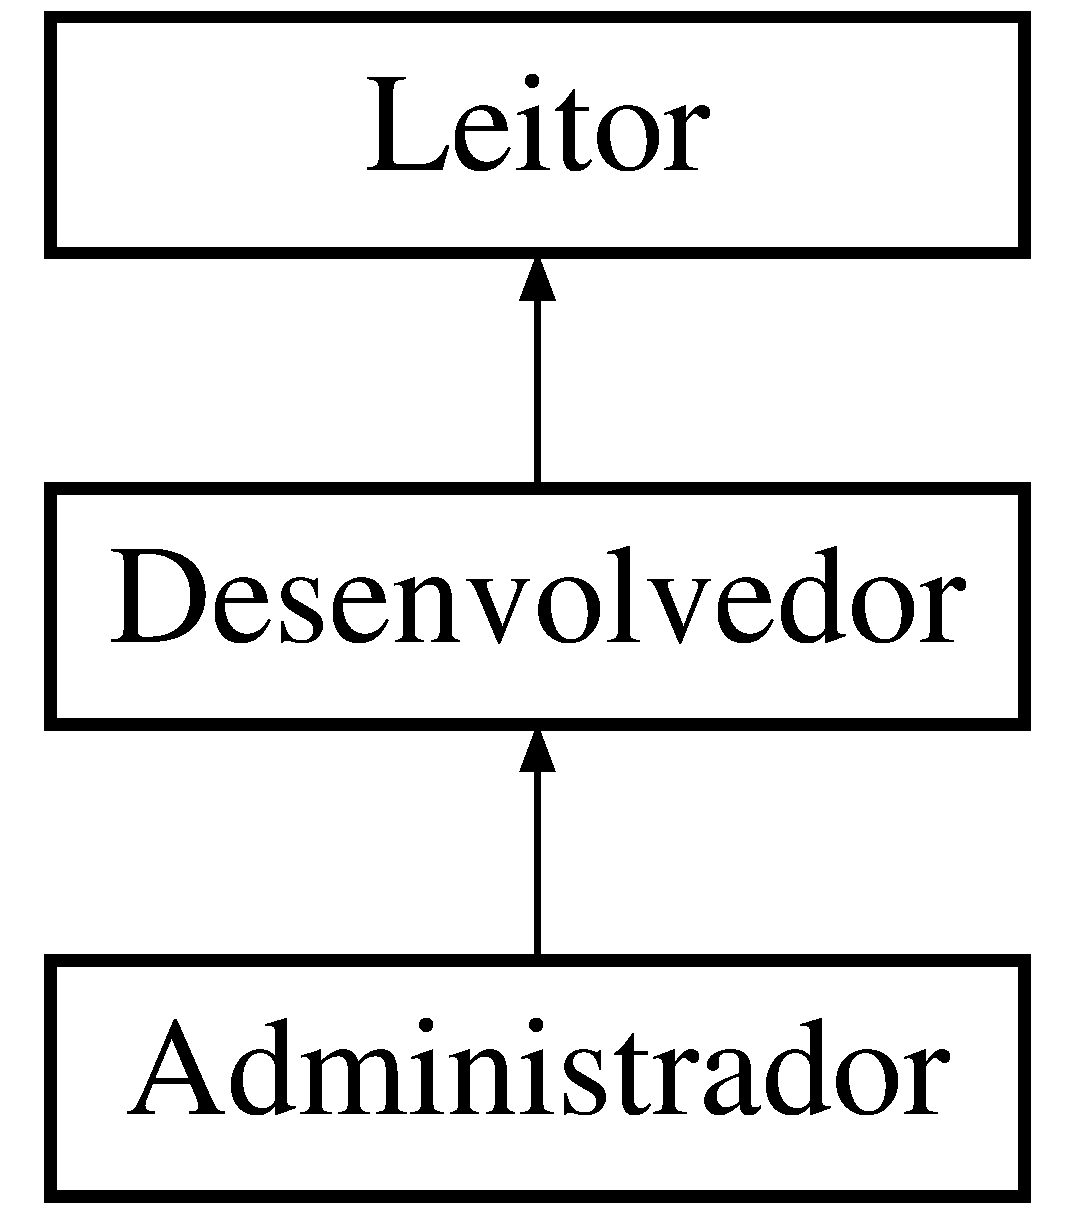
\includegraphics[height=3.000000cm]{class_administrador}
\end{center}
\end{figure}
\subsection*{Membros Públicos}
\begin{DoxyCompactItemize}
\item 
void \mbox{\hyperlink{class_administrador_ac841526561c3daf57f39ffd41e7211f2}{set\+Telefone}} (const \mbox{\hyperlink{class_telefone}{Telefone}} \&telefone)
\item 
\mbox{\hyperlink{class_telefone}{Telefone}} \mbox{\hyperlink{class_administrador_a2b7dddbf1e34a91a5f97c761332ce60b}{get\+Telefone}} ()
\item 
void \mbox{\hyperlink{class_administrador_afe7a5d85ee5c6a43a56b1a47daff358e}{set\+Endereco}} (const \mbox{\hyperlink{class_endereco}{Endereco}} \&endereco)
\item 
\mbox{\hyperlink{class_endereco}{Endereco}} \mbox{\hyperlink{class_administrador_a217b60a7f414efc581446eece222c6cf}{get\+Endereco}} ()
\end{DoxyCompactItemize}


\subsection{Descrição detalhada}
D\+E\+C\+L\+A\+R\+A\+C\+AO da classe A\+D\+M\+I\+N\+I\+S\+T\+R\+A\+D\+OR Esta classe herda todos os atributos da classe D\+E\+S\+E\+N\+V\+O\+L\+V\+E\+D\+OR que por consequencia herda os atributos da classe L\+E\+I\+T\+OR Possui dois novo atributos\+: \mbox{\hyperlink{class_telefone}{Telefone}} e Endereço que são dois objetos ~\newline
F\+U\+N\+C\+O\+ES E\+N\+T\+I\+D\+A\+DE A\+D\+M\+I\+N\+I\+S\+T\+R\+A\+D\+OR set\+Telefone get\+Telefone set\+Endereco get\+Endereco 

\subsection{Funções membros}
\mbox{\Hypertarget{class_administrador_a217b60a7f414efc581446eece222c6cf}\label{class_administrador_a217b60a7f414efc581446eece222c6cf}} 
\index{Administrador@{Administrador}!get\+Endereco@{get\+Endereco}}
\index{get\+Endereco@{get\+Endereco}!Administrador@{Administrador}}
\subsubsection{\texorpdfstring{get\+Endereco()}{getEndereco()}}
{\footnotesize\ttfamily \mbox{\hyperlink{class_endereco}{Endereco}} Administrador\+::get\+Endereco (\begin{DoxyParamCaption}{ }\end{DoxyParamCaption})\hspace{0.3cm}{\ttfamily [inline]}}


\begin{DoxyCode}
198   \{
199     \textcolor{keywordflow}{return} endereco;
200   \}
\end{DoxyCode}
\mbox{\Hypertarget{class_administrador_a2b7dddbf1e34a91a5f97c761332ce60b}\label{class_administrador_a2b7dddbf1e34a91a5f97c761332ce60b}} 
\index{Administrador@{Administrador}!get\+Telefone@{get\+Telefone}}
\index{get\+Telefone@{get\+Telefone}!Administrador@{Administrador}}
\subsubsection{\texorpdfstring{get\+Telefone()}{getTelefone()}}
{\footnotesize\ttfamily \mbox{\hyperlink{class_telefone}{Telefone}} Administrador\+::get\+Telefone (\begin{DoxyParamCaption}{ }\end{DoxyParamCaption})\hspace{0.3cm}{\ttfamily [inline]}}


\begin{DoxyCode}
188   \{
189     \textcolor{keywordflow}{return} telefone;
190   \}
\end{DoxyCode}
\mbox{\Hypertarget{class_administrador_afe7a5d85ee5c6a43a56b1a47daff358e}\label{class_administrador_afe7a5d85ee5c6a43a56b1a47daff358e}} 
\index{Administrador@{Administrador}!set\+Endereco@{set\+Endereco}}
\index{set\+Endereco@{set\+Endereco}!Administrador@{Administrador}}
\subsubsection{\texorpdfstring{set\+Endereco()}{setEndereco()}}
{\footnotesize\ttfamily void Administrador\+::set\+Endereco (\begin{DoxyParamCaption}\item[{const \mbox{\hyperlink{class_endereco}{Endereco}} \&}]{endereco }\end{DoxyParamCaption})\hspace{0.3cm}{\ttfamily [inline]}}


\begin{DoxyCode}
193   \{
194     this->endereco = endereco;
195   \}
\end{DoxyCode}
\mbox{\Hypertarget{class_administrador_ac841526561c3daf57f39ffd41e7211f2}\label{class_administrador_ac841526561c3daf57f39ffd41e7211f2}} 
\index{Administrador@{Administrador}!set\+Telefone@{set\+Telefone}}
\index{set\+Telefone@{set\+Telefone}!Administrador@{Administrador}}
\subsubsection{\texorpdfstring{set\+Telefone()}{setTelefone()}}
{\footnotesize\ttfamily void Administrador\+::set\+Telefone (\begin{DoxyParamCaption}\item[{const \mbox{\hyperlink{class_telefone}{Telefone}} \&}]{telefone }\end{DoxyParamCaption})\hspace{0.3cm}{\ttfamily [inline]}}


\begin{DoxyCode}
184   \{
185     this->telefone = telefone;
186   \}
\end{DoxyCode}


A documentação para essa classe foi gerada a partir do seguinte arquivo\+:\begin{DoxyCompactItemize}
\item 
/\+Users/amadeulinhares/\+Desktop/\+Trabalho3/\mbox{\hyperlink{entidades_8hpp}{entidades.\+hpp}}\end{DoxyCompactItemize}

\hypertarget{class_classe_termo}{}\section{Referência da Classe Classe\+Termo}
\label{class_classe_termo}\index{Classe\+Termo@{Classe\+Termo}}


{\ttfamily \#include $<$dominios.\+hpp$>$}

\subsection*{Membros Públicos}
\begin{DoxyCompactItemize}
\item 
void \mbox{\hyperlink{class_classe_termo_a9392585ac39c1ed25ad54f0902138457}{set\+Termo}} (string termo)
\item 
string \mbox{\hyperlink{class_classe_termo_acef132214ef8a667c9b9ca262fe7a9da}{get\+Termo}} ()
\item 
void \mbox{\hyperlink{class_classe_termo_a950f042edfb8e2e40caafba76a636c93}{verifica\+Termo}} (string termo)
\end{DoxyCompactItemize}


\subsection{Descrição detalhada}
D\+E\+C\+L\+A\+R\+A\+C\+AO C\+L\+A\+S\+SE -\/ C\+L\+A\+S\+SE DE T\+E\+R\+MO 

\subsection{Funções membros}
\mbox{\Hypertarget{class_classe_termo_acef132214ef8a667c9b9ca262fe7a9da}\label{class_classe_termo_acef132214ef8a667c9b9ca262fe7a9da}} 
\index{Classe\+Termo@{Classe\+Termo}!get\+Termo@{get\+Termo}}
\index{get\+Termo@{get\+Termo}!Classe\+Termo@{Classe\+Termo}}
\subsubsection{\texorpdfstring{get\+Termo()}{getTermo()}}
{\footnotesize\ttfamily string Classe\+Termo\+::get\+Termo (\begin{DoxyParamCaption}{ }\end{DoxyParamCaption})}


\begin{DoxyCode}
495 \{
496   \textcolor{keywordflow}{return} this->termo;
497 \}
\end{DoxyCode}
\mbox{\Hypertarget{class_classe_termo_a9392585ac39c1ed25ad54f0902138457}\label{class_classe_termo_a9392585ac39c1ed25ad54f0902138457}} 
\index{Classe\+Termo@{Classe\+Termo}!set\+Termo@{set\+Termo}}
\index{set\+Termo@{set\+Termo}!Classe\+Termo@{Classe\+Termo}}
\subsubsection{\texorpdfstring{set\+Termo()}{setTermo()}}
{\footnotesize\ttfamily void Classe\+Termo\+::set\+Termo (\begin{DoxyParamCaption}\item[{string}]{termo }\end{DoxyParamCaption})}


\begin{DoxyCode}
489 \{
490   \mbox{\hyperlink{class_classe_termo_a950f042edfb8e2e40caafba76a636c93}{verificaTermo}}(termo);
491   this->termo = termo;
492 \}
\end{DoxyCode}
\mbox{\Hypertarget{class_classe_termo_a950f042edfb8e2e40caafba76a636c93}\label{class_classe_termo_a950f042edfb8e2e40caafba76a636c93}} 
\index{Classe\+Termo@{Classe\+Termo}!verifica\+Termo@{verifica\+Termo}}
\index{verifica\+Termo@{verifica\+Termo}!Classe\+Termo@{Classe\+Termo}}
\subsubsection{\texorpdfstring{verifica\+Termo()}{verificaTermo()}}
{\footnotesize\ttfamily void Classe\+Termo\+::verifica\+Termo (\begin{DoxyParamCaption}\item[{string}]{termo }\end{DoxyParamCaption})}


\begin{DoxyCode}
500 \{
501   \textcolor{keywordflow}{if}((termo != \textcolor{stringliteral}{"PT"}) && (termo != \textcolor{stringliteral}{"NP"}))
502   \{
503     \textcolor{keywordflow}{throw}\textcolor{stringliteral}{"Erro: Termo Invalido\(\backslash\)n"};
504   \}
505 \}
\end{DoxyCode}


A documentação para essa classe foi gerada a partir dos seguintes arquivos\+:\begin{DoxyCompactItemize}
\item 
/\+Users/amadeulinhares/\+Desktop/\+Trabalho3/\mbox{\hyperlink{dominios_8hpp}{dominios.\+hpp}}\item 
/\+Users/amadeulinhares/\+Desktop/\+Trabalho3/\mbox{\hyperlink{dominios_8cpp}{dominios.\+cpp}}\end{DoxyCompactItemize}

\hypertarget{class_controladora_apresentacao}{}\section{Referência da Classe Controladora\+Apresentacao}
\label{class_controladora_apresentacao}\index{Controladora\+Apresentacao@{Controladora\+Apresentacao}}


{\ttfamily \#include $<$controladoras.\+hpp$>$}

Diagrama de hierarquia para Controladora\+Apresentacao\+:\begin{figure}[H]
\begin{center}
\leavevmode
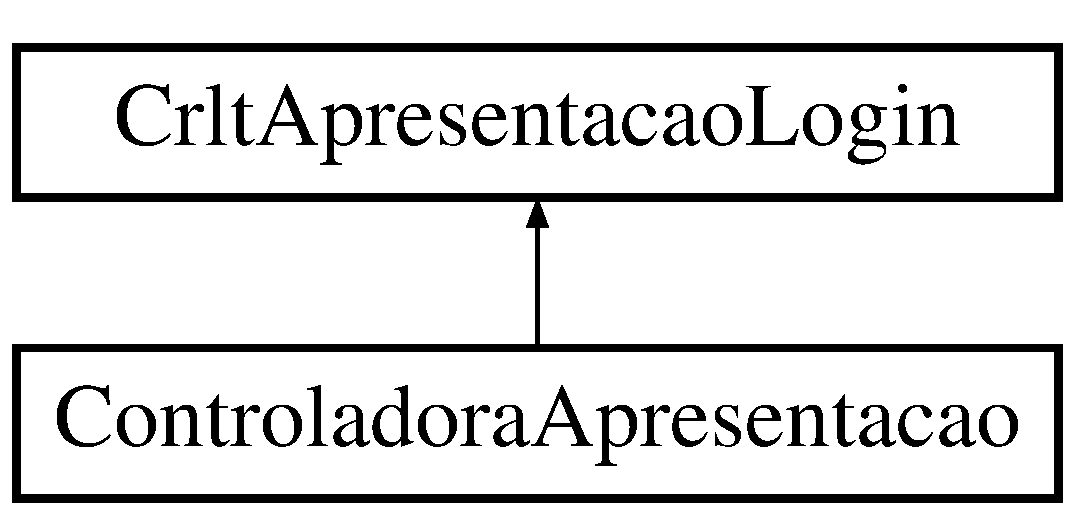
\includegraphics[height=2.000000cm]{class_controladora_apresentacao}
\end{center}
\end{figure}
\subsection*{Membros Públicos}
\begin{DoxyCompactItemize}
\item 
int \mbox{\hyperlink{class_controladora_apresentacao_a303849d9fd6785bcbdd5c96fb2413ef3}{menu}} ()
\end{DoxyCompactItemize}


\subsection{Descrição detalhada}
Parte do trabalho que possui a declaracao de duas classes, a primeira sendo a \mbox{\hyperlink{class_controladora_apresentacao}{Controladora\+Apresentacao}} que herda os metodos da classe Interface\+Apresentacao e a segunda sendo Controladora\+Usuario que herda os metodos da classe Interface\+Apresentacao\+Usuario 

\subsection{Funções membros}
\mbox{\Hypertarget{class_controladora_apresentacao_a303849d9fd6785bcbdd5c96fb2413ef3}\label{class_controladora_apresentacao_a303849d9fd6785bcbdd5c96fb2413ef3}} 
\index{Controladora\+Apresentacao@{Controladora\+Apresentacao}!menu@{menu}}
\index{menu@{menu}!Controladora\+Apresentacao@{Controladora\+Apresentacao}}
\subsubsection{\texorpdfstring{menu()}{menu()}}
{\footnotesize\ttfamily int Controladora\+Apresentacao\+::menu (\begin{DoxyParamCaption}{ }\end{DoxyParamCaption})\hspace{0.3cm}{\ttfamily [virtual]}}

Primeiramente temos o metodo validar da classe \mbox{\hyperlink{class_controladora_apresentacao_usuario}{Controladora\+Apresentacao\+Usuario}}. Esse metodo pede um nome, e-\/mail e senha do usuario do programa, jogando esses informacoes dentro de objetos criados ao inicio do metodo Colocado dentro de um while, o usuario do pode logar se suas informacoes bateram com as Triggers de informacoes, existindo uma para cada tipo de usuario possivel do sistema (\mbox{\hyperlink{class_leitor}{Leitor}}, desenvolvedor e administrador) Se as informacoes foram colocadas corretamente, o metodo ira retornar o e-\/mail digitado pelo usuario, onde de acordo com esse e-\/mail retornado para o main, o programa ira identificar qual o tipo de Usuario e criar os devidos objetos para cada um deles.

O proximo metodo se chama opcao\+Leitor(), onde esse metodo ira mostrar as opcoes para o usurio que faça o login como \mbox{\hyperlink{class_leitor}{Leitor}} no sistema. O metodo consiste em um while que mostra as opcoes do sistema e so saira do while quando o usuario escolher uma opcao valida. Esse numero de opcao sera armazenado em uma variavel e retornado para a funcao main, onde sera aproveitado em outro metodo que veremos na aba das Stubs.\+cpp

O proximo metodo se chama opcao\+Desenvolvedor(), onde esse metodo ira mostrar as opcoes para o usurio que faça o login como \mbox{\hyperlink{class_desenvolvedor}{Desenvolvedor}} no sistema. O metodo consiste em um while que mostra as opcoes do sistema e so saira do while quando o usuario escolher uma opcao valida. Esse numero de opcao sera armazenado em uma variavel e retornado para a funcao main, onde sera aproveitado em outro metodo que veremos na aba das Stubs.\+cpp

O proximo metodo se chama opcao\+Administrador(), onde esse metodo ira mostrar as opcoes para o usurio que faça o login como \mbox{\hyperlink{class_administrador}{Administrador}} no sistema. O metodo consiste em um while que mostra as opcoes do sistema e so saira do while quando o usuario escolher uma opcao valida. Esse numero de opcao sera armazenado em uma variavel e retornado para a funcao main, onde sera aproveitado em outro metodo que veremos na aba das Stubs.\+cpp 

Implementa \mbox{\hyperlink{class_crlt_apresentacao_login_a76226b00329c638d6de95458ad87756e}{Crlt\+Apresentacao\+Login}}.


\begin{DoxyCode}
22 \{
23   \textcolor{keywordtype}{int} opcao;
24   \textcolor{keywordflow}{while}(\textcolor{keyword}{true})
25   \{
26     cout <<    \textcolor{stringliteral}{"\(\backslash\)n\(\backslash\)t\(\backslash\)t Vocabulario Controlado "}   <<\textcolor{stringliteral}{"\(\backslash\)n"}<<endl;
27     cout << \textcolor{stringliteral}{"\(\backslash\)t1- Logar como Leitor\(\backslash\)n"};
28     cout << \textcolor{stringliteral}{"\(\backslash\)t2- Logar como Desenvolvedor\(\backslash\)n"};
29     cout << \textcolor{stringliteral}{"\(\backslash\)t3- Logar como Administrador\(\backslash\)n"};
30     cout << \textcolor{stringliteral}{"\(\backslash\)t4- Criar conta\(\backslash\)n\(\backslash\)n"};
31 
32     cout << \textcolor{stringliteral}{"\(\backslash\)t*Digite a opcao escolhida: "};
33     cin >> opcao;
34 
35     \textcolor{keywordflow}{if}((opcao != 1) && (opcao != 2) && (opcao != 3) && (opcao != 4))
36     \{
37       cout << \textcolor{stringliteral}{"\(\backslash\)n\(\backslash\)t\(\backslash\)tOpcao invalida, tente novamente\(\backslash\)n\(\backslash\)n"};
38     \}
39     \textcolor{keywordflow}{else}
40     \{
41       \textcolor{keywordflow}{break};
42     \}
43   \}
44 
45   \textcolor{keywordflow}{return} opcao;
46 \}
\end{DoxyCode}


A documentação para essa classe foi gerada a partir dos seguintes arquivos\+:\begin{DoxyCompactItemize}
\item 
/\+Users/amadeulinhares/\+Desktop/\+Trabalho3/\mbox{\hyperlink{controladoras_8hpp}{controladoras.\+hpp}}\item 
/\+Users/amadeulinhares/\+Desktop/\+Trabalho3/\mbox{\hyperlink{controladoras_8cpp}{controladoras.\+cpp}}\end{DoxyCompactItemize}

\hypertarget{class_controladora_apresentacao_usuario}{}\section{Referência da Classe Controladora\+Apresentacao\+Usuario}
\label{class_controladora_apresentacao_usuario}\index{Controladora\+Apresentacao\+Usuario@{Controladora\+Apresentacao\+Usuario}}


{\ttfamily \#include $<$controladoras.\+hpp$>$}

Diagrama de hierarquia para Controladora\+Apresentacao\+Usuario\+:\begin{figure}[H]
\begin{center}
\leavevmode
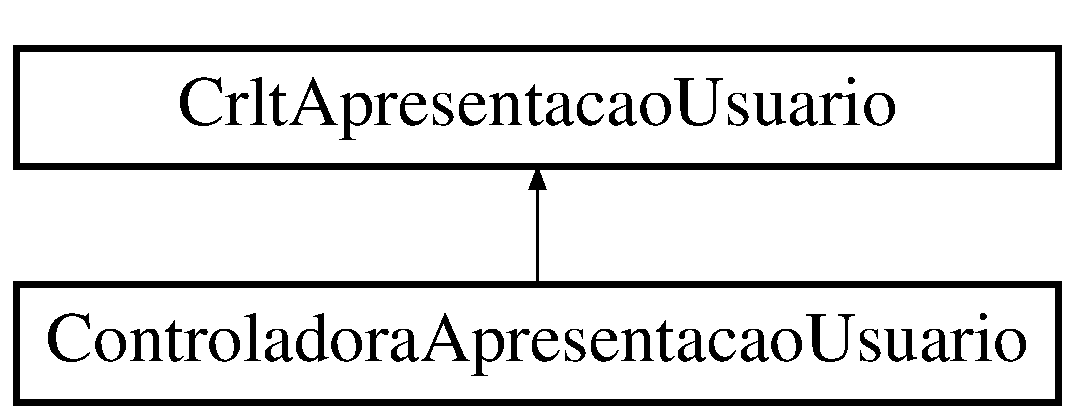
\includegraphics[height=2.000000cm]{class_controladora_apresentacao_usuario}
\end{center}
\end{figure}
\subsection*{Membros Públicos}
\begin{DoxyCompactItemize}
\item 
int \mbox{\hyperlink{class_controladora_apresentacao_usuario_a22b31c99a738845f00ec2703c1c6dded}{opcao\+Leitor}} ()
\item 
int \mbox{\hyperlink{class_controladora_apresentacao_usuario_a1d9f2e8522d9e0eefaf08caca98008c2}{opcao\+Desenvolvedor}} ()
\item 
int \mbox{\hyperlink{class_controladora_apresentacao_usuario_ae4d0223e4aabe11b58039c84c80503c9}{opcao\+Administrador}} ()
\end{DoxyCompactItemize}


\subsection{Funções membros}
\mbox{\Hypertarget{class_controladora_apresentacao_usuario_ae4d0223e4aabe11b58039c84c80503c9}\label{class_controladora_apresentacao_usuario_ae4d0223e4aabe11b58039c84c80503c9}} 
\index{Controladora\+Apresentacao\+Usuario@{Controladora\+Apresentacao\+Usuario}!opcao\+Administrador@{opcao\+Administrador}}
\index{opcao\+Administrador@{opcao\+Administrador}!Controladora\+Apresentacao\+Usuario@{Controladora\+Apresentacao\+Usuario}}
\subsubsection{\texorpdfstring{opcao\+Administrador()}{opcaoAdministrador()}}
{\footnotesize\ttfamily int Controladora\+Apresentacao\+Usuario\+::opcao\+Administrador (\begin{DoxyParamCaption}{ }\end{DoxyParamCaption})\hspace{0.3cm}{\ttfamily [virtual]}}



Implementa \mbox{\hyperlink{class_crlt_apresentacao_usuario_aa4e0600a397ea82224441793424d7daa}{Crlt\+Apresentacao\+Usuario}}.


\begin{DoxyCode}
124 \{
125   \textcolor{keywordtype}{int} entrada;
126   \textcolor{keywordtype}{int} aux = 0;
127   \textcolor{keywordflow}{while}(aux == 0)
128   \{
129       cout << \textcolor{stringliteral}{"Opções para Usuario Desenvolvedor\(\backslash\)n"} << endl;
130       cout << \textcolor{stringliteral}{"1- Apresentar dados do Usúario\(\backslash\)n"};
131       cout << \textcolor{stringliteral}{"2- Editar dados do Usuario\(\backslash\)n"};
132       cout << \textcolor{stringliteral}{"3- Excluir Conta\(\backslash\)n"};
133       cout << \textcolor{stringliteral}{"4- Listar nomes dos vocabularios controlados\(\backslash\)n"};
134       cout << \textcolor{stringliteral}{"5- Dados do vocabulario controlado\(\backslash\)n"};
135       cout << \textcolor{stringliteral}{"6- Consultar Termo\(\backslash\)n"};
136       cout << \textcolor{stringliteral}{"7- Consultar definição de termos\(\backslash\)n"};
137       cout << \textcolor{stringliteral}{"8- Cadastro desenvolvedor de vocabulario controlado\(\backslash\)n"};
138       cout << \textcolor{stringliteral}{"9- Criar Termo\(\backslash\)n"};
139       cout << \textcolor{stringliteral}{"10- Editar Termo\(\backslash\)n"};
140       cout << \textcolor{stringliteral}{"11- Excluir Termo\(\backslash\)n"};
141       cout << \textcolor{stringliteral}{"12- Criar definicao para termo\(\backslash\)n"};
142       cout << \textcolor{stringliteral}{"13- Excluir definicao de termo\(\backslash\)n"};
143       cout << \textcolor{stringliteral}{"14- Editar definicao de termo \(\backslash\)n"};
144       cout << \textcolor{stringliteral}{"15- Criar Vocabulario controlado\(\backslash\)n"};
145       cout << \textcolor{stringliteral}{"16- Editar definicao de vocabulario controlado\(\backslash\)n"};
146       cout << \textcolor{stringliteral}{"17- Alterar idioma de vocabulario controlado\(\backslash\)n"};
147       cout << \textcolor{stringliteral}{"18- Excluir Vocabulario Controlado\(\backslash\)n"};
148       cout << \textcolor{stringliteral}{"Digite a opçāo desejada: "};
149       cin >> entrada;
150       cout << \textcolor{stringliteral}{"\(\backslash\)n"};
151       \textcolor{keywordflow}{if}(entrada < 1 || entrada > 18)
152       \{
153         cout << \textcolor{stringliteral}{"Erro, Opçao invalida.....\(\backslash\)n"} << endl;
154         cout << \textcolor{stringliteral}{"Retornando para o Menu de escolhas \(\backslash\)n"} << endl;
155       \}
156       \textcolor{keywordflow}{else}
157       \{
158         aux = 1;
159       \}
160   \}
161   \textcolor{keywordflow}{return} entrada;
162 \}
\end{DoxyCode}
\mbox{\Hypertarget{class_controladora_apresentacao_usuario_a1d9f2e8522d9e0eefaf08caca98008c2}\label{class_controladora_apresentacao_usuario_a1d9f2e8522d9e0eefaf08caca98008c2}} 
\index{Controladora\+Apresentacao\+Usuario@{Controladora\+Apresentacao\+Usuario}!opcao\+Desenvolvedor@{opcao\+Desenvolvedor}}
\index{opcao\+Desenvolvedor@{opcao\+Desenvolvedor}!Controladora\+Apresentacao\+Usuario@{Controladora\+Apresentacao\+Usuario}}
\subsubsection{\texorpdfstring{opcao\+Desenvolvedor()}{opcaoDesenvolvedor()}}
{\footnotesize\ttfamily int Controladora\+Apresentacao\+Usuario\+::opcao\+Desenvolvedor (\begin{DoxyParamCaption}{ }\end{DoxyParamCaption})\hspace{0.3cm}{\ttfamily [virtual]}}



Implementa \mbox{\hyperlink{class_crlt_apresentacao_usuario_ad9091cb4093bdc687c0deffb5b00512c}{Crlt\+Apresentacao\+Usuario}}.


\begin{DoxyCode}
82 \{
83   \textcolor{keywordtype}{int} entrada;
84   \textcolor{keywordtype}{int} aux = 0;
85   \textcolor{keywordflow}{while}(aux == 0)
86   \{
87       cout << \textcolor{stringliteral}{"Opções para Usuario Desenvolvedor\(\backslash\)n"} << endl;
88       cout << \textcolor{stringliteral}{"1- Apresentar dados do Usúario\(\backslash\)n"};
89       cout << \textcolor{stringliteral}{"2- Editar dados do Usuario\(\backslash\)n"};
90       cout << \textcolor{stringliteral}{"3- Excluir Conta\(\backslash\)n"};
91       cout << \textcolor{stringliteral}{"4- Listar nomes dos vocabularios controlados\(\backslash\)n"};
92       cout << \textcolor{stringliteral}{"5- Dados do vocabulario controlado\(\backslash\)n"};
93       cout << \textcolor{stringliteral}{"6- Consultar Termo\(\backslash\)n"};
94       cout << \textcolor{stringliteral}{"7- Consultar definição de termos\(\backslash\)n"};
95       cout << \textcolor{stringliteral}{"8- Cadastro desenvolvedor de vocabulario controlado\(\backslash\)n"};
96       cout << \textcolor{stringliteral}{"9- Criar Termo\(\backslash\)n"};
97       cout << \textcolor{stringliteral}{"10- Editar Termo\(\backslash\)n"};
98       cout << \textcolor{stringliteral}{"11- Excluir Termo\(\backslash\)n"};
99       cout << \textcolor{stringliteral}{"12- Criar definicao para termo\(\backslash\)n"};
100       cout << \textcolor{stringliteral}{"13- Excluir definicao de termo\(\backslash\)n"};
101       cout << \textcolor{stringliteral}{"14- Editar definicao de termo \(\backslash\)n\(\backslash\)n"};
102       cout << \textcolor{stringliteral}{"Digite a opçāo desejada: "};
103       cin >> entrada;
104       cout << \textcolor{stringliteral}{"\(\backslash\)n"};
105       \textcolor{keywordflow}{if}(entrada < 1 || entrada > 14)
106       \{
107         cout << \textcolor{stringliteral}{"Erro, Opçao invalida.....\(\backslash\)n"} << endl;
108         cout << \textcolor{stringliteral}{"Retornando para o Menu de escolhas \(\backslash\)n"} << endl;
109       \}
110       \textcolor{keywordflow}{else}
111       \{
112         aux = 1;
113       \}
114   \}
115   \textcolor{keywordflow}{return} entrada;
116 \}
\end{DoxyCode}
\mbox{\Hypertarget{class_controladora_apresentacao_usuario_a22b31c99a738845f00ec2703c1c6dded}\label{class_controladora_apresentacao_usuario_a22b31c99a738845f00ec2703c1c6dded}} 
\index{Controladora\+Apresentacao\+Usuario@{Controladora\+Apresentacao\+Usuario}!opcao\+Leitor@{opcao\+Leitor}}
\index{opcao\+Leitor@{opcao\+Leitor}!Controladora\+Apresentacao\+Usuario@{Controladora\+Apresentacao\+Usuario}}
\subsubsection{\texorpdfstring{opcao\+Leitor()}{opcaoLeitor()}}
{\footnotesize\ttfamily int Controladora\+Apresentacao\+Usuario\+::opcao\+Leitor (\begin{DoxyParamCaption}{ }\end{DoxyParamCaption})\hspace{0.3cm}{\ttfamily [virtual]}}



Implementa \mbox{\hyperlink{class_crlt_apresentacao_usuario_a627dcf5329233dee6ef2888dacf8a5a1}{Crlt\+Apresentacao\+Usuario}}.


\begin{DoxyCode}
52 \{
53   \textcolor{keywordtype}{int} entrada;
54   \textcolor{keywordtype}{int} aux = 0;
55   \textcolor{keywordflow}{while}(aux == 0)
56   \{
57       cout << \textcolor{stringliteral}{"Opções para Usuario Leitor\(\backslash\)n"} << endl;
58       cout << \textcolor{stringliteral}{"1- Apresentar dados do Usúario\(\backslash\)n"};
59       cout << \textcolor{stringliteral}{"2- Editar dados do Usuario\(\backslash\)n"};
60       cout << \textcolor{stringliteral}{"3- Excluir Conta\(\backslash\)n"};
61       cout << \textcolor{stringliteral}{"4- Listar nomes dos vocabularios controlados\(\backslash\)n"};
62       cout << \textcolor{stringliteral}{"5- Dados do vocabulario controlado\(\backslash\)n"};
63       cout << \textcolor{stringliteral}{"6- Consultar Termo\(\backslash\)n"};
64       cout << \textcolor{stringliteral}{"7- Consultar definição de termos\(\backslash\)n\(\backslash\)n"};
65       cout << \textcolor{stringliteral}{"Digite a opçāo desejada: "};
66       cin >> entrada;
67       cout << \textcolor{stringliteral}{"\(\backslash\)n"};
68       \textcolor{keywordflow}{if}(entrada < 1 || entrada > 7)
69       \{
70         cout << \textcolor{stringliteral}{"Erro, Opçao invalida.....\(\backslash\)n"} << endl;
71         cout << \textcolor{stringliteral}{"Retornando para o Menu de escolhas \(\backslash\)n"} << endl;
72       \}
73       \textcolor{keywordflow}{else}
74       \{
75         aux = 1;
76       \}
77   \}
78   \textcolor{keywordflow}{return} entrada;
79 \}
\end{DoxyCode}


A documentação para essa classe foi gerada a partir dos seguintes arquivos\+:\begin{DoxyCompactItemize}
\item 
/\+Users/amadeulinhares/\+Desktop/\+Trabalho3/\mbox{\hyperlink{controladoras_8hpp}{controladoras.\+hpp}}\item 
/\+Users/amadeulinhares/\+Desktop/\+Trabalho3/\mbox{\hyperlink{controladoras_8cpp}{controladoras.\+cpp}}\end{DoxyCompactItemize}

\hypertarget{class_crlt_apresentacao_login}{}\section{Referência da Classe Crlt\+Apresentacao\+Login}
\label{class_crlt_apresentacao_login}\index{Crlt\+Apresentacao\+Login@{Crlt\+Apresentacao\+Login}}


{\ttfamily \#include $<$interface.\+hpp$>$}

Diagrama de hierarquia para Crlt\+Apresentacao\+Login\+:\begin{figure}[H]
\begin{center}
\leavevmode
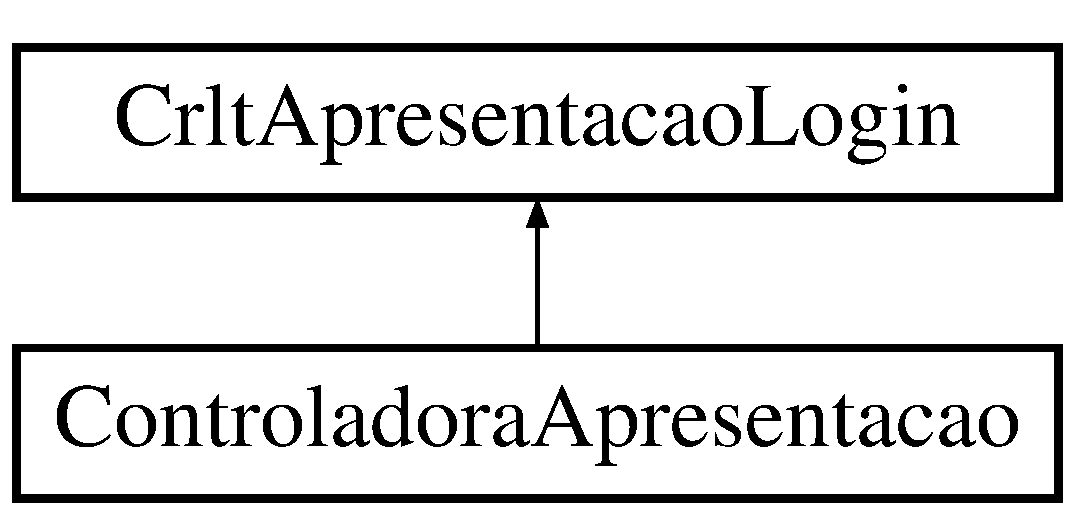
\includegraphics[height=2.000000cm]{class_crlt_apresentacao_login}
\end{center}
\end{figure}
\subsection*{Membros Públicos}
\begin{DoxyCompactItemize}
\item 
virtual int \mbox{\hyperlink{class_crlt_apresentacao_login_a76226b00329c638d6de95458ad87756e}{menu}} ()=0
\item 
virtual \mbox{\hyperlink{class_crlt_apresentacao_login_a8fba6ea4b607b28d377af308d617aa05}{$\sim$\+Crlt\+Apresentacao\+Login}} ()
\end{DoxyCompactItemize}


\subsection{Construtores e Destrutores}
\mbox{\Hypertarget{class_crlt_apresentacao_login_a8fba6ea4b607b28d377af308d617aa05}\label{class_crlt_apresentacao_login_a8fba6ea4b607b28d377af308d617aa05}} 
\index{Crlt\+Apresentacao\+Login@{Crlt\+Apresentacao\+Login}!````~Crlt\+Apresentacao\+Login@{$\sim$\+Crlt\+Apresentacao\+Login}}
\index{````~Crlt\+Apresentacao\+Login@{$\sim$\+Crlt\+Apresentacao\+Login}!Crlt\+Apresentacao\+Login@{Crlt\+Apresentacao\+Login}}
\subsubsection{\texorpdfstring{$\sim$\+Crlt\+Apresentacao\+Login()}{~CrltApresentacaoLogin()}}
{\footnotesize\ttfamily virtual Crlt\+Apresentacao\+Login\+::$\sim$\+Crlt\+Apresentacao\+Login (\begin{DoxyParamCaption}{ }\end{DoxyParamCaption})\hspace{0.3cm}{\ttfamily [inline]}, {\ttfamily [virtual]}}


\begin{DoxyCode}
11 \{\}
\end{DoxyCode}


\subsection{Funções membros}
\mbox{\Hypertarget{class_crlt_apresentacao_login_a76226b00329c638d6de95458ad87756e}\label{class_crlt_apresentacao_login_a76226b00329c638d6de95458ad87756e}} 
\index{Crlt\+Apresentacao\+Login@{Crlt\+Apresentacao\+Login}!menu@{menu}}
\index{menu@{menu}!Crlt\+Apresentacao\+Login@{Crlt\+Apresentacao\+Login}}
\subsubsection{\texorpdfstring{menu()}{menu()}}
{\footnotesize\ttfamily virtual int Crlt\+Apresentacao\+Login\+::menu (\begin{DoxyParamCaption}{ }\end{DoxyParamCaption})\hspace{0.3cm}{\ttfamily [pure virtual]}}



Implementado por \mbox{\hyperlink{class_controladora_apresentacao_a303849d9fd6785bcbdd5c96fb2413ef3}{Controladora\+Apresentacao}}.



A documentação para essa classe foi gerada a partir do seguinte arquivo\+:\begin{DoxyCompactItemize}
\item 
/\+Users/amadeulinhares/\+Desktop/\+Trabalho3/\mbox{\hyperlink{interface_8hpp}{interface.\+hpp}}\end{DoxyCompactItemize}

\hypertarget{class_crlt_apresentacao_usuario}{}\section{Referência da Classe Crlt\+Apresentacao\+Usuario}
\label{class_crlt_apresentacao_usuario}\index{Crlt\+Apresentacao\+Usuario@{Crlt\+Apresentacao\+Usuario}}


{\ttfamily \#include $<$interface.\+hpp$>$}

Diagrama de hierarquia para Crlt\+Apresentacao\+Usuario\+:\begin{figure}[H]
\begin{center}
\leavevmode
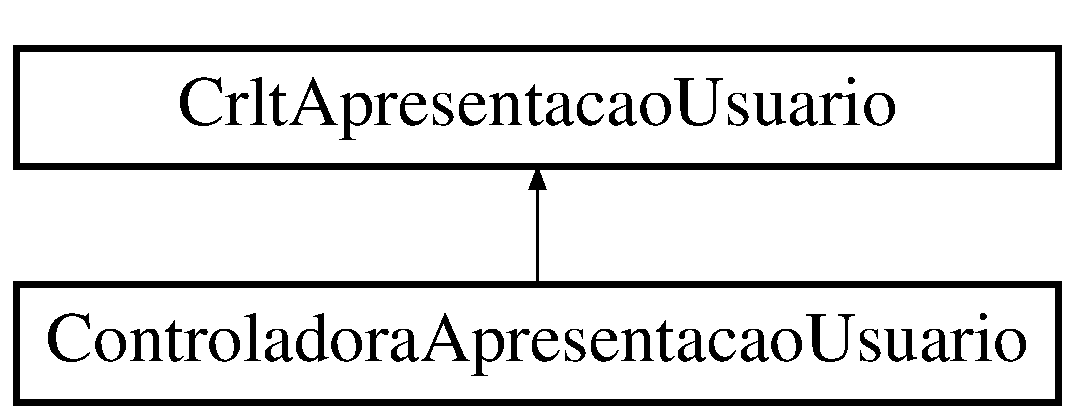
\includegraphics[height=2.000000cm]{class_crlt_apresentacao_usuario}
\end{center}
\end{figure}
\subsection*{Membros Públicos}
\begin{DoxyCompactItemize}
\item 
virtual int \mbox{\hyperlink{class_crlt_apresentacao_usuario_a627dcf5329233dee6ef2888dacf8a5a1}{opcao\+Leitor}} ()=0
\item 
virtual int \mbox{\hyperlink{class_crlt_apresentacao_usuario_ad9091cb4093bdc687c0deffb5b00512c}{opcao\+Desenvolvedor}} ()=0
\item 
virtual int \mbox{\hyperlink{class_crlt_apresentacao_usuario_aa4e0600a397ea82224441793424d7daa}{opcao\+Administrador}} ()=0
\item 
\mbox{\hyperlink{class_crlt_apresentacao_usuario_a27e014ae8177823f6e9575b7d0b64717}{$\sim$\+Crlt\+Apresentacao\+Usuario}} ()
\end{DoxyCompactItemize}


\subsection{Construtores e Destrutores}
\mbox{\Hypertarget{class_crlt_apresentacao_usuario_a27e014ae8177823f6e9575b7d0b64717}\label{class_crlt_apresentacao_usuario_a27e014ae8177823f6e9575b7d0b64717}} 
\index{Crlt\+Apresentacao\+Usuario@{Crlt\+Apresentacao\+Usuario}!````~Crlt\+Apresentacao\+Usuario@{$\sim$\+Crlt\+Apresentacao\+Usuario}}
\index{````~Crlt\+Apresentacao\+Usuario@{$\sim$\+Crlt\+Apresentacao\+Usuario}!Crlt\+Apresentacao\+Usuario@{Crlt\+Apresentacao\+Usuario}}
\subsubsection{\texorpdfstring{$\sim$\+Crlt\+Apresentacao\+Usuario()}{~CrltApresentacaoUsuario()}}
{\footnotesize\ttfamily Crlt\+Apresentacao\+Usuario\+::$\sim$\+Crlt\+Apresentacao\+Usuario (\begin{DoxyParamCaption}{ }\end{DoxyParamCaption})\hspace{0.3cm}{\ttfamily [inline]}}


\begin{DoxyCode}
40 \{\}
\end{DoxyCode}


\subsection{Funções membros}
\mbox{\Hypertarget{class_crlt_apresentacao_usuario_aa4e0600a397ea82224441793424d7daa}\label{class_crlt_apresentacao_usuario_aa4e0600a397ea82224441793424d7daa}} 
\index{Crlt\+Apresentacao\+Usuario@{Crlt\+Apresentacao\+Usuario}!opcao\+Administrador@{opcao\+Administrador}}
\index{opcao\+Administrador@{opcao\+Administrador}!Crlt\+Apresentacao\+Usuario@{Crlt\+Apresentacao\+Usuario}}
\subsubsection{\texorpdfstring{opcao\+Administrador()}{opcaoAdministrador()}}
{\footnotesize\ttfamily virtual int Crlt\+Apresentacao\+Usuario\+::opcao\+Administrador (\begin{DoxyParamCaption}{ }\end{DoxyParamCaption})\hspace{0.3cm}{\ttfamily [pure virtual]}}



Implementado por \mbox{\hyperlink{class_controladora_apresentacao_usuario_ae4d0223e4aabe11b58039c84c80503c9}{Controladora\+Apresentacao\+Usuario}}.

\mbox{\Hypertarget{class_crlt_apresentacao_usuario_ad9091cb4093bdc687c0deffb5b00512c}\label{class_crlt_apresentacao_usuario_ad9091cb4093bdc687c0deffb5b00512c}} 
\index{Crlt\+Apresentacao\+Usuario@{Crlt\+Apresentacao\+Usuario}!opcao\+Desenvolvedor@{opcao\+Desenvolvedor}}
\index{opcao\+Desenvolvedor@{opcao\+Desenvolvedor}!Crlt\+Apresentacao\+Usuario@{Crlt\+Apresentacao\+Usuario}}
\subsubsection{\texorpdfstring{opcao\+Desenvolvedor()}{opcaoDesenvolvedor()}}
{\footnotesize\ttfamily virtual int Crlt\+Apresentacao\+Usuario\+::opcao\+Desenvolvedor (\begin{DoxyParamCaption}{ }\end{DoxyParamCaption})\hspace{0.3cm}{\ttfamily [pure virtual]}}



Implementado por \mbox{\hyperlink{class_controladora_apresentacao_usuario_a1d9f2e8522d9e0eefaf08caca98008c2}{Controladora\+Apresentacao\+Usuario}}.

\mbox{\Hypertarget{class_crlt_apresentacao_usuario_a627dcf5329233dee6ef2888dacf8a5a1}\label{class_crlt_apresentacao_usuario_a627dcf5329233dee6ef2888dacf8a5a1}} 
\index{Crlt\+Apresentacao\+Usuario@{Crlt\+Apresentacao\+Usuario}!opcao\+Leitor@{opcao\+Leitor}}
\index{opcao\+Leitor@{opcao\+Leitor}!Crlt\+Apresentacao\+Usuario@{Crlt\+Apresentacao\+Usuario}}
\subsubsection{\texorpdfstring{opcao\+Leitor()}{opcaoLeitor()}}
{\footnotesize\ttfamily virtual int Crlt\+Apresentacao\+Usuario\+::opcao\+Leitor (\begin{DoxyParamCaption}{ }\end{DoxyParamCaption})\hspace{0.3cm}{\ttfamily [pure virtual]}}



Implementado por \mbox{\hyperlink{class_controladora_apresentacao_usuario_a22b31c99a738845f00ec2703c1c6dded}{Controladora\+Apresentacao\+Usuario}}.



A documentação para essa classe foi gerada a partir do seguinte arquivo\+:\begin{DoxyCompactItemize}
\item 
/\+Users/amadeulinhares/\+Desktop/\+Trabalho3/\mbox{\hyperlink{interface_8hpp}{interface.\+hpp}}\end{DoxyCompactItemize}

\hypertarget{class_crlt_servico_login}{}\section{Referência da Classe Crlt\+Servico\+Login}
\label{class_crlt_servico_login}\index{Crlt\+Servico\+Login@{Crlt\+Servico\+Login}}


{\ttfamily \#include $<$interface.\+hpp$>$}

Diagrama de hierarquia para Crlt\+Servico\+Login\+:\begin{figure}[H]
\begin{center}
\leavevmode
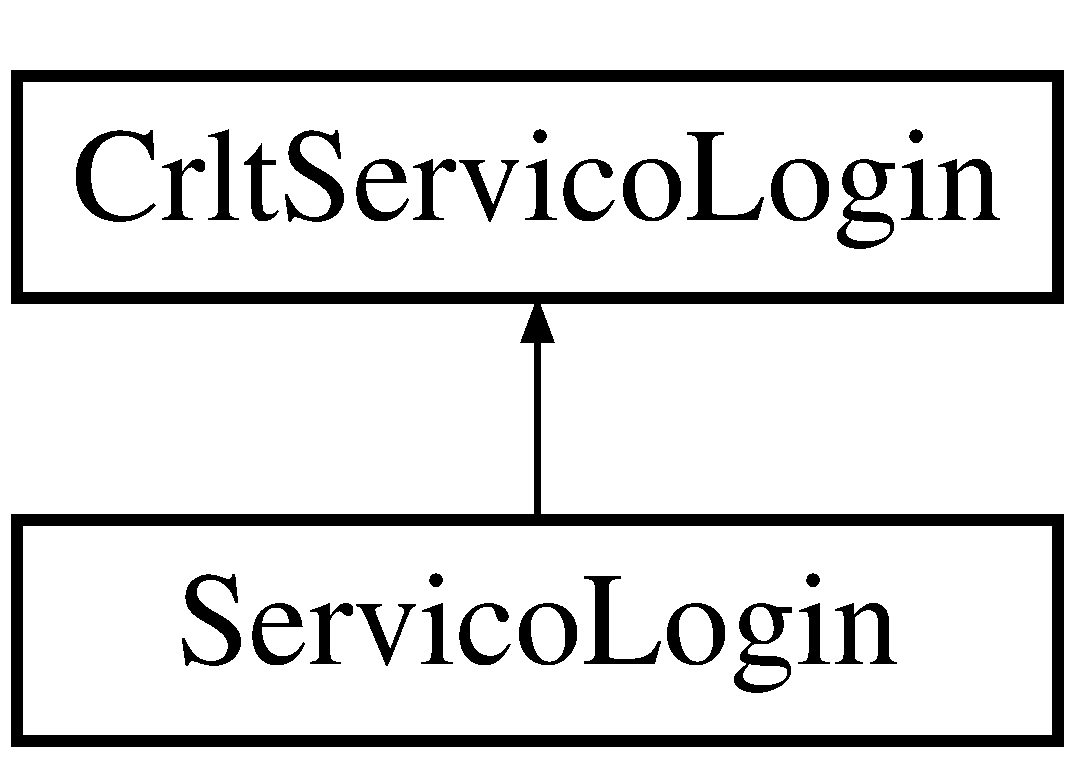
\includegraphics[height=2.000000cm]{class_crlt_servico_login}
\end{center}
\end{figure}
\subsection*{Membros Públicos}
\begin{DoxyCompactItemize}
\item 
virtual string \mbox{\hyperlink{class_crlt_servico_login_a3a863ed6ef16279d0cdc1d33fd8f5edd}{login}} (int opcao, string email, string senha)=0
\item 
virtual void \mbox{\hyperlink{class_crlt_servico_login_ab5fdf7e56eb8edd6113386011f161085}{criar\+Usuario\+Leitor}} ()=0
\item 
virtual void \mbox{\hyperlink{class_crlt_servico_login_aab452ac1f3d0fd6d2f6989017026b188}{criar\+Usuario\+Desenvolvedor}} ()=0
\item 
virtual void \mbox{\hyperlink{class_crlt_servico_login_a49825818fa1e6e24495d6cb9e4236907}{criar\+Usuario\+Administrador}} ()=0
\item 
\mbox{\hyperlink{class_crlt_servico_login_af957954700a7d1743bf0593649023602}{$\sim$\+Crlt\+Servico\+Login}} ()
\end{DoxyCompactItemize}


\subsection{Construtores e Destrutores}
\mbox{\Hypertarget{class_crlt_servico_login_af957954700a7d1743bf0593649023602}\label{class_crlt_servico_login_af957954700a7d1743bf0593649023602}} 
\index{Crlt\+Servico\+Login@{Crlt\+Servico\+Login}!````~Crlt\+Servico\+Login@{$\sim$\+Crlt\+Servico\+Login}}
\index{````~Crlt\+Servico\+Login@{$\sim$\+Crlt\+Servico\+Login}!Crlt\+Servico\+Login@{Crlt\+Servico\+Login}}
\subsubsection{\texorpdfstring{$\sim$\+Crlt\+Servico\+Login()}{~CrltServicoLogin()}}
{\footnotesize\ttfamily Crlt\+Servico\+Login\+::$\sim$\+Crlt\+Servico\+Login (\begin{DoxyParamCaption}{ }\end{DoxyParamCaption})\hspace{0.3cm}{\ttfamily [inline]}}


\begin{DoxyCode}
28 \{\}
\end{DoxyCode}


\subsection{Funções membros}
\mbox{\Hypertarget{class_crlt_servico_login_a49825818fa1e6e24495d6cb9e4236907}\label{class_crlt_servico_login_a49825818fa1e6e24495d6cb9e4236907}} 
\index{Crlt\+Servico\+Login@{Crlt\+Servico\+Login}!criar\+Usuario\+Administrador@{criar\+Usuario\+Administrador}}
\index{criar\+Usuario\+Administrador@{criar\+Usuario\+Administrador}!Crlt\+Servico\+Login@{Crlt\+Servico\+Login}}
\subsubsection{\texorpdfstring{criar\+Usuario\+Administrador()}{criarUsuarioAdministrador()}}
{\footnotesize\ttfamily virtual void Crlt\+Servico\+Login\+::criar\+Usuario\+Administrador (\begin{DoxyParamCaption}{ }\end{DoxyParamCaption})\hspace{0.3cm}{\ttfamily [pure virtual]}}



Implementado por \mbox{\hyperlink{class_servico_login_a2f7e5d945f4ce6b06c8ce093ed3755e7}{Servico\+Login}}.

\mbox{\Hypertarget{class_crlt_servico_login_aab452ac1f3d0fd6d2f6989017026b188}\label{class_crlt_servico_login_aab452ac1f3d0fd6d2f6989017026b188}} 
\index{Crlt\+Servico\+Login@{Crlt\+Servico\+Login}!criar\+Usuario\+Desenvolvedor@{criar\+Usuario\+Desenvolvedor}}
\index{criar\+Usuario\+Desenvolvedor@{criar\+Usuario\+Desenvolvedor}!Crlt\+Servico\+Login@{Crlt\+Servico\+Login}}
\subsubsection{\texorpdfstring{criar\+Usuario\+Desenvolvedor()}{criarUsuarioDesenvolvedor()}}
{\footnotesize\ttfamily virtual void Crlt\+Servico\+Login\+::criar\+Usuario\+Desenvolvedor (\begin{DoxyParamCaption}{ }\end{DoxyParamCaption})\hspace{0.3cm}{\ttfamily [pure virtual]}}



Implementado por \mbox{\hyperlink{class_servico_login_aff5fc69ce9c3fa82c6c575f025ac2a34}{Servico\+Login}}.

\mbox{\Hypertarget{class_crlt_servico_login_ab5fdf7e56eb8edd6113386011f161085}\label{class_crlt_servico_login_ab5fdf7e56eb8edd6113386011f161085}} 
\index{Crlt\+Servico\+Login@{Crlt\+Servico\+Login}!criar\+Usuario\+Leitor@{criar\+Usuario\+Leitor}}
\index{criar\+Usuario\+Leitor@{criar\+Usuario\+Leitor}!Crlt\+Servico\+Login@{Crlt\+Servico\+Login}}
\subsubsection{\texorpdfstring{criar\+Usuario\+Leitor()}{criarUsuarioLeitor()}}
{\footnotesize\ttfamily virtual void Crlt\+Servico\+Login\+::criar\+Usuario\+Leitor (\begin{DoxyParamCaption}{ }\end{DoxyParamCaption})\hspace{0.3cm}{\ttfamily [pure virtual]}}



Implementado por \mbox{\hyperlink{class_servico_login_ae6786007e98ac8288dc53d025d5f5bcd}{Servico\+Login}}.

\mbox{\Hypertarget{class_crlt_servico_login_a3a863ed6ef16279d0cdc1d33fd8f5edd}\label{class_crlt_servico_login_a3a863ed6ef16279d0cdc1d33fd8f5edd}} 
\index{Crlt\+Servico\+Login@{Crlt\+Servico\+Login}!login@{login}}
\index{login@{login}!Crlt\+Servico\+Login@{Crlt\+Servico\+Login}}
\subsubsection{\texorpdfstring{login()}{login()}}
{\footnotesize\ttfamily virtual string Crlt\+Servico\+Login\+::login (\begin{DoxyParamCaption}\item[{int}]{opcao,  }\item[{string}]{email,  }\item[{string}]{senha }\end{DoxyParamCaption})\hspace{0.3cm}{\ttfamily [pure virtual]}}



Implementado por \mbox{\hyperlink{class_servico_login_a0dd44bd72da82fa932e4929edbefb6ea}{Servico\+Login}}.



A documentação para essa classe foi gerada a partir do seguinte arquivo\+:\begin{DoxyCompactItemize}
\item 
/\+Users/amadeulinhares/\+Desktop/\+Trabalho3/\mbox{\hyperlink{interface_8hpp}{interface.\+hpp}}\end{DoxyCompactItemize}

\hypertarget{class_crlt_servico_usuario_administrador}{}\section{Referência da Classe Crlt\+Servico\+Usuario\+Administrador}
\label{class_crlt_servico_usuario_administrador}\index{Crlt\+Servico\+Usuario\+Administrador@{Crlt\+Servico\+Usuario\+Administrador}}


{\ttfamily \#include $<$interface.\+hpp$>$}

Diagrama de hierarquia para Crlt\+Servico\+Usuario\+Administrador\+:\begin{figure}[H]
\begin{center}
\leavevmode
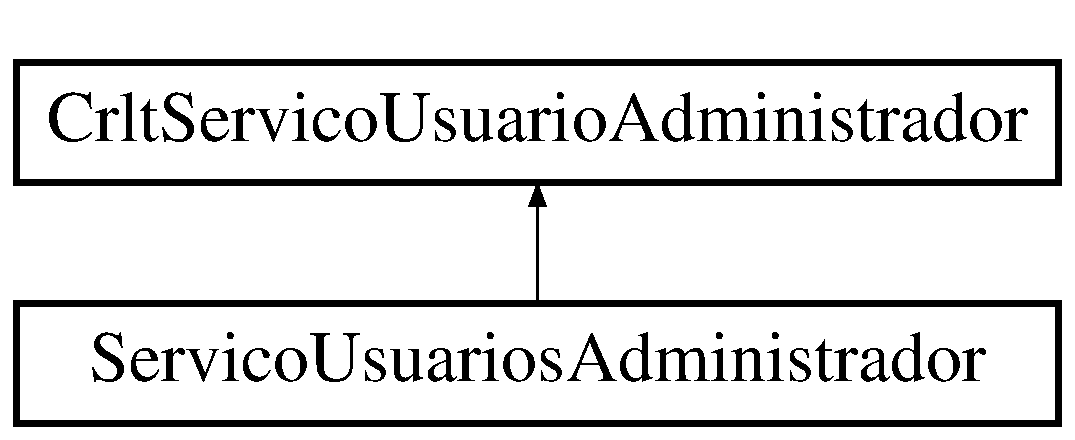
\includegraphics[height=2.000000cm]{class_crlt_servico_usuario_administrador}
\end{center}
\end{figure}
\subsection*{Membros Públicos}
\begin{DoxyCompactItemize}
\item 
virtual void \mbox{\hyperlink{class_crlt_servico_usuario_administrador_af98ebf0c1347a8df6a06e8465312ed3a}{consultar\+Cadastro\+Administrador}} (string email)=0
\item 
virtual void \mbox{\hyperlink{class_crlt_servico_usuario_administrador_ae45ee7ca343542d01898c2919e2671a1}{excluir\+Usuario\+Administrador}} (string email)=0
\item 
virtual void \mbox{\hyperlink{class_crlt_servico_usuario_administrador_ab0492870331c189997ea174f0482202e}{atualizar\+Usuario\+Administrador}} (string email)=0
\item 
virtual void \mbox{\hyperlink{class_crlt_servico_usuario_administrador_ad9ced45046d895a48f1b84b975b89cb1}{list\+Nome\+Vocabularios}} ()=0
\item 
virtual void \mbox{\hyperlink{class_crlt_servico_usuario_administrador_af6b9c9eb9a047c0677de25b07062bff5}{list\+Dados\+Vocabulario}} ()=0
\item 
virtual void \mbox{\hyperlink{class_crlt_servico_usuario_administrador_a6924f2f9e7b9b80ddc1be753628fe989}{consultar\+Termo}} ()=0
\item 
virtual void \mbox{\hyperlink{class_crlt_servico_usuario_administrador_a2cddc1d55c76597e69ce39dab1dc1026}{consultar\+Definicao\+Termo}} ()=0
\item 
virtual void \mbox{\hyperlink{class_crlt_servico_usuario_administrador_ac0432bf5b0788a20f018781bcca74e45}{cadastra\+Desenvolvedor\+Voc\+Controlado}} (string email)=0
\item 
virtual void \mbox{\hyperlink{class_crlt_servico_usuario_administrador_af7c63b86c3ee31bf1a0ae5edca56515c}{cria\+Termo}} ()=0
\item 
virtual void \mbox{\hyperlink{class_crlt_servico_usuario_administrador_a18da82fdae717b90254dbaa003ac14cb}{editar\+Termo}} ()=0
\item 
virtual void \mbox{\hyperlink{class_crlt_servico_usuario_administrador_aa56d5aaff3fcf0dce12f969db7089204}{excluir\+Termo}} ()=0
\item 
virtual void \mbox{\hyperlink{class_crlt_servico_usuario_administrador_a7212381b97babb06c887847980a19d81}{cria\+Definicao}} ()=0
\item 
virtual void \mbox{\hyperlink{class_crlt_servico_usuario_administrador_a37d525a705885131f08e8f74c0926578}{excluir\+Definicao}} ()=0
\item 
virtual void \mbox{\hyperlink{class_crlt_servico_usuario_administrador_a7b709ffa7b27a96970c71997d75b1032}{editar\+Definicao}} ()=0
\item 
virtual void \mbox{\hyperlink{class_crlt_servico_usuario_administrador_a69862854fcbb5cdc3708f39a6aeeea83}{criar\+Vocabulario}} (string email)=0
\item 
virtual void \mbox{\hyperlink{class_crlt_servico_usuario_administrador_aa4ace57c1fe84fc38302133426a2cfd8}{editar\+Def\+Vocabulario}} ()=0
\item 
virtual void \mbox{\hyperlink{class_crlt_servico_usuario_administrador_adf459478defbc327815266343866a1ab}{editar\+Idioma\+Voc}} ()=0
\item 
virtual void \mbox{\hyperlink{class_crlt_servico_usuario_administrador_a55d722de48eb016aef0d7290cb36e51d}{excluir\+Vocabulario}} ()=0
\end{DoxyCompactItemize}


\subsection{Funções membros}
\mbox{\Hypertarget{class_crlt_servico_usuario_administrador_ab0492870331c189997ea174f0482202e}\label{class_crlt_servico_usuario_administrador_ab0492870331c189997ea174f0482202e}} 
\index{Crlt\+Servico\+Usuario\+Administrador@{Crlt\+Servico\+Usuario\+Administrador}!atualizar\+Usuario\+Administrador@{atualizar\+Usuario\+Administrador}}
\index{atualizar\+Usuario\+Administrador@{atualizar\+Usuario\+Administrador}!Crlt\+Servico\+Usuario\+Administrador@{Crlt\+Servico\+Usuario\+Administrador}}
\subsubsection{\texorpdfstring{atualizar\+Usuario\+Administrador()}{atualizarUsuarioAdministrador()}}
{\footnotesize\ttfamily virtual void Crlt\+Servico\+Usuario\+Administrador\+::atualizar\+Usuario\+Administrador (\begin{DoxyParamCaption}\item[{string}]{email }\end{DoxyParamCaption})\hspace{0.3cm}{\ttfamily [pure virtual]}}



Implementado por \mbox{\hyperlink{class_servico_usuarios_administrador_a1111b56d40dff5aa7186c4f3dfe2e598}{Servico\+Usuarios\+Administrador}}.

\mbox{\Hypertarget{class_crlt_servico_usuario_administrador_ac0432bf5b0788a20f018781bcca74e45}\label{class_crlt_servico_usuario_administrador_ac0432bf5b0788a20f018781bcca74e45}} 
\index{Crlt\+Servico\+Usuario\+Administrador@{Crlt\+Servico\+Usuario\+Administrador}!cadastra\+Desenvolvedor\+Voc\+Controlado@{cadastra\+Desenvolvedor\+Voc\+Controlado}}
\index{cadastra\+Desenvolvedor\+Voc\+Controlado@{cadastra\+Desenvolvedor\+Voc\+Controlado}!Crlt\+Servico\+Usuario\+Administrador@{Crlt\+Servico\+Usuario\+Administrador}}
\subsubsection{\texorpdfstring{cadastra\+Desenvolvedor\+Voc\+Controlado()}{cadastraDesenvolvedorVocControlado()}}
{\footnotesize\ttfamily virtual void Crlt\+Servico\+Usuario\+Administrador\+::cadastra\+Desenvolvedor\+Voc\+Controlado (\begin{DoxyParamCaption}\item[{string}]{email }\end{DoxyParamCaption})\hspace{0.3cm}{\ttfamily [pure virtual]}}



Implementado por \mbox{\hyperlink{class_servico_usuarios_administrador_a0a20923a2c556fa62587fac48b6e55da}{Servico\+Usuarios\+Administrador}}.

\mbox{\Hypertarget{class_crlt_servico_usuario_administrador_af98ebf0c1347a8df6a06e8465312ed3a}\label{class_crlt_servico_usuario_administrador_af98ebf0c1347a8df6a06e8465312ed3a}} 
\index{Crlt\+Servico\+Usuario\+Administrador@{Crlt\+Servico\+Usuario\+Administrador}!consultar\+Cadastro\+Administrador@{consultar\+Cadastro\+Administrador}}
\index{consultar\+Cadastro\+Administrador@{consultar\+Cadastro\+Administrador}!Crlt\+Servico\+Usuario\+Administrador@{Crlt\+Servico\+Usuario\+Administrador}}
\subsubsection{\texorpdfstring{consultar\+Cadastro\+Administrador()}{consultarCadastroAdministrador()}}
{\footnotesize\ttfamily virtual void Crlt\+Servico\+Usuario\+Administrador\+::consultar\+Cadastro\+Administrador (\begin{DoxyParamCaption}\item[{string}]{email }\end{DoxyParamCaption})\hspace{0.3cm}{\ttfamily [pure virtual]}}



Implementado por \mbox{\hyperlink{class_servico_usuarios_administrador_ae1474bec1c712ba5640c83f4fe666fc4}{Servico\+Usuarios\+Administrador}}.

\mbox{\Hypertarget{class_crlt_servico_usuario_administrador_a2cddc1d55c76597e69ce39dab1dc1026}\label{class_crlt_servico_usuario_administrador_a2cddc1d55c76597e69ce39dab1dc1026}} 
\index{Crlt\+Servico\+Usuario\+Administrador@{Crlt\+Servico\+Usuario\+Administrador}!consultar\+Definicao\+Termo@{consultar\+Definicao\+Termo}}
\index{consultar\+Definicao\+Termo@{consultar\+Definicao\+Termo}!Crlt\+Servico\+Usuario\+Administrador@{Crlt\+Servico\+Usuario\+Administrador}}
\subsubsection{\texorpdfstring{consultar\+Definicao\+Termo()}{consultarDefinicaoTermo()}}
{\footnotesize\ttfamily virtual void Crlt\+Servico\+Usuario\+Administrador\+::consultar\+Definicao\+Termo (\begin{DoxyParamCaption}{ }\end{DoxyParamCaption})\hspace{0.3cm}{\ttfamily [pure virtual]}}



Implementado por \mbox{\hyperlink{class_servico_usuarios_administrador_acc178ea9b5ed289bde27ca853e874962}{Servico\+Usuarios\+Administrador}}.

\mbox{\Hypertarget{class_crlt_servico_usuario_administrador_a6924f2f9e7b9b80ddc1be753628fe989}\label{class_crlt_servico_usuario_administrador_a6924f2f9e7b9b80ddc1be753628fe989}} 
\index{Crlt\+Servico\+Usuario\+Administrador@{Crlt\+Servico\+Usuario\+Administrador}!consultar\+Termo@{consultar\+Termo}}
\index{consultar\+Termo@{consultar\+Termo}!Crlt\+Servico\+Usuario\+Administrador@{Crlt\+Servico\+Usuario\+Administrador}}
\subsubsection{\texorpdfstring{consultar\+Termo()}{consultarTermo()}}
{\footnotesize\ttfamily virtual void Crlt\+Servico\+Usuario\+Administrador\+::consultar\+Termo (\begin{DoxyParamCaption}{ }\end{DoxyParamCaption})\hspace{0.3cm}{\ttfamily [pure virtual]}}



Implementado por \mbox{\hyperlink{class_servico_usuarios_administrador_aec8b05b7c4a2fb318b6be8f6704d68eb}{Servico\+Usuarios\+Administrador}}.

\mbox{\Hypertarget{class_crlt_servico_usuario_administrador_a7212381b97babb06c887847980a19d81}\label{class_crlt_servico_usuario_administrador_a7212381b97babb06c887847980a19d81}} 
\index{Crlt\+Servico\+Usuario\+Administrador@{Crlt\+Servico\+Usuario\+Administrador}!cria\+Definicao@{cria\+Definicao}}
\index{cria\+Definicao@{cria\+Definicao}!Crlt\+Servico\+Usuario\+Administrador@{Crlt\+Servico\+Usuario\+Administrador}}
\subsubsection{\texorpdfstring{cria\+Definicao()}{criaDefinicao()}}
{\footnotesize\ttfamily virtual void Crlt\+Servico\+Usuario\+Administrador\+::cria\+Definicao (\begin{DoxyParamCaption}{ }\end{DoxyParamCaption})\hspace{0.3cm}{\ttfamily [pure virtual]}}



Implementado por \mbox{\hyperlink{class_servico_usuarios_administrador_a10298cc0f8e8c1b6f44363747bc8de1e}{Servico\+Usuarios\+Administrador}}.

\mbox{\Hypertarget{class_crlt_servico_usuario_administrador_a69862854fcbb5cdc3708f39a6aeeea83}\label{class_crlt_servico_usuario_administrador_a69862854fcbb5cdc3708f39a6aeeea83}} 
\index{Crlt\+Servico\+Usuario\+Administrador@{Crlt\+Servico\+Usuario\+Administrador}!criar\+Vocabulario@{criar\+Vocabulario}}
\index{criar\+Vocabulario@{criar\+Vocabulario}!Crlt\+Servico\+Usuario\+Administrador@{Crlt\+Servico\+Usuario\+Administrador}}
\subsubsection{\texorpdfstring{criar\+Vocabulario()}{criarVocabulario()}}
{\footnotesize\ttfamily virtual void Crlt\+Servico\+Usuario\+Administrador\+::criar\+Vocabulario (\begin{DoxyParamCaption}\item[{string}]{email }\end{DoxyParamCaption})\hspace{0.3cm}{\ttfamily [pure virtual]}}



Implementado por \mbox{\hyperlink{class_servico_usuarios_administrador_a87f2dca2e2b3858f663b4220f357d26f}{Servico\+Usuarios\+Administrador}}.

\mbox{\Hypertarget{class_crlt_servico_usuario_administrador_af7c63b86c3ee31bf1a0ae5edca56515c}\label{class_crlt_servico_usuario_administrador_af7c63b86c3ee31bf1a0ae5edca56515c}} 
\index{Crlt\+Servico\+Usuario\+Administrador@{Crlt\+Servico\+Usuario\+Administrador}!cria\+Termo@{cria\+Termo}}
\index{cria\+Termo@{cria\+Termo}!Crlt\+Servico\+Usuario\+Administrador@{Crlt\+Servico\+Usuario\+Administrador}}
\subsubsection{\texorpdfstring{cria\+Termo()}{criaTermo()}}
{\footnotesize\ttfamily virtual void Crlt\+Servico\+Usuario\+Administrador\+::cria\+Termo (\begin{DoxyParamCaption}{ }\end{DoxyParamCaption})\hspace{0.3cm}{\ttfamily [pure virtual]}}



Implementado por \mbox{\hyperlink{class_servico_usuarios_administrador_a9002054e8a06338e2a380517b6aeb1f7}{Servico\+Usuarios\+Administrador}}.

\mbox{\Hypertarget{class_crlt_servico_usuario_administrador_a7b709ffa7b27a96970c71997d75b1032}\label{class_crlt_servico_usuario_administrador_a7b709ffa7b27a96970c71997d75b1032}} 
\index{Crlt\+Servico\+Usuario\+Administrador@{Crlt\+Servico\+Usuario\+Administrador}!editar\+Definicao@{editar\+Definicao}}
\index{editar\+Definicao@{editar\+Definicao}!Crlt\+Servico\+Usuario\+Administrador@{Crlt\+Servico\+Usuario\+Administrador}}
\subsubsection{\texorpdfstring{editar\+Definicao()}{editarDefinicao()}}
{\footnotesize\ttfamily virtual void Crlt\+Servico\+Usuario\+Administrador\+::editar\+Definicao (\begin{DoxyParamCaption}{ }\end{DoxyParamCaption})\hspace{0.3cm}{\ttfamily [pure virtual]}}



Implementado por \mbox{\hyperlink{class_servico_usuarios_administrador_aa1bda96596ffda5676af7181eaae9466}{Servico\+Usuarios\+Administrador}}.

\mbox{\Hypertarget{class_crlt_servico_usuario_administrador_aa4ace57c1fe84fc38302133426a2cfd8}\label{class_crlt_servico_usuario_administrador_aa4ace57c1fe84fc38302133426a2cfd8}} 
\index{Crlt\+Servico\+Usuario\+Administrador@{Crlt\+Servico\+Usuario\+Administrador}!editar\+Def\+Vocabulario@{editar\+Def\+Vocabulario}}
\index{editar\+Def\+Vocabulario@{editar\+Def\+Vocabulario}!Crlt\+Servico\+Usuario\+Administrador@{Crlt\+Servico\+Usuario\+Administrador}}
\subsubsection{\texorpdfstring{editar\+Def\+Vocabulario()}{editarDefVocabulario()}}
{\footnotesize\ttfamily virtual void Crlt\+Servico\+Usuario\+Administrador\+::editar\+Def\+Vocabulario (\begin{DoxyParamCaption}{ }\end{DoxyParamCaption})\hspace{0.3cm}{\ttfamily [pure virtual]}}



Implementado por \mbox{\hyperlink{class_servico_usuarios_administrador_a57d5f777ed99a006dc2db5cdb0f135b1}{Servico\+Usuarios\+Administrador}}.

\mbox{\Hypertarget{class_crlt_servico_usuario_administrador_adf459478defbc327815266343866a1ab}\label{class_crlt_servico_usuario_administrador_adf459478defbc327815266343866a1ab}} 
\index{Crlt\+Servico\+Usuario\+Administrador@{Crlt\+Servico\+Usuario\+Administrador}!editar\+Idioma\+Voc@{editar\+Idioma\+Voc}}
\index{editar\+Idioma\+Voc@{editar\+Idioma\+Voc}!Crlt\+Servico\+Usuario\+Administrador@{Crlt\+Servico\+Usuario\+Administrador}}
\subsubsection{\texorpdfstring{editar\+Idioma\+Voc()}{editarIdiomaVoc()}}
{\footnotesize\ttfamily virtual void Crlt\+Servico\+Usuario\+Administrador\+::editar\+Idioma\+Voc (\begin{DoxyParamCaption}{ }\end{DoxyParamCaption})\hspace{0.3cm}{\ttfamily [pure virtual]}}



Implementado por \mbox{\hyperlink{class_servico_usuarios_administrador_ac0d400904b25cd30911a446bce66603a}{Servico\+Usuarios\+Administrador}}.

\mbox{\Hypertarget{class_crlt_servico_usuario_administrador_a18da82fdae717b90254dbaa003ac14cb}\label{class_crlt_servico_usuario_administrador_a18da82fdae717b90254dbaa003ac14cb}} 
\index{Crlt\+Servico\+Usuario\+Administrador@{Crlt\+Servico\+Usuario\+Administrador}!editar\+Termo@{editar\+Termo}}
\index{editar\+Termo@{editar\+Termo}!Crlt\+Servico\+Usuario\+Administrador@{Crlt\+Servico\+Usuario\+Administrador}}
\subsubsection{\texorpdfstring{editar\+Termo()}{editarTermo()}}
{\footnotesize\ttfamily virtual void Crlt\+Servico\+Usuario\+Administrador\+::editar\+Termo (\begin{DoxyParamCaption}{ }\end{DoxyParamCaption})\hspace{0.3cm}{\ttfamily [pure virtual]}}



Implementado por \mbox{\hyperlink{class_servico_usuarios_administrador_a219b135060f3a85d996f506474b99f48}{Servico\+Usuarios\+Administrador}}.

\mbox{\Hypertarget{class_crlt_servico_usuario_administrador_a37d525a705885131f08e8f74c0926578}\label{class_crlt_servico_usuario_administrador_a37d525a705885131f08e8f74c0926578}} 
\index{Crlt\+Servico\+Usuario\+Administrador@{Crlt\+Servico\+Usuario\+Administrador}!excluir\+Definicao@{excluir\+Definicao}}
\index{excluir\+Definicao@{excluir\+Definicao}!Crlt\+Servico\+Usuario\+Administrador@{Crlt\+Servico\+Usuario\+Administrador}}
\subsubsection{\texorpdfstring{excluir\+Definicao()}{excluirDefinicao()}}
{\footnotesize\ttfamily virtual void Crlt\+Servico\+Usuario\+Administrador\+::excluir\+Definicao (\begin{DoxyParamCaption}{ }\end{DoxyParamCaption})\hspace{0.3cm}{\ttfamily [pure virtual]}}



Implementado por \mbox{\hyperlink{class_servico_usuarios_administrador_a1c78a37ca8e92725926d3f13299a50b6}{Servico\+Usuarios\+Administrador}}.

\mbox{\Hypertarget{class_crlt_servico_usuario_administrador_aa56d5aaff3fcf0dce12f969db7089204}\label{class_crlt_servico_usuario_administrador_aa56d5aaff3fcf0dce12f969db7089204}} 
\index{Crlt\+Servico\+Usuario\+Administrador@{Crlt\+Servico\+Usuario\+Administrador}!excluir\+Termo@{excluir\+Termo}}
\index{excluir\+Termo@{excluir\+Termo}!Crlt\+Servico\+Usuario\+Administrador@{Crlt\+Servico\+Usuario\+Administrador}}
\subsubsection{\texorpdfstring{excluir\+Termo()}{excluirTermo()}}
{\footnotesize\ttfamily virtual void Crlt\+Servico\+Usuario\+Administrador\+::excluir\+Termo (\begin{DoxyParamCaption}{ }\end{DoxyParamCaption})\hspace{0.3cm}{\ttfamily [pure virtual]}}



Implementado por \mbox{\hyperlink{class_servico_usuarios_administrador_a90abacb7bb051878e6b016d9993733c1}{Servico\+Usuarios\+Administrador}}.

\mbox{\Hypertarget{class_crlt_servico_usuario_administrador_ae45ee7ca343542d01898c2919e2671a1}\label{class_crlt_servico_usuario_administrador_ae45ee7ca343542d01898c2919e2671a1}} 
\index{Crlt\+Servico\+Usuario\+Administrador@{Crlt\+Servico\+Usuario\+Administrador}!excluir\+Usuario\+Administrador@{excluir\+Usuario\+Administrador}}
\index{excluir\+Usuario\+Administrador@{excluir\+Usuario\+Administrador}!Crlt\+Servico\+Usuario\+Administrador@{Crlt\+Servico\+Usuario\+Administrador}}
\subsubsection{\texorpdfstring{excluir\+Usuario\+Administrador()}{excluirUsuarioAdministrador()}}
{\footnotesize\ttfamily virtual void Crlt\+Servico\+Usuario\+Administrador\+::excluir\+Usuario\+Administrador (\begin{DoxyParamCaption}\item[{string}]{email }\end{DoxyParamCaption})\hspace{0.3cm}{\ttfamily [pure virtual]}}



Implementado por \mbox{\hyperlink{class_servico_usuarios_administrador_a1295e808f5e6322a8e329ff711b2b428}{Servico\+Usuarios\+Administrador}}.

\mbox{\Hypertarget{class_crlt_servico_usuario_administrador_a55d722de48eb016aef0d7290cb36e51d}\label{class_crlt_servico_usuario_administrador_a55d722de48eb016aef0d7290cb36e51d}} 
\index{Crlt\+Servico\+Usuario\+Administrador@{Crlt\+Servico\+Usuario\+Administrador}!excluir\+Vocabulario@{excluir\+Vocabulario}}
\index{excluir\+Vocabulario@{excluir\+Vocabulario}!Crlt\+Servico\+Usuario\+Administrador@{Crlt\+Servico\+Usuario\+Administrador}}
\subsubsection{\texorpdfstring{excluir\+Vocabulario()}{excluirVocabulario()}}
{\footnotesize\ttfamily virtual void Crlt\+Servico\+Usuario\+Administrador\+::excluir\+Vocabulario (\begin{DoxyParamCaption}{ }\end{DoxyParamCaption})\hspace{0.3cm}{\ttfamily [pure virtual]}}



Implementado por \mbox{\hyperlink{class_servico_usuarios_administrador_a13237b760df88f3f8a825a5bcd1d7331}{Servico\+Usuarios\+Administrador}}.

\mbox{\Hypertarget{class_crlt_servico_usuario_administrador_af6b9c9eb9a047c0677de25b07062bff5}\label{class_crlt_servico_usuario_administrador_af6b9c9eb9a047c0677de25b07062bff5}} 
\index{Crlt\+Servico\+Usuario\+Administrador@{Crlt\+Servico\+Usuario\+Administrador}!list\+Dados\+Vocabulario@{list\+Dados\+Vocabulario}}
\index{list\+Dados\+Vocabulario@{list\+Dados\+Vocabulario}!Crlt\+Servico\+Usuario\+Administrador@{Crlt\+Servico\+Usuario\+Administrador}}
\subsubsection{\texorpdfstring{list\+Dados\+Vocabulario()}{listDadosVocabulario()}}
{\footnotesize\ttfamily virtual void Crlt\+Servico\+Usuario\+Administrador\+::list\+Dados\+Vocabulario (\begin{DoxyParamCaption}{ }\end{DoxyParamCaption})\hspace{0.3cm}{\ttfamily [pure virtual]}}



Implementado por \mbox{\hyperlink{class_servico_usuarios_administrador_adddc69a01b3ffb101f3a0b5825dde223}{Servico\+Usuarios\+Administrador}}.

\mbox{\Hypertarget{class_crlt_servico_usuario_administrador_ad9ced45046d895a48f1b84b975b89cb1}\label{class_crlt_servico_usuario_administrador_ad9ced45046d895a48f1b84b975b89cb1}} 
\index{Crlt\+Servico\+Usuario\+Administrador@{Crlt\+Servico\+Usuario\+Administrador}!list\+Nome\+Vocabularios@{list\+Nome\+Vocabularios}}
\index{list\+Nome\+Vocabularios@{list\+Nome\+Vocabularios}!Crlt\+Servico\+Usuario\+Administrador@{Crlt\+Servico\+Usuario\+Administrador}}
\subsubsection{\texorpdfstring{list\+Nome\+Vocabularios()}{listNomeVocabularios()}}
{\footnotesize\ttfamily virtual void Crlt\+Servico\+Usuario\+Administrador\+::list\+Nome\+Vocabularios (\begin{DoxyParamCaption}{ }\end{DoxyParamCaption})\hspace{0.3cm}{\ttfamily [pure virtual]}}



Implementado por \mbox{\hyperlink{class_servico_usuarios_administrador_a72b7761474e413704531b3234744d0e0}{Servico\+Usuarios\+Administrador}}.



A documentação para essa classe foi gerada a partir do seguinte arquivo\+:\begin{DoxyCompactItemize}
\item 
/\+Users/amadeulinhares/\+Desktop/\+Trabalho3/\mbox{\hyperlink{interface_8hpp}{interface.\+hpp}}\end{DoxyCompactItemize}

\hypertarget{class_crlt_servico_usuario_desenvolvedor}{}\section{Referência da Classe Crlt\+Servico\+Usuario\+Desenvolvedor}
\label{class_crlt_servico_usuario_desenvolvedor}\index{Crlt\+Servico\+Usuario\+Desenvolvedor@{Crlt\+Servico\+Usuario\+Desenvolvedor}}


{\ttfamily \#include $<$interface.\+hpp$>$}

Diagrama de hierarquia para Crlt\+Servico\+Usuario\+Desenvolvedor\+:\begin{figure}[H]
\begin{center}
\leavevmode
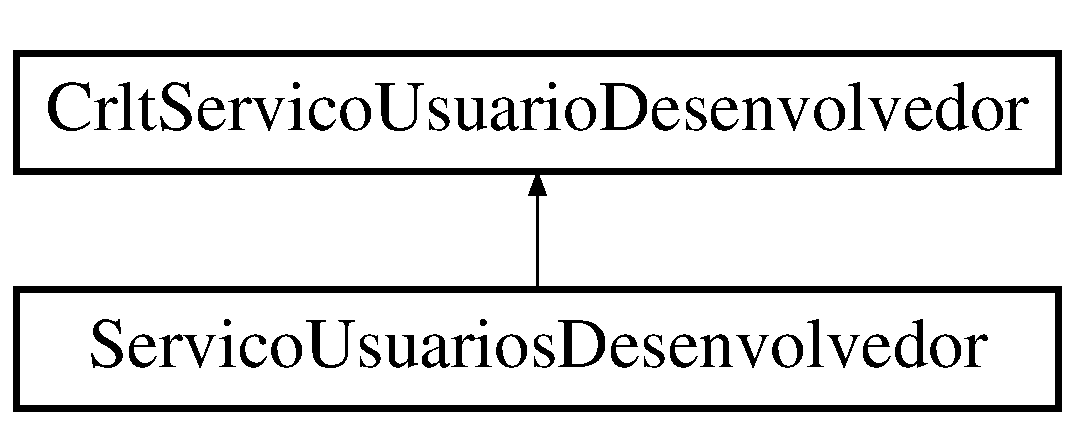
\includegraphics[height=2.000000cm]{class_crlt_servico_usuario_desenvolvedor}
\end{center}
\end{figure}
\subsection*{Membros Públicos}
\begin{DoxyCompactItemize}
\item 
virtual int \mbox{\hyperlink{class_crlt_servico_usuario_desenvolvedor_ad0e0d85a9a4763960f021fca4cf36f29}{consultar\+Cadastro\+Desenvolvedor}} (string email)=0
\item 
virtual void \mbox{\hyperlink{class_crlt_servico_usuario_desenvolvedor_aa106326b5823377bd842b7448e0b4ee3}{excluir\+Usuario\+Desenvolvedor}} (string email)=0
\item 
virtual void \mbox{\hyperlink{class_crlt_servico_usuario_desenvolvedor_a63705805bc01450509e7719e2a57b1da}{atualizar\+Usuario\+Desenvolvedor}} (string email)=0
\item 
virtual void \mbox{\hyperlink{class_crlt_servico_usuario_desenvolvedor_abb3f10c499ac67d02987f0860150393d}{list\+Nome\+Vocabularios}} ()=0
\item 
virtual void \mbox{\hyperlink{class_crlt_servico_usuario_desenvolvedor_a8fb9d062db341aa57ee44ff7b5049652}{list\+Dados\+Vocabulario}} ()=0
\item 
virtual void \mbox{\hyperlink{class_crlt_servico_usuario_desenvolvedor_a328f8ac2978c844ed4331d61ebfce32a}{consultar\+Termo}} ()=0
\item 
virtual void \mbox{\hyperlink{class_crlt_servico_usuario_desenvolvedor_acde5327b99fb4357276c4b0ab83fa20b}{consultar\+Definicao\+Termo}} ()=0
\item 
virtual void \mbox{\hyperlink{class_crlt_servico_usuario_desenvolvedor_a8eb6d3af46ac497a394882ef0fe32eb1}{cadastra\+Desenvolvedor\+Voc\+Controlado}} (string email)=0
\item 
virtual void \mbox{\hyperlink{class_crlt_servico_usuario_desenvolvedor_a924f7dcd059d8ff265909d29457a961b}{cria\+Termo}} ()=0
\item 
virtual void \mbox{\hyperlink{class_crlt_servico_usuario_desenvolvedor_a60098c3dd81dfb83ea03f4b7ace785dc}{editar\+Termo}} ()=0
\item 
virtual void \mbox{\hyperlink{class_crlt_servico_usuario_desenvolvedor_a95825708aeed4c1f6a5829ad4bd29673}{excluir\+Termo}} ()=0
\item 
virtual void \mbox{\hyperlink{class_crlt_servico_usuario_desenvolvedor_af9f1bd8b7ec576adb4bc2a8ac14e0905}{cria\+Definicao}} ()=0
\item 
virtual void \mbox{\hyperlink{class_crlt_servico_usuario_desenvolvedor_a518fe0443e450a73a7274b8dbef74a71}{excluir\+Definicao}} ()=0
\item 
virtual void \mbox{\hyperlink{class_crlt_servico_usuario_desenvolvedor_ae8e2d1d6954d5c4861d3cc40c525f725}{editar\+Definicao}} ()=0
\item 
virtual \mbox{\hyperlink{class_crlt_servico_usuario_desenvolvedor_aa38067f9202f32202dc783e468fd7430}{$\sim$\+Crlt\+Servico\+Usuario\+Desenvolvedor}} ()
\end{DoxyCompactItemize}


\subsection{Construtores e Destrutores}
\mbox{\Hypertarget{class_crlt_servico_usuario_desenvolvedor_aa38067f9202f32202dc783e468fd7430}\label{class_crlt_servico_usuario_desenvolvedor_aa38067f9202f32202dc783e468fd7430}} 
\index{Crlt\+Servico\+Usuario\+Desenvolvedor@{Crlt\+Servico\+Usuario\+Desenvolvedor}!````~Crlt\+Servico\+Usuario\+Desenvolvedor@{$\sim$\+Crlt\+Servico\+Usuario\+Desenvolvedor}}
\index{````~Crlt\+Servico\+Usuario\+Desenvolvedor@{$\sim$\+Crlt\+Servico\+Usuario\+Desenvolvedor}!Crlt\+Servico\+Usuario\+Desenvolvedor@{Crlt\+Servico\+Usuario\+Desenvolvedor}}
\subsubsection{\texorpdfstring{$\sim$\+Crlt\+Servico\+Usuario\+Desenvolvedor()}{~CrltServicoUsuarioDesenvolvedor()}}
{\footnotesize\ttfamily virtual Crlt\+Servico\+Usuario\+Desenvolvedor\+::$\sim$\+Crlt\+Servico\+Usuario\+Desenvolvedor (\begin{DoxyParamCaption}{ }\end{DoxyParamCaption})\hspace{0.3cm}{\ttfamily [inline]}, {\ttfamily [virtual]}}


\begin{DoxyCode}
99 \{\}
\end{DoxyCode}


\subsection{Funções membros}
\mbox{\Hypertarget{class_crlt_servico_usuario_desenvolvedor_a63705805bc01450509e7719e2a57b1da}\label{class_crlt_servico_usuario_desenvolvedor_a63705805bc01450509e7719e2a57b1da}} 
\index{Crlt\+Servico\+Usuario\+Desenvolvedor@{Crlt\+Servico\+Usuario\+Desenvolvedor}!atualizar\+Usuario\+Desenvolvedor@{atualizar\+Usuario\+Desenvolvedor}}
\index{atualizar\+Usuario\+Desenvolvedor@{atualizar\+Usuario\+Desenvolvedor}!Crlt\+Servico\+Usuario\+Desenvolvedor@{Crlt\+Servico\+Usuario\+Desenvolvedor}}
\subsubsection{\texorpdfstring{atualizar\+Usuario\+Desenvolvedor()}{atualizarUsuarioDesenvolvedor()}}
{\footnotesize\ttfamily virtual void Crlt\+Servico\+Usuario\+Desenvolvedor\+::atualizar\+Usuario\+Desenvolvedor (\begin{DoxyParamCaption}\item[{string}]{email }\end{DoxyParamCaption})\hspace{0.3cm}{\ttfamily [pure virtual]}}



Implementado por \mbox{\hyperlink{class_servico_usuarios_desenvolvedor_a2dc1811265f101d3ce14150594b25e88}{Servico\+Usuarios\+Desenvolvedor}}.

\mbox{\Hypertarget{class_crlt_servico_usuario_desenvolvedor_a8eb6d3af46ac497a394882ef0fe32eb1}\label{class_crlt_servico_usuario_desenvolvedor_a8eb6d3af46ac497a394882ef0fe32eb1}} 
\index{Crlt\+Servico\+Usuario\+Desenvolvedor@{Crlt\+Servico\+Usuario\+Desenvolvedor}!cadastra\+Desenvolvedor\+Voc\+Controlado@{cadastra\+Desenvolvedor\+Voc\+Controlado}}
\index{cadastra\+Desenvolvedor\+Voc\+Controlado@{cadastra\+Desenvolvedor\+Voc\+Controlado}!Crlt\+Servico\+Usuario\+Desenvolvedor@{Crlt\+Servico\+Usuario\+Desenvolvedor}}
\subsubsection{\texorpdfstring{cadastra\+Desenvolvedor\+Voc\+Controlado()}{cadastraDesenvolvedorVocControlado()}}
{\footnotesize\ttfamily virtual void Crlt\+Servico\+Usuario\+Desenvolvedor\+::cadastra\+Desenvolvedor\+Voc\+Controlado (\begin{DoxyParamCaption}\item[{string}]{email }\end{DoxyParamCaption})\hspace{0.3cm}{\ttfamily [pure virtual]}}



Implementado por \mbox{\hyperlink{class_servico_usuarios_desenvolvedor_a1708877c02739b2447862b2e2349267d}{Servico\+Usuarios\+Desenvolvedor}}.

\mbox{\Hypertarget{class_crlt_servico_usuario_desenvolvedor_ad0e0d85a9a4763960f021fca4cf36f29}\label{class_crlt_servico_usuario_desenvolvedor_ad0e0d85a9a4763960f021fca4cf36f29}} 
\index{Crlt\+Servico\+Usuario\+Desenvolvedor@{Crlt\+Servico\+Usuario\+Desenvolvedor}!consultar\+Cadastro\+Desenvolvedor@{consultar\+Cadastro\+Desenvolvedor}}
\index{consultar\+Cadastro\+Desenvolvedor@{consultar\+Cadastro\+Desenvolvedor}!Crlt\+Servico\+Usuario\+Desenvolvedor@{Crlt\+Servico\+Usuario\+Desenvolvedor}}
\subsubsection{\texorpdfstring{consultar\+Cadastro\+Desenvolvedor()}{consultarCadastroDesenvolvedor()}}
{\footnotesize\ttfamily virtual int Crlt\+Servico\+Usuario\+Desenvolvedor\+::consultar\+Cadastro\+Desenvolvedor (\begin{DoxyParamCaption}\item[{string}]{email }\end{DoxyParamCaption})\hspace{0.3cm}{\ttfamily [pure virtual]}}



Implementado por \mbox{\hyperlink{class_servico_usuarios_desenvolvedor_a552cca1c14e7c9dd87600062d524ffa8}{Servico\+Usuarios\+Desenvolvedor}}.

\mbox{\Hypertarget{class_crlt_servico_usuario_desenvolvedor_acde5327b99fb4357276c4b0ab83fa20b}\label{class_crlt_servico_usuario_desenvolvedor_acde5327b99fb4357276c4b0ab83fa20b}} 
\index{Crlt\+Servico\+Usuario\+Desenvolvedor@{Crlt\+Servico\+Usuario\+Desenvolvedor}!consultar\+Definicao\+Termo@{consultar\+Definicao\+Termo}}
\index{consultar\+Definicao\+Termo@{consultar\+Definicao\+Termo}!Crlt\+Servico\+Usuario\+Desenvolvedor@{Crlt\+Servico\+Usuario\+Desenvolvedor}}
\subsubsection{\texorpdfstring{consultar\+Definicao\+Termo()}{consultarDefinicaoTermo()}}
{\footnotesize\ttfamily virtual void Crlt\+Servico\+Usuario\+Desenvolvedor\+::consultar\+Definicao\+Termo (\begin{DoxyParamCaption}{ }\end{DoxyParamCaption})\hspace{0.3cm}{\ttfamily [pure virtual]}}



Implementado por \mbox{\hyperlink{class_servico_usuarios_desenvolvedor_aa125405f5b747e4e7bbacebd28934e72}{Servico\+Usuarios\+Desenvolvedor}}.

\mbox{\Hypertarget{class_crlt_servico_usuario_desenvolvedor_a328f8ac2978c844ed4331d61ebfce32a}\label{class_crlt_servico_usuario_desenvolvedor_a328f8ac2978c844ed4331d61ebfce32a}} 
\index{Crlt\+Servico\+Usuario\+Desenvolvedor@{Crlt\+Servico\+Usuario\+Desenvolvedor}!consultar\+Termo@{consultar\+Termo}}
\index{consultar\+Termo@{consultar\+Termo}!Crlt\+Servico\+Usuario\+Desenvolvedor@{Crlt\+Servico\+Usuario\+Desenvolvedor}}
\subsubsection{\texorpdfstring{consultar\+Termo()}{consultarTermo()}}
{\footnotesize\ttfamily virtual void Crlt\+Servico\+Usuario\+Desenvolvedor\+::consultar\+Termo (\begin{DoxyParamCaption}{ }\end{DoxyParamCaption})\hspace{0.3cm}{\ttfamily [pure virtual]}}



Implementado por \mbox{\hyperlink{class_servico_usuarios_desenvolvedor_a9c4a519147798c77d3fb6406f8078b9f}{Servico\+Usuarios\+Desenvolvedor}}.

\mbox{\Hypertarget{class_crlt_servico_usuario_desenvolvedor_af9f1bd8b7ec576adb4bc2a8ac14e0905}\label{class_crlt_servico_usuario_desenvolvedor_af9f1bd8b7ec576adb4bc2a8ac14e0905}} 
\index{Crlt\+Servico\+Usuario\+Desenvolvedor@{Crlt\+Servico\+Usuario\+Desenvolvedor}!cria\+Definicao@{cria\+Definicao}}
\index{cria\+Definicao@{cria\+Definicao}!Crlt\+Servico\+Usuario\+Desenvolvedor@{Crlt\+Servico\+Usuario\+Desenvolvedor}}
\subsubsection{\texorpdfstring{cria\+Definicao()}{criaDefinicao()}}
{\footnotesize\ttfamily virtual void Crlt\+Servico\+Usuario\+Desenvolvedor\+::cria\+Definicao (\begin{DoxyParamCaption}{ }\end{DoxyParamCaption})\hspace{0.3cm}{\ttfamily [pure virtual]}}



Implementado por \mbox{\hyperlink{class_servico_usuarios_desenvolvedor_a851c2a4b054df2a14f66c451f4656d52}{Servico\+Usuarios\+Desenvolvedor}}.

\mbox{\Hypertarget{class_crlt_servico_usuario_desenvolvedor_a924f7dcd059d8ff265909d29457a961b}\label{class_crlt_servico_usuario_desenvolvedor_a924f7dcd059d8ff265909d29457a961b}} 
\index{Crlt\+Servico\+Usuario\+Desenvolvedor@{Crlt\+Servico\+Usuario\+Desenvolvedor}!cria\+Termo@{cria\+Termo}}
\index{cria\+Termo@{cria\+Termo}!Crlt\+Servico\+Usuario\+Desenvolvedor@{Crlt\+Servico\+Usuario\+Desenvolvedor}}
\subsubsection{\texorpdfstring{cria\+Termo()}{criaTermo()}}
{\footnotesize\ttfamily virtual void Crlt\+Servico\+Usuario\+Desenvolvedor\+::cria\+Termo (\begin{DoxyParamCaption}{ }\end{DoxyParamCaption})\hspace{0.3cm}{\ttfamily [pure virtual]}}



Implementado por \mbox{\hyperlink{class_servico_usuarios_desenvolvedor_ab378812b1e6b4d648fb8860cf8444210}{Servico\+Usuarios\+Desenvolvedor}}.

\mbox{\Hypertarget{class_crlt_servico_usuario_desenvolvedor_ae8e2d1d6954d5c4861d3cc40c525f725}\label{class_crlt_servico_usuario_desenvolvedor_ae8e2d1d6954d5c4861d3cc40c525f725}} 
\index{Crlt\+Servico\+Usuario\+Desenvolvedor@{Crlt\+Servico\+Usuario\+Desenvolvedor}!editar\+Definicao@{editar\+Definicao}}
\index{editar\+Definicao@{editar\+Definicao}!Crlt\+Servico\+Usuario\+Desenvolvedor@{Crlt\+Servico\+Usuario\+Desenvolvedor}}
\subsubsection{\texorpdfstring{editar\+Definicao()}{editarDefinicao()}}
{\footnotesize\ttfamily virtual void Crlt\+Servico\+Usuario\+Desenvolvedor\+::editar\+Definicao (\begin{DoxyParamCaption}{ }\end{DoxyParamCaption})\hspace{0.3cm}{\ttfamily [pure virtual]}}



Implementado por \mbox{\hyperlink{class_servico_usuarios_desenvolvedor_a2a1063014d21344c6ec9a101741e5a4e}{Servico\+Usuarios\+Desenvolvedor}}.

\mbox{\Hypertarget{class_crlt_servico_usuario_desenvolvedor_a60098c3dd81dfb83ea03f4b7ace785dc}\label{class_crlt_servico_usuario_desenvolvedor_a60098c3dd81dfb83ea03f4b7ace785dc}} 
\index{Crlt\+Servico\+Usuario\+Desenvolvedor@{Crlt\+Servico\+Usuario\+Desenvolvedor}!editar\+Termo@{editar\+Termo}}
\index{editar\+Termo@{editar\+Termo}!Crlt\+Servico\+Usuario\+Desenvolvedor@{Crlt\+Servico\+Usuario\+Desenvolvedor}}
\subsubsection{\texorpdfstring{editar\+Termo()}{editarTermo()}}
{\footnotesize\ttfamily virtual void Crlt\+Servico\+Usuario\+Desenvolvedor\+::editar\+Termo (\begin{DoxyParamCaption}{ }\end{DoxyParamCaption})\hspace{0.3cm}{\ttfamily [pure virtual]}}



Implementado por \mbox{\hyperlink{class_servico_usuarios_desenvolvedor_afb392520e6ea1209abb42ad0327673e0}{Servico\+Usuarios\+Desenvolvedor}}.

\mbox{\Hypertarget{class_crlt_servico_usuario_desenvolvedor_a518fe0443e450a73a7274b8dbef74a71}\label{class_crlt_servico_usuario_desenvolvedor_a518fe0443e450a73a7274b8dbef74a71}} 
\index{Crlt\+Servico\+Usuario\+Desenvolvedor@{Crlt\+Servico\+Usuario\+Desenvolvedor}!excluir\+Definicao@{excluir\+Definicao}}
\index{excluir\+Definicao@{excluir\+Definicao}!Crlt\+Servico\+Usuario\+Desenvolvedor@{Crlt\+Servico\+Usuario\+Desenvolvedor}}
\subsubsection{\texorpdfstring{excluir\+Definicao()}{excluirDefinicao()}}
{\footnotesize\ttfamily virtual void Crlt\+Servico\+Usuario\+Desenvolvedor\+::excluir\+Definicao (\begin{DoxyParamCaption}{ }\end{DoxyParamCaption})\hspace{0.3cm}{\ttfamily [pure virtual]}}



Implementado por \mbox{\hyperlink{class_servico_usuarios_desenvolvedor_a422f9a3ee77a0d560858c9f7c266b9ee}{Servico\+Usuarios\+Desenvolvedor}}.

\mbox{\Hypertarget{class_crlt_servico_usuario_desenvolvedor_a95825708aeed4c1f6a5829ad4bd29673}\label{class_crlt_servico_usuario_desenvolvedor_a95825708aeed4c1f6a5829ad4bd29673}} 
\index{Crlt\+Servico\+Usuario\+Desenvolvedor@{Crlt\+Servico\+Usuario\+Desenvolvedor}!excluir\+Termo@{excluir\+Termo}}
\index{excluir\+Termo@{excluir\+Termo}!Crlt\+Servico\+Usuario\+Desenvolvedor@{Crlt\+Servico\+Usuario\+Desenvolvedor}}
\subsubsection{\texorpdfstring{excluir\+Termo()}{excluirTermo()}}
{\footnotesize\ttfamily virtual void Crlt\+Servico\+Usuario\+Desenvolvedor\+::excluir\+Termo (\begin{DoxyParamCaption}{ }\end{DoxyParamCaption})\hspace{0.3cm}{\ttfamily [pure virtual]}}



Implementado por \mbox{\hyperlink{class_servico_usuarios_desenvolvedor_a20712917886eaf28a2a9b308d14d7b04}{Servico\+Usuarios\+Desenvolvedor}}.

\mbox{\Hypertarget{class_crlt_servico_usuario_desenvolvedor_aa106326b5823377bd842b7448e0b4ee3}\label{class_crlt_servico_usuario_desenvolvedor_aa106326b5823377bd842b7448e0b4ee3}} 
\index{Crlt\+Servico\+Usuario\+Desenvolvedor@{Crlt\+Servico\+Usuario\+Desenvolvedor}!excluir\+Usuario\+Desenvolvedor@{excluir\+Usuario\+Desenvolvedor}}
\index{excluir\+Usuario\+Desenvolvedor@{excluir\+Usuario\+Desenvolvedor}!Crlt\+Servico\+Usuario\+Desenvolvedor@{Crlt\+Servico\+Usuario\+Desenvolvedor}}
\subsubsection{\texorpdfstring{excluir\+Usuario\+Desenvolvedor()}{excluirUsuarioDesenvolvedor()}}
{\footnotesize\ttfamily virtual void Crlt\+Servico\+Usuario\+Desenvolvedor\+::excluir\+Usuario\+Desenvolvedor (\begin{DoxyParamCaption}\item[{string}]{email }\end{DoxyParamCaption})\hspace{0.3cm}{\ttfamily [pure virtual]}}



Implementado por \mbox{\hyperlink{class_servico_usuarios_desenvolvedor_ad536645995beed517216ed96206ae018}{Servico\+Usuarios\+Desenvolvedor}}.

\mbox{\Hypertarget{class_crlt_servico_usuario_desenvolvedor_a8fb9d062db341aa57ee44ff7b5049652}\label{class_crlt_servico_usuario_desenvolvedor_a8fb9d062db341aa57ee44ff7b5049652}} 
\index{Crlt\+Servico\+Usuario\+Desenvolvedor@{Crlt\+Servico\+Usuario\+Desenvolvedor}!list\+Dados\+Vocabulario@{list\+Dados\+Vocabulario}}
\index{list\+Dados\+Vocabulario@{list\+Dados\+Vocabulario}!Crlt\+Servico\+Usuario\+Desenvolvedor@{Crlt\+Servico\+Usuario\+Desenvolvedor}}
\subsubsection{\texorpdfstring{list\+Dados\+Vocabulario()}{listDadosVocabulario()}}
{\footnotesize\ttfamily virtual void Crlt\+Servico\+Usuario\+Desenvolvedor\+::list\+Dados\+Vocabulario (\begin{DoxyParamCaption}{ }\end{DoxyParamCaption})\hspace{0.3cm}{\ttfamily [pure virtual]}}



Implementado por \mbox{\hyperlink{class_servico_usuarios_desenvolvedor_a5748ea9d0e56ffcad31ad486ecb8b79f}{Servico\+Usuarios\+Desenvolvedor}}.

\mbox{\Hypertarget{class_crlt_servico_usuario_desenvolvedor_abb3f10c499ac67d02987f0860150393d}\label{class_crlt_servico_usuario_desenvolvedor_abb3f10c499ac67d02987f0860150393d}} 
\index{Crlt\+Servico\+Usuario\+Desenvolvedor@{Crlt\+Servico\+Usuario\+Desenvolvedor}!list\+Nome\+Vocabularios@{list\+Nome\+Vocabularios}}
\index{list\+Nome\+Vocabularios@{list\+Nome\+Vocabularios}!Crlt\+Servico\+Usuario\+Desenvolvedor@{Crlt\+Servico\+Usuario\+Desenvolvedor}}
\subsubsection{\texorpdfstring{list\+Nome\+Vocabularios()}{listNomeVocabularios()}}
{\footnotesize\ttfamily virtual void Crlt\+Servico\+Usuario\+Desenvolvedor\+::list\+Nome\+Vocabularios (\begin{DoxyParamCaption}{ }\end{DoxyParamCaption})\hspace{0.3cm}{\ttfamily [pure virtual]}}



Implementado por \mbox{\hyperlink{class_servico_usuarios_desenvolvedor_ad4f1b230cdb25ff8a2b8ae0010e99382}{Servico\+Usuarios\+Desenvolvedor}}.



A documentação para essa classe foi gerada a partir do seguinte arquivo\+:\begin{DoxyCompactItemize}
\item 
/\+Users/amadeulinhares/\+Desktop/\+Trabalho3/\mbox{\hyperlink{interface_8hpp}{interface.\+hpp}}\end{DoxyCompactItemize}

\hypertarget{class_crlt_servico_usuario_leitor}{}\section{Referência da Classe Crlt\+Servico\+Usuario\+Leitor}
\label{class_crlt_servico_usuario_leitor}\index{Crlt\+Servico\+Usuario\+Leitor@{Crlt\+Servico\+Usuario\+Leitor}}


{\ttfamily \#include $<$interface.\+hpp$>$}

Diagrama de hierarquia para Crlt\+Servico\+Usuario\+Leitor\+:\begin{figure}[H]
\begin{center}
\leavevmode
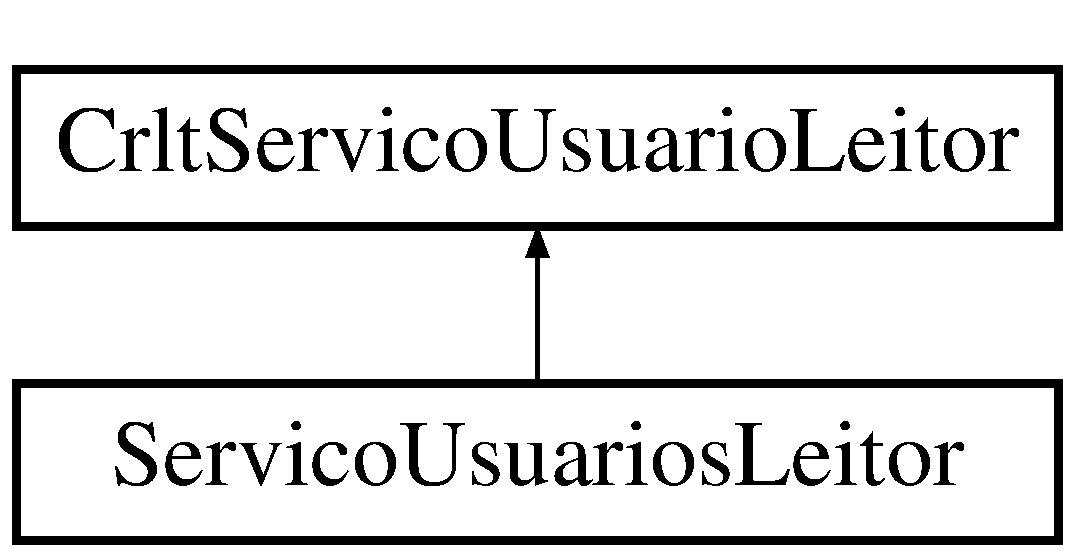
\includegraphics[height=2.000000cm]{class_crlt_servico_usuario_leitor}
\end{center}
\end{figure}
\subsection*{Membros Públicos}
\begin{DoxyCompactItemize}
\item 
virtual int \mbox{\hyperlink{class_crlt_servico_usuario_leitor_a4585305b98f21fe233b2c798edb47496}{consultar\+Cadastro\+Leitor}} (string email)=0
\item 
virtual void \mbox{\hyperlink{class_crlt_servico_usuario_leitor_a8318d7e7dadd648346aeda87fbcd5bca}{excluir\+Usuario\+Leitor}} (string email)=0
\item 
virtual void \mbox{\hyperlink{class_crlt_servico_usuario_leitor_a075822102b4f3cbf1805507d8b78fde8}{atualizar\+Usuario\+Leitor}} (string email)=0
\item 
virtual void \mbox{\hyperlink{class_crlt_servico_usuario_leitor_acfe203ebb5de6884bd4eb5d6167c781f}{list\+Nome\+Vocabularios}} ()=0
\item 
virtual void \mbox{\hyperlink{class_crlt_servico_usuario_leitor_a44a3bc16ef0888d8ce7dd0c9f03fdc58}{list\+Dados\+Vocabulario}} ()=0
\item 
virtual void \mbox{\hyperlink{class_crlt_servico_usuario_leitor_a4b381e72dddde7fffc5a75328dbf3198}{consultar\+Termo}} ()=0
\item 
virtual void \mbox{\hyperlink{class_crlt_servico_usuario_leitor_aefac628815c948981d03e2ad00033b47}{consultar\+Definicao\+Termo}} ()=0
\item 
virtual \mbox{\hyperlink{class_crlt_servico_usuario_leitor_a8d4b033edfd0622f1c82cbd40b2bb293}{$\sim$\+Crlt\+Servico\+Usuario\+Leitor}} ()
\end{DoxyCompactItemize}


\subsection{Construtores e Destrutores}
\mbox{\Hypertarget{class_crlt_servico_usuario_leitor_a8d4b033edfd0622f1c82cbd40b2bb293}\label{class_crlt_servico_usuario_leitor_a8d4b033edfd0622f1c82cbd40b2bb293}} 
\index{Crlt\+Servico\+Usuario\+Leitor@{Crlt\+Servico\+Usuario\+Leitor}!````~Crlt\+Servico\+Usuario\+Leitor@{$\sim$\+Crlt\+Servico\+Usuario\+Leitor}}
\index{````~Crlt\+Servico\+Usuario\+Leitor@{$\sim$\+Crlt\+Servico\+Usuario\+Leitor}!Crlt\+Servico\+Usuario\+Leitor@{Crlt\+Servico\+Usuario\+Leitor}}
\subsubsection{\texorpdfstring{$\sim$\+Crlt\+Servico\+Usuario\+Leitor()}{~CrltServicoUsuarioLeitor()}}
{\footnotesize\ttfamily virtual Crlt\+Servico\+Usuario\+Leitor\+::$\sim$\+Crlt\+Servico\+Usuario\+Leitor (\begin{DoxyParamCaption}{ }\end{DoxyParamCaption})\hspace{0.3cm}{\ttfamily [inline]}, {\ttfamily [virtual]}}


\begin{DoxyCode}
63 \{\}
\end{DoxyCode}


\subsection{Funções membros}
\mbox{\Hypertarget{class_crlt_servico_usuario_leitor_a075822102b4f3cbf1805507d8b78fde8}\label{class_crlt_servico_usuario_leitor_a075822102b4f3cbf1805507d8b78fde8}} 
\index{Crlt\+Servico\+Usuario\+Leitor@{Crlt\+Servico\+Usuario\+Leitor}!atualizar\+Usuario\+Leitor@{atualizar\+Usuario\+Leitor}}
\index{atualizar\+Usuario\+Leitor@{atualizar\+Usuario\+Leitor}!Crlt\+Servico\+Usuario\+Leitor@{Crlt\+Servico\+Usuario\+Leitor}}
\subsubsection{\texorpdfstring{atualizar\+Usuario\+Leitor()}{atualizarUsuarioLeitor()}}
{\footnotesize\ttfamily virtual void Crlt\+Servico\+Usuario\+Leitor\+::atualizar\+Usuario\+Leitor (\begin{DoxyParamCaption}\item[{string}]{email }\end{DoxyParamCaption})\hspace{0.3cm}{\ttfamily [pure virtual]}}



Implementado por \mbox{\hyperlink{class_servico_usuarios_leitor_ad77426aecdda591b99ecbf8259a05b2d}{Servico\+Usuarios\+Leitor}}.

\mbox{\Hypertarget{class_crlt_servico_usuario_leitor_a4585305b98f21fe233b2c798edb47496}\label{class_crlt_servico_usuario_leitor_a4585305b98f21fe233b2c798edb47496}} 
\index{Crlt\+Servico\+Usuario\+Leitor@{Crlt\+Servico\+Usuario\+Leitor}!consultar\+Cadastro\+Leitor@{consultar\+Cadastro\+Leitor}}
\index{consultar\+Cadastro\+Leitor@{consultar\+Cadastro\+Leitor}!Crlt\+Servico\+Usuario\+Leitor@{Crlt\+Servico\+Usuario\+Leitor}}
\subsubsection{\texorpdfstring{consultar\+Cadastro\+Leitor()}{consultarCadastroLeitor()}}
{\footnotesize\ttfamily virtual int Crlt\+Servico\+Usuario\+Leitor\+::consultar\+Cadastro\+Leitor (\begin{DoxyParamCaption}\item[{string}]{email }\end{DoxyParamCaption})\hspace{0.3cm}{\ttfamily [pure virtual]}}



Implementado por \mbox{\hyperlink{class_servico_usuarios_leitor_a8f34dddc0540f729a701d69f948ffb42}{Servico\+Usuarios\+Leitor}}.

\mbox{\Hypertarget{class_crlt_servico_usuario_leitor_aefac628815c948981d03e2ad00033b47}\label{class_crlt_servico_usuario_leitor_aefac628815c948981d03e2ad00033b47}} 
\index{Crlt\+Servico\+Usuario\+Leitor@{Crlt\+Servico\+Usuario\+Leitor}!consultar\+Definicao\+Termo@{consultar\+Definicao\+Termo}}
\index{consultar\+Definicao\+Termo@{consultar\+Definicao\+Termo}!Crlt\+Servico\+Usuario\+Leitor@{Crlt\+Servico\+Usuario\+Leitor}}
\subsubsection{\texorpdfstring{consultar\+Definicao\+Termo()}{consultarDefinicaoTermo()}}
{\footnotesize\ttfamily virtual void Crlt\+Servico\+Usuario\+Leitor\+::consultar\+Definicao\+Termo (\begin{DoxyParamCaption}{ }\end{DoxyParamCaption})\hspace{0.3cm}{\ttfamily [pure virtual]}}



Implementado por \mbox{\hyperlink{class_servico_usuarios_leitor_a89ed39e45ee1c564e1f62df7154d1b29}{Servico\+Usuarios\+Leitor}}.

\mbox{\Hypertarget{class_crlt_servico_usuario_leitor_a4b381e72dddde7fffc5a75328dbf3198}\label{class_crlt_servico_usuario_leitor_a4b381e72dddde7fffc5a75328dbf3198}} 
\index{Crlt\+Servico\+Usuario\+Leitor@{Crlt\+Servico\+Usuario\+Leitor}!consultar\+Termo@{consultar\+Termo}}
\index{consultar\+Termo@{consultar\+Termo}!Crlt\+Servico\+Usuario\+Leitor@{Crlt\+Servico\+Usuario\+Leitor}}
\subsubsection{\texorpdfstring{consultar\+Termo()}{consultarTermo()}}
{\footnotesize\ttfamily virtual void Crlt\+Servico\+Usuario\+Leitor\+::consultar\+Termo (\begin{DoxyParamCaption}{ }\end{DoxyParamCaption})\hspace{0.3cm}{\ttfamily [pure virtual]}}



Implementado por \mbox{\hyperlink{class_servico_usuarios_leitor_a79d3a1814ad33930aae0c3a74c879e92}{Servico\+Usuarios\+Leitor}}.

\mbox{\Hypertarget{class_crlt_servico_usuario_leitor_a8318d7e7dadd648346aeda87fbcd5bca}\label{class_crlt_servico_usuario_leitor_a8318d7e7dadd648346aeda87fbcd5bca}} 
\index{Crlt\+Servico\+Usuario\+Leitor@{Crlt\+Servico\+Usuario\+Leitor}!excluir\+Usuario\+Leitor@{excluir\+Usuario\+Leitor}}
\index{excluir\+Usuario\+Leitor@{excluir\+Usuario\+Leitor}!Crlt\+Servico\+Usuario\+Leitor@{Crlt\+Servico\+Usuario\+Leitor}}
\subsubsection{\texorpdfstring{excluir\+Usuario\+Leitor()}{excluirUsuarioLeitor()}}
{\footnotesize\ttfamily virtual void Crlt\+Servico\+Usuario\+Leitor\+::excluir\+Usuario\+Leitor (\begin{DoxyParamCaption}\item[{string}]{email }\end{DoxyParamCaption})\hspace{0.3cm}{\ttfamily [pure virtual]}}



Implementado por \mbox{\hyperlink{class_servico_usuarios_leitor_adce08fccebc11dbd5f395b8a4bb23d2a}{Servico\+Usuarios\+Leitor}}.

\mbox{\Hypertarget{class_crlt_servico_usuario_leitor_a44a3bc16ef0888d8ce7dd0c9f03fdc58}\label{class_crlt_servico_usuario_leitor_a44a3bc16ef0888d8ce7dd0c9f03fdc58}} 
\index{Crlt\+Servico\+Usuario\+Leitor@{Crlt\+Servico\+Usuario\+Leitor}!list\+Dados\+Vocabulario@{list\+Dados\+Vocabulario}}
\index{list\+Dados\+Vocabulario@{list\+Dados\+Vocabulario}!Crlt\+Servico\+Usuario\+Leitor@{Crlt\+Servico\+Usuario\+Leitor}}
\subsubsection{\texorpdfstring{list\+Dados\+Vocabulario()}{listDadosVocabulario()}}
{\footnotesize\ttfamily virtual void Crlt\+Servico\+Usuario\+Leitor\+::list\+Dados\+Vocabulario (\begin{DoxyParamCaption}{ }\end{DoxyParamCaption})\hspace{0.3cm}{\ttfamily [pure virtual]}}



Implementado por \mbox{\hyperlink{class_servico_usuarios_leitor_a4f533d318634c95d3f756a45c7613047}{Servico\+Usuarios\+Leitor}}.

\mbox{\Hypertarget{class_crlt_servico_usuario_leitor_acfe203ebb5de6884bd4eb5d6167c781f}\label{class_crlt_servico_usuario_leitor_acfe203ebb5de6884bd4eb5d6167c781f}} 
\index{Crlt\+Servico\+Usuario\+Leitor@{Crlt\+Servico\+Usuario\+Leitor}!list\+Nome\+Vocabularios@{list\+Nome\+Vocabularios}}
\index{list\+Nome\+Vocabularios@{list\+Nome\+Vocabularios}!Crlt\+Servico\+Usuario\+Leitor@{Crlt\+Servico\+Usuario\+Leitor}}
\subsubsection{\texorpdfstring{list\+Nome\+Vocabularios()}{listNomeVocabularios()}}
{\footnotesize\ttfamily virtual void Crlt\+Servico\+Usuario\+Leitor\+::list\+Nome\+Vocabularios (\begin{DoxyParamCaption}{ }\end{DoxyParamCaption})\hspace{0.3cm}{\ttfamily [pure virtual]}}



Implementado por \mbox{\hyperlink{class_servico_usuarios_leitor_a376f7cdbdea50d9a01ce611e79d346c4}{Servico\+Usuarios\+Leitor}}.



A documentação para essa classe foi gerada a partir do seguinte arquivo\+:\begin{DoxyCompactItemize}
\item 
/\+Users/amadeulinhares/\+Desktop/\+Trabalho3/\mbox{\hyperlink{interface_8hpp}{interface.\+hpp}}\end{DoxyCompactItemize}

\hypertarget{class_data}{}\section{Referência da Classe Data}
\label{class_data}\index{Data@{Data}}


{\ttfamily \#include $<$dominios.\+hpp$>$}

\subsection*{Membros Públicos}
\begin{DoxyCompactItemize}
\item 
void \mbox{\hyperlink{class_data_a5245638838a033c98a8b760836dddb7d}{set\+Data}} (string data)
\item 
string \mbox{\hyperlink{class_data_afc7b15a5e81334858e48709b2f45cdc3}{get\+Data}} ()
\item 
void \mbox{\hyperlink{class_data_aa3c7b5fcca1f82689a7f6445e4d222c8}{verifica\+Data}} (string data)
\end{DoxyCompactItemize}


\subsection{Descrição detalhada}
D\+E\+C\+L\+A\+R\+A\+C\+AO C\+L\+A\+S\+SE D\+A\+TA 

\subsection{Funções membros}
\mbox{\Hypertarget{class_data_afc7b15a5e81334858e48709b2f45cdc3}\label{class_data_afc7b15a5e81334858e48709b2f45cdc3}} 
\index{Data@{Data}!get\+Data@{get\+Data}}
\index{get\+Data@{get\+Data}!Data@{Data}}
\subsubsection{\texorpdfstring{get\+Data()}{getData()}}
{\footnotesize\ttfamily string Data\+::get\+Data (\begin{DoxyParamCaption}{ }\end{DoxyParamCaption})}


\begin{DoxyCode}
229 \{
230   \textcolor{keywordflow}{return} this->data;
231 \}
\end{DoxyCode}
\mbox{\Hypertarget{class_data_a5245638838a033c98a8b760836dddb7d}\label{class_data_a5245638838a033c98a8b760836dddb7d}} 
\index{Data@{Data}!set\+Data@{set\+Data}}
\index{set\+Data@{set\+Data}!Data@{Data}}
\subsubsection{\texorpdfstring{set\+Data()}{setData()}}
{\footnotesize\ttfamily void Data\+::set\+Data (\begin{DoxyParamCaption}\item[{string}]{data }\end{DoxyParamCaption})}


\begin{DoxyCode}
221 \{
222 
223     \mbox{\hyperlink{class_data_aa3c7b5fcca1f82689a7f6445e4d222c8}{verificaData}}(data);
224     this->data = data;
225 
226 \}
\end{DoxyCode}
\mbox{\Hypertarget{class_data_aa3c7b5fcca1f82689a7f6445e4d222c8}\label{class_data_aa3c7b5fcca1f82689a7f6445e4d222c8}} 
\index{Data@{Data}!verifica\+Data@{verifica\+Data}}
\index{verifica\+Data@{verifica\+Data}!Data@{Data}}
\subsubsection{\texorpdfstring{verifica\+Data()}{verificaData()}}
{\footnotesize\ttfamily void Data\+::verifica\+Data (\begin{DoxyParamCaption}\item[{string}]{data }\end{DoxyParamCaption})}


\begin{DoxyCode}
234 \{
235   \textcolor{keywordtype}{int} tamanho = data.length();
236   \textcolor{keywordflow}{if}(tamanho > 10)
237   \{
238     \textcolor{keywordflow}{throw}\textcolor{stringliteral}{"Erro - Data Invalida\(\backslash\)n"};
239   \}
240 
241   \textcolor{comment}{//verifica mês}
242   \textcolor{keywordtype}{int} dia1 = data[0];
243   \textcolor{keywordtype}{int} dia2 = data[1];
244   \textcolor{keywordtype}{int} mes1 = data[3];
245   \textcolor{keywordtype}{int} mes2 = data[4];
246   \textcolor{keywordtype}{int} ano1 = data[6];
247   \textcolor{keywordtype}{int} ano2 = data[7];
248   \textcolor{keywordtype}{int} ano3 = data[8];
249   \textcolor{keywordtype}{int} ano4 = data[9];
250   \textcolor{keywordtype}{char} teste1 = data[2];
251   \textcolor{keywordtype}{char} teste2 = data[5];
252 
253   \textcolor{keywordflow}{if}(dia1 > 51 || dia2 > 57)
254   \{
255     \textcolor{keywordflow}{throw}\textcolor{stringliteral}{"Erro - Data Invalida\(\backslash\)n"};
256   \}
257 
258   \textcolor{keywordflow}{if}( (mes1 > 49 || mes2 > 50) && (mes1 > 48 || mes2 > 57)  )
259   \{
260     \textcolor{keywordflow}{throw}\textcolor{stringliteral}{"Erro - Data Invalida\(\backslash\)n"};
261   \}
262 
263   \textcolor{keywordflow}{if}( ano1 == 50 )
264   \{
265     \textcolor{keywordflow}{if}( (ano2 != 48) || (ano3 > 57) || (ano4 > 57))
266     \{
267       \textcolor{keywordflow}{throw}\textcolor{stringliteral}{"Erro - Data Invalida\(\backslash\)n"};
268     \}
269   \}
270 
271   \textcolor{keywordflow}{if}(ano1 == 49)
272   \{
273     \textcolor{keywordflow}{if}( (ano2 != 57) || (ano3 < 48) || (ano4 < 48))
274     \{
275       \textcolor{keywordflow}{throw}\textcolor{stringliteral}{"Erro - Data Invalida\(\backslash\)n"};
276     \}
277   \}
278 
279 
280   \textcolor{keywordflow}{if}( (teste1 != \textcolor{charliteral}{'/'}) || ( teste2 != \textcolor{charliteral}{'/'}) )
281   \{
282     \textcolor{keywordflow}{throw}\textcolor{stringliteral}{"Erro - Data Invalida\(\backslash\)n"};
283   \}
284 
285 \}
\end{DoxyCode}


A documentação para essa classe foi gerada a partir dos seguintes arquivos\+:\begin{DoxyCompactItemize}
\item 
/\+Users/amadeulinhares/\+Desktop/\+Trabalho3/\mbox{\hyperlink{dominios_8hpp}{dominios.\+hpp}}\item 
/\+Users/amadeulinhares/\+Desktop/\+Trabalho3/\mbox{\hyperlink{dominios_8cpp}{dominios.\+cpp}}\end{DoxyCompactItemize}

\hypertarget{class_definicao}{}\section{Referência da Classe Definicao}
\label{class_definicao}\index{Definicao@{Definicao}}


{\ttfamily \#include $<$entidades.\+hpp$>$}

\subsection*{Membros Públicos}
\begin{DoxyCompactItemize}
\item 
void \mbox{\hyperlink{class_definicao_a4c4f6ff99c330cde93a0ffb6500489ad}{set\+Texto\+De\+Definicao}} (string texto\+De\+Definicao)
\item 
string \mbox{\hyperlink{class_definicao_accdaa35b92e35e50f62b32265f28c49d}{get\+Texto\+De\+Definicao}} ()
\item 
void \mbox{\hyperlink{class_definicao_a3660abc2f1311be4b88011da6ada736e}{set\+Data}} (const \mbox{\hyperlink{class_data}{Data}} \&data)
\item 
\mbox{\hyperlink{class_data}{Data}} \mbox{\hyperlink{class_definicao_a7f0bbadaa7b23e40fb30c9ee94745c5f}{get\+Data}} ()
\end{DoxyCompactItemize}


\subsection{Descrição detalhada}
D\+E\+C\+L\+A\+R\+A\+C\+AO da classe D\+E\+F\+I\+N\+I\+C\+AO Essa classe possui os atributos que sao objetos\+: \mbox{\hyperlink{class_data}{Data}} Ela diferente das outras possui um novo atributo que nao e um objeto chamado de texto\+De\+Definicao ~\newline
F\+U\+N\+C\+O\+ES E\+N\+T\+I\+D\+A\+DE D\+E\+F\+I\+N\+I\+C\+AO set\+Texto\+De\+Definicao get\+Texto\+De\+Definicao set\+Data get\+Data 

\subsection{Funções membros}
\mbox{\Hypertarget{class_definicao_a7f0bbadaa7b23e40fb30c9ee94745c5f}\label{class_definicao_a7f0bbadaa7b23e40fb30c9ee94745c5f}} 
\index{Definicao@{Definicao}!get\+Data@{get\+Data}}
\index{get\+Data@{get\+Data}!Definicao@{Definicao}}
\subsubsection{\texorpdfstring{get\+Data()}{getData()}}
{\footnotesize\ttfamily \mbox{\hyperlink{class_data}{Data}} Definicao\+::get\+Data (\begin{DoxyParamCaption}{ }\end{DoxyParamCaption})\hspace{0.3cm}{\ttfamily [inline]}}


\begin{DoxyCode}
353 \{
354   \textcolor{keywordflow}{return} data;
355 \}
\end{DoxyCode}
\mbox{\Hypertarget{class_definicao_accdaa35b92e35e50f62b32265f28c49d}\label{class_definicao_accdaa35b92e35e50f62b32265f28c49d}} 
\index{Definicao@{Definicao}!get\+Texto\+De\+Definicao@{get\+Texto\+De\+Definicao}}
\index{get\+Texto\+De\+Definicao@{get\+Texto\+De\+Definicao}!Definicao@{Definicao}}
\subsubsection{\texorpdfstring{get\+Texto\+De\+Definicao()}{getTextoDeDefinicao()}}
{\footnotesize\ttfamily string Definicao\+::get\+Texto\+De\+Definicao (\begin{DoxyParamCaption}{ }\end{DoxyParamCaption})\hspace{0.3cm}{\ttfamily [inline]}}


\begin{DoxyCode}
344 \{
345   \textcolor{keywordflow}{return} textoDeDefinicao;
346 \}
\end{DoxyCode}
\mbox{\Hypertarget{class_definicao_a3660abc2f1311be4b88011da6ada736e}\label{class_definicao_a3660abc2f1311be4b88011da6ada736e}} 
\index{Definicao@{Definicao}!set\+Data@{set\+Data}}
\index{set\+Data@{set\+Data}!Definicao@{Definicao}}
\subsubsection{\texorpdfstring{set\+Data()}{setData()}}
{\footnotesize\ttfamily void Definicao\+::set\+Data (\begin{DoxyParamCaption}\item[{const \mbox{\hyperlink{class_data}{Data}} \&}]{data }\end{DoxyParamCaption})\hspace{0.3cm}{\ttfamily [inline]}}


\begin{DoxyCode}
349 \{
350   this->data = data;
351 \}
\end{DoxyCode}
\mbox{\Hypertarget{class_definicao_a4c4f6ff99c330cde93a0ffb6500489ad}\label{class_definicao_a4c4f6ff99c330cde93a0ffb6500489ad}} 
\index{Definicao@{Definicao}!set\+Texto\+De\+Definicao@{set\+Texto\+De\+Definicao}}
\index{set\+Texto\+De\+Definicao@{set\+Texto\+De\+Definicao}!Definicao@{Definicao}}
\subsubsection{\texorpdfstring{set\+Texto\+De\+Definicao()}{setTextoDeDefinicao()}}
{\footnotesize\ttfamily void Definicao\+::set\+Texto\+De\+Definicao (\begin{DoxyParamCaption}\item[{string}]{texto\+De\+Definicao }\end{DoxyParamCaption})\hspace{0.3cm}{\ttfamily [inline]}}


\begin{DoxyCode}
340 \{
341   this->textoDeDefinicao = textoDeDefinicao;
342 \}
\end{DoxyCode}


A documentação para essa classe foi gerada a partir do seguinte arquivo\+:\begin{DoxyCompactItemize}
\item 
/\+Users/amadeulinhares/\+Desktop/\+Trabalho3/\mbox{\hyperlink{entidades_8hpp}{entidades.\+hpp}}\end{DoxyCompactItemize}

\hypertarget{class_desenvolvedor}{}\section{Referência da Classe Desenvolvedor}
\label{class_desenvolvedor}\index{Desenvolvedor@{Desenvolvedor}}


{\ttfamily \#include $<$entidades.\+hpp$>$}

Diagrama de hierarquia para Desenvolvedor\+:\begin{figure}[H]
\begin{center}
\leavevmode
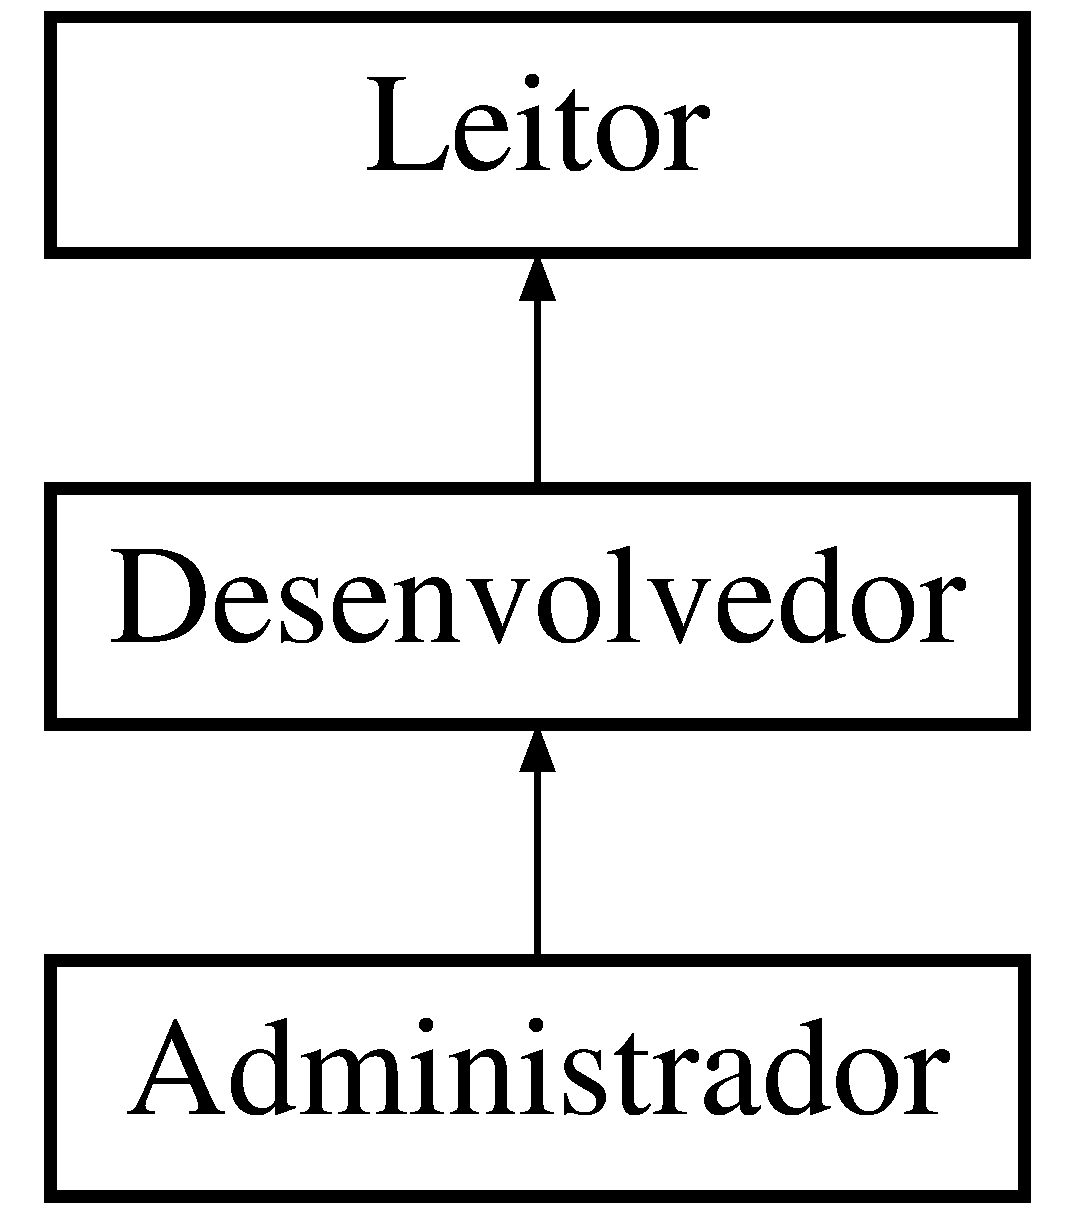
\includegraphics[height=3.000000cm]{class_desenvolvedor}
\end{center}
\end{figure}
\subsection*{Membros Públicos}
\begin{DoxyCompactItemize}
\item 
void \mbox{\hyperlink{class_desenvolvedor_a17ca20f8623c4e3d21676fd7f4b96575}{set\+Data}} (const \mbox{\hyperlink{class_data}{Data}} \&data)
\item 
\mbox{\hyperlink{class_data}{Data}} \mbox{\hyperlink{class_desenvolvedor_ae32b1caacb1a428d29b3e716d648b170}{get\+Data}} ()
\end{DoxyCompactItemize}


\subsection{Descrição detalhada}
D\+E\+C\+L\+A\+R\+A\+C\+AO da classe D\+E\+S\+E\+N\+V\+O\+L\+V\+E\+D\+OR Esta classe herda a classe leitor porem com um atributo a mais O atributo adicionado nessa classe é um objeto do tipo \mbox{\hyperlink{class_data}{Data}} ~\newline
F\+U\+N\+C\+O\+ES E\+N\+T\+I\+D\+A\+DE D\+E\+S\+E\+N\+V\+O\+L\+V\+E\+D\+OR set\+Data get\+Data 

\subsection{Funções membros}
\mbox{\Hypertarget{class_desenvolvedor_ae32b1caacb1a428d29b3e716d648b170}\label{class_desenvolvedor_ae32b1caacb1a428d29b3e716d648b170}} 
\index{Desenvolvedor@{Desenvolvedor}!get\+Data@{get\+Data}}
\index{get\+Data@{get\+Data}!Desenvolvedor@{Desenvolvedor}}
\subsubsection{\texorpdfstring{get\+Data()}{getData()}}
{\footnotesize\ttfamily \mbox{\hyperlink{class_data}{Data}} Desenvolvedor\+::get\+Data (\begin{DoxyParamCaption}{ }\end{DoxyParamCaption})\hspace{0.3cm}{\ttfamily [inline]}}


\begin{DoxyCode}
154   \{
155     \textcolor{keywordflow}{return} data;
156   \}
\end{DoxyCode}
\mbox{\Hypertarget{class_desenvolvedor_a17ca20f8623c4e3d21676fd7f4b96575}\label{class_desenvolvedor_a17ca20f8623c4e3d21676fd7f4b96575}} 
\index{Desenvolvedor@{Desenvolvedor}!set\+Data@{set\+Data}}
\index{set\+Data@{set\+Data}!Desenvolvedor@{Desenvolvedor}}
\subsubsection{\texorpdfstring{set\+Data()}{setData()}}
{\footnotesize\ttfamily void Desenvolvedor\+::set\+Data (\begin{DoxyParamCaption}\item[{const \mbox{\hyperlink{class_data}{Data}} \&}]{data }\end{DoxyParamCaption})\hspace{0.3cm}{\ttfamily [inline]}}


\begin{DoxyCode}
150   \{
151     this->data = data;
152   \}
\end{DoxyCode}


A documentação para essa classe foi gerada a partir do seguinte arquivo\+:\begin{DoxyCompactItemize}
\item 
/\+Users/amadeulinhares/\+Desktop/\+Trabalho3/\mbox{\hyperlink{entidades_8hpp}{entidades.\+hpp}}\end{DoxyCompactItemize}

\hypertarget{class_email}{}\section{Referência da Classe Email}
\label{class_email}\index{Email@{Email}}


{\ttfamily \#include $<$dominios.\+hpp$>$}

\subsection*{Membros Públicos}
\begin{DoxyCompactItemize}
\item 
void \mbox{\hyperlink{class_email_a2614b3a19d961411d1bece9c1bdf616f}{set\+Email}} (string email)
\item 
string \mbox{\hyperlink{class_email_aa9a0e1a66b4efde65cf017bdd1c6c625}{get\+Email}} ()
\item 
void \mbox{\hyperlink{class_email_ab105064f3488d882a3e432052eea954e}{verifica\+Email}} (string email)
\end{DoxyCompactItemize}


\subsection{Descrição detalhada}
D\+E\+C\+L\+A\+R\+A\+C\+AO C\+L\+A\+S\+SE E-\/\+M\+A\+IL 

\subsection{Funções membros}
\mbox{\Hypertarget{class_email_aa9a0e1a66b4efde65cf017bdd1c6c625}\label{class_email_aa9a0e1a66b4efde65cf017bdd1c6c625}} 
\index{Email@{Email}!get\+Email@{get\+Email}}
\index{get\+Email@{get\+Email}!Email@{Email}}
\subsubsection{\texorpdfstring{get\+Email()}{getEmail()}}
{\footnotesize\ttfamily string Email\+::get\+Email (\begin{DoxyParamCaption}{ }\end{DoxyParamCaption})}


\begin{DoxyCode}
298 \{
299   \textcolor{keywordflow}{return} this->email;
300 \}
\end{DoxyCode}
\mbox{\Hypertarget{class_email_a2614b3a19d961411d1bece9c1bdf616f}\label{class_email_a2614b3a19d961411d1bece9c1bdf616f}} 
\index{Email@{Email}!set\+Email@{set\+Email}}
\index{set\+Email@{set\+Email}!Email@{Email}}
\subsubsection{\texorpdfstring{set\+Email()}{setEmail()}}
{\footnotesize\ttfamily void Email\+::set\+Email (\begin{DoxyParamCaption}\item[{string}]{email }\end{DoxyParamCaption})}


\begin{DoxyCode}
291 \{
292   \mbox{\hyperlink{class_email_ab105064f3488d882a3e432052eea954e}{verificaEmail}}(email);
293   this->email = email;
294 
295 \}
\end{DoxyCode}
\mbox{\Hypertarget{class_email_ab105064f3488d882a3e432052eea954e}\label{class_email_ab105064f3488d882a3e432052eea954e}} 
\index{Email@{Email}!verifica\+Email@{verifica\+Email}}
\index{verifica\+Email@{verifica\+Email}!Email@{Email}}
\subsubsection{\texorpdfstring{verifica\+Email()}{verificaEmail()}}
{\footnotesize\ttfamily void Email\+::verifica\+Email (\begin{DoxyParamCaption}\item[{string}]{email }\end{DoxyParamCaption})}


\begin{DoxyCode}
303 \{
304   \textcolor{keywordtype}{int} tamanhoEmail = email.length();
305   \textcolor{keywordtype}{int} verifica = 0;
306   \textcolor{keywordtype}{int} i,z;
307   \textcolor{keywordtype}{char} auxiliar;
308   \textcolor{keywordtype}{int} teste = 0;
309   \textcolor{keywordtype}{int} guardaPosicao;
310 
311   \textcolor{comment}{//verifica se o primeiro nem o ultimo caracter é um ponto}
312   \textcolor{keywordflow}{for}(i = 0 ; i < tamanhoEmail ; i++)
313   \{
314     \textcolor{keywordflow}{if}(email[i] == \textcolor{charliteral}{'@'})
315     \{
316       guardaPosicao = i;
317     \}
318 
319   \}
320 
321   \textcolor{keywordflow}{if}( (email[0] == \textcolor{charliteral}{'.'}) || (email[guardaPosicao - 1] == \textcolor{charliteral}{'.'}) || (email[guardaPosicao + 1] == \textcolor{charliteral}{'-'}) || (email
      [tamanhoEmail - 1] == \textcolor{charliteral}{'-'}) )
322   \{
323     \textcolor{keywordflow}{throw}\textcolor{stringliteral}{"\(\backslash\)nErro: Formato de Email Invalido\(\backslash\)n"};
324 
325   \}
326 
327   \textcolor{comment}{//verifica se existe @ no dominio}
328   \textcolor{keywordflow}{for}(i = 0 ; i < tamanhoEmail ; i++)
329   \{
330     \textcolor{keywordflow}{if}(email[i] == \textcolor{charliteral}{'@'})
331     \{
332       verifica = 1;
333     \}
334 
335   \}
336 
337   \textcolor{keywordflow}{if}(verifica != 1)
338   \{
339     \textcolor{keywordflow}{throw}\textcolor{stringliteral}{"\(\backslash\)nErro: Formato de Email Invalido\(\backslash\)n"};
340 
341   \}
342 
343   \textcolor{comment}{//Verifica se existe letras no dominio}
344   \textcolor{keywordflow}{for}(i = 0 ; i < tamanhoEmail ; i++)
345   \{
346     \textcolor{keywordflow}{if}(email[i] == \textcolor{charliteral}{'@'})
347     \{
348       z = i;
349       \textcolor{keywordflow}{while}(z < tamanhoEmail)
350       \{
351         \textcolor{keywordflow}{if}(isalpha(email[z]))
352         \{
353           teste = 1;
354         \}
355         z++;
356       \}
357     \}
358   \}
359 
360   \textcolor{keywordflow}{if}(teste == 0)
361   \{
362     \textcolor{keywordflow}{throw}\textcolor{stringliteral}{"\(\backslash\)nErro: Formato de Email Invalido\(\backslash\)n"};
363 
364   \}
365 
366 \}
\end{DoxyCode}


A documentação para essa classe foi gerada a partir dos seguintes arquivos\+:\begin{DoxyCompactItemize}
\item 
/\+Users/amadeulinhares/\+Desktop/\+Trabalho3/\mbox{\hyperlink{dominios_8hpp}{dominios.\+hpp}}\item 
/\+Users/amadeulinhares/\+Desktop/\+Trabalho3/\mbox{\hyperlink{dominios_8cpp}{dominios.\+cpp}}\end{DoxyCompactItemize}

\hypertarget{class_endereco}{}\section{Referência da Classe Endereco}
\label{class_endereco}\index{Endereco@{Endereco}}


{\ttfamily \#include $<$dominios.\+hpp$>$}

\subsection*{Membros Públicos}
\begin{DoxyCompactItemize}
\item 
void \mbox{\hyperlink{class_endereco_a36e8c19c5e97f321d77aece5b3e53239}{set\+Endereco}} (string endereco)
\item 
string \mbox{\hyperlink{class_endereco_aa1ccbda52f9559a68379c54e7e914d19}{get\+Endereco}} ()
\end{DoxyCompactItemize}


\subsection{Descrição detalhada}
D\+E\+C\+L\+A\+R\+A\+C\+AO C\+L\+A\+S\+SE E\+N\+D\+E\+R\+E\+CO 

\subsection{Funções membros}
\mbox{\Hypertarget{class_endereco_aa1ccbda52f9559a68379c54e7e914d19}\label{class_endereco_aa1ccbda52f9559a68379c54e7e914d19}} 
\index{Endereco@{Endereco}!get\+Endereco@{get\+Endereco}}
\index{get\+Endereco@{get\+Endereco}!Endereco@{Endereco}}
\subsubsection{\texorpdfstring{get\+Endereco()}{getEndereco()}}
{\footnotesize\ttfamily string Endereco\+::get\+Endereco (\begin{DoxyParamCaption}{ }\end{DoxyParamCaption})}


\begin{DoxyCode}
161 \{
162   \textcolor{keywordflow}{return} this->endereco;
163 \}
\end{DoxyCode}
\mbox{\Hypertarget{class_endereco_a36e8c19c5e97f321d77aece5b3e53239}\label{class_endereco_a36e8c19c5e97f321d77aece5b3e53239}} 
\index{Endereco@{Endereco}!set\+Endereco@{set\+Endereco}}
\index{set\+Endereco@{set\+Endereco}!Endereco@{Endereco}}
\subsubsection{\texorpdfstring{set\+Endereco()}{setEndereco()}}
{\footnotesize\ttfamily void Endereco\+::set\+Endereco (\begin{DoxyParamCaption}\item[{string}]{endereco }\end{DoxyParamCaption})}

Funcoes da classe E\+N\+D\+E\+R\+EÇO set\+Endereco get\+Endereco verifica\+Endereco 
\begin{DoxyCode}
153 \{
154 
155     verificaEndereco(endereco);
156     this->endereco = endereco;
157 
158 \}
\end{DoxyCode}


A documentação para essa classe foi gerada a partir dos seguintes arquivos\+:\begin{DoxyCompactItemize}
\item 
/\+Users/amadeulinhares/\+Desktop/\+Trabalho3/\mbox{\hyperlink{dominios_8hpp}{dominios.\+hpp}}\item 
/\+Users/amadeulinhares/\+Desktop/\+Trabalho3/\mbox{\hyperlink{dominios_8cpp}{dominios.\+cpp}}\end{DoxyCompactItemize}

\hypertarget{class_idioma}{}\section{Referência da Classe Idioma}
\label{class_idioma}\index{Idioma@{Idioma}}


{\ttfamily \#include $<$dominios.\+hpp$>$}

\subsection*{Membros Públicos}
\begin{DoxyCompactItemize}
\item 
void \mbox{\hyperlink{class_idioma_a5c15660dcb0cec1db37a013b990d9895}{set\+Idioma}} (string idioma)
\item 
string \mbox{\hyperlink{class_idioma_ab2f6141eec870d6c40f6ec8d32e68231}{get\+Idioma}} ()
\item 
void \mbox{\hyperlink{class_idioma_a8ea40be7a7fed00c55455009cfc6fc6a}{verifica\+Idioma}} (string idioma)
\end{DoxyCompactItemize}


\subsection{Descrição detalhada}
D\+E\+C\+L\+A\+R\+A\+C\+AO C\+L\+A\+S\+SE I\+D\+I\+O\+MA 

\subsection{Funções membros}
\mbox{\Hypertarget{class_idioma_ab2f6141eec870d6c40f6ec8d32e68231}\label{class_idioma_ab2f6141eec870d6c40f6ec8d32e68231}} 
\index{Idioma@{Idioma}!get\+Idioma@{get\+Idioma}}
\index{get\+Idioma@{get\+Idioma}!Idioma@{Idioma}}
\subsubsection{\texorpdfstring{get\+Idioma()}{getIdioma()}}
{\footnotesize\ttfamily string Idioma\+::get\+Idioma (\begin{DoxyParamCaption}{ }\end{DoxyParamCaption})}


\begin{DoxyCode}
473 \{
474   \textcolor{keywordflow}{return} this->idioma;
475 \}
\end{DoxyCode}
\mbox{\Hypertarget{class_idioma_a5c15660dcb0cec1db37a013b990d9895}\label{class_idioma_a5c15660dcb0cec1db37a013b990d9895}} 
\index{Idioma@{Idioma}!set\+Idioma@{set\+Idioma}}
\index{set\+Idioma@{set\+Idioma}!Idioma@{Idioma}}
\subsubsection{\texorpdfstring{set\+Idioma()}{setIdioma()}}
{\footnotesize\ttfamily void Idioma\+::set\+Idioma (\begin{DoxyParamCaption}\item[{string}]{idioma }\end{DoxyParamCaption})}


\begin{DoxyCode}
467 \{
468   \mbox{\hyperlink{class_idioma_a8ea40be7a7fed00c55455009cfc6fc6a}{verificaIdioma}}(idioma);
469   this->idioma = idioma;
470 \}
\end{DoxyCode}
\mbox{\Hypertarget{class_idioma_a8ea40be7a7fed00c55455009cfc6fc6a}\label{class_idioma_a8ea40be7a7fed00c55455009cfc6fc6a}} 
\index{Idioma@{Idioma}!verifica\+Idioma@{verifica\+Idioma}}
\index{verifica\+Idioma@{verifica\+Idioma}!Idioma@{Idioma}}
\subsubsection{\texorpdfstring{verifica\+Idioma()}{verificaIdioma()}}
{\footnotesize\ttfamily void Idioma\+::verifica\+Idioma (\begin{DoxyParamCaption}\item[{string}]{idioma }\end{DoxyParamCaption})}


\begin{DoxyCode}
478 \{
479   \textcolor{keywordflow}{if}( (idioma != \textcolor{stringliteral}{"ENG"}) && (idioma != \textcolor{stringliteral}{"FRA"}) && (idioma != \textcolor{stringliteral}{"GER"}) && (idioma != \textcolor{stringliteral}{"ITA"}) && (idioma != \textcolor{stringliteral}{"POR"})
       && (idioma != \textcolor{stringliteral}{"SPA"}) )
480   \{
481     \textcolor{keywordflow}{throw}\textcolor{stringliteral}{"Erro: Idioma Invalido\(\backslash\)n Formato correto para Idioma: ENG / FRA / ITA / POR\(\backslash\)n Por favor escolha um
       dos idiomas listados acima\(\backslash\)n"};
482   \}
483 
484 \}
\end{DoxyCode}


A documentação para essa classe foi gerada a partir dos seguintes arquivos\+:\begin{DoxyCompactItemize}
\item 
/\+Users/amadeulinhares/\+Desktop/\+Trabalho3/\mbox{\hyperlink{dominios_8hpp}{dominios.\+hpp}}\item 
/\+Users/amadeulinhares/\+Desktop/\+Trabalho3/\mbox{\hyperlink{dominios_8cpp}{dominios.\+cpp}}\end{DoxyCompactItemize}

\hypertarget{class_leitor}{}\section{Referência da Classe Leitor}
\label{class_leitor}\index{Leitor@{Leitor}}


{\ttfamily \#include $<$entidades.\+hpp$>$}

Diagrama de hierarquia para Leitor\+:\begin{figure}[H]
\begin{center}
\leavevmode
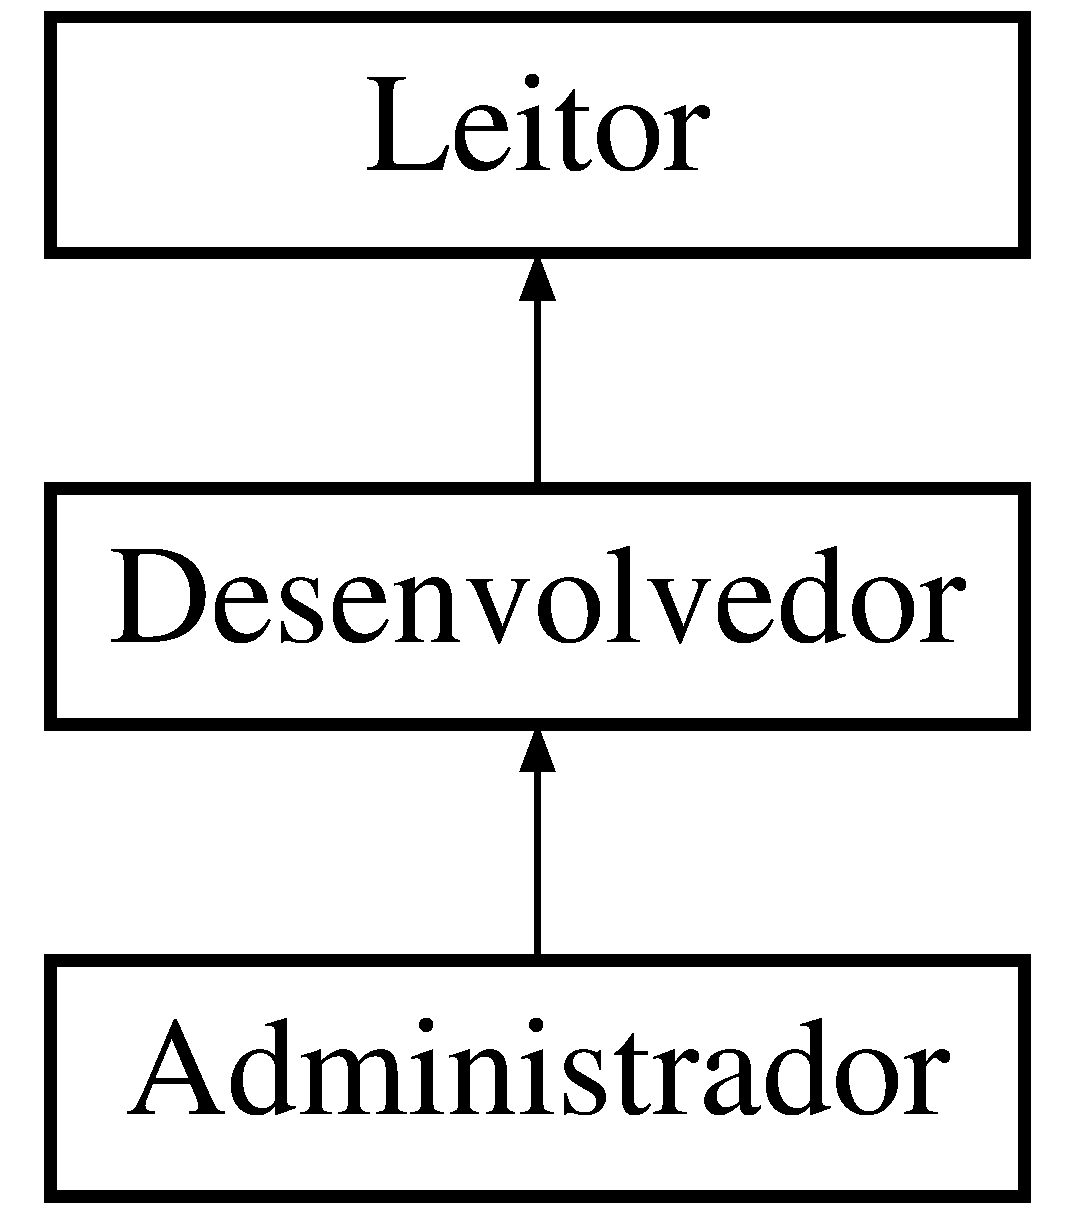
\includegraphics[height=3.000000cm]{class_leitor}
\end{center}
\end{figure}
\subsection*{Membros Públicos}
\begin{DoxyCompactItemize}
\item 
void \mbox{\hyperlink{class_leitor_a2698f4915451a7a53985b8cd275f4ae1}{set\+Nome}} (const \mbox{\hyperlink{class_nome}{Nome}} \&nome)
\item 
\mbox{\hyperlink{class_nome}{Nome}} \mbox{\hyperlink{class_leitor_af12cee66e7318fcbb6a0e407a40fb902}{get\+Nome}} () const
\item 
void \mbox{\hyperlink{class_leitor_affdb7e753343758607242d67dcda033b}{set\+Sobrenome}} (const \mbox{\hyperlink{class_sobrenome}{Sobrenome}} \&sobrenome)
\item 
\mbox{\hyperlink{class_sobrenome}{Sobrenome}} \mbox{\hyperlink{class_leitor_ad8cf5a7cedecd12d087f7dde668c724a}{get\+Sobrenome}} ()
\item 
void \mbox{\hyperlink{class_leitor_adc476ba94b63efc6416c22989e55e7e0}{set\+Email}} (const \mbox{\hyperlink{class_email}{Email}} \&email)
\item 
\mbox{\hyperlink{class_email}{Email}} \mbox{\hyperlink{class_leitor_ae6cd620931ae336b9d9afa4f83944fc1}{get\+Email}} ()
\item 
void \mbox{\hyperlink{class_leitor_a6ddd3a32947bf14f52f1794b5e2d552f}{set\+Senha}} (const \mbox{\hyperlink{class_senha}{Senha}} \&senha)
\item 
\mbox{\hyperlink{class_senha}{Senha}} \mbox{\hyperlink{class_leitor_ae9e88af5c4f0db47e6c19040f7281f2a}{get\+Senha}} ()
\item 
string \mbox{\hyperlink{class_leitor_a013a50e7e5d471efe31ce4f612b7399d}{converte\+Nome}} (string nome)
\item 
string \mbox{\hyperlink{class_leitor_ad18d27138f12d31c4d7d3b011b7d1579}{converte\+Senha}} (string senha)
\item 
void \mbox{\hyperlink{class_leitor_ab3d322a25d04ea7c6b8daf0d1bf0d85f}{valida\+Senha}} (string senha, string nome)
\end{DoxyCompactItemize}


\subsection{Descrição detalhada}
F\+U\+N\+C\+O\+ES E\+N\+T\+I\+D\+A\+DE L\+E\+I\+T\+OR set\+Nome get\+Nome set\+Sobrenome get\+Sobrenome set\+Email get\+Email set\+Senha get\+Senha converte\+Nome converte\+Senha valida\+Senha 

\subsection{Funções membros}
\mbox{\Hypertarget{class_leitor_a013a50e7e5d471efe31ce4f612b7399d}\label{class_leitor_a013a50e7e5d471efe31ce4f612b7399d}} 
\index{Leitor@{Leitor}!converte\+Nome@{converte\+Nome}}
\index{converte\+Nome@{converte\+Nome}!Leitor@{Leitor}}
\subsubsection{\texorpdfstring{converte\+Nome()}{converteNome()}}
{\footnotesize\ttfamily string Leitor\+::converte\+Nome (\begin{DoxyParamCaption}\item[{string}]{nome }\end{DoxyParamCaption})\hspace{0.3cm}{\ttfamily [inline]}}


\begin{DoxyCode}
69 \{
70  \textcolor{keywordflow}{for}(\textcolor{keywordtype}{int} i = 0; i<nome.length(); i++)
71  \{
72    nome[i] = toupper(nome[i]);
73  \}
74 
75  \textcolor{keywordflow}{return} nome;
76 \}
\end{DoxyCode}
\mbox{\Hypertarget{class_leitor_ad18d27138f12d31c4d7d3b011b7d1579}\label{class_leitor_ad18d27138f12d31c4d7d3b011b7d1579}} 
\index{Leitor@{Leitor}!converte\+Senha@{converte\+Senha}}
\index{converte\+Senha@{converte\+Senha}!Leitor@{Leitor}}
\subsubsection{\texorpdfstring{converte\+Senha()}{converteSenha()}}
{\footnotesize\ttfamily string Leitor\+::converte\+Senha (\begin{DoxyParamCaption}\item[{string}]{senha }\end{DoxyParamCaption})\hspace{0.3cm}{\ttfamily [inline]}}


\begin{DoxyCode}
79 \{
80  \textcolor{keywordflow}{for}(\textcolor{keywordtype}{int} i = 0; i<senha.length(); i++)
81  \{
82    senha[i] = toupper(senha[i]);
83  \}
84 
85  \textcolor{keywordflow}{return} senha;
86 \}
\end{DoxyCode}
\mbox{\Hypertarget{class_leitor_ae6cd620931ae336b9d9afa4f83944fc1}\label{class_leitor_ae6cd620931ae336b9d9afa4f83944fc1}} 
\index{Leitor@{Leitor}!get\+Email@{get\+Email}}
\index{get\+Email@{get\+Email}!Leitor@{Leitor}}
\subsubsection{\texorpdfstring{get\+Email()}{getEmail()}}
{\footnotesize\ttfamily \mbox{\hyperlink{class_email}{Email}} Leitor\+::get\+Email (\begin{DoxyParamCaption}{ }\end{DoxyParamCaption})\hspace{0.3cm}{\ttfamily [inline]}}


\begin{DoxyCode}
54  \{
55    \textcolor{keywordflow}{return} email;
56  \}
\end{DoxyCode}
\mbox{\Hypertarget{class_leitor_af12cee66e7318fcbb6a0e407a40fb902}\label{class_leitor_af12cee66e7318fcbb6a0e407a40fb902}} 
\index{Leitor@{Leitor}!get\+Nome@{get\+Nome}}
\index{get\+Nome@{get\+Nome}!Leitor@{Leitor}}
\subsubsection{\texorpdfstring{get\+Nome()}{getNome()}}
{\footnotesize\ttfamily \mbox{\hyperlink{class_nome}{Nome}} Leitor\+::get\+Nome (\begin{DoxyParamCaption}{ }\end{DoxyParamCaption}) const\hspace{0.3cm}{\ttfamily [inline]}}


\begin{DoxyCode}
34                          \{
35         \textcolor{keywordflow}{return} nome;
36     \}
\end{DoxyCode}
\mbox{\Hypertarget{class_leitor_ae9e88af5c4f0db47e6c19040f7281f2a}\label{class_leitor_ae9e88af5c4f0db47e6c19040f7281f2a}} 
\index{Leitor@{Leitor}!get\+Senha@{get\+Senha}}
\index{get\+Senha@{get\+Senha}!Leitor@{Leitor}}
\subsubsection{\texorpdfstring{get\+Senha()}{getSenha()}}
{\footnotesize\ttfamily \mbox{\hyperlink{class_senha}{Senha}} Leitor\+::get\+Senha (\begin{DoxyParamCaption}{ }\end{DoxyParamCaption})\hspace{0.3cm}{\ttfamily [inline]}}


\begin{DoxyCode}
64 \{
65  \textcolor{keywordflow}{return} senha;
66 \}
\end{DoxyCode}
\mbox{\Hypertarget{class_leitor_ad8cf5a7cedecd12d087f7dde668c724a}\label{class_leitor_ad8cf5a7cedecd12d087f7dde668c724a}} 
\index{Leitor@{Leitor}!get\+Sobrenome@{get\+Sobrenome}}
\index{get\+Sobrenome@{get\+Sobrenome}!Leitor@{Leitor}}
\subsubsection{\texorpdfstring{get\+Sobrenome()}{getSobrenome()}}
{\footnotesize\ttfamily \mbox{\hyperlink{class_sobrenome}{Sobrenome}} Leitor\+::get\+Sobrenome (\begin{DoxyParamCaption}{ }\end{DoxyParamCaption})\hspace{0.3cm}{\ttfamily [inline]}}


\begin{DoxyCode}
44    \{
45      \textcolor{keywordflow}{return} sobrenome;
46    \}
\end{DoxyCode}
\mbox{\Hypertarget{class_leitor_adc476ba94b63efc6416c22989e55e7e0}\label{class_leitor_adc476ba94b63efc6416c22989e55e7e0}} 
\index{Leitor@{Leitor}!set\+Email@{set\+Email}}
\index{set\+Email@{set\+Email}!Leitor@{Leitor}}
\subsubsection{\texorpdfstring{set\+Email()}{setEmail()}}
{\footnotesize\ttfamily void Leitor\+::set\+Email (\begin{DoxyParamCaption}\item[{const \mbox{\hyperlink{class_email}{Email}} \&}]{email }\end{DoxyParamCaption})\hspace{0.3cm}{\ttfamily [inline]}}


\begin{DoxyCode}
49   \{
50     this->email = email;
51   \}
\end{DoxyCode}
\mbox{\Hypertarget{class_leitor_a2698f4915451a7a53985b8cd275f4ae1}\label{class_leitor_a2698f4915451a7a53985b8cd275f4ae1}} 
\index{Leitor@{Leitor}!set\+Nome@{set\+Nome}}
\index{set\+Nome@{set\+Nome}!Leitor@{Leitor}}
\subsubsection{\texorpdfstring{set\+Nome()}{setNome()}}
{\footnotesize\ttfamily void Leitor\+::set\+Nome (\begin{DoxyParamCaption}\item[{const \mbox{\hyperlink{class_nome}{Nome}} \&}]{nome }\end{DoxyParamCaption})\hspace{0.3cm}{\ttfamily [inline]}}


\begin{DoxyCode}
30                                   \{
31         this->nome = nome;
32     \}
\end{DoxyCode}
\mbox{\Hypertarget{class_leitor_a6ddd3a32947bf14f52f1794b5e2d552f}\label{class_leitor_a6ddd3a32947bf14f52f1794b5e2d552f}} 
\index{Leitor@{Leitor}!set\+Senha@{set\+Senha}}
\index{set\+Senha@{set\+Senha}!Leitor@{Leitor}}
\subsubsection{\texorpdfstring{set\+Senha()}{setSenha()}}
{\footnotesize\ttfamily void Leitor\+::set\+Senha (\begin{DoxyParamCaption}\item[{const \mbox{\hyperlink{class_senha}{Senha}} \&}]{senha }\end{DoxyParamCaption})\hspace{0.3cm}{\ttfamily [inline]}}


\begin{DoxyCode}
59 \{
60   this->senha = senha;
61 \}
\end{DoxyCode}
\mbox{\Hypertarget{class_leitor_affdb7e753343758607242d67dcda033b}\label{class_leitor_affdb7e753343758607242d67dcda033b}} 
\index{Leitor@{Leitor}!set\+Sobrenome@{set\+Sobrenome}}
\index{set\+Sobrenome@{set\+Sobrenome}!Leitor@{Leitor}}
\subsubsection{\texorpdfstring{set\+Sobrenome()}{setSobrenome()}}
{\footnotesize\ttfamily void Leitor\+::set\+Sobrenome (\begin{DoxyParamCaption}\item[{const \mbox{\hyperlink{class_sobrenome}{Sobrenome}} \&}]{sobrenome }\end{DoxyParamCaption})\hspace{0.3cm}{\ttfamily [inline]}}


\begin{DoxyCode}
39     \{
40       this->sobrenome = sobrenome;
41     \}
\end{DoxyCode}
\mbox{\Hypertarget{class_leitor_ab3d322a25d04ea7c6b8daf0d1bf0d85f}\label{class_leitor_ab3d322a25d04ea7c6b8daf0d1bf0d85f}} 
\index{Leitor@{Leitor}!valida\+Senha@{valida\+Senha}}
\index{valida\+Senha@{valida\+Senha}!Leitor@{Leitor}}
\subsubsection{\texorpdfstring{valida\+Senha()}{validaSenha()}}
{\footnotesize\ttfamily void Leitor\+::valida\+Senha (\begin{DoxyParamCaption}\item[{string}]{senha,  }\item[{string}]{nome }\end{DoxyParamCaption})\hspace{0.3cm}{\ttfamily [inline]}}


\begin{DoxyCode}
89 \{
90  \textcolor{keywordtype}{string} senhaConvertida = \mbox{\hyperlink{class_leitor_ad18d27138f12d31c4d7d3b011b7d1579}{converteSenha}}(senha);
91  \textcolor{keywordtype}{string} nomeConvertido = \mbox{\hyperlink{class_leitor_a013a50e7e5d471efe31ce4f612b7399d}{converteNome}}(nome);
92  \textcolor{keywordtype}{int} tamanhoNome;
93  \textcolor{keywordtype}{int} i;
94  tamanhoNome = nomeConvertido.length();
95  \textcolor{keywordtype}{string} copiaNome;
96  \textcolor{keywordtype}{int} posicaoNome = senhaConvertida.find(nomeConvertido);
97  \textcolor{keywordtype}{int} t = posicaoNome;
98  \textcolor{keywordtype}{int} verifica = 0;
99 
100  \textcolor{keywordflow}{for}(i = 0 ; i < tamanhoNome ; i++)
101  \{
102    copiaNome[i] = senhaConvertida[t];
103    t++;
104  \}
105 
106  \textcolor{keywordflow}{for}(i = 0 ; i < tamanhoNome ; i++)
107  \{
108 
109    \textcolor{keywordflow}{if}(copiaNome[i] == nomeConvertido[i])
110    \{
111      verifica++;
112    \}
113  \}
114 
115  \textcolor{keywordflow}{if}(verifica == tamanhoNome)
116  \{
117    \textcolor{keywordflow}{throw}\textcolor{stringliteral}{"Senha invalida, seu nome esta contido na senha\(\backslash\)n"};
118  \}
119 
120  cout<<\textcolor{stringliteral}{"Senha Validada com sucesso\(\backslash\)n"};
121 
122 \}
\end{DoxyCode}


A documentação para essa classe foi gerada a partir do seguinte arquivo\+:\begin{DoxyCompactItemize}
\item 
/\+Users/amadeulinhares/\+Desktop/\+Trabalho3/\mbox{\hyperlink{entidades_8hpp}{entidades.\+hpp}}\end{DoxyCompactItemize}

\hypertarget{class_nome}{}\section{Referência da Classe Nome}
\label{class_nome}\index{Nome@{Nome}}


{\ttfamily \#include $<$dominios.\+hpp$>$}

\subsection*{Membros Públicos}
\begin{DoxyCompactItemize}
\item 
void \mbox{\hyperlink{class_nome_a83b9f56ec9f86f4b976846f4c5c65b30}{set\+Nome}} (string nome)
\item 
string \mbox{\hyperlink{class_nome_aad41176173eec20cbbae1576447a3697}{get\+Nome}} ()
\end{DoxyCompactItemize}


\subsection{Descrição detalhada}
D\+E\+C\+L\+A\+R\+A\+C\+AO C\+L\+A\+S\+SE N\+O\+ME 

\subsection{Funções membros}
\mbox{\Hypertarget{class_nome_aad41176173eec20cbbae1576447a3697}\label{class_nome_aad41176173eec20cbbae1576447a3697}} 
\index{Nome@{Nome}!get\+Nome@{get\+Nome}}
\index{get\+Nome@{get\+Nome}!Nome@{Nome}}
\subsubsection{\texorpdfstring{get\+Nome()}{getNome()}}
{\footnotesize\ttfamily string Nome\+::get\+Nome (\begin{DoxyParamCaption}{ }\end{DoxyParamCaption})}


\begin{DoxyCode}
18 \{
19   \textcolor{keywordflow}{return} this->nome;
20 \}
\end{DoxyCode}
\mbox{\Hypertarget{class_nome_a83b9f56ec9f86f4b976846f4c5c65b30}\label{class_nome_a83b9f56ec9f86f4b976846f4c5c65b30}} 
\index{Nome@{Nome}!set\+Nome@{set\+Nome}}
\index{set\+Nome@{set\+Nome}!Nome@{Nome}}
\subsubsection{\texorpdfstring{set\+Nome()}{setNome()}}
{\footnotesize\ttfamily void Nome\+::set\+Nome (\begin{DoxyParamCaption}\item[{string}]{nome }\end{DoxyParamCaption})}

funcoes da classe N\+O\+ME set\+Nome get\+Nome verifica\+Nome 
\begin{DoxyCode}
11 \{
12     verificaNome(nome);
13     this->nome = nome;
14 
15 \}
\end{DoxyCode}


A documentação para essa classe foi gerada a partir dos seguintes arquivos\+:\begin{DoxyCompactItemize}
\item 
/\+Users/amadeulinhares/\+Desktop/\+Trabalho3/\mbox{\hyperlink{dominios_8hpp}{dominios.\+hpp}}\item 
/\+Users/amadeulinhares/\+Desktop/\+Trabalho3/\mbox{\hyperlink{dominios_8cpp}{dominios.\+cpp}}\end{DoxyCompactItemize}

\hypertarget{class_senha}{}\section{Referência da Classe Senha}
\label{class_senha}\index{Senha@{Senha}}


{\ttfamily \#include $<$dominios.\+hpp$>$}

\subsection*{Membros Públicos}
\begin{DoxyCompactItemize}
\item 
void \mbox{\hyperlink{class_senha_a01bbc2a82c5f405b68f33fe0dc538ec1}{set\+Senha}} (string senha, \mbox{\hyperlink{class_nome}{Nome}} $\ast$nome)
\item 
string \mbox{\hyperlink{class_senha_a8786b3d03b1652e73df1cdce46cbbaaf}{get\+Senha}} ()
\item 
string \mbox{\hyperlink{class_senha_a39b73424d487b79e150b97400585e78b}{converte\+Nome}} (string nome)
\item 
string \mbox{\hyperlink{class_senha_a64d982211a22299b77487531bdc18e1f}{converte\+Senha}} (string senha)
\item 
void \mbox{\hyperlink{class_senha_a5c87578fbe77800cee8c8f51d7a06d17}{valida\+Senha}} (string senha, string nome)
\end{DoxyCompactItemize}


\subsection{Descrição detalhada}
D\+E\+C\+L\+A\+R\+A\+C\+AO C\+L\+A\+S\+SE S\+E\+N\+HA 

\subsection{Funções membros}
\mbox{\Hypertarget{class_senha_a39b73424d487b79e150b97400585e78b}\label{class_senha_a39b73424d487b79e150b97400585e78b}} 
\index{Senha@{Senha}!converte\+Nome@{converte\+Nome}}
\index{converte\+Nome@{converte\+Nome}!Senha@{Senha}}
\subsubsection{\texorpdfstring{converte\+Nome()}{converteNome()}}
{\footnotesize\ttfamily string Senha\+::converte\+Nome (\begin{DoxyParamCaption}\item[{string}]{nome }\end{DoxyParamCaption})}


\begin{DoxyCode}
385 \{
386  \textcolor{keywordflow}{for}(\textcolor{keywordtype}{int} i = 0; i<nome.length(); i++)
387  \{
388    nome[i] = toupper(nome[i]);
389  \}
390 
391  \textcolor{keywordflow}{return} nome;
392 \}
\end{DoxyCode}
\mbox{\Hypertarget{class_senha_a64d982211a22299b77487531bdc18e1f}\label{class_senha_a64d982211a22299b77487531bdc18e1f}} 
\index{Senha@{Senha}!converte\+Senha@{converte\+Senha}}
\index{converte\+Senha@{converte\+Senha}!Senha@{Senha}}
\subsubsection{\texorpdfstring{converte\+Senha()}{converteSenha()}}
{\footnotesize\ttfamily string Senha\+::converte\+Senha (\begin{DoxyParamCaption}\item[{string}]{senha }\end{DoxyParamCaption})}


\begin{DoxyCode}
395 \{
396  \textcolor{keywordflow}{for}(\textcolor{keywordtype}{int} i = 0; i<senha.length(); i++)
397  \{
398    senha[i] = toupper(senha[i]);
399  \}
400 
401  \textcolor{keywordflow}{return} senha;
402 \}
\end{DoxyCode}
\mbox{\Hypertarget{class_senha_a8786b3d03b1652e73df1cdce46cbbaaf}\label{class_senha_a8786b3d03b1652e73df1cdce46cbbaaf}} 
\index{Senha@{Senha}!get\+Senha@{get\+Senha}}
\index{get\+Senha@{get\+Senha}!Senha@{Senha}}
\subsubsection{\texorpdfstring{get\+Senha()}{getSenha()}}
{\footnotesize\ttfamily string Senha\+::get\+Senha (\begin{DoxyParamCaption}{ }\end{DoxyParamCaption})}


\begin{DoxyCode}
379 \{
380   \textcolor{keywordflow}{return} this->senha;
381 \}
\end{DoxyCode}
\mbox{\Hypertarget{class_senha_a01bbc2a82c5f405b68f33fe0dc538ec1}\label{class_senha_a01bbc2a82c5f405b68f33fe0dc538ec1}} 
\index{Senha@{Senha}!set\+Senha@{set\+Senha}}
\index{set\+Senha@{set\+Senha}!Senha@{Senha}}
\subsubsection{\texorpdfstring{set\+Senha()}{setSenha()}}
{\footnotesize\ttfamily void Senha\+::set\+Senha (\begin{DoxyParamCaption}\item[{string}]{senha,  }\item[{\mbox{\hyperlink{class_nome}{Nome}} $\ast$}]{nome }\end{DoxyParamCaption})}


\begin{DoxyCode}
371 \{
372 
373     \mbox{\hyperlink{class_senha_a5c87578fbe77800cee8c8f51d7a06d17}{validaSenha}}(senha,nome->\mbox{\hyperlink{class_nome_aad41176173eec20cbbae1576447a3697}{getNome}}());
374     this->senha = senha;
375 
376 \}
\end{DoxyCode}
\mbox{\Hypertarget{class_senha_a5c87578fbe77800cee8c8f51d7a06d17}\label{class_senha_a5c87578fbe77800cee8c8f51d7a06d17}} 
\index{Senha@{Senha}!valida\+Senha@{valida\+Senha}}
\index{valida\+Senha@{valida\+Senha}!Senha@{Senha}}
\subsubsection{\texorpdfstring{valida\+Senha()}{validaSenha()}}
{\footnotesize\ttfamily void Senha\+::valida\+Senha (\begin{DoxyParamCaption}\item[{string}]{senha,  }\item[{string}]{nome }\end{DoxyParamCaption})}


\begin{DoxyCode}
405 \{
406  \textcolor{keywordtype}{string} senhaConvertida = \mbox{\hyperlink{class_senha_a64d982211a22299b77487531bdc18e1f}{converteSenha}}(senha);
407  \textcolor{keywordtype}{string} nomeConvertido = \mbox{\hyperlink{class_senha_a39b73424d487b79e150b97400585e78b}{converteNome}}(nome);
408  \textcolor{keywordtype}{int} tamanhoNome;
409  \textcolor{keywordtype}{int} i;
410  tamanhoNome = nomeConvertido.length();
411  \textcolor{keywordtype}{string} copiaNome;
412  \textcolor{keywordtype}{int} posicaoNome = senhaConvertida.find(nomeConvertido);
413  \textcolor{keywordtype}{int} t = posicaoNome;
414  \textcolor{keywordtype}{int} verifica = 0;
415 
416  \textcolor{keywordflow}{for}(i = 0 ; i < tamanhoNome ; i++)
417  \{
418    copiaNome[i] = senhaConvertida[t];
419    t++;
420  \}
421 
422  \textcolor{keywordflow}{for}(i = 0 ; i < tamanhoNome ; i++)
423  \{
424 
425    \textcolor{keywordflow}{if}(copiaNome[i] == nomeConvertido[i])
426    \{
427      verifica++;
428    \}
429  \}
430 
431  \textcolor{keywordflow}{if}(verifica == tamanhoNome)
432  \{
433    \textcolor{keywordflow}{throw}\textcolor{stringliteral}{"\(\backslash\)nSenha invalida, seu nome esta contido na senha\(\backslash\)n"};
434  \}
435 
436  cout<<\textcolor{stringliteral}{"\(\backslash\)nSenha Validada com sucesso\(\backslash\)n"};
437 
438 \}
\end{DoxyCode}


A documentação para essa classe foi gerada a partir dos seguintes arquivos\+:\begin{DoxyCompactItemize}
\item 
/\+Users/amadeulinhares/\+Desktop/\+Trabalho3/\mbox{\hyperlink{dominios_8hpp}{dominios.\+hpp}}\item 
/\+Users/amadeulinhares/\+Desktop/\+Trabalho3/\mbox{\hyperlink{dominios_8cpp}{dominios.\+cpp}}\end{DoxyCompactItemize}

\hypertarget{class_servico_login}{}\section{Referência da Classe Servico\+Login}
\label{class_servico_login}\index{Servico\+Login@{Servico\+Login}}


{\ttfamily \#include $<$servico.\+hpp$>$}

Diagrama de hierarquia para Servico\+Login\+:\begin{figure}[H]
\begin{center}
\leavevmode
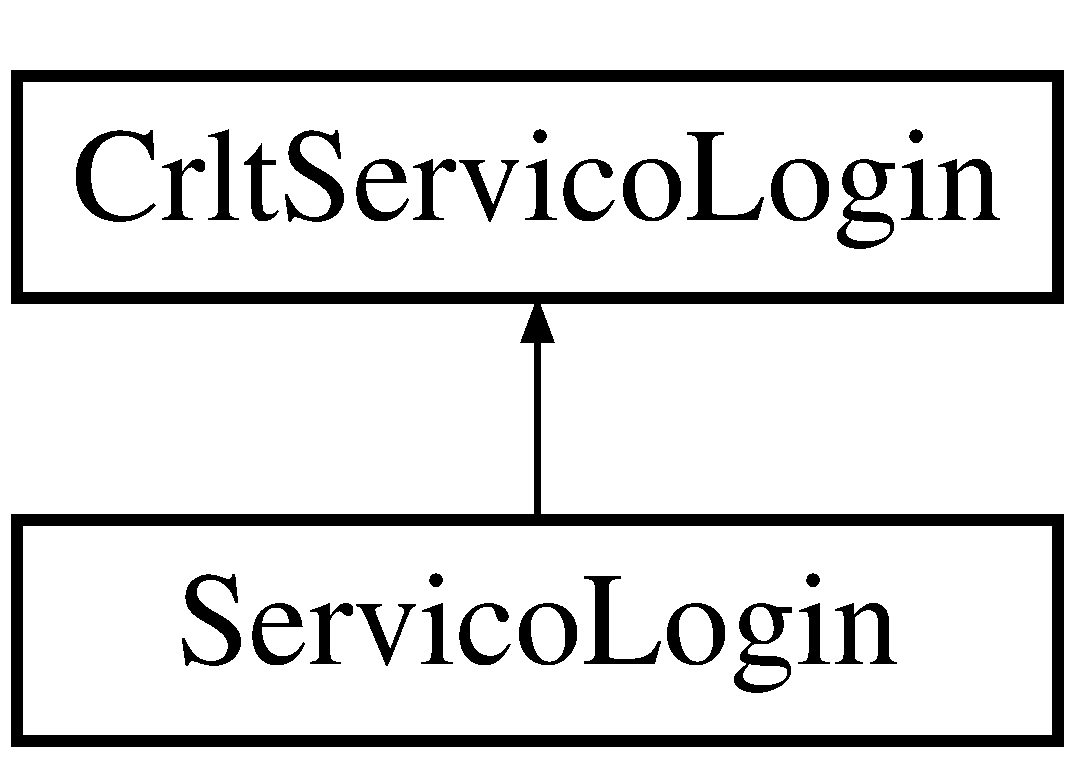
\includegraphics[height=2.000000cm]{class_servico_login}
\end{center}
\end{figure}
\subsection*{Membros Públicos}
\begin{DoxyCompactItemize}
\item 
string \mbox{\hyperlink{class_servico_login_a0dd44bd72da82fa932e4929edbefb6ea}{login}} (int opcao, string email, string senha)
\item 
void \mbox{\hyperlink{class_servico_login_ae6786007e98ac8288dc53d025d5f5bcd}{criar\+Usuario\+Leitor}} ()
\item 
void \mbox{\hyperlink{class_servico_login_aff5fc69ce9c3fa82c6c575f025ac2a34}{criar\+Usuario\+Desenvolvedor}} ()
\item 
void \mbox{\hyperlink{class_servico_login_a2f7e5d945f4ce6b06c8ce093ed3755e7}{criar\+Usuario\+Administrador}} ()
\end{DoxyCompactItemize}


\subsection{Funções membros}
\mbox{\Hypertarget{class_servico_login_a2f7e5d945f4ce6b06c8ce093ed3755e7}\label{class_servico_login_a2f7e5d945f4ce6b06c8ce093ed3755e7}} 
\index{Servico\+Login@{Servico\+Login}!criar\+Usuario\+Administrador@{criar\+Usuario\+Administrador}}
\index{criar\+Usuario\+Administrador@{criar\+Usuario\+Administrador}!Servico\+Login@{Servico\+Login}}
\subsubsection{\texorpdfstring{criar\+Usuario\+Administrador()}{criarUsuarioAdministrador()}}
{\footnotesize\ttfamily void Servico\+Login\+::criar\+Usuario\+Administrador (\begin{DoxyParamCaption}{ }\end{DoxyParamCaption})\hspace{0.3cm}{\ttfamily [virtual]}}



Implementa \mbox{\hyperlink{class_crlt_servico_login_a49825818fa1e6e24495d6cb9e4236907}{Crlt\+Servico\+Login}}.


\begin{DoxyCode}
1425 \{
1426   \mbox{\hyperlink{class_nome}{Nome}} *nome = \textcolor{keyword}{new} \mbox{\hyperlink{class_nome}{Nome}}();
1427   \mbox{\hyperlink{class_sobrenome}{Sobrenome}} *sobrenome = \textcolor{keyword}{new} \mbox{\hyperlink{class_sobrenome}{Sobrenome}}();
1428   \mbox{\hyperlink{class_telefone}{Telefone}} *telefone = \textcolor{keyword}{new} \mbox{\hyperlink{class_telefone}{Telefone}}();
1429   \mbox{\hyperlink{class_endereco}{Endereco}} *endereco = \textcolor{keyword}{new} \mbox{\hyperlink{class_endereco}{Endereco}}();
1430   \mbox{\hyperlink{class_data}{Data}} *data = \textcolor{keyword}{new} \mbox{\hyperlink{class_data}{Data}}();
1431   \mbox{\hyperlink{class_email}{Email}} *email = \textcolor{keyword}{new} \mbox{\hyperlink{class_email}{Email}}();
1432   \mbox{\hyperlink{class_senha}{Senha}} *senha = \textcolor{keyword}{new} \mbox{\hyperlink{class_senha}{Senha}}();
1433   \textcolor{keywordtype}{string} query;
1434   \textcolor{keywordtype}{string} entrada;
1435   \textcolor{keywordtype}{int} resultado;
1436 
1437   cin.ignore();
1438   \textcolor{keywordflow}{while}(\textcolor{keyword}{true})
1439   \{
1440     \textcolor{keywordflow}{try}
1441     \{
1442       cout << \textcolor{stringliteral}{"Nome: "};
1443       getline(cin, entrada);
1444       nome->\mbox{\hyperlink{class_nome_a83b9f56ec9f86f4b976846f4c5c65b30}{setNome}}(entrada);
1445 
1446       cout << \textcolor{stringliteral}{"Sobrenome: "};
1447       getline(cin, entrada);
1448       sobrenome->\mbox{\hyperlink{class_sobrenome_a9dc2277e3600656838e47c86dfddd23a}{setSobrenome}}(entrada);
1449 
1450       cout << \textcolor{stringliteral}{"Data de nascimento: "};
1451       getline(cin, entrada);
1452       data->\mbox{\hyperlink{class_data_a5245638838a033c98a8b760836dddb7d}{setData}}(entrada);
1453 
1454       cout << \textcolor{stringliteral}{"Telefone: "};
1455       getline(cin, entrada);
1456       telefone->\mbox{\hyperlink{class_telefone_ad85910fc35320e4a8e7ede8d40bbc454}{setTelefone}}(entrada);
1457 
1458       cout << \textcolor{stringliteral}{"Endereco: "};
1459       getline(cin, entrada);
1460       endereco->\mbox{\hyperlink{class_endereco_a36e8c19c5e97f321d77aece5b3e53239}{setEndereco}}(entrada);
1461 
1462       cout << \textcolor{stringliteral}{"Email: "};
1463       getline(cin, entrada);
1464       email->\mbox{\hyperlink{class_email_a2614b3a19d961411d1bece9c1bdf616f}{setEmail}}(entrada);
1465 
1466       cout << \textcolor{stringliteral}{"Senha: "};
1467       getline(cin, entrada);
1468       senha->\mbox{\hyperlink{class_senha_a01bbc2a82c5f405b68f33fe0dc538ec1}{setSenha}}(entrada,nome);
1469 
1470       \textcolor{keywordflow}{break};
1471 
1472     \}
1473     \textcolor{keywordflow}{catch}(\textcolor{keyword}{const} \textcolor{keywordtype}{char} *erro)
1474     \{
1475       cout << erro << endl;
1476     \}
1477   \}
1478 
1479   \mbox{\hyperlink{comando_sql_8cpp_a4f89ddcbc4cf8f2587d89f72f8c7900d}{conectarDbUsuario}}();
1480 
1481   query = \textcolor{stringliteral}{"insert into Administradores(nome,sobrenome,telefone,endereco,data,email,senha) "};
1482   query += \textcolor{stringliteral}{"values('"};
1483   query += nome->\mbox{\hyperlink{class_nome_aad41176173eec20cbbae1576447a3697}{getNome}}();
1484   query += \textcolor{stringliteral}{"','"};
1485   query += sobrenome->\mbox{\hyperlink{class_sobrenome_a954491366ce07f6715f32a97d67edf04}{getSobrenome}}();
1486   query += \textcolor{stringliteral}{"','"};
1487   query += telefone->\mbox{\hyperlink{class_telefone_a3e7acb7a3b658ef9e5d73b7e1d2948e7}{getTelefone}}();
1488   query += \textcolor{stringliteral}{"','"};
1489   query += endereco->\mbox{\hyperlink{class_endereco_aa1ccbda52f9559a68379c54e7e914d19}{getEndereco}}();
1490   query += \textcolor{stringliteral}{"','"};
1491   query += data->\mbox{\hyperlink{class_data_afc7b15a5e81334858e48709b2f45cdc3}{getData}}();
1492   query += \textcolor{stringliteral}{"','"};
1493   query += email->\mbox{\hyperlink{class_email_aa9a0e1a66b4efde65cf017bdd1c6c625}{getEmail}}();
1494   query += \textcolor{stringliteral}{"','"};
1495   query += senha->\mbox{\hyperlink{class_senha_a8786b3d03b1652e73df1cdce46cbbaaf}{getSenha}}();
1496   query += \textcolor{stringliteral}{"');"};
1497 
1498   resultado = \mbox{\hyperlink{comando_sql_8cpp_a748197580e7f9acdbf48c78de1f7924b}{executDbUsuario}}(query);
1499 
1500   query = \textcolor{stringliteral}{"select count(*) from Administradores where email = '"};
1501   query += email->\mbox{\hyperlink{class_email_aa9a0e1a66b4efde65cf017bdd1c6c625}{getEmail}}();
1502   query += \textcolor{stringliteral}{"' and senha = '"};
1503   query += senha->\mbox{\hyperlink{class_senha_a8786b3d03b1652e73df1cdce46cbbaaf}{getSenha}}();
1504   query += \textcolor{stringliteral}{"';"};
1505 
1506   resultado = \mbox{\hyperlink{comando_sql_8cpp_af54952694f2fa7d76f969fb74b853cb9}{executDbUsuarioRows}}(query);
1507 
1508   \textcolor{keywordflow}{if}(resultado != -1)
1509   \{
1510     \textcolor{keywordflow}{throw} \textcolor{stringliteral}{"\(\backslash\)t---------------- Cadastrado realizado com sucesso ----------------\(\backslash\)n"};
1511   \}
1512   \textcolor{keywordflow}{else}
1513   \{
1514     \textcolor{keywordflow}{throw} \textcolor{stringliteral}{"Erro na realizacao do cadastro...\(\backslash\)n\(\backslash\)n"};
1515   \}
1516 
1517 \mbox{\hyperlink{comando_sql_8cpp_a969be9911913568e30d4ae8963338bc3}{desconectarDbUsuario}}();
1518 
1519 \}
\end{DoxyCode}
\mbox{\Hypertarget{class_servico_login_aff5fc69ce9c3fa82c6c575f025ac2a34}\label{class_servico_login_aff5fc69ce9c3fa82c6c575f025ac2a34}} 
\index{Servico\+Login@{Servico\+Login}!criar\+Usuario\+Desenvolvedor@{criar\+Usuario\+Desenvolvedor}}
\index{criar\+Usuario\+Desenvolvedor@{criar\+Usuario\+Desenvolvedor}!Servico\+Login@{Servico\+Login}}
\subsubsection{\texorpdfstring{criar\+Usuario\+Desenvolvedor()}{criarUsuarioDesenvolvedor()}}
{\footnotesize\ttfamily void Servico\+Login\+::criar\+Usuario\+Desenvolvedor (\begin{DoxyParamCaption}{ }\end{DoxyParamCaption})\hspace{0.3cm}{\ttfamily [virtual]}}

Funcao responsavel pelo cadastramento de novos desenvolvedores no sistema. Primeiramente sao criados instancias de objetos no qual esses objetos irao compor o cadastro do desenvolvedor. Apos isso, e pedido para que o usuario digite as informacoes pedidas, e assim as mesmas passaram por um processo de validacao feito o processo de validacao, essas informacoes finalmente sera gravadas no DB de desenvolvedores, e apos essa gravacao uma query e executada em busca do novo membro, retornando assim o valor da pesquisa, chegando a conclusao se o desenvolvedor foi criado com sucesso ou nao.

Implementa \mbox{\hyperlink{class_crlt_servico_login_aab452ac1f3d0fd6d2f6989017026b188}{Crlt\+Servico\+Login}}.


\begin{DoxyCode}
539 \{
548     \mbox{\hyperlink{class_nome}{Nome}} *nome = \textcolor{keyword}{new} \mbox{\hyperlink{class_nome}{Nome}}();
549     \mbox{\hyperlink{class_sobrenome}{Sobrenome}} *sobrenome = \textcolor{keyword}{new} \mbox{\hyperlink{class_sobrenome}{Sobrenome}}();
550     \mbox{\hyperlink{class_data}{Data}} *data = \textcolor{keyword}{new} \mbox{\hyperlink{class_data}{Data}}();
551     \mbox{\hyperlink{class_email}{Email}} *email = \textcolor{keyword}{new} \mbox{\hyperlink{class_email}{Email}}();
552     \mbox{\hyperlink{class_senha}{Senha}} *senha = \textcolor{keyword}{new} \mbox{\hyperlink{class_senha}{Senha}}();
553     \mbox{\hyperlink{class_desenvolvedor}{Desenvolvedor}} *desenvolvedor = \textcolor{keyword}{new} \mbox{\hyperlink{class_desenvolvedor}{Desenvolvedor}}();
554     \textcolor{keywordtype}{string} entrada;
555     \textcolor{keywordtype}{string} query;
556     \textcolor{keywordtype}{int} resultado;
557     cin.ignore();
558     \textcolor{keywordflow}{while}(\textcolor{keyword}{true})
559     \{
560       \textcolor{keywordflow}{try}
561       \{
562         cout << \textcolor{stringliteral}{"Nome: "};
563         getline(cin, entrada);
564         nome->\mbox{\hyperlink{class_nome_a83b9f56ec9f86f4b976846f4c5c65b30}{setNome}}(entrada);
565 
566         cout << \textcolor{stringliteral}{"Sobrenome: "};
567         getline(cin, entrada);
568         sobrenome->\mbox{\hyperlink{class_sobrenome_a9dc2277e3600656838e47c86dfddd23a}{setSobrenome}}(entrada);
569 
570         cout << \textcolor{stringliteral}{"Data de Nascimento: "};
571         getline(cin, entrada);
572         data->\mbox{\hyperlink{class_data_a5245638838a033c98a8b760836dddb7d}{setData}}(entrada);
573 
574         cout << \textcolor{stringliteral}{"Email: "};
575         getline(cin, entrada);
576         email->\mbox{\hyperlink{class_email_a2614b3a19d961411d1bece9c1bdf616f}{setEmail}}(entrada);
577 
578         cout << \textcolor{stringliteral}{"Senha: "};
579         getline(cin, entrada);
580         senha->\mbox{\hyperlink{class_senha_a01bbc2a82c5f405b68f33fe0dc538ec1}{setSenha}}(entrada,nome);
581 
582         \textcolor{keywordflow}{break};
583 
584       \}
585       \textcolor{keywordflow}{catch}(\textcolor{keyword}{const} \textcolor{keywordtype}{char} *erro)
586       \{
587         cout << erro << endl;
588       \}
589     \}
590 
591     \mbox{\hyperlink{comando_sql_8cpp_a4f89ddcbc4cf8f2587d89f72f8c7900d}{conectarDbUsuario}}();
592 
593     query = \textcolor{stringliteral}{"insert into Desenvolvedores(nome,sobrenome,data,email,senha) "};
594     query += \textcolor{stringliteral}{"values('"};
595     query += nome->\mbox{\hyperlink{class_nome_aad41176173eec20cbbae1576447a3697}{getNome}}();
596     query += \textcolor{stringliteral}{"','"};
597     query += sobrenome->\mbox{\hyperlink{class_sobrenome_a954491366ce07f6715f32a97d67edf04}{getSobrenome}}();
598     query += \textcolor{stringliteral}{"','"};
599     query += data->\mbox{\hyperlink{class_data_afc7b15a5e81334858e48709b2f45cdc3}{getData}}();
600     query += \textcolor{stringliteral}{"','"};
601     query += email->\mbox{\hyperlink{class_email_aa9a0e1a66b4efde65cf017bdd1c6c625}{getEmail}}();
602     query += \textcolor{stringliteral}{"','"};
603     query += senha->\mbox{\hyperlink{class_senha_a8786b3d03b1652e73df1cdce46cbbaaf}{getSenha}}();
604     query += \textcolor{stringliteral}{"');"};
605 
606 
607     resultado = \mbox{\hyperlink{comando_sql_8cpp_a748197580e7f9acdbf48c78de1f7924b}{executDbUsuario}}(query);
608 
609     query = \textcolor{stringliteral}{"select count(*) from Desenvolvedores where email = '"};
610     query += email->\mbox{\hyperlink{class_email_aa9a0e1a66b4efde65cf017bdd1c6c625}{getEmail}}();
611     query += \textcolor{stringliteral}{"' and senha = '"};
612     query += senha->\mbox{\hyperlink{class_senha_a8786b3d03b1652e73df1cdce46cbbaaf}{getSenha}}();
613     query += \textcolor{stringliteral}{"';"};
614 
615     resultado = \mbox{\hyperlink{comando_sql_8cpp_af54952694f2fa7d76f969fb74b853cb9}{executDbUsuarioRows}}(query);
616 
617     \textcolor{keywordflow}{if}(resultado != -1)
618     \{
619       \textcolor{keywordflow}{throw} \textcolor{stringliteral}{"\(\backslash\)t------------ Usuario desenvolvedor criado com sucesso ------------\(\backslash\)n"};
620     \}
621     \textcolor{keywordflow}{else}
622     \{
623       \textcolor{keywordflow}{throw} \textcolor{stringliteral}{"Erro ao criar usuario...\(\backslash\)n\(\backslash\)n"};
624     \}
625 
626     \mbox{\hyperlink{comando_sql_8cpp_a969be9911913568e30d4ae8963338bc3}{desconectarDbUsuario}}();
627 
628 \}
\end{DoxyCode}
\mbox{\Hypertarget{class_servico_login_ae6786007e98ac8288dc53d025d5f5bcd}\label{class_servico_login_ae6786007e98ac8288dc53d025d5f5bcd}} 
\index{Servico\+Login@{Servico\+Login}!criar\+Usuario\+Leitor@{criar\+Usuario\+Leitor}}
\index{criar\+Usuario\+Leitor@{criar\+Usuario\+Leitor}!Servico\+Login@{Servico\+Login}}
\subsubsection{\texorpdfstring{criar\+Usuario\+Leitor()}{criarUsuarioLeitor()}}
{\footnotesize\ttfamily void Servico\+Login\+::criar\+Usuario\+Leitor (\begin{DoxyParamCaption}{ }\end{DoxyParamCaption})\hspace{0.3cm}{\ttfamily [virtual]}}

Funcao para criar um novo usuario do tipo leitor. Primeiramente sao criados objetos que fazem parte das informacoes que um leitor precisa disponibilizar para poder se cadastrar no sistema, que sao eles\+: nome,sobrenome,email, senha. Cada uma dessas informacoes sera testada e aprovada pelo sistema antes de serem jogadas dentro do banco de Dados Feita a conexao com o DB, as informacoes sao pedidas e as validacoes devidamente realizadas Feito isso uma query e montada para jogar as informacoes na tabela correspondente tipo de Cadastro que foi realizado, nesse caso, do tipo leitor. Apos isso uma nova query e criada pesquisando pelo email criado e se retornar 1, significa que o usuario foi criado com sucesso.

Implementa \mbox{\hyperlink{class_crlt_servico_login_ab5fdf7e56eb8edd6113386011f161085}{Crlt\+Servico\+Login}}.


\begin{DoxyCode}
138 \{
149   \mbox{\hyperlink{class_nome}{Nome}} *nome = \textcolor{keyword}{new} \mbox{\hyperlink{class_nome}{Nome}}();
150   \mbox{\hyperlink{class_sobrenome}{Sobrenome}} *sobrenome = \textcolor{keyword}{new} \mbox{\hyperlink{class_sobrenome}{Sobrenome}}();
151   \mbox{\hyperlink{class_email}{Email}} *email = \textcolor{keyword}{new} \mbox{\hyperlink{class_email}{Email}}();
152   \mbox{\hyperlink{class_senha}{Senha}} *senha = \textcolor{keyword}{new} \mbox{\hyperlink{class_senha}{Senha}}();
153   \textcolor{keywordtype}{int} consulta,recebe;
154   \textcolor{keywordtype}{string} query;
155   \textcolor{keywordtype}{int} resultado;
156   \textcolor{keywordtype}{string} entrada;
157 
158   \mbox{\hyperlink{comando_sql_8cpp_a4f89ddcbc4cf8f2587d89f72f8c7900d}{conectarDbUsuario}}();
159   cin.ignore();
160   \textcolor{keywordflow}{while}(\textcolor{keyword}{true})
161   \{
162     \textcolor{keywordflow}{try}
163     \{
164       cout << \textcolor{stringliteral}{"Nome: "};
165       getline(cin, entrada);
166       nome->\mbox{\hyperlink{class_nome_a83b9f56ec9f86f4b976846f4c5c65b30}{setNome}}(entrada);
167 
168       cout << \textcolor{stringliteral}{"Sobrenome: "};
169       getline(cin, entrada);
170       sobrenome->\mbox{\hyperlink{class_sobrenome_a9dc2277e3600656838e47c86dfddd23a}{setSobrenome}}(entrada);
171 
172       cout << \textcolor{stringliteral}{"Email: "};
173       getline(cin, entrada);
174       email->\mbox{\hyperlink{class_email_a2614b3a19d961411d1bece9c1bdf616f}{setEmail}}(entrada);
175       query = \textcolor{stringliteral}{"select count(*) from Leitores where email = '"};
176       query += email->\mbox{\hyperlink{class_email_aa9a0e1a66b4efde65cf017bdd1c6c625}{getEmail}}();
177       query += \textcolor{stringliteral}{"';"};
178       resultado = \mbox{\hyperlink{comando_sql_8cpp_af54952694f2fa7d76f969fb74b853cb9}{executDbUsuarioRows}}(query);
179       \textcolor{keywordflow}{if}(resultado != -1)
180       \{
181         \textcolor{keywordflow}{throw} \textcolor{stringliteral}{"Erro, email ja possui cadastro\(\backslash\)n\(\backslash\)n"};
182       \}
183 
184       cout << \textcolor{stringliteral}{"Senha: "};
185       getline(cin, entrada);
186       senha->\mbox{\hyperlink{class_senha_a01bbc2a82c5f405b68f33fe0dc538ec1}{setSenha}}(entrada,nome);
187 
188       \textcolor{keywordflow}{break};
189 
190     \}
191     \textcolor{keywordflow}{catch}(\textcolor{keyword}{const} \textcolor{keywordtype}{char} *erro)
192     \{
193       cout << erro << endl;
194     \}
195   \}
196 
197   query = \textcolor{stringliteral}{"INSERT INTO Leitores (nome,sobrenome,email,senha) "};
198   query += \textcolor{stringliteral}{"VALUES ('"};
199   query += nome->\mbox{\hyperlink{class_nome_aad41176173eec20cbbae1576447a3697}{getNome}}();
200   query += \textcolor{stringliteral}{"','"};
201   query += sobrenome->\mbox{\hyperlink{class_sobrenome_a954491366ce07f6715f32a97d67edf04}{getSobrenome}}();
202   query += \textcolor{stringliteral}{"','"};
203   query += email->\mbox{\hyperlink{class_email_aa9a0e1a66b4efde65cf017bdd1c6c625}{getEmail}}();
204   query += \textcolor{stringliteral}{"','"};
205   query += senha->\mbox{\hyperlink{class_senha_a8786b3d03b1652e73df1cdce46cbbaaf}{getSenha}}();
206   query += \textcolor{stringliteral}{"');"};
207 
208   recebe = \mbox{\hyperlink{comando_sql_8cpp_a748197580e7f9acdbf48c78de1f7924b}{executDbUsuario}}(query);
209 
210   query = \textcolor{stringliteral}{"select count(*) from Leitores where email = '"};
211   query += email->\mbox{\hyperlink{class_email_aa9a0e1a66b4efde65cf017bdd1c6c625}{getEmail}}();
212   query += \textcolor{stringliteral}{"';"};
213 
214   resultado = \mbox{\hyperlink{comando_sql_8cpp_af54952694f2fa7d76f969fb74b853cb9}{executDbUsuarioRows}}(query);
215 
216   \textcolor{keywordflow}{if}(resultado == -1)
217   \{
218     \textcolor{keywordflow}{throw} \textcolor{stringliteral}{"Erro ao criar usuario....\(\backslash\)n\(\backslash\)n"};
219   \}
220   \textcolor{keywordflow}{else}
221   \{
222     \textcolor{keywordflow}{throw} \textcolor{stringliteral}{"\(\backslash\)t------------ Usuario Leitor criado com sucesso ------------\(\backslash\)n"};
223   \}
224 
225   \mbox{\hyperlink{comando_sql_8cpp_a969be9911913568e30d4ae8963338bc3}{desconectarDbUsuario}}();
226 
227 \}
\end{DoxyCode}
\mbox{\Hypertarget{class_servico_login_a0dd44bd72da82fa932e4929edbefb6ea}\label{class_servico_login_a0dd44bd72da82fa932e4929edbefb6ea}} 
\index{Servico\+Login@{Servico\+Login}!login@{login}}
\index{login@{login}!Servico\+Login@{Servico\+Login}}
\subsubsection{\texorpdfstring{login()}{login()}}
{\footnotesize\ttfamily string Servico\+Login\+::login (\begin{DoxyParamCaption}\item[{int}]{opcao,  }\item[{string}]{email,  }\item[{string}]{senha }\end{DoxyParamCaption})\hspace{0.3cm}{\ttfamily [virtual]}}

Implementacao da funcao login na qual recebe dois parametros, o primeiro e a opcao feita pelo usuario, podendo ser os numeros de um ate o quatro, cada um com sua respectiva funcao, os outros dois parametros sao o e-\/mail e senha que sao utilizados quando o usuario loga como leitor, desenvolvedor ou administrador, porem quando o usuario quer criar uma conta, esses parametros sao meramente ilustrativos

Implementa \mbox{\hyperlink{class_crlt_servico_login_a3a863ed6ef16279d0cdc1d33fd8f5edd}{Crlt\+Servico\+Login}}.


\begin{DoxyCode}
4 \{
12   \textcolor{keywordtype}{int} resultado;
13   \textcolor{keywordtype}{string} query;
14   \textcolor{keywordtype}{int} escolhaConta;
15   \mbox{\hyperlink{comando_sql_8cpp_a4f89ddcbc4cf8f2587d89f72f8c7900d}{conectarDbUsuario}}();
16 
17   \textcolor{keywordflow}{if}(opcao == 1)
18   \{
19     query = \textcolor{stringliteral}{"select count(*) from Leitores where email='"};
20     query += email;
21     query += \textcolor{stringliteral}{"' and senha ='"};
22     query += senha;
23     query += \textcolor{stringliteral}{"';"};
24     resultado = \mbox{\hyperlink{comando_sql_8cpp_af54952694f2fa7d76f969fb74b853cb9}{executDbUsuarioRows}}(query);
25 
26     \textcolor{keywordflow}{if}(resultado != -1)
27     \{
28       \mbox{\hyperlink{comando_sql_8cpp_a969be9911913568e30d4ae8963338bc3}{desconectarDbUsuario}}();
29       \textcolor{keywordflow}{return} \textcolor{stringliteral}{"leitor"};
30     \}
31   \}
32 
33   \textcolor{keywordflow}{if}(opcao == 2)
34   \{
35     query = \textcolor{stringliteral}{"select count(*) from Desenvolvedores where email='"};
36     query += email;
37     query += \textcolor{stringliteral}{"' and senha ='"};
38     query += senha;
39     query += \textcolor{stringliteral}{"';"};
40     resultado = \mbox{\hyperlink{comando_sql_8cpp_af54952694f2fa7d76f969fb74b853cb9}{executDbUsuarioRows}}(query);
41 
42     \textcolor{keywordflow}{if}(resultado != -1)
43     \{
44       \mbox{\hyperlink{comando_sql_8cpp_a969be9911913568e30d4ae8963338bc3}{desconectarDbUsuario}}();
45       \textcolor{keywordflow}{return} \textcolor{stringliteral}{"desenvolvedor"};
46     \}
47   \}
48 
49   \textcolor{keywordflow}{if}(opcao == 3)
50   \{
51     query = \textcolor{stringliteral}{"select count(*) from Administradores where email='"};
52     query += email;
53     query += \textcolor{stringliteral}{"' and senha ='"};
54     query += senha;
55     query += \textcolor{stringliteral}{"';"};
56     resultado = \mbox{\hyperlink{comando_sql_8cpp_af54952694f2fa7d76f969fb74b853cb9}{executDbUsuarioRows}}(query);
57 
58     \textcolor{keywordflow}{if}(resultado != -1)
59     \{
60       \mbox{\hyperlink{comando_sql_8cpp_a969be9911913568e30d4ae8963338bc3}{desconectarDbUsuario}}();
61       \textcolor{keywordflow}{return} \textcolor{stringliteral}{"administrador"};
62     \}
63   \}
64 
65   \textcolor{keywordflow}{if}(opcao == 4)
66   \{
67     \textcolor{keywordflow}{while}(\textcolor{keyword}{true})
68     \{
69       cout << \textcolor{stringliteral}{"1 - Criar conta leitor\(\backslash\)n"};
70       cout << \textcolor{stringliteral}{"2 - Criar conta Desenvolvedor\(\backslash\)n"};
71       cout << \textcolor{stringliteral}{"3 - Criar conta Administrador\(\backslash\)n\(\backslash\)n"};
72       cout << \textcolor{stringliteral}{"Selecione a opcao desejada: "};
73       cin >> escolhaConta;
74 
75       \textcolor{keywordflow}{if}(escolhaConta == 1)
76       \{
77         \mbox{\hyperlink{class_servico_login_ae6786007e98ac8288dc53d025d5f5bcd}{criarUsuarioLeitor}}();
78         \textcolor{keywordflow}{break};
79       \}
80       \textcolor{keywordflow}{else}
81       \{
82         \textcolor{keywordflow}{if}(escolhaConta == 2)
83         \{
84           \mbox{\hyperlink{class_servico_login_aff5fc69ce9c3fa82c6c575f025ac2a34}{criarUsuarioDesenvolvedor}}();
85           \textcolor{keywordflow}{break};
86         \}
87         \textcolor{keywordflow}{else}
88         \{
89           \textcolor{keywordflow}{if}(escolhaConta == 3)
90           \{
91             \mbox{\hyperlink{class_servico_login_a2f7e5d945f4ce6b06c8ce093ed3755e7}{criarUsuarioAdministrador}}();
92             \textcolor{keywordflow}{break};
93           \}
94           \textcolor{keywordflow}{else}
95           \{
96             cout << \textcolor{stringliteral}{"Opcao invalida, tente novamente...\(\backslash\)n\(\backslash\)n"};
97           \}
98         \}
99       \}
100     \}
101   \}
102 
103   \mbox{\hyperlink{comando_sql_8cpp_a969be9911913568e30d4ae8963338bc3}{desconectarDbUsuario}}();
104   \textcolor{keywordflow}{return} \textcolor{stringliteral}{"erro"};
105 \}
\end{DoxyCode}


A documentação para essa classe foi gerada a partir dos seguintes arquivos\+:\begin{DoxyCompactItemize}
\item 
/\+Users/amadeulinhares/\+Desktop/\+Trabalho3/\mbox{\hyperlink{servico_8hpp}{servico.\+hpp}}\item 
/\+Users/amadeulinhares/\+Desktop/\+Trabalho3/\mbox{\hyperlink{servico_8cpp}{servico.\+cpp}}\end{DoxyCompactItemize}

\hypertarget{class_servico_usuarios_administrador}{}\section{Referência da Classe Servico\+Usuarios\+Administrador}
\label{class_servico_usuarios_administrador}\index{Servico\+Usuarios\+Administrador@{Servico\+Usuarios\+Administrador}}


{\ttfamily \#include $<$servico.\+hpp$>$}

Diagrama de hierarquia para Servico\+Usuarios\+Administrador\+:\begin{figure}[H]
\begin{center}
\leavevmode
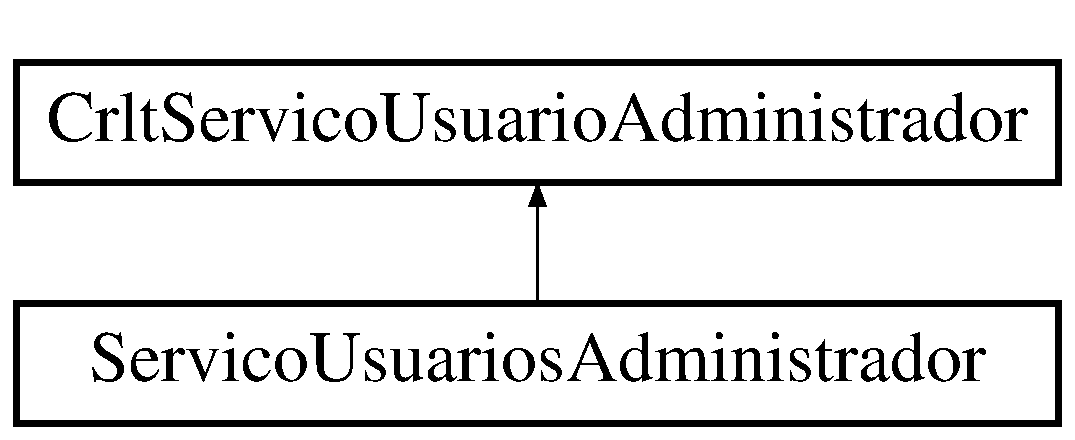
\includegraphics[height=2.000000cm]{class_servico_usuarios_administrador}
\end{center}
\end{figure}
\subsection*{Membros Públicos}
\begin{DoxyCompactItemize}
\item 
void \mbox{\hyperlink{class_servico_usuarios_administrador_ae1474bec1c712ba5640c83f4fe666fc4}{consultar\+Cadastro\+Administrador}} (string email)
\item 
void \mbox{\hyperlink{class_servico_usuarios_administrador_a1295e808f5e6322a8e329ff711b2b428}{excluir\+Usuario\+Administrador}} (string email)
\item 
void \mbox{\hyperlink{class_servico_usuarios_administrador_a1111b56d40dff5aa7186c4f3dfe2e598}{atualizar\+Usuario\+Administrador}} (string email)
\item 
void \mbox{\hyperlink{class_servico_usuarios_administrador_a72b7761474e413704531b3234744d0e0}{list\+Nome\+Vocabularios}} ()
\item 
void \mbox{\hyperlink{class_servico_usuarios_administrador_adddc69a01b3ffb101f3a0b5825dde223}{list\+Dados\+Vocabulario}} ()
\item 
void \mbox{\hyperlink{class_servico_usuarios_administrador_aec8b05b7c4a2fb318b6be8f6704d68eb}{consultar\+Termo}} ()
\item 
void \mbox{\hyperlink{class_servico_usuarios_administrador_acc178ea9b5ed289bde27ca853e874962}{consultar\+Definicao\+Termo}} ()
\item 
void \mbox{\hyperlink{class_servico_usuarios_administrador_a0a20923a2c556fa62587fac48b6e55da}{cadastra\+Desenvolvedor\+Voc\+Controlado}} (string email)
\item 
void \mbox{\hyperlink{class_servico_usuarios_administrador_a9002054e8a06338e2a380517b6aeb1f7}{cria\+Termo}} ()
\item 
void \mbox{\hyperlink{class_servico_usuarios_administrador_a219b135060f3a85d996f506474b99f48}{editar\+Termo}} ()
\item 
void \mbox{\hyperlink{class_servico_usuarios_administrador_a90abacb7bb051878e6b016d9993733c1}{excluir\+Termo}} ()
\item 
void \mbox{\hyperlink{class_servico_usuarios_administrador_a10298cc0f8e8c1b6f44363747bc8de1e}{cria\+Definicao}} ()
\item 
void \mbox{\hyperlink{class_servico_usuarios_administrador_a1c78a37ca8e92725926d3f13299a50b6}{excluir\+Definicao}} ()
\item 
void \mbox{\hyperlink{class_servico_usuarios_administrador_aa1bda96596ffda5676af7181eaae9466}{editar\+Definicao}} ()
\item 
void \mbox{\hyperlink{class_servico_usuarios_administrador_abf155b3f2f19bf2ab2e3329a1587c750}{opcao\+Escolhida\+Administrador}} (int opcao, string email)
\item 
void \mbox{\hyperlink{class_servico_usuarios_administrador_a87f2dca2e2b3858f663b4220f357d26f}{criar\+Vocabulario}} (string email)
\item 
void \mbox{\hyperlink{class_servico_usuarios_administrador_a57d5f777ed99a006dc2db5cdb0f135b1}{editar\+Def\+Vocabulario}} ()
\item 
void \mbox{\hyperlink{class_servico_usuarios_administrador_ac0d400904b25cd30911a446bce66603a}{editar\+Idioma\+Voc}} ()
\item 
void \mbox{\hyperlink{class_servico_usuarios_administrador_a13237b760df88f3f8a825a5bcd1d7331}{excluir\+Vocabulario}} ()
\end{DoxyCompactItemize}


\subsection{Funções membros}
\mbox{\Hypertarget{class_servico_usuarios_administrador_a1111b56d40dff5aa7186c4f3dfe2e598}\label{class_servico_usuarios_administrador_a1111b56d40dff5aa7186c4f3dfe2e598}} 
\index{Servico\+Usuarios\+Administrador@{Servico\+Usuarios\+Administrador}!atualizar\+Usuario\+Administrador@{atualizar\+Usuario\+Administrador}}
\index{atualizar\+Usuario\+Administrador@{atualizar\+Usuario\+Administrador}!Servico\+Usuarios\+Administrador@{Servico\+Usuarios\+Administrador}}
\subsubsection{\texorpdfstring{atualizar\+Usuario\+Administrador()}{atualizarUsuarioAdministrador()}}
{\footnotesize\ttfamily void Servico\+Usuarios\+Administrador\+::atualizar\+Usuario\+Administrador (\begin{DoxyParamCaption}\item[{string}]{email }\end{DoxyParamCaption})\hspace{0.3cm}{\ttfamily [virtual]}}



Implementa \mbox{\hyperlink{class_crlt_servico_usuario_administrador_ab0492870331c189997ea174f0482202e}{Crlt\+Servico\+Usuario\+Administrador}}.


\begin{DoxyCode}
1784 \{
1785   \mbox{\hyperlink{class_nome}{Nome}} *nome = \textcolor{keyword}{new} \mbox{\hyperlink{class_nome}{Nome}}();
1786   \mbox{\hyperlink{class_sobrenome}{Sobrenome}} *sobrenome = \textcolor{keyword}{new} \mbox{\hyperlink{class_sobrenome}{Sobrenome}}();
1787   \mbox{\hyperlink{class_telefone}{Telefone}} *telefone = \textcolor{keyword}{new} \mbox{\hyperlink{class_telefone}{Telefone}}();
1788   \mbox{\hyperlink{class_endereco}{Endereco}} *endereco = \textcolor{keyword}{new} \mbox{\hyperlink{class_endereco}{Endereco}}();
1789   \mbox{\hyperlink{class_data}{Data}} *data = \textcolor{keyword}{new} \mbox{\hyperlink{class_data}{Data}}();
1790   \mbox{\hyperlink{class_email}{Email}} *emailAtualiza = \textcolor{keyword}{new} \mbox{\hyperlink{class_email}{Email}}();
1791   \mbox{\hyperlink{class_senha}{Senha}} *senha = \textcolor{keyword}{new} \mbox{\hyperlink{class_senha}{Senha}}();
1792   \textcolor{keywordtype}{string} query;
1793   \textcolor{keywordtype}{string} entrada;
1794   \textcolor{keywordtype}{int} resultado;
1795 
1796   cin.ignore();
1797   \textcolor{keywordflow}{while}(\textcolor{keyword}{true})
1798   \{
1799     \textcolor{keywordflow}{try}
1800     \{
1801       cout << \textcolor{stringliteral}{"Nome: "};
1802       cin >> entrada;
1803       nome->\mbox{\hyperlink{class_nome_a83b9f56ec9f86f4b976846f4c5c65b30}{setNome}}(entrada);
1804 
1805       cout << \textcolor{stringliteral}{"Sobrenome: "};
1806       cin >> entrada;
1807       sobrenome->\mbox{\hyperlink{class_sobrenome_a9dc2277e3600656838e47c86dfddd23a}{setSobrenome}}(entrada);
1808 
1809       cout << \textcolor{stringliteral}{"Data de nascimento: "};
1810       cin >> entrada;
1811       data->\mbox{\hyperlink{class_data_a5245638838a033c98a8b760836dddb7d}{setData}}(entrada);
1812 
1813       cout << \textcolor{stringliteral}{"Telefone: "};
1814       cin >> entrada;
1815       telefone->\mbox{\hyperlink{class_telefone_ad85910fc35320e4a8e7ede8d40bbc454}{setTelefone}}(entrada);
1816       cin.ignore();
1817 
1818       cout << \textcolor{stringliteral}{"Endereco: "};
1819       getline(cin, entrada);
1820       endereco->\mbox{\hyperlink{class_endereco_a36e8c19c5e97f321d77aece5b3e53239}{setEndereco}}(entrada);
1821 
1822       cout << \textcolor{stringliteral}{"Email: "};
1823       cin >> entrada;
1824       emailAtualiza->\mbox{\hyperlink{class_email_a2614b3a19d961411d1bece9c1bdf616f}{setEmail}}(entrada);
1825       cin.ignore();
1826 
1827       cout << \textcolor{stringliteral}{"Senha: "};
1828       getline(cin, entrada);
1829       senha->\mbox{\hyperlink{class_senha_a01bbc2a82c5f405b68f33fe0dc538ec1}{setSenha}}(entrada,nome);
1830 
1831       \textcolor{keywordflow}{break};
1832 
1833     \}
1834     \textcolor{keywordflow}{catch}(\textcolor{keyword}{const} \textcolor{keywordtype}{char} *erro)
1835     \{
1836       cout << erro << endl;
1837     \}
1838   \}
1839 
1840   \mbox{\hyperlink{comando_sql_8cpp_a4f89ddcbc4cf8f2587d89f72f8c7900d}{conectarDbUsuario}}();
1841 
1842 
1843   query = \textcolor{stringliteral}{"update Administradores "};
1844   query += \textcolor{stringliteral}{"set nome = '"};
1845   query += nome->\mbox{\hyperlink{class_nome_aad41176173eec20cbbae1576447a3697}{getNome}}();
1846   query += \textcolor{stringliteral}{"', sobrenome = '"};
1847   query += sobrenome->\mbox{\hyperlink{class_sobrenome_a954491366ce07f6715f32a97d67edf04}{getSobrenome}}();
1848   query += \textcolor{stringliteral}{"', telefone = '"};
1849   query += telefone->\mbox{\hyperlink{class_telefone_a3e7acb7a3b658ef9e5d73b7e1d2948e7}{getTelefone}}();
1850   query += \textcolor{stringliteral}{"', endereco = '"};
1851   query += endereco->\mbox{\hyperlink{class_endereco_aa1ccbda52f9559a68379c54e7e914d19}{getEndereco}}();
1852   query += \textcolor{stringliteral}{"', data = '"};
1853   query += data->\mbox{\hyperlink{class_data_afc7b15a5e81334858e48709b2f45cdc3}{getData}}();
1854   query += \textcolor{stringliteral}{"', email = '"};
1855   query += emailAtualiza->\mbox{\hyperlink{class_email_aa9a0e1a66b4efde65cf017bdd1c6c625}{getEmail}}();
1856   query += \textcolor{stringliteral}{"', senha = '"};
1857   query += senha->\mbox{\hyperlink{class_senha_a8786b3d03b1652e73df1cdce46cbbaaf}{getSenha}}();
1858   query += \textcolor{stringliteral}{"' where email = '"};
1859   query += email;
1860   query += \textcolor{stringliteral}{"';"};
1861 
1862 
1863   resultado = \mbox{\hyperlink{comando_sql_8cpp_a748197580e7f9acdbf48c78de1f7924b}{executDbUsuario}}(query);
1864 
1865   query = \textcolor{stringliteral}{"select count(*) from Administradores where email = '"};
1866   query += emailAtualiza->\mbox{\hyperlink{class_email_aa9a0e1a66b4efde65cf017bdd1c6c625}{getEmail}}();
1867   query += \textcolor{stringliteral}{"';"};
1868 
1869   resultado = \mbox{\hyperlink{comando_sql_8cpp_af54952694f2fa7d76f969fb74b853cb9}{executDbUsuarioRows}}(query);
1870 
1871   \textcolor{keywordflow}{if}(resultado != -1)
1872   \{
1873     cout << \textcolor{stringliteral}{"\(\backslash\)t ---------------- Cadastro atualizado com sucesso ----------------\(\backslash\)n\(\backslash\)n"};
1874   \}
1875   \textcolor{keywordflow}{else}
1876   \{
1877     \textcolor{keywordflow}{throw} \textcolor{stringliteral}{"Erro ao atualizar cadastro...\(\backslash\)n\(\backslash\)n"};
1878   \}
1879 
1880 
1881 
1882 \}
\end{DoxyCode}
\mbox{\Hypertarget{class_servico_usuarios_administrador_a0a20923a2c556fa62587fac48b6e55da}\label{class_servico_usuarios_administrador_a0a20923a2c556fa62587fac48b6e55da}} 
\index{Servico\+Usuarios\+Administrador@{Servico\+Usuarios\+Administrador}!cadastra\+Desenvolvedor\+Voc\+Controlado@{cadastra\+Desenvolvedor\+Voc\+Controlado}}
\index{cadastra\+Desenvolvedor\+Voc\+Controlado@{cadastra\+Desenvolvedor\+Voc\+Controlado}!Servico\+Usuarios\+Administrador@{Servico\+Usuarios\+Administrador}}
\subsubsection{\texorpdfstring{cadastra\+Desenvolvedor\+Voc\+Controlado()}{cadastraDesenvolvedorVocControlado()}}
{\footnotesize\ttfamily void Servico\+Usuarios\+Administrador\+::cadastra\+Desenvolvedor\+Voc\+Controlado (\begin{DoxyParamCaption}\item[{string}]{email }\end{DoxyParamCaption})\hspace{0.3cm}{\ttfamily [virtual]}}



Implementa \mbox{\hyperlink{class_crlt_servico_usuario_administrador_ac0432bf5b0788a20f018781bcca74e45}{Crlt\+Servico\+Usuario\+Administrador}}.


\begin{DoxyCode}
2006 \{
2007   \textcolor{keywordtype}{string} vocabulario;
2008   \textcolor{keywordtype}{string} query;
2009   \textcolor{keywordtype}{int} resultado;
2010 
2011       cout << \textcolor{stringliteral}{"Digite o nome do vocabulario controlado no qual deseja se cadastrar: "};
2012       cin >> vocabulario;
2013 
2014       query = \textcolor{stringliteral}{"select count(*) from Vocabulario\_Controlado where nomeVocabulario = '"};
2015       query += vocabulario;
2016       query += \textcolor{stringliteral}{"';"};
2017 
2018 
2019       \mbox{\hyperlink{comando_sql_8cpp_a4f89ddcbc4cf8f2587d89f72f8c7900d}{conectarDbUsuario}}();
2020       resultado = \mbox{\hyperlink{comando_sql_8cpp_af54952694f2fa7d76f969fb74b853cb9}{executDbUsuarioRows}}(query);
2021 
2022       \textcolor{keywordflow}{if}(resultado == -1)
2023       \{
2024         \textcolor{keywordflow}{throw} \textcolor{stringliteral}{"Erro, Vocabulario Controlado nao encontrado\(\backslash\)n"};
2025       \}
2026 
2027         query = \textcolor{stringliteral}{"select count(*) from Vocabulario\_Controlado where desenvolvedores = '"};
2028         query += email;
2029         query += \textcolor{stringliteral}{"';"};
2030         resultado = \mbox{\hyperlink{comando_sql_8cpp_af54952694f2fa7d76f969fb74b853cb9}{executDbUsuarioRows}}(query);
2031 
2032         \textcolor{keywordflow}{if}(resultado != -1)
2033         \{
2034           \textcolor{keywordflow}{throw} \textcolor{stringliteral}{"Usuario ja possui cadastrado\(\backslash\)n"};
2035         \}
2036 
2037 
2038         query = \textcolor{stringliteral}{"select count(*) from Vocabulario\_Controlado where nome nomeVocabulario = '"};
2039         query += vocabulario;
2040         query += \textcolor{stringliteral}{"';"};
2041 
2042         resultado = \mbox{\hyperlink{comando_sql_8cpp_af54952694f2fa7d76f969fb74b853cb9}{executDbUsuarioRows}}(query);
2043 
2044         \textcolor{keywordflow}{if}(resultado >= 10)
2045         \{
2046           \textcolor{keywordflow}{throw} \textcolor{stringliteral}{"Numero de desenvolvedores esgotado para esse Vocabulario;\(\backslash\)n"};
2047         \}
2048 
2049 
2050 
2051         query = \textcolor{stringliteral}{"insert into Vocabulario\_Controlado (nomeVocabulario, idioma, emailAdmin)"};
2052         query += \textcolor{stringliteral}{"select nomeVocabulario, idioma, emailAdmin from Vocabulario\_Controlado where
       nomeVocabulario = '"};
2053         query += vocabulario;
2054         query += \textcolor{stringliteral}{"' and desenvolvedores = '-';"};
2055 
2056         resultado = \mbox{\hyperlink{comando_sql_8cpp_a748197580e7f9acdbf48c78de1f7924b}{executDbUsuario}}(query);
2057 
2058         query = \textcolor{stringliteral}{"update Vocabulario\_Controlado set desenvolvedores = '"};
2059         query += email;
2060         query += \textcolor{stringliteral}{"' where desenvolvedores is null and nomeVocabulario = '"};
2061         query += vocabulario;
2062         query += \textcolor{stringliteral}{"';"};
2063 
2064         resultado = \mbox{\hyperlink{comando_sql_8cpp_a748197580e7f9acdbf48c78de1f7924b}{executDbUsuario}}(query);
2065 
2066         cout << \textcolor{stringliteral}{"Processando comandos....\(\backslash\)n\(\backslash\)n"};
2067 
2068         query = \textcolor{stringliteral}{"select count(*) from Vocabulario\_Controlado where desenvolvedores = '"};
2069         query += email;
2070         query += \textcolor{stringliteral}{"';"};
2071 
2072           resultado = \mbox{\hyperlink{comando_sql_8cpp_af54952694f2fa7d76f969fb74b853cb9}{executDbUsuarioRows}}(query);
2073 
2074           \textcolor{keywordflow}{if}(resultado != -1)
2075           \{
2076             cout << \textcolor{stringliteral}{"Desenvolvedor adicionado com sucesso....\(\backslash\)n\(\backslash\)n"};
2077           \}
2078           \textcolor{keywordflow}{else}
2079           \{
2080             \textcolor{keywordflow}{throw} \textcolor{stringliteral}{"Erro na execução do comando\(\backslash\)n\(\backslash\)n"};
2081           \}
2082 
2083 \}
\end{DoxyCode}
\mbox{\Hypertarget{class_servico_usuarios_administrador_ae1474bec1c712ba5640c83f4fe666fc4}\label{class_servico_usuarios_administrador_ae1474bec1c712ba5640c83f4fe666fc4}} 
\index{Servico\+Usuarios\+Administrador@{Servico\+Usuarios\+Administrador}!consultar\+Cadastro\+Administrador@{consultar\+Cadastro\+Administrador}}
\index{consultar\+Cadastro\+Administrador@{consultar\+Cadastro\+Administrador}!Servico\+Usuarios\+Administrador@{Servico\+Usuarios\+Administrador}}
\subsubsection{\texorpdfstring{consultar\+Cadastro\+Administrador()}{consultarCadastroAdministrador()}}
{\footnotesize\ttfamily void Servico\+Usuarios\+Administrador\+::consultar\+Cadastro\+Administrador (\begin{DoxyParamCaption}\item[{string}]{email }\end{DoxyParamCaption})\hspace{0.3cm}{\ttfamily [virtual]}}



Implementa \mbox{\hyperlink{class_crlt_servico_usuario_administrador_af98ebf0c1347a8df6a06e8465312ed3a}{Crlt\+Servico\+Usuario\+Administrador}}.


\begin{DoxyCode}
1749 \{
1750   \textcolor{keywordtype}{string} query;
1751   \textcolor{keywordtype}{int} resultado;
1752 
1753   \mbox{\hyperlink{comando_sql_8cpp_a4f89ddcbc4cf8f2587d89f72f8c7900d}{conectarDbUsuario}}();
1754 
1755   query = \textcolor{stringliteral}{"select * from Administradores where email = '"};
1756   query += email;
1757   query += \textcolor{stringliteral}{"';"};
1758 
1759   resultado = \mbox{\hyperlink{comando_sql_8cpp_a748197580e7f9acdbf48c78de1f7924b}{executDbUsuario}}(query);
1760 
1761   \mbox{\hyperlink{comando_sql_8cpp_a969be9911913568e30d4ae8963338bc3}{desconectarDbUsuario}}();
1762 \}
\end{DoxyCode}
\mbox{\Hypertarget{class_servico_usuarios_administrador_acc178ea9b5ed289bde27ca853e874962}\label{class_servico_usuarios_administrador_acc178ea9b5ed289bde27ca853e874962}} 
\index{Servico\+Usuarios\+Administrador@{Servico\+Usuarios\+Administrador}!consultar\+Definicao\+Termo@{consultar\+Definicao\+Termo}}
\index{consultar\+Definicao\+Termo@{consultar\+Definicao\+Termo}!Servico\+Usuarios\+Administrador@{Servico\+Usuarios\+Administrador}}
\subsubsection{\texorpdfstring{consultar\+Definicao\+Termo()}{consultarDefinicaoTermo()}}
{\footnotesize\ttfamily void Servico\+Usuarios\+Administrador\+::consultar\+Definicao\+Termo (\begin{DoxyParamCaption}{ }\end{DoxyParamCaption})\hspace{0.3cm}{\ttfamily [virtual]}}



Implementa \mbox{\hyperlink{class_crlt_servico_usuario_administrador_a2cddc1d55c76597e69ce39dab1dc1026}{Crlt\+Servico\+Usuario\+Administrador}}.


\begin{DoxyCode}
1967 \{
1968   \textcolor{keywordtype}{string} nomeTermo;
1969   \textcolor{keywordtype}{string} queryVerifica;
1970   \textcolor{keywordtype}{int} recebe;
1971 \textcolor{comment}{//select count(nome) from Termo inner join Definicao on Termo.nome='Ponteiro' and
       Definicao.termos='Ponteiro';}
1972   cout << \textcolor{stringliteral}{"Digite o nome do Termo no qual deseja consultar sua definicao: "};
1973   cin >> nomeTermo;
1974 
1975 
1976   queryVerifica = \textcolor{stringliteral}{"select count(*) from Termo inner join Definicao on Termo.nome = '"};
1977   queryVerifica += nomeTermo;
1978   queryVerifica += \textcolor{stringliteral}{"' and Definicao.termos = '"};
1979   queryVerifica += nomeTermo;
1980   queryVerifica += \textcolor{stringliteral}{"';"};
1981 
1982   cout << \textcolor{stringliteral}{"QUERY: "} <<  queryVerifica << endl;
1983 
1984   \mbox{\hyperlink{comando_sql_8cpp_a4f89ddcbc4cf8f2587d89f72f8c7900d}{conectarDbUsuario}}();
1985   recebe = \mbox{\hyperlink{comando_sql_8cpp_af54952694f2fa7d76f969fb74b853cb9}{executDbUsuarioRows}}(queryVerifica);
1986 
1987   cout << \textcolor{stringliteral}{"VALOR: "} << recebe << endl;
1988 
1989   \textcolor{keywordflow}{if}(recebe > 0)
1990   \{
1991     queryVerifica = \textcolor{stringliteral}{"select texto from Definicao where termos = '"};
1992     queryVerifica += nomeTermo;
1993     queryVerifica += \textcolor{stringliteral}{"';"};
1994     recebe = \mbox{\hyperlink{comando_sql_8cpp_a748197580e7f9acdbf48c78de1f7924b}{executDbUsuario}}(queryVerifica);
1995   \}
1996   \textcolor{keywordflow}{else}
1997   \{
1998     cout << \textcolor{stringliteral}{"Definicao para o termo "} << nomeTermo << \textcolor{stringliteral}{" nao foi encontrada"} << endl;
1999   \}
2000 
2001   \mbox{\hyperlink{comando_sql_8cpp_a969be9911913568e30d4ae8963338bc3}{desconectarDbUsuario}}();
2002 \}
\end{DoxyCode}
\mbox{\Hypertarget{class_servico_usuarios_administrador_aec8b05b7c4a2fb318b6be8f6704d68eb}\label{class_servico_usuarios_administrador_aec8b05b7c4a2fb318b6be8f6704d68eb}} 
\index{Servico\+Usuarios\+Administrador@{Servico\+Usuarios\+Administrador}!consultar\+Termo@{consultar\+Termo}}
\index{consultar\+Termo@{consultar\+Termo}!Servico\+Usuarios\+Administrador@{Servico\+Usuarios\+Administrador}}
\subsubsection{\texorpdfstring{consultar\+Termo()}{consultarTermo()}}
{\footnotesize\ttfamily void Servico\+Usuarios\+Administrador\+::consultar\+Termo (\begin{DoxyParamCaption}{ }\end{DoxyParamCaption})\hspace{0.3cm}{\ttfamily [virtual]}}



Implementa \mbox{\hyperlink{class_crlt_servico_usuario_administrador_a6924f2f9e7b9b80ddc1be753628fe989}{Crlt\+Servico\+Usuario\+Administrador}}.


\begin{DoxyCode}
1934 \{
1935   \textcolor{keywordtype}{string} nomeTermo;
1936   \textcolor{keywordtype}{string} queryVerifica;
1937   \textcolor{keywordtype}{int} recebe;
1938 
1939   cout << \textcolor{stringliteral}{"Digite o nome do Termo que deseja consultar: "};
1940   cin >> nomeTermo;
1941 
1942 
1943   queryVerifica = \textcolor{stringliteral}{"select count(*) from Termo where nome = '"};
1944   queryVerifica += nomeTermo;
1945   queryVerifica += \textcolor{stringliteral}{"';"};
1946 
1947   \mbox{\hyperlink{comando_sql_8cpp_a4f89ddcbc4cf8f2587d89f72f8c7900d}{conectarDbUsuario}}();
1948   recebe = \mbox{\hyperlink{comando_sql_8cpp_af54952694f2fa7d76f969fb74b853cb9}{executDbUsuarioRows}}(queryVerifica);
1949 
1950   \textcolor{keywordflow}{if}(recebe > 0)
1951       \{
1952         queryVerifica = \textcolor{stringliteral}{"select * from Termo where nome = '"};
1953         queryVerifica += nomeTermo;
1954         queryVerifica += \textcolor{stringliteral}{"';"};
1955         recebe = \mbox{\hyperlink{comando_sql_8cpp_a748197580e7f9acdbf48c78de1f7924b}{executDbUsuario}}(queryVerifica);
1956       \}
1957   \textcolor{keywordflow}{else}
1958       \{
1959         cout << \textcolor{stringliteral}{"Termo nao consta em nosso banco de dados\(\backslash\)n"} << endl;
1960       \}
1961 
1962       \mbox{\hyperlink{comando_sql_8cpp_a969be9911913568e30d4ae8963338bc3}{desconectarDbUsuario}}();
1963 \}
\end{DoxyCode}
\mbox{\Hypertarget{class_servico_usuarios_administrador_a10298cc0f8e8c1b6f44363747bc8de1e}\label{class_servico_usuarios_administrador_a10298cc0f8e8c1b6f44363747bc8de1e}} 
\index{Servico\+Usuarios\+Administrador@{Servico\+Usuarios\+Administrador}!cria\+Definicao@{cria\+Definicao}}
\index{cria\+Definicao@{cria\+Definicao}!Servico\+Usuarios\+Administrador@{Servico\+Usuarios\+Administrador}}
\subsubsection{\texorpdfstring{cria\+Definicao()}{criaDefinicao()}}
{\footnotesize\ttfamily void Servico\+Usuarios\+Administrador\+::cria\+Definicao (\begin{DoxyParamCaption}{ }\end{DoxyParamCaption})\hspace{0.3cm}{\ttfamily [virtual]}}



Implementa \mbox{\hyperlink{class_crlt_servico_usuario_administrador_a7212381b97babb06c887847980a19d81}{Crlt\+Servico\+Usuario\+Administrador}}.


\begin{DoxyCode}
2339     \{
2340       \textcolor{keywordtype}{string} query;
2341       \textcolor{keywordtype}{string} termo;
2342       \textcolor{keywordtype}{string} definicao;
2343       \textcolor{keywordtype}{int} resultado;
2344 
2345       cout << \textcolor{stringliteral}{"Digite o termo no qual deseja aplicar um definicao: "};
2346       cin >> termo;
2347       cin.ignore();
2348 
2349       \mbox{\hyperlink{comando_sql_8cpp_a4f89ddcbc4cf8f2587d89f72f8c7900d}{conectarDbUsuario}}();
2350 
2351       query = \textcolor{stringliteral}{"select count(*) from Termo where nome = '"};
2352       query += termo;
2353       query += \textcolor{stringliteral}{"';"};
2354 
2355       resultado = \mbox{\hyperlink{comando_sql_8cpp_af54952694f2fa7d76f969fb74b853cb9}{executDbUsuarioRows}}(query);
2356 
2357       \textcolor{keywordflow}{if}(resultado == -1)
2358       \{
2359         \textcolor{keywordflow}{throw} \textcolor{stringliteral}{"Erro, termo nao consta em nosso banco de dados\(\backslash\)n"};
2360       \}
2361 
2362       query = \textcolor{stringliteral}{"select count(*) from Definicao where termos = '"};
2363       query += termo;
2364       query += \textcolor{stringliteral}{"';"};
2365 
2366       resultado = \mbox{\hyperlink{comando_sql_8cpp_af54952694f2fa7d76f969fb74b853cb9}{executDbUsuarioRows}}(query);
2367 
2368       cout << \textcolor{stringliteral}{"Quantidade de termos retornados: "} << resultado << endl;
2369 
2370       \textcolor{keywordflow}{if}(resultado == 5)
2371       \{
2372         \textcolor{keywordflow}{throw} \textcolor{stringliteral}{"\(\backslash\)n\(\backslash\)tErro, termo ja possui numero maximo de definicoes\(\backslash\)n\(\backslash\)n"};
2373       \}
2374 
2375       cout << \textcolor{stringliteral}{"Digite a definicao para seu termo: "};
2376       getline(cin, definicao);
2377 
2378       query = \textcolor{stringliteral}{"insert into Definicao(texto, termos) "};
2379       query += \textcolor{stringliteral}{"values('"};
2380       query += definicao;
2381       query += \textcolor{stringliteral}{"','"};
2382       query += termo;
2383       query += \textcolor{stringliteral}{"');"};
2384 
2385       resultado = \mbox{\hyperlink{comando_sql_8cpp_a748197580e7f9acdbf48c78de1f7924b}{executDbUsuario}}(query);
2386 
2387       cout << \textcolor{stringliteral}{"\(\backslash\)t\(\backslash\)t ------------ Definicao aplicada com sucesso ------------------\(\backslash\)n\(\backslash\)n"};
2388 
2389       \mbox{\hyperlink{comando_sql_8cpp_a969be9911913568e30d4ae8963338bc3}{desconectarDbUsuario}}();
2390     \}
\end{DoxyCode}
\mbox{\Hypertarget{class_servico_usuarios_administrador_a87f2dca2e2b3858f663b4220f357d26f}\label{class_servico_usuarios_administrador_a87f2dca2e2b3858f663b4220f357d26f}} 
\index{Servico\+Usuarios\+Administrador@{Servico\+Usuarios\+Administrador}!criar\+Vocabulario@{criar\+Vocabulario}}
\index{criar\+Vocabulario@{criar\+Vocabulario}!Servico\+Usuarios\+Administrador@{Servico\+Usuarios\+Administrador}}
\subsubsection{\texorpdfstring{criar\+Vocabulario()}{criarVocabulario()}}
{\footnotesize\ttfamily void Servico\+Usuarios\+Administrador\+::criar\+Vocabulario (\begin{DoxyParamCaption}\item[{string}]{email }\end{DoxyParamCaption})\hspace{0.3cm}{\ttfamily [virtual]}}

Para criar um novo vocabulario, sao criadas instancias dos objetos que compoe as informacoes desse vocabulario. Essas informacoes sera digitadas pelo usuario porem validadas antes de serem armazenadas. Apos isso uma query e executada e o vocabulario criado, tendo como administrador o usuario logado, onde seu email foi repassado via parametro pela funcao.

Implementa \mbox{\hyperlink{class_crlt_servico_usuario_administrador_a69862854fcbb5cdc3708f39a6aeeea83}{Crlt\+Servico\+Usuario\+Administrador}}.


\begin{DoxyCode}
1523  \{
1530    \mbox{\hyperlink{class_nome}{Nome}} *nome = \textcolor{keyword}{new} \mbox{\hyperlink{class_nome}{Nome}}();
1531    \mbox{\hyperlink{class_idioma}{Idioma}} *idioma = \textcolor{keyword}{new} \mbox{\hyperlink{class_idioma}{Idioma}}();
1532    \mbox{\hyperlink{class_data}{Data}} *data = \textcolor{keyword}{new} \mbox{\hyperlink{class_data}{Data}}();
1533    \textcolor{keywordtype}{string} query;
1534    \textcolor{keywordtype}{string} entrada;
1535    \textcolor{keywordtype}{string} texto;
1536    \textcolor{keywordtype}{int} resultado;
1537 
1538    \mbox{\hyperlink{comando_sql_8cpp_a4f89ddcbc4cf8f2587d89f72f8c7900d}{conectarDbUsuario}}();
1539 
1540    \textcolor{keywordflow}{while}(\textcolor{keyword}{true})
1541    \{
1542      \textcolor{keywordflow}{try}
1543      \{
1544        cout << \textcolor{stringliteral}{"Digite o nome do vocabulario controlado: "};
1545        cin >> entrada;
1546        nome->\mbox{\hyperlink{class_nome_a83b9f56ec9f86f4b976846f4c5c65b30}{setNome}}(entrada);
1547 
1548 
1549        cout << \textcolor{stringliteral}{"Digite o Idioma do vocabulario controlado: "};
1550        cin >> entrada;
1551        idioma->\mbox{\hyperlink{class_idioma_a5c15660dcb0cec1db37a013b990d9895}{setIdioma}}(entrada);
1552 
1553        cout << \textcolor{stringliteral}{"Digite a Data de criacao do vocabulario controlado: "};
1554        cin >> entrada;
1555        data->\mbox{\hyperlink{class_data_a5245638838a033c98a8b760836dddb7d}{setData}}(entrada);
1556        cin.ignore();
1557 
1558        cout << \textcolor{stringliteral}{"Digite o texto de definicao do vocabulario controlado: "};
1559        getline(cin, texto);
1560 
1561 
1562        \textcolor{keywordflow}{break};
1563      \}
1564      \textcolor{keywordflow}{catch}(\textcolor{keyword}{const} \textcolor{keywordtype}{char} *erro)
1565      \{
1566        cout << erro << endl;
1567      \}
1568    \}
1569 
1570 
1571    query = \textcolor{stringliteral}{"insert into Vocabulario\_Controlado(nomeVocabulario, idioma, emailAdmin, desenvolvedores, data,
       definicao) "};
1572    query += \textcolor{stringliteral}{"values('"};
1573    query += nome->\mbox{\hyperlink{class_nome_aad41176173eec20cbbae1576447a3697}{getNome}}();
1574    query += \textcolor{stringliteral}{"','"};
1575    query += idioma->\mbox{\hyperlink{class_idioma_ab2f6141eec870d6c40f6ec8d32e68231}{getIdioma}}();
1576    query += \textcolor{stringliteral}{"','"};
1577    query += email;
1578    query += \textcolor{stringliteral}{"','-','"};
1579    query += data->\mbox{\hyperlink{class_data_afc7b15a5e81334858e48709b2f45cdc3}{getData}}();
1580    query += \textcolor{stringliteral}{"','"};
1581    query += texto;
1582    query += \textcolor{stringliteral}{"');"};
1583 
1584    resultado = \mbox{\hyperlink{comando_sql_8cpp_a748197580e7f9acdbf48c78de1f7924b}{executDbUsuario}}(query);
1585 
1586    query = \textcolor{stringliteral}{"select * from Vocabulario\_Controlado;"};
1587    resultado = \mbox{\hyperlink{comando_sql_8cpp_a748197580e7f9acdbf48c78de1f7924b}{executDbUsuario}}(query);
1588 
1589    \mbox{\hyperlink{comando_sql_8cpp_a969be9911913568e30d4ae8963338bc3}{desconectarDbUsuario}}();
1590  \}
\end{DoxyCode}
\mbox{\Hypertarget{class_servico_usuarios_administrador_a9002054e8a06338e2a380517b6aeb1f7}\label{class_servico_usuarios_administrador_a9002054e8a06338e2a380517b6aeb1f7}} 
\index{Servico\+Usuarios\+Administrador@{Servico\+Usuarios\+Administrador}!cria\+Termo@{cria\+Termo}}
\index{cria\+Termo@{cria\+Termo}!Servico\+Usuarios\+Administrador@{Servico\+Usuarios\+Administrador}}
\subsubsection{\texorpdfstring{cria\+Termo()}{criaTermo()}}
{\footnotesize\ttfamily void Servico\+Usuarios\+Administrador\+::cria\+Termo (\begin{DoxyParamCaption}{ }\end{DoxyParamCaption})\hspace{0.3cm}{\ttfamily [virtual]}}



Implementa \mbox{\hyperlink{class_crlt_servico_usuario_administrador_af7c63b86c3ee31bf1a0ae5edca56515c}{Crlt\+Servico\+Usuario\+Administrador}}.


\begin{DoxyCode}
2087 \{
2088   \mbox{\hyperlink{class_nome}{Nome}} *nome = \textcolor{keyword}{new} \mbox{\hyperlink{class_nome}{Nome}}();
2089   \mbox{\hyperlink{class_data}{Data}} *data = \textcolor{keyword}{new} \mbox{\hyperlink{class_data}{Data}}();
2090   \mbox{\hyperlink{class_termo}{Termo}} *termo = \textcolor{keyword}{new} \mbox{\hyperlink{class_termo}{Termo}}();
2091 \textcolor{keywordtype}{int} resultado;
2092   \textcolor{keywordtype}{string} vocabulario;
2093   \textcolor{keywordtype}{string} entrada;
2094   \textcolor{keywordtype}{string} query;
2095 
2096   cout << \textcolor{stringliteral}{"Digite o nome do vocabulario no qual deseja que seu termo seja cadastrado: "};
2097   cin >> vocabulario;
2098   cin.ignore();
2099 
2100   query = \textcolor{stringliteral}{"select count(*) from Vocabulario\_Controlado where nomeVocabulario = '"};
2101   query += vocabulario;
2102   query += \textcolor{stringliteral}{"';"};
2103 
2104 
2105   \mbox{\hyperlink{comando_sql_8cpp_a4f89ddcbc4cf8f2587d89f72f8c7900d}{conectarDbUsuario}}();
2106   resultado = \mbox{\hyperlink{comando_sql_8cpp_af54952694f2fa7d76f969fb74b853cb9}{executDbUsuarioRows}}(query);
2107 
2108   \textcolor{keywordflow}{if}(resultado == -1)
2109   \{
2110     \textcolor{keywordflow}{throw} \textcolor{stringliteral}{"Erro, Vocabulario Controlado nao encontrado\(\backslash\)n"};
2111   \}
2112 \textcolor{keywordflow}{while}(\textcolor{keyword}{true})
2113 \{
2114   \textcolor{keywordflow}{try}
2115   \{
2116     cout << \textcolor{stringliteral}{"Nome do termo: "};
2117     getline(cin, entrada);
2118     nome->\mbox{\hyperlink{class_nome_a83b9f56ec9f86f4b976846f4c5c65b30}{setNome}}(entrada);
2119     termo->\mbox{\hyperlink{class_termo_a43246196cccd6fa074731e93ac15f07a}{setNome}}(*nome);
2120     query = \textcolor{stringliteral}{"select count(*) from Termo where nome = '"};
2121     query += nome->\mbox{\hyperlink{class_nome_aad41176173eec20cbbae1576447a3697}{getNome}}();
2122     query += \textcolor{stringliteral}{"';"};
2123     resultado = \mbox{\hyperlink{comando_sql_8cpp_af54952694f2fa7d76f969fb74b853cb9}{executDbUsuarioRows}}(query);
2124     \textcolor{keywordflow}{if}(resultado != -1)
2125     \{
2126       \textcolor{keywordflow}{throw} \textcolor{stringliteral}{"Erro, Termo ja consta em nosso banco de dados, tente outro Termo..\(\backslash\)n"};
2127     \}
2128 
2129     cout << \textcolor{stringliteral}{"Classe do Termo: "};
2130     getline(cin, entrada);
2131     termo->\mbox{\hyperlink{class_termo_a8c32e501b39e008ea369650e3eb196b1}{setClasseDeTermo}}(entrada);
2132 
2133 
2134     cout << \textcolor{stringliteral}{"Data da criacao: "};
2135     cin >> entrada;
2136     data->\mbox{\hyperlink{class_data_a5245638838a033c98a8b760836dddb7d}{setData}}(entrada);
2137     termo->\mbox{\hyperlink{class_termo_abf829a90ed067a580bb9d4c90db0f160}{setData}}(*data);
2138 
2139     \textcolor{keywordflow}{break};
2140   \}
2141   \textcolor{keywordflow}{catch}(\textcolor{keyword}{const} \textcolor{keywordtype}{char} *erro)
2142   \{
2143     cout << erro << endl;
2144   \}
2145 \}
2146 
2147 
2148   query = \textcolor{stringliteral}{"insert into Termo (nome,classe,data,vocabulario)"};
2149   query += \textcolor{stringliteral}{"values('"};
2150   query += nome->\mbox{\hyperlink{class_nome_aad41176173eec20cbbae1576447a3697}{getNome}}();
2151   query += \textcolor{stringliteral}{"','"};
2152   query += termo->\mbox{\hyperlink{class_termo_ae7e8fb47c8e03506b98a952fa25aa97b}{getClasseDeTermo}}();
2153   query += \textcolor{stringliteral}{"','"};
2154   query += data->\mbox{\hyperlink{class_data_afc7b15a5e81334858e48709b2f45cdc3}{getData}}();
2155   query += \textcolor{stringliteral}{"','"};
2156   query += vocabulario;
2157   query += \textcolor{stringliteral}{"');"};
2158 
2159   resultado = \mbox{\hyperlink{comando_sql_8cpp_a748197580e7f9acdbf48c78de1f7924b}{executDbUsuario}}(query);
2160 
2161   query = \textcolor{stringliteral}{"select count(*)from Termo where nome = '"};
2162   query += nome->\mbox{\hyperlink{class_nome_aad41176173eec20cbbae1576447a3697}{getNome}}();
2163   query += \textcolor{stringliteral}{"';"};
2164 
2165   resultado = \mbox{\hyperlink{comando_sql_8cpp_af54952694f2fa7d76f969fb74b853cb9}{executDbUsuarioRows}}(query);
2166 
2167   \textcolor{keywordflow}{if}(resultado != -1)
2168   \{
2169     cout << \textcolor{stringliteral}{"Termo criado com sucesso...\(\backslash\)n\(\backslash\)n"};
2170   \}
2171   \textcolor{keywordflow}{else}
2172   \{
2173     \textcolor{keywordflow}{throw} \textcolor{stringliteral}{"Erro na criacao do Termo\(\backslash\)n\(\backslash\)n"};
2174   \}
2175 
2176   \mbox{\hyperlink{comando_sql_8cpp_a969be9911913568e30d4ae8963338bc3}{desconectarDbUsuario}}();
2177 \}
\end{DoxyCode}
\mbox{\Hypertarget{class_servico_usuarios_administrador_aa1bda96596ffda5676af7181eaae9466}\label{class_servico_usuarios_administrador_aa1bda96596ffda5676af7181eaae9466}} 
\index{Servico\+Usuarios\+Administrador@{Servico\+Usuarios\+Administrador}!editar\+Definicao@{editar\+Definicao}}
\index{editar\+Definicao@{editar\+Definicao}!Servico\+Usuarios\+Administrador@{Servico\+Usuarios\+Administrador}}
\subsubsection{\texorpdfstring{editar\+Definicao()}{editarDefinicao()}}
{\footnotesize\ttfamily void Servico\+Usuarios\+Administrador\+::editar\+Definicao (\begin{DoxyParamCaption}{ }\end{DoxyParamCaption})\hspace{0.3cm}{\ttfamily [virtual]}}



Implementa \mbox{\hyperlink{class_crlt_servico_usuario_administrador_a7b709ffa7b27a96970c71997d75b1032}{Crlt\+Servico\+Usuario\+Administrador}}.


\begin{DoxyCode}
2450     \{
2451       \textcolor{keywordtype}{string} query;
2452       \textcolor{keywordtype}{string} termo;
2453       \textcolor{keywordtype}{string} definicao;
2454       \textcolor{keywordtype}{string} numeroDef;
2455       \textcolor{keywordtype}{int} resultado;
2456 
2457       cout << \textcolor{stringliteral}{"Digite o nome do termo no qual deseja edita-lo: "};
2458       cin >> termo;
2459       cin.ignore();
2460 
2461 
2462 
2463       \mbox{\hyperlink{comando_sql_8cpp_a4f89ddcbc4cf8f2587d89f72f8c7900d}{conectarDbUsuario}}();
2464 
2465       query = \textcolor{stringliteral}{"select count(*) from Definicao where termos = '"};
2466       query += termo;
2467       query += \textcolor{stringliteral}{"';"};
2468 
2469       resultado = \mbox{\hyperlink{comando_sql_8cpp_af54952694f2fa7d76f969fb74b853cb9}{executDbUsuarioRows}}(query);
2470 
2471       \textcolor{keywordflow}{if}(resultado == -1)
2472       \{
2473         \textcolor{keywordflow}{throw} \textcolor{stringliteral}{"Erro, termo nao encontrado\(\backslash\)n\(\backslash\)n"};
2474       \}
2475 
2476       cout << \textcolor{stringliteral}{"\(\backslash\)t ------- Apresentando definicoes do termo escolhido ----------\(\backslash\)n\(\backslash\)n"};
2477 
2478       query = \textcolor{stringliteral}{"select * from Definicao where termos = '"};
2479       query += termo;
2480       query += \textcolor{stringliteral}{"';"};
2481 
2482       resultado = \mbox{\hyperlink{comando_sql_8cpp_a748197580e7f9acdbf48c78de1f7924b}{executDbUsuario}}(query);
2483 
2484       cout << \textcolor{stringliteral}{"Digite o numero apresentado na frente do termo no qual deseja editar: "};
2485       cin >> numeroDef;
2486       cin.ignore();
2487 
2488      cout << \textcolor{stringliteral}{"Digite a nova definicao para o termo escolhido: "};
2489      getline(cin, definicao);
2490 
2491      query = \textcolor{stringliteral}{"update Definicao set texto = '"};
2492      query += definicao;
2493      query +=  \textcolor{stringliteral}{"' where termos = '"};
2494      query += termo;
2495      query += \textcolor{stringliteral}{"' and numeroDef = "};
2496      query += numeroDef;
2497      query += \textcolor{stringliteral}{";"};
2498 
2499         resultado = \mbox{\hyperlink{comando_sql_8cpp_a748197580e7f9acdbf48c78de1f7924b}{executDbUsuario}}(query);
2500 
2501         query = \textcolor{stringliteral}{"select * from Definicao where numeroDef = "};
2502         query += numeroDef;
2503         query += \textcolor{stringliteral}{" and termos = '"};
2504         query += termo;
2505         query += \textcolor{stringliteral}{"';"};
2506 
2507         resultado = \mbox{\hyperlink{comando_sql_8cpp_a748197580e7f9acdbf48c78de1f7924b}{executDbUsuario}}(query);
2508 
2509         cout << \textcolor{stringliteral}{"Termo Editado com sucesso\(\backslash\)n\(\backslash\)n"};
2510 
2511         \mbox{\hyperlink{comando_sql_8cpp_a969be9911913568e30d4ae8963338bc3}{desconectarDbUsuario}}();
2512     \}
\end{DoxyCode}
\mbox{\Hypertarget{class_servico_usuarios_administrador_a57d5f777ed99a006dc2db5cdb0f135b1}\label{class_servico_usuarios_administrador_a57d5f777ed99a006dc2db5cdb0f135b1}} 
\index{Servico\+Usuarios\+Administrador@{Servico\+Usuarios\+Administrador}!editar\+Def\+Vocabulario@{editar\+Def\+Vocabulario}}
\index{editar\+Def\+Vocabulario@{editar\+Def\+Vocabulario}!Servico\+Usuarios\+Administrador@{Servico\+Usuarios\+Administrador}}
\subsubsection{\texorpdfstring{editar\+Def\+Vocabulario()}{editarDefVocabulario()}}
{\footnotesize\ttfamily void Servico\+Usuarios\+Administrador\+::editar\+Def\+Vocabulario (\begin{DoxyParamCaption}{ }\end{DoxyParamCaption})\hspace{0.3cm}{\ttfamily [virtual]}}

Primeiramente realiza a pesquisa para ver se o vocabulario que o usuario deseja alterar existe sendo validada essa informacao, o programa pede para o usuario digitar a nova definicao para esse vocabulario, que logo apos isso, sera armazenada no banco de dados.

Implementa \mbox{\hyperlink{class_crlt_servico_usuario_administrador_aa4ace57c1fe84fc38302133426a2cfd8}{Crlt\+Servico\+Usuario\+Administrador}}.


\begin{DoxyCode}
1596 \{
1602     \textcolor{keywordtype}{string} query;
1603     \textcolor{keywordtype}{string} vocabulario;
1604     \textcolor{keywordtype}{string} texto;
1605     \textcolor{keywordtype}{int} resultado;
1606 
1607     cout << \textcolor{stringliteral}{"Digite o nome do vocabulario controlado no qual deseja atualizar sua definicao: "};
1608     cin >> vocabulario;
1609     cin.ignore();
1610 
1611     \mbox{\hyperlink{comando_sql_8cpp_a4f89ddcbc4cf8f2587d89f72f8c7900d}{conectarDbUsuario}}();
1612 
1613     query = \textcolor{stringliteral}{"select count(*) from Vocabulario\_Controlado where nomeVocabulario = '"};
1614     query += vocabulario;
1615     query += \textcolor{stringliteral}{"';"};
1616 
1617     resultado = \mbox{\hyperlink{comando_sql_8cpp_af54952694f2fa7d76f969fb74b853cb9}{executDbUsuarioRows}}(query);
1618 
1619     \textcolor{keywordflow}{if}(resultado == -1)
1620     \{
1621       \textcolor{keywordflow}{throw} \textcolor{stringliteral}{"Erro, vocabulario nao existe\(\backslash\)n\(\backslash\)n"};
1622     \}
1623 
1624     cout << \textcolor{stringliteral}{"Digite a nova definicao do vocabulario escolhido: "};
1625     getline(cin, texto);
1626 
1627     query = \textcolor{stringliteral}{"update Vocabulario\_Controlado set definicao = '"};
1628     query += texto;
1629     query += \textcolor{stringliteral}{"' where nomeVocabulario = '"};
1630     query += vocabulario;
1631     query += \textcolor{stringliteral}{"';"};
1632 
1633     resultado = \mbox{\hyperlink{comando_sql_8cpp_a748197580e7f9acdbf48c78de1f7924b}{executDbUsuario}}(query);
1634 
1635     query = \textcolor{stringliteral}{"select * from Vocabulario\_Controlado;"};
1636 
1637     resultado = \mbox{\hyperlink{comando_sql_8cpp_a748197580e7f9acdbf48c78de1f7924b}{executDbUsuario}}(query);
1638 \}
\end{DoxyCode}
\mbox{\Hypertarget{class_servico_usuarios_administrador_ac0d400904b25cd30911a446bce66603a}\label{class_servico_usuarios_administrador_ac0d400904b25cd30911a446bce66603a}} 
\index{Servico\+Usuarios\+Administrador@{Servico\+Usuarios\+Administrador}!editar\+Idioma\+Voc@{editar\+Idioma\+Voc}}
\index{editar\+Idioma\+Voc@{editar\+Idioma\+Voc}!Servico\+Usuarios\+Administrador@{Servico\+Usuarios\+Administrador}}
\subsubsection{\texorpdfstring{editar\+Idioma\+Voc()}{editarIdiomaVoc()}}
{\footnotesize\ttfamily void Servico\+Usuarios\+Administrador\+::editar\+Idioma\+Voc (\begin{DoxyParamCaption}{ }\end{DoxyParamCaption})\hspace{0.3cm}{\ttfamily [virtual]}}

Verifica a existencia do vocabulario desejado, logo apos isso, se cria uma instacia do objeto idioma, onde o mesmo passa por uma validacao antes de ser atualizado no banco de dados.

Implementa \mbox{\hyperlink{class_crlt_servico_usuario_administrador_adf459478defbc327815266343866a1ab}{Crlt\+Servico\+Usuario\+Administrador}}.


\begin{DoxyCode}
1642 \{
1647     \textcolor{keywordtype}{string} query;
1648     \textcolor{keywordtype}{string} vocabulario;
1649     \mbox{\hyperlink{class_idioma}{Idioma}} *idioma = \textcolor{keyword}{new} \mbox{\hyperlink{class_idioma}{Idioma}}();
1650     \textcolor{keywordtype}{string} entrada;
1651     \textcolor{keywordtype}{int} resultado;
1652 
1653     cout << \textcolor{stringliteral}{"Digite o nome do vocabulario no qual deseja alterar o idioma: "};
1654     cin >> vocabulario;
1655     cin.ignore();
1656 
1657     \mbox{\hyperlink{comando_sql_8cpp_a4f89ddcbc4cf8f2587d89f72f8c7900d}{conectarDbUsuario}}();
1658 
1659     query = \textcolor{stringliteral}{"select count(*) from Vocabulario\_Controlado where nomeVocabulario = '"};
1660     query += vocabulario;
1661     query += \textcolor{stringliteral}{"';"};
1662 
1663     resultado = \mbox{\hyperlink{comando_sql_8cpp_af54952694f2fa7d76f969fb74b853cb9}{executDbUsuarioRows}}(query);
1664 
1665     \textcolor{keywordflow}{if}(resultado == -1)
1666     \{
1667       \textcolor{keywordflow}{throw} \textcolor{stringliteral}{"Erro, vocabulario nao consta em nosso banco de dados\(\backslash\)n\(\backslash\)n"};
1668     \}
1669 
1670     \textcolor{keywordflow}{while}(\textcolor{keyword}{true})
1671     \{
1672       \textcolor{keywordflow}{try}
1673       \{
1674         cout << \textcolor{stringliteral}{"Novo Idioma: "};
1675         cin >> entrada;
1676         idioma->\mbox{\hyperlink{class_idioma_a5c15660dcb0cec1db37a013b990d9895}{setIdioma}}(entrada);
1677 
1678         \textcolor{keywordflow}{break};
1679       \}
1680       \textcolor{keywordflow}{catch}(\textcolor{keyword}{const} \textcolor{keywordtype}{char} *erro)
1681       \{
1682         cout << erro << endl;
1683       \}
1684     \}
1685 
1686     query = \textcolor{stringliteral}{"update Vocabulario\_Controlado set idioma = '"};
1687     query += idioma->\mbox{\hyperlink{class_idioma_ab2f6141eec870d6c40f6ec8d32e68231}{getIdioma}}();
1688     query += \textcolor{stringliteral}{"' where nomeVocabulario = '"};
1689     query += vocabulario;
1690     query += \textcolor{stringliteral}{"';"};
1691 
1692     resultado = \mbox{\hyperlink{comando_sql_8cpp_a748197580e7f9acdbf48c78de1f7924b}{executDbUsuario}}(query);
1693 
1694     query = \textcolor{stringliteral}{"select * from Vocabulario\_Controlado where nomeVocabulario = '"};
1695     query += vocabulario;
1696     query += \textcolor{stringliteral}{"';"};
1697 
1698     resultado = \mbox{\hyperlink{comando_sql_8cpp_a748197580e7f9acdbf48c78de1f7924b}{executDbUsuario}}(query);
1699 
1700     \mbox{\hyperlink{comando_sql_8cpp_a969be9911913568e30d4ae8963338bc3}{desconectarDbUsuario}}();
1701 
1702 
1703 \}
\end{DoxyCode}
\mbox{\Hypertarget{class_servico_usuarios_administrador_a219b135060f3a85d996f506474b99f48}\label{class_servico_usuarios_administrador_a219b135060f3a85d996f506474b99f48}} 
\index{Servico\+Usuarios\+Administrador@{Servico\+Usuarios\+Administrador}!editar\+Termo@{editar\+Termo}}
\index{editar\+Termo@{editar\+Termo}!Servico\+Usuarios\+Administrador@{Servico\+Usuarios\+Administrador}}
\subsubsection{\texorpdfstring{editar\+Termo()}{editarTermo()}}
{\footnotesize\ttfamily void Servico\+Usuarios\+Administrador\+::editar\+Termo (\begin{DoxyParamCaption}{ }\end{DoxyParamCaption})\hspace{0.3cm}{\ttfamily [virtual]}}



Implementa \mbox{\hyperlink{class_crlt_servico_usuario_administrador_a18da82fdae717b90254dbaa003ac14cb}{Crlt\+Servico\+Usuario\+Administrador}}.


\begin{DoxyCode}
2181   \{
2182     \mbox{\hyperlink{class_nome}{Nome}} *nome = \textcolor{keyword}{new} \mbox{\hyperlink{class_nome}{Nome}}();
2183     \mbox{\hyperlink{class_data}{Data}} *data = \textcolor{keyword}{new} \mbox{\hyperlink{class_data}{Data}}();
2184     \mbox{\hyperlink{class_termo}{Termo}} *termo = \textcolor{keyword}{new} \mbox{\hyperlink{class_termo}{Termo}}();
2185     \textcolor{keywordtype}{string} termoEditar;
2186     \textcolor{keywordtype}{string} entrada;
2187     \textcolor{keywordtype}{string} query;
2188     \textcolor{keywordtype}{string} vocabulario;
2189     \textcolor{keywordtype}{int} resultado;
2190 
2191     cout << \textcolor{stringliteral}{"Digite o nome do termo que deseja editar: "};
2192     getline(cin, termoEditar);
2193     cin.ignore();
2194 
2195     \mbox{\hyperlink{comando_sql_8cpp_a4f89ddcbc4cf8f2587d89f72f8c7900d}{conectarDbUsuario}}();
2196 
2197     query = \textcolor{stringliteral}{"select count(*) from Termo where nome = '"};
2198     query += termoEditar;
2199     query += \textcolor{stringliteral}{"';"};
2200 
2201     resultado = \mbox{\hyperlink{comando_sql_8cpp_af54952694f2fa7d76f969fb74b853cb9}{executDbUsuarioRows}}(query);
2202 
2203     \textcolor{keywordflow}{if}(resultado == -1)
2204     \{
2205       \textcolor{keywordflow}{throw} \textcolor{stringliteral}{"Erro, termo nao encontrado\(\backslash\)n\(\backslash\)n"};
2206     \}
2207 
2208     cout << \textcolor{stringliteral}{"\(\backslash\)t\(\backslash\)t--------------- Digite os novos dados do termo -----------------\(\backslash\)n "};
2209 
2210     \textcolor{keywordflow}{while}(\textcolor{keyword}{true})
2211     \{
2212       \textcolor{keywordflow}{try}
2213       \{
2214         cout << \textcolor{stringliteral}{"Nome do termo: "};
2215         getline(cin, entrada);
2216         cin.ignore();
2217         nome->\mbox{\hyperlink{class_nome_a83b9f56ec9f86f4b976846f4c5c65b30}{setNome}}(entrada);
2218         termo->\mbox{\hyperlink{class_termo_a43246196cccd6fa074731e93ac15f07a}{setNome}}(*nome);
2219         query = \textcolor{stringliteral}{"select count(*) from Termo where nome = '"};
2220         query += nome->\mbox{\hyperlink{class_nome_aad41176173eec20cbbae1576447a3697}{getNome}}();
2221         query += \textcolor{stringliteral}{"';"};
2222         resultado = \mbox{\hyperlink{comando_sql_8cpp_af54952694f2fa7d76f969fb74b853cb9}{executDbUsuarioRows}}(query);
2223         \textcolor{keywordflow}{if}(resultado != -1)
2224         \{
2225           \textcolor{keywordflow}{throw} \textcolor{stringliteral}{"Erro, Termo ja consta em nosso banco de dados, tente outro Termo..\(\backslash\)n"};
2226         \}
2227 
2228         cout << \textcolor{stringliteral}{"Classe do Termo: "};
2229         getline(cin, entrada);
2230         cin.ignore();
2231         termo->\mbox{\hyperlink{class_termo_a8c32e501b39e008ea369650e3eb196b1}{setClasseDeTermo}}(entrada);
2232 
2233         cout << \textcolor{stringliteral}{"Data da criacao: "};
2234         cin >> entrada;
2235         cin.ignore();
2236         data->\mbox{\hyperlink{class_data_a5245638838a033c98a8b760836dddb7d}{setData}}(entrada);
2237         termo->\mbox{\hyperlink{class_termo_abf829a90ed067a580bb9d4c90db0f160}{setData}}(*data);
2238 
2239         cout << \textcolor{stringliteral}{"Vocabulario: "};
2240         cin >> vocabulario;
2241         query = \textcolor{stringliteral}{"select count(*) from Vocabulario\_Controlado where nomeVocabulario = '"};
2242         query += vocabulario;
2243         query += \textcolor{stringliteral}{"';"};
2244         resultado = \mbox{\hyperlink{comando_sql_8cpp_af54952694f2fa7d76f969fb74b853cb9}{executDbUsuarioRows}}(query);
2245         \textcolor{keywordflow}{if}(resultado == -1)
2246         \{
2247           \textcolor{keywordflow}{throw} \textcolor{stringliteral}{"Erro, Vocabulario nao encontrado, tente outro vocabulario....\(\backslash\)n"};
2248         \}
2249 
2250         \textcolor{keywordflow}{break};
2251       \}
2252       \textcolor{keywordflow}{catch}(\textcolor{keyword}{const} \textcolor{keywordtype}{char} *erro)
2253       \{
2254         cout << erro << endl;
2255       \}
2256     \}
2257 
2258       query = \textcolor{stringliteral}{"update Termo set nome = '"};
2259       query += nome->\mbox{\hyperlink{class_nome_aad41176173eec20cbbae1576447a3697}{getNome}}();
2260       query += \textcolor{stringliteral}{"',classe = '"};
2261       query += termo->\mbox{\hyperlink{class_termo_ae7e8fb47c8e03506b98a952fa25aa97b}{getClasseDeTermo}}();
2262       query += \textcolor{stringliteral}{"',data = '"};
2263       query += data->\mbox{\hyperlink{class_data_afc7b15a5e81334858e48709b2f45cdc3}{getData}}();
2264       query += \textcolor{stringliteral}{"', vocabulario = '"};
2265       query += vocabulario;
2266       query += \textcolor{stringliteral}{"' where nome = '"};
2267       query += termoEditar;
2268       query += \textcolor{stringliteral}{"';"};
2269 
2270       resultado = \mbox{\hyperlink{comando_sql_8cpp_a748197580e7f9acdbf48c78de1f7924b}{executDbUsuario}}(query);
2271 
2272       query = \textcolor{stringliteral}{"select count(*) from Termo where nome = '"};
2273       query += nome->\mbox{\hyperlink{class_nome_aad41176173eec20cbbae1576447a3697}{getNome}}();
2274       query += \textcolor{stringliteral}{"';"};
2275 
2276       resultado = \mbox{\hyperlink{comando_sql_8cpp_af54952694f2fa7d76f969fb74b853cb9}{executDbUsuarioRows}}(query);
2277 
2278       \textcolor{keywordflow}{if}(resultado != -1)
2279       \{
2280         cout << \textcolor{stringliteral}{"Comando executado com sucesso....\(\backslash\)n\(\backslash\)n"};
2281       \}
2282       \textcolor{keywordflow}{else}
2283       \{
2284         \textcolor{keywordflow}{throw} \textcolor{stringliteral}{"Erro ao executar comando\(\backslash\)n\(\backslash\)n"};
2285       \}
2286 
2287       \mbox{\hyperlink{comando_sql_8cpp_a969be9911913568e30d4ae8963338bc3}{desconectarDbUsuario}}();
2288   \}
\end{DoxyCode}
\mbox{\Hypertarget{class_servico_usuarios_administrador_a1c78a37ca8e92725926d3f13299a50b6}\label{class_servico_usuarios_administrador_a1c78a37ca8e92725926d3f13299a50b6}} 
\index{Servico\+Usuarios\+Administrador@{Servico\+Usuarios\+Administrador}!excluir\+Definicao@{excluir\+Definicao}}
\index{excluir\+Definicao@{excluir\+Definicao}!Servico\+Usuarios\+Administrador@{Servico\+Usuarios\+Administrador}}
\subsubsection{\texorpdfstring{excluir\+Definicao()}{excluirDefinicao()}}
{\footnotesize\ttfamily void Servico\+Usuarios\+Administrador\+::excluir\+Definicao (\begin{DoxyParamCaption}{ }\end{DoxyParamCaption})\hspace{0.3cm}{\ttfamily [virtual]}}



Implementa \mbox{\hyperlink{class_crlt_servico_usuario_administrador_a37d525a705885131f08e8f74c0926578}{Crlt\+Servico\+Usuario\+Administrador}}.


\begin{DoxyCode}
2394     \{
2395       \textcolor{keywordtype}{string} query;
2396       \textcolor{keywordtype}{int} resultado;
2397       \textcolor{keywordtype}{char} numeroDef;
2398       \textcolor{keywordtype}{string} termo;
2399 
2400       cout << \textcolor{stringliteral}{"Digite o termo no qual deseja excluir sua definicao: "};
2401       cin >> termo;
2402 
2403       query = \textcolor{stringliteral}{"select count(*) from Definicao where termos = '"};
2404       query += termo;
2405       query += \textcolor{stringliteral}{"';"};
2406 
2407       \mbox{\hyperlink{comando_sql_8cpp_a4f89ddcbc4cf8f2587d89f72f8c7900d}{conectarDbUsuario}}();
2408 
2409       resultado = \mbox{\hyperlink{comando_sql_8cpp_af54952694f2fa7d76f969fb74b853cb9}{executDbUsuarioRows}}(query);
2410 
2411       \textcolor{keywordflow}{if}(resultado == -1)
2412       \{
2413         \textcolor{keywordflow}{throw} \textcolor{stringliteral}{"Erro, termo nao existe em nosso banco de dados de definicoes\(\backslash\)n\(\backslash\)n"};
2414       \}
2415 
2416       cout << \textcolor{stringliteral}{"\(\backslash\)t\(\backslash\)t----------- Definicoes do Termo "} << termo << \textcolor{stringliteral}{"-----------\(\backslash\)n\(\backslash\)n"};
2417 
2418       query = \textcolor{stringliteral}{"select * from Definicao where termos = '"};
2419       query += termo;
2420       query += \textcolor{stringliteral}{"';"};
2421 
2422       resultado = \mbox{\hyperlink{comando_sql_8cpp_a748197580e7f9acdbf48c78de1f7924b}{executDbUsuario}}(query);
2423 
2424       cout << \textcolor{stringliteral}{"Digite o numero que representa a definicao do termo que deseja excluir: "};
2425       cin >> numeroDef;
2426 
2427       query = \textcolor{stringliteral}{"delete from Definicao where numeroDef = "};
2428       query += numeroDef;
2429       query += \textcolor{stringliteral}{" and termos = '"};
2430       query += termo;
2431       query += \textcolor{stringliteral}{"';"};
2432 
2433       cout << \textcolor{stringliteral}{"QUERYYY: "} << query << endl;
2434 
2435       resultado = \mbox{\hyperlink{comando_sql_8cpp_a748197580e7f9acdbf48c78de1f7924b}{executDbUsuario}}(query);
2436 
2437       cout << \textcolor{stringliteral}{"resultado exclusao\(\backslash\)n\(\backslash\)n"};
2438 
2439       query = \textcolor{stringliteral}{"select * from Definicao where termos = '"};
2440       query += termo;
2441       query += \textcolor{stringliteral}{"';"};
2442 
2443       resultado = \mbox{\hyperlink{comando_sql_8cpp_a748197580e7f9acdbf48c78de1f7924b}{executDbUsuario}}(query);
2444 
2445       \mbox{\hyperlink{comando_sql_8cpp_a969be9911913568e30d4ae8963338bc3}{desconectarDbUsuario}}();
2446     \}
\end{DoxyCode}
\mbox{\Hypertarget{class_servico_usuarios_administrador_a90abacb7bb051878e6b016d9993733c1}\label{class_servico_usuarios_administrador_a90abacb7bb051878e6b016d9993733c1}} 
\index{Servico\+Usuarios\+Administrador@{Servico\+Usuarios\+Administrador}!excluir\+Termo@{excluir\+Termo}}
\index{excluir\+Termo@{excluir\+Termo}!Servico\+Usuarios\+Administrador@{Servico\+Usuarios\+Administrador}}
\subsubsection{\texorpdfstring{excluir\+Termo()}{excluirTermo()}}
{\footnotesize\ttfamily void Servico\+Usuarios\+Administrador\+::excluir\+Termo (\begin{DoxyParamCaption}{ }\end{DoxyParamCaption})\hspace{0.3cm}{\ttfamily [virtual]}}



Implementa \mbox{\hyperlink{class_crlt_servico_usuario_administrador_aa56d5aaff3fcf0dce12f969db7089204}{Crlt\+Servico\+Usuario\+Administrador}}.


\begin{DoxyCode}
2292     \{
2293       \textcolor{keywordtype}{string} query;
2294       \textcolor{keywordtype}{string} termo;
2295       \textcolor{keywordtype}{int} resultado;
2296 
2297       cout << \textcolor{stringliteral}{"Digite o nome do termo que deseja excluir: "};
2298       cin >> termo;
2299 
2300       query = \textcolor{stringliteral}{"select count(*) from Termo where nome = '"};
2301       query += termo;
2302       query += \textcolor{stringliteral}{"';"};
2303 
2304       \mbox{\hyperlink{comando_sql_8cpp_a4f89ddcbc4cf8f2587d89f72f8c7900d}{conectarDbUsuario}}();
2305 
2306       resultado = \mbox{\hyperlink{comando_sql_8cpp_af54952694f2fa7d76f969fb74b853cb9}{executDbUsuarioRows}}(query);
2307 
2308       \textcolor{keywordflow}{if}(resultado == -1)
2309       \{
2310         \textcolor{keywordflow}{throw} \textcolor{stringliteral}{"Erro, Termo nao encontrado\(\backslash\)n\(\backslash\)n"};
2311       \}
2312 
2313       query = \textcolor{stringliteral}{"delete from Termo where nome = '"};
2314       query += termo;
2315       query += \textcolor{stringliteral}{"';"};
2316 
2317       resultado = \mbox{\hyperlink{comando_sql_8cpp_a748197580e7f9acdbf48c78de1f7924b}{executDbUsuario}}(query);
2318 
2319       query = \textcolor{stringliteral}{"select count(*) from Termo where nome = '"};
2320       query += termo;
2321       query += \textcolor{stringliteral}{"';"};
2322 
2323       resultado = \mbox{\hyperlink{comando_sql_8cpp_af54952694f2fa7d76f969fb74b853cb9}{executDbUsuarioRows}}(query);
2324 
2325       \textcolor{keywordflow}{if}(resultado != -1)
2326       \{
2327         \textcolor{keywordflow}{throw} \textcolor{stringliteral}{"Erro na exclusao\(\backslash\)n\(\backslash\)n"};
2328       \}
2329       \textcolor{keywordflow}{else}
2330       \{
2331         cout << \textcolor{stringliteral}{"Exclusao de termo realizada com sucesso\(\backslash\)n\(\backslash\)n"};
2332       \}
2333 
2334       \mbox{\hyperlink{comando_sql_8cpp_a969be9911913568e30d4ae8963338bc3}{desconectarDbUsuario}}();
2335     \}
\end{DoxyCode}
\mbox{\Hypertarget{class_servico_usuarios_administrador_a1295e808f5e6322a8e329ff711b2b428}\label{class_servico_usuarios_administrador_a1295e808f5e6322a8e329ff711b2b428}} 
\index{Servico\+Usuarios\+Administrador@{Servico\+Usuarios\+Administrador}!excluir\+Usuario\+Administrador@{excluir\+Usuario\+Administrador}}
\index{excluir\+Usuario\+Administrador@{excluir\+Usuario\+Administrador}!Servico\+Usuarios\+Administrador@{Servico\+Usuarios\+Administrador}}
\subsubsection{\texorpdfstring{excluir\+Usuario\+Administrador()}{excluirUsuarioAdministrador()}}
{\footnotesize\ttfamily void Servico\+Usuarios\+Administrador\+::excluir\+Usuario\+Administrador (\begin{DoxyParamCaption}\item[{string}]{email }\end{DoxyParamCaption})\hspace{0.3cm}{\ttfamily [virtual]}}



Implementa \mbox{\hyperlink{class_crlt_servico_usuario_administrador_ae45ee7ca343542d01898c2919e2671a1}{Crlt\+Servico\+Usuario\+Administrador}}.


\begin{DoxyCode}
1765 \{
1766   \textcolor{comment}{// Ao ser excluída a conta de um administrador, são excluídos os dados dos vocabulários
       administrados,}
1767   \textcolor{comment}{// os termos do vocabulário controlado e as definições apropriadas.}
1768   \textcolor{keywordtype}{string} query;
1769   \textcolor{keywordtype}{int} resultado;
1770 
1771   \mbox{\hyperlink{comando_sql_8cpp_a4f89ddcbc4cf8f2587d89f72f8c7900d}{conectarDbUsuario}}();
1772 
1773   query = \textcolor{stringliteral}{"delete from Administradores where email = '"};
1774   query += email;
1775   query += \textcolor{stringliteral}{"';"};
1776 
1777   resultado = \mbox{\hyperlink{comando_sql_8cpp_a748197580e7f9acdbf48c78de1f7924b}{executDbUsuario}}(query);
1778 
1779   \mbox{\hyperlink{comando_sql_8cpp_a969be9911913568e30d4ae8963338bc3}{desconectarDbUsuario}}();
1780 
1781 \}
\end{DoxyCode}
\mbox{\Hypertarget{class_servico_usuarios_administrador_a13237b760df88f3f8a825a5bcd1d7331}\label{class_servico_usuarios_administrador_a13237b760df88f3f8a825a5bcd1d7331}} 
\index{Servico\+Usuarios\+Administrador@{Servico\+Usuarios\+Administrador}!excluir\+Vocabulario@{excluir\+Vocabulario}}
\index{excluir\+Vocabulario@{excluir\+Vocabulario}!Servico\+Usuarios\+Administrador@{Servico\+Usuarios\+Administrador}}
\subsubsection{\texorpdfstring{excluir\+Vocabulario()}{excluirVocabulario()}}
{\footnotesize\ttfamily void Servico\+Usuarios\+Administrador\+::excluir\+Vocabulario (\begin{DoxyParamCaption}{ }\end{DoxyParamCaption})\hspace{0.3cm}{\ttfamily [virtual]}}

Verifica a existencia do vocabulario, caso ele exista uma query de exclusao e executada

Implementa \mbox{\hyperlink{class_crlt_servico_usuario_administrador_a55d722de48eb016aef0d7290cb36e51d}{Crlt\+Servico\+Usuario\+Administrador}}.


\begin{DoxyCode}
1709 \{
1713     \textcolor{keywordtype}{string} query;
1714     \textcolor{keywordtype}{string} vocabulario;
1715     \textcolor{keywordtype}{int} resultado;
1716 
1717     cout << \textcolor{stringliteral}{"Digite o nome do vocabulario que deseja excluir: "};
1718     cin >> vocabulario;
1719     cin.ignore();
1720 
1721     \mbox{\hyperlink{comando_sql_8cpp_a4f89ddcbc4cf8f2587d89f72f8c7900d}{conectarDbUsuario}}();
1722 
1723     query = \textcolor{stringliteral}{"select count(*) from Vocabulario\_Controlado where nomeVocabulario = '"};
1724     query += vocabulario;
1725     query += \textcolor{stringliteral}{"';"};
1726 
1727     resultado = \mbox{\hyperlink{comando_sql_8cpp_af54952694f2fa7d76f969fb74b853cb9}{executDbUsuarioRows}}(query);
1728 
1729     \textcolor{keywordflow}{if}(resultado == -1)
1730     \{
1731       \textcolor{keywordflow}{throw} \textcolor{stringliteral}{"Erro, vocabulario nao consta em nosso banco de dados\(\backslash\)n\(\backslash\)n"};
1732     \}
1733 
1734     query = \textcolor{stringliteral}{"delete from Vocabulario\_Controlado where nomeVocabulario = '"};
1735     query += vocabulario;
1736     query += \textcolor{stringliteral}{"';"};
1737 
1738     resultado = \mbox{\hyperlink{comando_sql_8cpp_a748197580e7f9acdbf48c78de1f7924b}{executDbUsuario}}(query);
1739 
1740     query = \textcolor{stringliteral}{"select * from Vocabulario\_Controlado;"};
1741 
1742     resultado = \mbox{\hyperlink{comando_sql_8cpp_a748197580e7f9acdbf48c78de1f7924b}{executDbUsuario}}(query);
1743 
1744     \mbox{\hyperlink{comando_sql_8cpp_a969be9911913568e30d4ae8963338bc3}{desconectarDbUsuario}}();
1745 
1746 \}
\end{DoxyCode}
\mbox{\Hypertarget{class_servico_usuarios_administrador_adddc69a01b3ffb101f3a0b5825dde223}\label{class_servico_usuarios_administrador_adddc69a01b3ffb101f3a0b5825dde223}} 
\index{Servico\+Usuarios\+Administrador@{Servico\+Usuarios\+Administrador}!list\+Dados\+Vocabulario@{list\+Dados\+Vocabulario}}
\index{list\+Dados\+Vocabulario@{list\+Dados\+Vocabulario}!Servico\+Usuarios\+Administrador@{Servico\+Usuarios\+Administrador}}
\subsubsection{\texorpdfstring{list\+Dados\+Vocabulario()}{listDadosVocabulario()}}
{\footnotesize\ttfamily void Servico\+Usuarios\+Administrador\+::list\+Dados\+Vocabulario (\begin{DoxyParamCaption}{ }\end{DoxyParamCaption})\hspace{0.3cm}{\ttfamily [virtual]}}



Implementa \mbox{\hyperlink{class_crlt_servico_usuario_administrador_af6b9c9eb9a047c0677de25b07062bff5}{Crlt\+Servico\+Usuario\+Administrador}}.


\begin{DoxyCode}
1901 \{
1902   \textcolor{keywordtype}{string} nomeVocabulario;
1903   \textcolor{keywordtype}{string} queryVerifica;
1904   \textcolor{keywordtype}{int} recebe;
1905 
1906   cout << \textcolor{stringliteral}{"Digite o nome do vocabulario desejado: "};
1907   cin >> nomeVocabulario;
1908 
1909 
1910   queryVerifica = \textcolor{stringliteral}{"select count(*) from Vocabulario\_Controlado where nomeVocabulario = '"};
1911   queryVerifica += nomeVocabulario;
1912   queryVerifica += \textcolor{stringliteral}{"';"};
1913 
1914   \mbox{\hyperlink{comando_sql_8cpp_a4f89ddcbc4cf8f2587d89f72f8c7900d}{conectarDbUsuario}}();
1915   recebe = \mbox{\hyperlink{comando_sql_8cpp_af54952694f2fa7d76f969fb74b853cb9}{executDbUsuarioRows}}(queryVerifica);
1916 
1917   \textcolor{keywordflow}{if}(recebe > 0)
1918       \{
1919         queryVerifica = \textcolor{stringliteral}{"select * from Vocabulario\_Controlado where nomeVocabulario = '"};
1920         queryVerifica += nomeVocabulario;
1921         queryVerifica += \textcolor{stringliteral}{"';"};
1922         recebe = \mbox{\hyperlink{comando_sql_8cpp_a748197580e7f9acdbf48c78de1f7924b}{executDbUsuario}}(queryVerifica);
1923       \}
1924   \textcolor{keywordflow}{else}
1925       \{
1926         cout << \textcolor{stringliteral}{"\(\backslash\)nVocabulario Controlado nao consta em nosso banco de dados\(\backslash\)n"} << endl;
1927       \}
1928 
1929       \mbox{\hyperlink{comando_sql_8cpp_a969be9911913568e30d4ae8963338bc3}{desconectarDbUsuario}}();
1930 \}
\end{DoxyCode}
\mbox{\Hypertarget{class_servico_usuarios_administrador_a72b7761474e413704531b3234744d0e0}\label{class_servico_usuarios_administrador_a72b7761474e413704531b3234744d0e0}} 
\index{Servico\+Usuarios\+Administrador@{Servico\+Usuarios\+Administrador}!list\+Nome\+Vocabularios@{list\+Nome\+Vocabularios}}
\index{list\+Nome\+Vocabularios@{list\+Nome\+Vocabularios}!Servico\+Usuarios\+Administrador@{Servico\+Usuarios\+Administrador}}
\subsubsection{\texorpdfstring{list\+Nome\+Vocabularios()}{listNomeVocabularios()}}
{\footnotesize\ttfamily void Servico\+Usuarios\+Administrador\+::list\+Nome\+Vocabularios (\begin{DoxyParamCaption}{ }\end{DoxyParamCaption})\hspace{0.3cm}{\ttfamily [virtual]}}



Implementa \mbox{\hyperlink{class_crlt_servico_usuario_administrador_ad9ced45046d895a48f1b84b975b89cb1}{Crlt\+Servico\+Usuario\+Administrador}}.


\begin{DoxyCode}
1886 \{
1887   \textcolor{keywordtype}{string} queryList;
1888   \textcolor{keywordtype}{int} recebe;
1889   queryList = \textcolor{stringliteral}{"select nomeVocabulario from Vocabulario\_Controlado;"};
1890   \mbox{\hyperlink{comando_sql_8cpp_a4f89ddcbc4cf8f2587d89f72f8c7900d}{conectarDbUsuario}}();
1891   recebe = \mbox{\hyperlink{comando_sql_8cpp_a748197580e7f9acdbf48c78de1f7924b}{executDbUsuario}}(queryList);
1892   \textcolor{keywordflow}{if}(recebe == 0)
1893   \{
1894     cout << \textcolor{stringliteral}{"Erro ao executar query\(\backslash\)n"};
1895   \}
1896   \mbox{\hyperlink{comando_sql_8cpp_a969be9911913568e30d4ae8963338bc3}{desconectarDbUsuario}}();
1897 \}
\end{DoxyCode}
\mbox{\Hypertarget{class_servico_usuarios_administrador_abf155b3f2f19bf2ab2e3329a1587c750}\label{class_servico_usuarios_administrador_abf155b3f2f19bf2ab2e3329a1587c750}} 
\index{Servico\+Usuarios\+Administrador@{Servico\+Usuarios\+Administrador}!opcao\+Escolhida\+Administrador@{opcao\+Escolhida\+Administrador}}
\index{opcao\+Escolhida\+Administrador@{opcao\+Escolhida\+Administrador}!Servico\+Usuarios\+Administrador@{Servico\+Usuarios\+Administrador}}
\subsubsection{\texorpdfstring{opcao\+Escolhida\+Administrador()}{opcaoEscolhidaAdministrador()}}
{\footnotesize\ttfamily void Servico\+Usuarios\+Administrador\+::opcao\+Escolhida\+Administrador (\begin{DoxyParamCaption}\item[{int}]{opcao,  }\item[{string}]{email }\end{DoxyParamCaption})}


\begin{DoxyCode}
2648 \{
2649 
2650   \textcolor{keywordflow}{if}(opcao == 1)
2651   \{
2652     \textcolor{keywordflow}{try}
2653     \{
2654       \mbox{\hyperlink{class_servico_usuarios_administrador_ae1474bec1c712ba5640c83f4fe666fc4}{consultarCadastroAdministrador}}(email);
2655     \}
2656     \textcolor{keywordflow}{catch}(\textcolor{keyword}{const} \textcolor{keywordtype}{char} *erro)
2657     \{
2658       cout << erro << endl;
2659     \}
2660   \}
2661 
2662 
2663   \textcolor{keywordflow}{if}(opcao == 2)
2664   \{
2665     \textcolor{keywordflow}{try}
2666     \{
2667       \mbox{\hyperlink{class_servico_usuarios_administrador_a1111b56d40dff5aa7186c4f3dfe2e598}{atualizarUsuarioAdministrador}}(email);
2668     \}
2669     \textcolor{keywordflow}{catch}(\textcolor{keyword}{const} \textcolor{keywordtype}{char} *erro)
2670     \{
2671       cout << erro << endl;
2672     \}
2673   \}
2674 
2675 
2676   \textcolor{keywordflow}{if}(opcao == 3)
2677   \{
2678     \textcolor{keywordflow}{try}
2679     \{
2680       \mbox{\hyperlink{class_servico_usuarios_administrador_a1295e808f5e6322a8e329ff711b2b428}{excluirUsuarioAdministrador}}(email);
2681     \}
2682     \textcolor{keywordflow}{catch}(\textcolor{keyword}{const} \textcolor{keywordtype}{char} *erro)
2683     \{
2684       cout << erro << endl;
2685     \}
2686   \}
2687 
2688 
2689   \textcolor{keywordflow}{if}(opcao == 4)
2690   \{
2691     \textcolor{keywordflow}{try}
2692     \{
2693       \mbox{\hyperlink{class_servico_usuarios_administrador_a72b7761474e413704531b3234744d0e0}{listNomeVocabularios}}();
2694     \}
2695     \textcolor{keywordflow}{catch}(\textcolor{keyword}{const} \textcolor{keywordtype}{char} *erro)
2696     \{
2697       cout << erro << endl;
2698     \}
2699   \}
2700 
2701 
2702   \textcolor{keywordflow}{if}(opcao == 5)
2703   \{
2704     \textcolor{keywordflow}{try}
2705     \{
2706       \mbox{\hyperlink{class_servico_usuarios_administrador_adddc69a01b3ffb101f3a0b5825dde223}{listDadosVocabulario}}();
2707     \}
2708     \textcolor{keywordflow}{catch}(\textcolor{keyword}{const} \textcolor{keywordtype}{char} *erro)
2709     \{
2710       cout << erro << endl;
2711     \}
2712   \}
2713 
2714 
2715   \textcolor{keywordflow}{if}(opcao == 6)
2716   \{
2717     \textcolor{keywordflow}{try}
2718     \{
2719       \mbox{\hyperlink{class_servico_usuarios_administrador_aec8b05b7c4a2fb318b6be8f6704d68eb}{consultarTermo}}();
2720     \}
2721     \textcolor{keywordflow}{catch}(\textcolor{keyword}{const} \textcolor{keywordtype}{char} *erro)
2722     \{
2723       cout << erro << endl;
2724     \}
2725   \}
2726 
2727 
2728 
2729   \textcolor{keywordflow}{if}(opcao == 7)
2730   \{
2731     \textcolor{keywordflow}{try}
2732     \{
2733       \mbox{\hyperlink{class_servico_usuarios_administrador_acc178ea9b5ed289bde27ca853e874962}{consultarDefinicaoTermo}}();
2734     \}
2735     \textcolor{keywordflow}{catch}(\textcolor{keyword}{const} \textcolor{keywordtype}{char} *erro)
2736     \{
2737       cout << erro << endl;
2738     \}
2739   \}
2740 
2741 
2742 
2743   \textcolor{keywordflow}{if}(opcao == 8)
2744   \{
2745     \textcolor{keywordflow}{try}
2746     \{
2747       \mbox{\hyperlink{class_servico_usuarios_administrador_a0a20923a2c556fa62587fac48b6e55da}{cadastraDesenvolvedorVocControlado}}(email);
2748     \}
2749     \textcolor{keywordflow}{catch}(\textcolor{keyword}{const} \textcolor{keywordtype}{char} *erro)
2750     \{
2751       cout << erro << endl;
2752     \}
2753   \}
2754 
2755 
2756   \textcolor{keywordflow}{if}(opcao == 9)
2757   \{
2758     \textcolor{keywordflow}{try}
2759     \{
2760       \mbox{\hyperlink{class_servico_usuarios_administrador_a9002054e8a06338e2a380517b6aeb1f7}{criaTermo}}();
2761     \}
2762     \textcolor{keywordflow}{catch}(\textcolor{keyword}{const} \textcolor{keywordtype}{char} *erro)
2763     \{
2764       cout << erro << endl;
2765     \}
2766   \}
2767 
2768 
2769   \textcolor{keywordflow}{if}(opcao == 10)
2770   \{
2771     \textcolor{keywordflow}{try}
2772     \{
2773       \mbox{\hyperlink{class_servico_usuarios_administrador_a219b135060f3a85d996f506474b99f48}{editarTermo}}();
2774     \}
2775     \textcolor{keywordflow}{catch}(\textcolor{keyword}{const} \textcolor{keywordtype}{char} *erro)
2776     \{
2777       cout << erro << endl;
2778     \}
2779   \}
2780 
2781 
2782   \textcolor{keywordflow}{if}(opcao == 11)
2783   \{
2784     \textcolor{keywordflow}{try}
2785     \{
2786       \mbox{\hyperlink{class_servico_usuarios_administrador_a90abacb7bb051878e6b016d9993733c1}{excluirTermo}}();
2787     \}
2788     \textcolor{keywordflow}{catch}(\textcolor{keyword}{const} \textcolor{keywordtype}{char} *erro)
2789     \{
2790       cout << erro << endl;
2791     \}
2792   \}
2793 
2794 
2795 
2796   \textcolor{keywordflow}{if}(opcao == 12)
2797   \{
2798     \textcolor{keywordflow}{try}
2799     \{
2800       \mbox{\hyperlink{class_servico_usuarios_administrador_a10298cc0f8e8c1b6f44363747bc8de1e}{criaDefinicao}}();
2801     \}
2802     \textcolor{keywordflow}{catch}(\textcolor{keyword}{const} \textcolor{keywordtype}{char} *erro)
2803     \{
2804       cout << erro << endl;
2805     \}
2806   \}
2807 
2808 
2809 
2810   \textcolor{keywordflow}{if}(opcao == 13)
2811   \{
2812     \textcolor{keywordflow}{try}
2813     \{
2814       \mbox{\hyperlink{class_servico_usuarios_administrador_a1c78a37ca8e92725926d3f13299a50b6}{excluirDefinicao}}();
2815     \}
2816     \textcolor{keywordflow}{catch}(\textcolor{keyword}{const} \textcolor{keywordtype}{char} *erro)
2817     \{
2818       cout << erro << endl;
2819     \}
2820   \}
2821 
2822 
2823   \textcolor{keywordflow}{if}(opcao == 14)
2824   \{
2825     \textcolor{keywordflow}{try}
2826     \{
2827       \mbox{\hyperlink{class_servico_usuarios_administrador_aa1bda96596ffda5676af7181eaae9466}{editarDefinicao}}();
2828     \}
2829     \textcolor{keywordflow}{catch}(\textcolor{keyword}{const} \textcolor{keywordtype}{char} *erro)
2830     \{
2831       cout << erro << endl;
2832     \}
2833   \}
2834 
2835 
2836 
2837   \textcolor{keywordflow}{if}(opcao == 15)
2838   \{
2839     \textcolor{keywordflow}{try}
2840     \{
2841       \mbox{\hyperlink{class_servico_usuarios_administrador_a87f2dca2e2b3858f663b4220f357d26f}{criarVocabulario}}(email);
2842     \}
2843     \textcolor{keywordflow}{catch}(\textcolor{keyword}{const} \textcolor{keywordtype}{char} *erro)
2844     \{
2845       cout << erro << endl;
2846     \}
2847   \}
2848 
2849 
2850   \textcolor{keywordflow}{if}(opcao == 16)
2851   \{
2852     \textcolor{keywordflow}{try}
2853     \{
2854       \mbox{\hyperlink{class_servico_usuarios_administrador_a57d5f777ed99a006dc2db5cdb0f135b1}{editarDefVocabulario}}();
2855     \}
2856     \textcolor{keywordflow}{catch}(\textcolor{keyword}{const} \textcolor{keywordtype}{char} *erro)
2857     \{
2858       cout << erro << endl;
2859     \}
2860   \}
2861 
2862 
2863   \textcolor{keywordflow}{if}(opcao == 17)
2864   \{
2865     \textcolor{keywordflow}{try}
2866     \{
2867       \mbox{\hyperlink{class_servico_usuarios_administrador_ac0d400904b25cd30911a446bce66603a}{editarIdiomaVoc}}();
2868     \}
2869     \textcolor{keywordflow}{catch}(\textcolor{keyword}{const} \textcolor{keywordtype}{char} *erro)
2870     \{
2871       cout << erro << endl;
2872     \}
2873   \}
2874 
2875   \textcolor{keywordflow}{if}(opcao == 18)
2876   \{
2877     \textcolor{keywordflow}{try}
2878     \{
2879       \mbox{\hyperlink{class_servico_usuarios_administrador_a13237b760df88f3f8a825a5bcd1d7331}{excluirVocabulario}}();
2880     \}
2881     \textcolor{keywordflow}{catch}(\textcolor{keyword}{const} \textcolor{keywordtype}{char} *erro)
2882     \{
2883       cout << erro << endl;
2884     \}
2885   \}
2886 
2887 
2888 \}
\end{DoxyCode}


A documentação para essa classe foi gerada a partir dos seguintes arquivos\+:\begin{DoxyCompactItemize}
\item 
/\+Users/amadeulinhares/\+Desktop/\+Trabalho3/\mbox{\hyperlink{servico_8hpp}{servico.\+hpp}}\item 
/\+Users/amadeulinhares/\+Desktop/\+Trabalho3/\mbox{\hyperlink{servico_8cpp}{servico.\+cpp}}\end{DoxyCompactItemize}

\hypertarget{class_servico_usuarios_desenvolvedor}{}\section{Referência da Classe Servico\+Usuarios\+Desenvolvedor}
\label{class_servico_usuarios_desenvolvedor}\index{Servico\+Usuarios\+Desenvolvedor@{Servico\+Usuarios\+Desenvolvedor}}


{\ttfamily \#include $<$servico.\+hpp$>$}

Diagrama de hierarquia para Servico\+Usuarios\+Desenvolvedor\+:\begin{figure}[H]
\begin{center}
\leavevmode
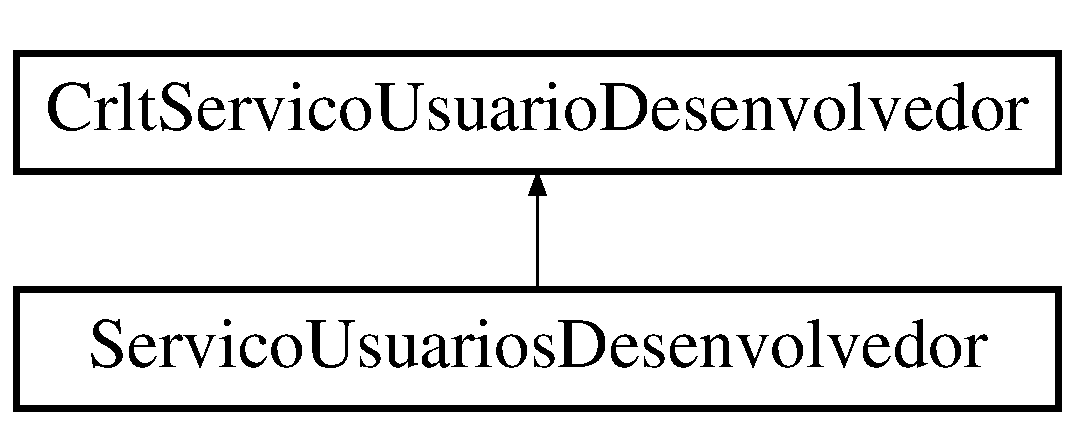
\includegraphics[height=2.000000cm]{class_servico_usuarios_desenvolvedor}
\end{center}
\end{figure}
\subsection*{Membros Públicos}
\begin{DoxyCompactItemize}
\item 
void \mbox{\hyperlink{class_servico_usuarios_desenvolvedor_a0214220e4cbac89da4ca22b10ac57c4e}{opcao\+Escolhida\+Desenvolvedor}} (int opcao, string email)
\item 
int \mbox{\hyperlink{class_servico_usuarios_desenvolvedor_a552cca1c14e7c9dd87600062d524ffa8}{consultar\+Cadastro\+Desenvolvedor}} (string email)
\item 
void \mbox{\hyperlink{class_servico_usuarios_desenvolvedor_ad536645995beed517216ed96206ae018}{excluir\+Usuario\+Desenvolvedor}} (string email)
\item 
void \mbox{\hyperlink{class_servico_usuarios_desenvolvedor_a2dc1811265f101d3ce14150594b25e88}{atualizar\+Usuario\+Desenvolvedor}} (string email)
\item 
void \mbox{\hyperlink{class_servico_usuarios_desenvolvedor_ad4f1b230cdb25ff8a2b8ae0010e99382}{list\+Nome\+Vocabularios}} ()
\item 
void \mbox{\hyperlink{class_servico_usuarios_desenvolvedor_a5748ea9d0e56ffcad31ad486ecb8b79f}{list\+Dados\+Vocabulario}} ()
\item 
void \mbox{\hyperlink{class_servico_usuarios_desenvolvedor_a9c4a519147798c77d3fb6406f8078b9f}{consultar\+Termo}} ()
\item 
void \mbox{\hyperlink{class_servico_usuarios_desenvolvedor_aa125405f5b747e4e7bbacebd28934e72}{consultar\+Definicao\+Termo}} ()
\item 
void \mbox{\hyperlink{class_servico_usuarios_desenvolvedor_a1708877c02739b2447862b2e2349267d}{cadastra\+Desenvolvedor\+Voc\+Controlado}} (string email)
\item 
void \mbox{\hyperlink{class_servico_usuarios_desenvolvedor_ab378812b1e6b4d648fb8860cf8444210}{cria\+Termo}} ()
\item 
void \mbox{\hyperlink{class_servico_usuarios_desenvolvedor_afb392520e6ea1209abb42ad0327673e0}{editar\+Termo}} ()
\item 
void \mbox{\hyperlink{class_servico_usuarios_desenvolvedor_a20712917886eaf28a2a9b308d14d7b04}{excluir\+Termo}} ()
\item 
void \mbox{\hyperlink{class_servico_usuarios_desenvolvedor_a851c2a4b054df2a14f66c451f4656d52}{cria\+Definicao}} ()
\item 
void \mbox{\hyperlink{class_servico_usuarios_desenvolvedor_a422f9a3ee77a0d560858c9f7c266b9ee}{excluir\+Definicao}} ()
\item 
void \mbox{\hyperlink{class_servico_usuarios_desenvolvedor_a2a1063014d21344c6ec9a101741e5a4e}{editar\+Definicao}} ()
\end{DoxyCompactItemize}


\subsection{Funções membros}
\mbox{\Hypertarget{class_servico_usuarios_desenvolvedor_a2dc1811265f101d3ce14150594b25e88}\label{class_servico_usuarios_desenvolvedor_a2dc1811265f101d3ce14150594b25e88}} 
\index{Servico\+Usuarios\+Desenvolvedor@{Servico\+Usuarios\+Desenvolvedor}!atualizar\+Usuario\+Desenvolvedor@{atualizar\+Usuario\+Desenvolvedor}}
\index{atualizar\+Usuario\+Desenvolvedor@{atualizar\+Usuario\+Desenvolvedor}!Servico\+Usuarios\+Desenvolvedor@{Servico\+Usuarios\+Desenvolvedor}}
\subsubsection{\texorpdfstring{atualizar\+Usuario\+Desenvolvedor()}{atualizarUsuarioDesenvolvedor()}}
{\footnotesize\ttfamily void Servico\+Usuarios\+Desenvolvedor\+::atualizar\+Usuario\+Desenvolvedor (\begin{DoxyParamCaption}\item[{string}]{email }\end{DoxyParamCaption})\hspace{0.3cm}{\ttfamily [virtual]}}

Nesse processo, similar ao do cadastro, todas as informacoes do desenvolvedor terao de ser atualizadas, nem que seja para coloca-\/las iguais, porem irao mesmo assim passar por uma nova validacao antes de serem gravadas no DB

Implementa \mbox{\hyperlink{class_crlt_servico_usuario_desenvolvedor_a63705805bc01450509e7719e2a57b1da}{Crlt\+Servico\+Usuario\+Desenvolvedor}}.


\begin{DoxyCode}
656 \{
662   \mbox{\hyperlink{class_sobrenome}{Sobrenome}} *sobrenome = \textcolor{keyword}{new} \mbox{\hyperlink{class_sobrenome}{Sobrenome}}();
663   \mbox{\hyperlink{class_email}{Email}} *emailAtualiza = \textcolor{keyword}{new} \mbox{\hyperlink{class_email}{Email}}();
664   \mbox{\hyperlink{class_data}{Data}} *data = \textcolor{keyword}{new} \mbox{\hyperlink{class_data}{Data}}();
665   \mbox{\hyperlink{class_senha}{Senha}} *senha = \textcolor{keyword}{new} \mbox{\hyperlink{class_senha}{Senha}}();
666   \mbox{\hyperlink{class_nome}{Nome}} *nome = \textcolor{keyword}{new} \mbox{\hyperlink{class_nome}{Nome}}();
667   \textcolor{comment}{//Leitor *leitor = new Leitor();}
668   \textcolor{keywordtype}{string} entrada;
669   \textcolor{keywordtype}{int} recebe;
670   \textcolor{keywordflow}{while}(\textcolor{keyword}{true})
671   \{
672       \textcolor{keywordflow}{try}
673       \{
674         cout << \textcolor{stringliteral}{"Nome: "};
675         cin >> entrada;
676         nome->\mbox{\hyperlink{class_nome_a83b9f56ec9f86f4b976846f4c5c65b30}{setNome}}(entrada);
677         \textcolor{comment}{//leitor->setNome(nome);}
678 
679         cout << \textcolor{stringliteral}{"Sobrenome: "};
680         cin >> entrada;
681         sobrenome->\mbox{\hyperlink{class_sobrenome_a9dc2277e3600656838e47c86dfddd23a}{setSobrenome}}(entrada);
682 
683         cout << \textcolor{stringliteral}{"Data de Nascimento: "};
684         cin >> entrada;
685         data->\mbox{\hyperlink{class_data_a5245638838a033c98a8b760836dddb7d}{setData}}(entrada);
686 
687         cout << \textcolor{stringliteral}{"Email: "};
688         cin >> entrada;
689         emailAtualiza->\mbox{\hyperlink{class_email_a2614b3a19d961411d1bece9c1bdf616f}{setEmail}}(entrada);
690 
691         cout << \textcolor{stringliteral}{"Senha: "};
692         cin >> entrada;
693         senha->\mbox{\hyperlink{class_senha_a01bbc2a82c5f405b68f33fe0dc538ec1}{setSenha}}(entrada,nome);
694 
695         \textcolor{keywordflow}{break};
696       \}
697       \textcolor{keywordflow}{catch}(\textcolor{keyword}{const} \textcolor{keywordtype}{char} *erro)
698       \{
699         cout << erro << endl;
700       \}
701     \}
702 
703   queryAtualiza = \textcolor{stringliteral}{"update Leitores set nome = '"};
704   queryAtualiza += nome->\mbox{\hyperlink{class_nome_aad41176173eec20cbbae1576447a3697}{getNome}}();
705   queryAtualiza += \textcolor{stringliteral}{"',sobrenome = '"};
706   queryAtualiza += sobrenome->\mbox{\hyperlink{class_sobrenome_a954491366ce07f6715f32a97d67edf04}{getSobrenome}}();
707   queryAtualiza += \textcolor{stringliteral}{"',data = '"};
708   queryAtualiza += data->\mbox{\hyperlink{class_data_afc7b15a5e81334858e48709b2f45cdc3}{getData}}();
709   queryAtualiza += \textcolor{stringliteral}{"',email = '"};
710   queryAtualiza += emailAtualiza->\mbox{\hyperlink{class_email_aa9a0e1a66b4efde65cf017bdd1c6c625}{getEmail}}();
711   queryAtualiza += \textcolor{stringliteral}{"',senha = '"};
712   queryAtualiza += senha->\mbox{\hyperlink{class_senha_a8786b3d03b1652e73df1cdce46cbbaaf}{getSenha}}();
713   queryAtualiza += \textcolor{stringliteral}{"' where email = '"};
714   queryAtualiza += email;
715   queryAtualiza += \textcolor{stringliteral}{"';"};
716 
717   \mbox{\hyperlink{comando_sql_8cpp_a4f89ddcbc4cf8f2587d89f72f8c7900d}{conectarDbUsuario}}();
718   recebe = \mbox{\hyperlink{comando_sql_8cpp_a748197580e7f9acdbf48c78de1f7924b}{executDbUsuario}}(queryAtualiza);
719   \mbox{\hyperlink{comando_sql_8cpp_a969be9911913568e30d4ae8963338bc3}{desconectarDbUsuario}}();
720 
721   cout <<\textcolor{stringliteral}{"QUERY: "} << queryAtualiza << endl;
722 \}
\end{DoxyCode}
\mbox{\Hypertarget{class_servico_usuarios_desenvolvedor_a1708877c02739b2447862b2e2349267d}\label{class_servico_usuarios_desenvolvedor_a1708877c02739b2447862b2e2349267d}} 
\index{Servico\+Usuarios\+Desenvolvedor@{Servico\+Usuarios\+Desenvolvedor}!cadastra\+Desenvolvedor\+Voc\+Controlado@{cadastra\+Desenvolvedor\+Voc\+Controlado}}
\index{cadastra\+Desenvolvedor\+Voc\+Controlado@{cadastra\+Desenvolvedor\+Voc\+Controlado}!Servico\+Usuarios\+Desenvolvedor@{Servico\+Usuarios\+Desenvolvedor}}
\subsubsection{\texorpdfstring{cadastra\+Desenvolvedor\+Voc\+Controlado()}{cadastraDesenvolvedorVocControlado()}}
{\footnotesize\ttfamily void Servico\+Usuarios\+Desenvolvedor\+::cadastra\+Desenvolvedor\+Voc\+Controlado (\begin{DoxyParamCaption}\item[{string}]{email }\end{DoxyParamCaption})\hspace{0.3cm}{\ttfamily [virtual]}}

Nessa funcao, um novo desenvolvedor sera cadastrado. Para se cadastrar como desenvolvedor de um vocabulario controlado, primeiramente precisamos verificar se esse vocabulario existe, e é isso que o programa faz. Primeiramente ele executa uma query em busca desse vocabulario, achado esse vocabulario, o email do desenvolvedor e consultado na tabela desse vocabulario para verificar se ele ja nao possui cadastro. Nao possuindo cadastro, agora sim, uma query sera montada para realizar seu cadastro como desenvolvedor desse vocabulario

Implementa \mbox{\hyperlink{class_crlt_servico_usuario_desenvolvedor_a8eb6d3af46ac497a394882ef0fe32eb1}{Crlt\+Servico\+Usuario\+Desenvolvedor}}.


\begin{DoxyCode}
856 \{
865   \textcolor{keywordtype}{string} vocabulario;
866   \textcolor{keywordtype}{string} query;
867   \textcolor{keywordtype}{int} resultado;
868 
869       cout << \textcolor{stringliteral}{"Digite o nome do vocabulario controlado no qual deseja se cadastrar: "};
870       cin >> vocabulario;
871 
872       query = \textcolor{stringliteral}{"select count(*) from Vocabulario\_Controlado where nomeVocabulario = '"};
873       query += vocabulario;
874       query += \textcolor{stringliteral}{"';"};
875 
876 
877       \mbox{\hyperlink{comando_sql_8cpp_a4f89ddcbc4cf8f2587d89f72f8c7900d}{conectarDbUsuario}}();
878       resultado = \mbox{\hyperlink{comando_sql_8cpp_af54952694f2fa7d76f969fb74b853cb9}{executDbUsuarioRows}}(query);
879 
880       \textcolor{keywordflow}{if}(resultado == -1)
881       \{
882         \textcolor{keywordflow}{throw} \textcolor{stringliteral}{"Erro, Vocabulario Controlado nao encontrado\(\backslash\)n"};
883       \}
884 
885         query = \textcolor{stringliteral}{"select count(*) from Vocabulario\_Controlado where desenvolvedores = '"};
886         query += email;
887         query += \textcolor{stringliteral}{"';"};
888         resultado = \mbox{\hyperlink{comando_sql_8cpp_af54952694f2fa7d76f969fb74b853cb9}{executDbUsuarioRows}}(query);
889 
890         \textcolor{keywordflow}{if}(resultado != -1)
891         \{
892           \textcolor{keywordflow}{throw} \textcolor{stringliteral}{"Usuario ja possui cadastrado\(\backslash\)n"};
893         \}
894 
895 
896         query = \textcolor{stringliteral}{"select count(*) from Vocabulario\_Controlado where nome nomeVocabulario = '"};
897         query += vocabulario;
898         query += \textcolor{stringliteral}{"';"};
899 
900         resultado = \mbox{\hyperlink{comando_sql_8cpp_af54952694f2fa7d76f969fb74b853cb9}{executDbUsuarioRows}}(query);
901 
902         \textcolor{keywordflow}{if}(resultado >= 10)
903         \{
904           \textcolor{keywordflow}{throw} \textcolor{stringliteral}{"Numero de desenvolvedores esgotado para esse Vocabulario;\(\backslash\)n"};
905         \}
906 
907 
908 
909         query = \textcolor{stringliteral}{"insert into Vocabulario\_Controlado (nomeVocabulario, idioma, emailAdmin)"};
910         query += \textcolor{stringliteral}{"select nomeVocabulario, idioma, emailAdmin from Vocabulario\_Controlado where
       nomeVocabulario = '"};
911         query += vocabulario;
912         query += \textcolor{stringliteral}{"' and desenvolvedores = '-';"};
913 
914         resultado = \mbox{\hyperlink{comando_sql_8cpp_a748197580e7f9acdbf48c78de1f7924b}{executDbUsuario}}(query);
915 
916         query = \textcolor{stringliteral}{"update Vocabulario\_Controlado set desenvolvedores = '"};
917         query += email;
918         query += \textcolor{stringliteral}{"' where desenvolvedores is null and nomeVocabulario = '"};
919         query += vocabulario;
920         query += \textcolor{stringliteral}{"';"};
921 
922         resultado = \mbox{\hyperlink{comando_sql_8cpp_a748197580e7f9acdbf48c78de1f7924b}{executDbUsuario}}(query);
923 
924         cout << \textcolor{stringliteral}{"Processando comandos....\(\backslash\)n\(\backslash\)n"};
925 
926         query = \textcolor{stringliteral}{"select count(*) from Vocabulario\_Controlado where desenvolvedores = '"};
927         query += email;
928         query += \textcolor{stringliteral}{"';"};
929 
930           resultado = \mbox{\hyperlink{comando_sql_8cpp_af54952694f2fa7d76f969fb74b853cb9}{executDbUsuarioRows}}(query);
931 
932           \textcolor{keywordflow}{if}(resultado != -1)
933           \{
934             cout << \textcolor{stringliteral}{"Desenvolvedor adicionado com sucesso....\(\backslash\)n\(\backslash\)n"};
935           \}
936           \textcolor{keywordflow}{else}
937           \{
938             \textcolor{keywordflow}{throw} \textcolor{stringliteral}{"Erro na execução do comando\(\backslash\)n\(\backslash\)n"};
939           \}
940 
941 \}
\end{DoxyCode}
\mbox{\Hypertarget{class_servico_usuarios_desenvolvedor_a552cca1c14e7c9dd87600062d524ffa8}\label{class_servico_usuarios_desenvolvedor_a552cca1c14e7c9dd87600062d524ffa8}} 
\index{Servico\+Usuarios\+Desenvolvedor@{Servico\+Usuarios\+Desenvolvedor}!consultar\+Cadastro\+Desenvolvedor@{consultar\+Cadastro\+Desenvolvedor}}
\index{consultar\+Cadastro\+Desenvolvedor@{consultar\+Cadastro\+Desenvolvedor}!Servico\+Usuarios\+Desenvolvedor@{Servico\+Usuarios\+Desenvolvedor}}
\subsubsection{\texorpdfstring{consultar\+Cadastro\+Desenvolvedor()}{consultarCadastroDesenvolvedor()}}
{\footnotesize\ttfamily int Servico\+Usuarios\+Desenvolvedor\+::consultar\+Cadastro\+Desenvolvedor (\begin{DoxyParamCaption}\item[{string}]{email }\end{DoxyParamCaption})\hspace{0.3cm}{\ttfamily [virtual]}}

Utiliza uma query simples de pesquisa onde atraves do parametro passado pela funcao, consegue exibir na tela os dados do desenvolvedor logado

Implementa \mbox{\hyperlink{class_crlt_servico_usuario_desenvolvedor_ad0e0d85a9a4763960f021fca4cf36f29}{Crlt\+Servico\+Usuario\+Desenvolvedor}}.


\begin{DoxyCode}
519 \{
524   queryConsulta = \textcolor{stringliteral}{"select * from Desenvolvedores where email= '"};
525   queryConsulta += email;
526   queryConsulta += \textcolor{stringliteral}{"';"};
527   \mbox{\hyperlink{comando_sql_8cpp_a4f89ddcbc4cf8f2587d89f72f8c7900d}{conectarDbUsuario}}();
528 
529   cout << \textcolor{stringliteral}{"\(\backslash\)t\(\backslash\)t------------- Dados do Usuario -----------------\(\backslash\)n"};
530 
531   resultadoQueryUsuario = \mbox{\hyperlink{comando_sql_8cpp_af54952694f2fa7d76f969fb74b853cb9}{executDbUsuarioRows}}(queryConsulta);
532 
533   \mbox{\hyperlink{comando_sql_8cpp_a969be9911913568e30d4ae8963338bc3}{desconectarDbUsuario}}();
534 
535   \textcolor{keywordflow}{return} resultadoQueryUsuario;
536 \}
\end{DoxyCode}
\mbox{\Hypertarget{class_servico_usuarios_desenvolvedor_aa125405f5b747e4e7bbacebd28934e72}\label{class_servico_usuarios_desenvolvedor_aa125405f5b747e4e7bbacebd28934e72}} 
\index{Servico\+Usuarios\+Desenvolvedor@{Servico\+Usuarios\+Desenvolvedor}!consultar\+Definicao\+Termo@{consultar\+Definicao\+Termo}}
\index{consultar\+Definicao\+Termo@{consultar\+Definicao\+Termo}!Servico\+Usuarios\+Desenvolvedor@{Servico\+Usuarios\+Desenvolvedor}}
\subsubsection{\texorpdfstring{consultar\+Definicao\+Termo()}{consultarDefinicaoTermo()}}
{\footnotesize\ttfamily void Servico\+Usuarios\+Desenvolvedor\+::consultar\+Definicao\+Termo (\begin{DoxyParamCaption}{ }\end{DoxyParamCaption})\hspace{0.3cm}{\ttfamily [virtual]}}



Implementa \mbox{\hyperlink{class_crlt_servico_usuario_desenvolvedor_acde5327b99fb4357276c4b0ab83fa20b}{Crlt\+Servico\+Usuario\+Desenvolvedor}}.


\begin{DoxyCode}
818 \{
819   \textcolor{keywordtype}{string} nomeTermo;
820   \textcolor{keywordtype}{string} queryVerifica;
821   \textcolor{keywordtype}{int} recebe;
822 
823   cout << \textcolor{stringliteral}{"Digite o nome do Termo no qual deseja consultar sua definicao: "};
824   cin >> nomeTermo;
825 
826 
827   queryVerifica = \textcolor{stringliteral}{"select count(*) from Termo inner join Definicao on Termo.nome = '"};
828   queryVerifica += nomeTermo;
829   queryVerifica += \textcolor{stringliteral}{"' and Definicao.termos = '"};
830   queryVerifica += nomeTermo;
831   queryVerifica += \textcolor{stringliteral}{"';"};
832 
833   cout << \textcolor{stringliteral}{"QUERY: "} <<  queryVerifica << endl;
834 
835   \mbox{\hyperlink{comando_sql_8cpp_a4f89ddcbc4cf8f2587d89f72f8c7900d}{conectarDbUsuario}}();
836   recebe = \mbox{\hyperlink{comando_sql_8cpp_af54952694f2fa7d76f969fb74b853cb9}{executDbUsuarioRows}}(queryVerifica);
837 
838   cout << \textcolor{stringliteral}{"VALOR: "} << recebe << endl;
839 
840   \textcolor{keywordflow}{if}(recebe > 0)
841   \{
842     queryVerifica = \textcolor{stringliteral}{"select texto from Definicao where termos = '"};
843     queryVerifica += nomeTermo;
844     queryVerifica += \textcolor{stringliteral}{"';"};
845     recebe = \mbox{\hyperlink{comando_sql_8cpp_a748197580e7f9acdbf48c78de1f7924b}{executDbUsuario}}(queryVerifica);
846   \}
847   \textcolor{keywordflow}{else}
848   \{
849     cout << \textcolor{stringliteral}{"Definicao para o termo "} << nomeTermo << \textcolor{stringliteral}{" nao foi encontrada"} << endl;
850   \}
851 
852   \mbox{\hyperlink{comando_sql_8cpp_a969be9911913568e30d4ae8963338bc3}{desconectarDbUsuario}}();
853 \}
\end{DoxyCode}
\mbox{\Hypertarget{class_servico_usuarios_desenvolvedor_a9c4a519147798c77d3fb6406f8078b9f}\label{class_servico_usuarios_desenvolvedor_a9c4a519147798c77d3fb6406f8078b9f}} 
\index{Servico\+Usuarios\+Desenvolvedor@{Servico\+Usuarios\+Desenvolvedor}!consultar\+Termo@{consultar\+Termo}}
\index{consultar\+Termo@{consultar\+Termo}!Servico\+Usuarios\+Desenvolvedor@{Servico\+Usuarios\+Desenvolvedor}}
\subsubsection{\texorpdfstring{consultar\+Termo()}{consultarTermo()}}
{\footnotesize\ttfamily void Servico\+Usuarios\+Desenvolvedor\+::consultar\+Termo (\begin{DoxyParamCaption}{ }\end{DoxyParamCaption})\hspace{0.3cm}{\ttfamily [virtual]}}

Primeiramente o nome do termo e pedido, e assim que colocado, uma pesquisa sera feita no DB em busca desse nome. Se o termo realmente existir, uma query sera criada para apresentar os dados desse termo, se nao, a funcao caira no catch

Implementa \mbox{\hyperlink{class_crlt_servico_usuario_desenvolvedor_a328f8ac2978c844ed4331d61ebfce32a}{Crlt\+Servico\+Usuario\+Desenvolvedor}}.


\begin{DoxyCode}
780 \{
786   \textcolor{keywordtype}{string} nomeTermo;
787   \textcolor{keywordtype}{string} queryVerifica;
788   \textcolor{keywordtype}{int} recebe;
789 
790   cout << \textcolor{stringliteral}{"Digite o nome do Termo que deseja consultar: "};
791   cin >> nomeTermo;
792 
793 
794   queryVerifica = \textcolor{stringliteral}{"select count(*) from Termo where nome = '"};
795   queryVerifica += nomeTermo;
796   queryVerifica += \textcolor{stringliteral}{"';"};
797 
798   \mbox{\hyperlink{comando_sql_8cpp_a4f89ddcbc4cf8f2587d89f72f8c7900d}{conectarDbUsuario}}();
799   recebe = \mbox{\hyperlink{comando_sql_8cpp_af54952694f2fa7d76f969fb74b853cb9}{executDbUsuarioRows}}(queryVerifica);
800 
801   \textcolor{keywordflow}{if}(recebe > 0)
802       \{
803         queryVerifica = \textcolor{stringliteral}{"select * from Termo where nome = '"};
804         queryVerifica += nomeTermo;
805         queryVerifica += \textcolor{stringliteral}{"';"};
806         recebe = \mbox{\hyperlink{comando_sql_8cpp_a748197580e7f9acdbf48c78de1f7924b}{executDbUsuario}}(queryVerifica);
807       \}
808   \textcolor{keywordflow}{else}
809       \{
810         cout << \textcolor{stringliteral}{"Termo nao consta em nosso banco de dados\(\backslash\)n"} << endl;
811       \}
812 
813       \mbox{\hyperlink{comando_sql_8cpp_a969be9911913568e30d4ae8963338bc3}{desconectarDbUsuario}}();
814 \}
\end{DoxyCode}
\mbox{\Hypertarget{class_servico_usuarios_desenvolvedor_a851c2a4b054df2a14f66c451f4656d52}\label{class_servico_usuarios_desenvolvedor_a851c2a4b054df2a14f66c451f4656d52}} 
\index{Servico\+Usuarios\+Desenvolvedor@{Servico\+Usuarios\+Desenvolvedor}!cria\+Definicao@{cria\+Definicao}}
\index{cria\+Definicao@{cria\+Definicao}!Servico\+Usuarios\+Desenvolvedor@{Servico\+Usuarios\+Desenvolvedor}}
\subsubsection{\texorpdfstring{cria\+Definicao()}{criaDefinicao()}}
{\footnotesize\ttfamily void Servico\+Usuarios\+Desenvolvedor\+::cria\+Definicao (\begin{DoxyParamCaption}{ }\end{DoxyParamCaption})\hspace{0.3cm}{\ttfamily [virtual]}}

Para criar uma definicao primeiramente e necessario verificar a qual termo ela ira se aplicar. informando o termo, esse mesmo sera chedado, e verificado se ele existe no banco de dados. Validando sua existencia o programa pedira para o usuario digitar sua definicao para esse termo, porem lembrando que se esse termo ja possuir definicao, elas serao contabilizadas, sendo 5 o numero maximo para definicoes de cada termo

Implementa \mbox{\hyperlink{class_crlt_servico_usuario_desenvolvedor_af9f1bd8b7ec576adb4bc2a8ac14e0905}{Crlt\+Servico\+Usuario\+Desenvolvedor}}.


\begin{DoxyCode}
1214 \{
1222   \textcolor{keywordtype}{string} query;
1223   \textcolor{keywordtype}{string} termo;
1224   \textcolor{keywordtype}{string} definicao;
1225   \textcolor{keywordtype}{int} resultado;
1226 
1227   cout << \textcolor{stringliteral}{"Digite o termo no qual deseja aplicar um definicao: "};
1228   cin >> termo;
1229   cin.ignore();
1230 
1231   \mbox{\hyperlink{comando_sql_8cpp_a4f89ddcbc4cf8f2587d89f72f8c7900d}{conectarDbUsuario}}();
1232 
1233   query = \textcolor{stringliteral}{"select count(*) from Termo where nome = '"};
1234   query += termo;
1235   query += \textcolor{stringliteral}{"';"};
1236 
1237   resultado = \mbox{\hyperlink{comando_sql_8cpp_af54952694f2fa7d76f969fb74b853cb9}{executDbUsuarioRows}}(query);
1238 
1239   \textcolor{keywordflow}{if}(resultado == -1)
1240   \{
1241     \textcolor{keywordflow}{throw} \textcolor{stringliteral}{"Erro, termo nao consta em nosso banco de dados\(\backslash\)n"};
1242   \}
1243 
1244   query = \textcolor{stringliteral}{"select count(*) from Definicao where termos = '"};
1245   query += termo;
1246   query += \textcolor{stringliteral}{"';"};
1247 
1248   resultado = \mbox{\hyperlink{comando_sql_8cpp_af54952694f2fa7d76f969fb74b853cb9}{executDbUsuarioRows}}(query);
1249 
1250   cout << \textcolor{stringliteral}{"Quantidade de termos retornados: "} << resultado << endl;
1251 
1252   \textcolor{keywordflow}{if}(resultado == 5)
1253   \{
1254     \textcolor{keywordflow}{throw} \textcolor{stringliteral}{"\(\backslash\)n\(\backslash\)tErro, termo ja possui numero maximo de definicoes\(\backslash\)n\(\backslash\)n"};
1255   \}
1256 
1257   cout << \textcolor{stringliteral}{"Digite a definicao para seu termo: "};
1258   getline(cin, definicao);
1259 
1260   query = \textcolor{stringliteral}{"insert into Definicao(texto, termos) "};
1261   query += \textcolor{stringliteral}{"values('"};
1262   query += definicao;
1263   query += \textcolor{stringliteral}{"','"};
1264   query += termo;
1265   query += \textcolor{stringliteral}{"');"};
1266 
1267   resultado = \mbox{\hyperlink{comando_sql_8cpp_a748197580e7f9acdbf48c78de1f7924b}{executDbUsuario}}(query);
1268 
1269   cout << \textcolor{stringliteral}{"\(\backslash\)t\(\backslash\)t ------------ Definicao aplicada com sucesso ------------------\(\backslash\)n\(\backslash\)n"};
1270 
1271   \mbox{\hyperlink{comando_sql_8cpp_a969be9911913568e30d4ae8963338bc3}{desconectarDbUsuario}}();
1272 
1273 \}
\end{DoxyCode}
\mbox{\Hypertarget{class_servico_usuarios_desenvolvedor_ab378812b1e6b4d648fb8860cf8444210}\label{class_servico_usuarios_desenvolvedor_ab378812b1e6b4d648fb8860cf8444210}} 
\index{Servico\+Usuarios\+Desenvolvedor@{Servico\+Usuarios\+Desenvolvedor}!cria\+Termo@{cria\+Termo}}
\index{cria\+Termo@{cria\+Termo}!Servico\+Usuarios\+Desenvolvedor@{Servico\+Usuarios\+Desenvolvedor}}
\subsubsection{\texorpdfstring{cria\+Termo()}{criaTermo()}}
{\footnotesize\ttfamily void Servico\+Usuarios\+Desenvolvedor\+::cria\+Termo (\begin{DoxyParamCaption}{ }\end{DoxyParamCaption})\hspace{0.3cm}{\ttfamily [virtual]}}

Primeiramente o programa pede para o usuario informar em qual vocabulario deseja cadastrar seu termo. Informando esse detalhe, uma pesquisa e feita em busca desse vocabulario. Achando esse vocabulario, e verificado se nele ja existe um termo com o mesmo nome, e se caso nao existe so assim que o novo termo podera ser cadastrado.

Implementa \mbox{\hyperlink{class_crlt_servico_usuario_desenvolvedor_a924f7dcd059d8ff265909d29457a961b}{Crlt\+Servico\+Usuario\+Desenvolvedor}}.


\begin{DoxyCode}
945 \{
952   \mbox{\hyperlink{class_nome}{Nome}} *nome = \textcolor{keyword}{new} \mbox{\hyperlink{class_nome}{Nome}}();
953   \mbox{\hyperlink{class_data}{Data}} *data = \textcolor{keyword}{new} \mbox{\hyperlink{class_data}{Data}}();
954   \mbox{\hyperlink{class_termo}{Termo}} *termo = \textcolor{keyword}{new} \mbox{\hyperlink{class_termo}{Termo}}();
955 \textcolor{keywordtype}{int} resultado;
956   \textcolor{keywordtype}{string} vocabulario;
957   \textcolor{keywordtype}{string} entrada;
958   \textcolor{keywordtype}{string} query;
959 
960   cout << \textcolor{stringliteral}{"Digite o nome do vocabulario no qual deseja que seu termo seja cadastrado: "};
961   cin >> vocabulario;
962   cin.ignore();
963 
964   query = \textcolor{stringliteral}{"select count(*) from Vocabulario\_Controlado where nomeVocabulario = '"};
965   query += vocabulario;
966   query += \textcolor{stringliteral}{"';"};
967 
968 
969   \mbox{\hyperlink{comando_sql_8cpp_a4f89ddcbc4cf8f2587d89f72f8c7900d}{conectarDbUsuario}}();
970   resultado = \mbox{\hyperlink{comando_sql_8cpp_af54952694f2fa7d76f969fb74b853cb9}{executDbUsuarioRows}}(query);
971 
972   \textcolor{keywordflow}{if}(resultado == -1)
973   \{
974     \textcolor{keywordflow}{throw} \textcolor{stringliteral}{"Erro, Vocabulario Controlado nao encontrado\(\backslash\)n"};
975   \}
976 \textcolor{keywordflow}{while}(\textcolor{keyword}{true})
977 \{
978   \textcolor{keywordflow}{try}
979   \{
980     cout << \textcolor{stringliteral}{"Nome do termo: "};
981     getline(cin, entrada);
982     nome->\mbox{\hyperlink{class_nome_a83b9f56ec9f86f4b976846f4c5c65b30}{setNome}}(entrada);
983     termo->\mbox{\hyperlink{class_termo_a43246196cccd6fa074731e93ac15f07a}{setNome}}(*nome);
984     query = \textcolor{stringliteral}{"select count(*) from Termo where nome = '"};
985     query += nome->\mbox{\hyperlink{class_nome_aad41176173eec20cbbae1576447a3697}{getNome}}();
986     query += \textcolor{stringliteral}{"';"};
987     resultado = \mbox{\hyperlink{comando_sql_8cpp_af54952694f2fa7d76f969fb74b853cb9}{executDbUsuarioRows}}(query);
988     \textcolor{keywordflow}{if}(resultado != -1)
989     \{
990       \textcolor{keywordflow}{throw} \textcolor{stringliteral}{"Erro, Termo ja consta em nosso banco de dados, tente outro Termo..\(\backslash\)n"};
991     \}
992 
993     cout << \textcolor{stringliteral}{"Classe do Termo: "};
994     getline(cin, entrada);
995     termo->\mbox{\hyperlink{class_termo_a8c32e501b39e008ea369650e3eb196b1}{setClasseDeTermo}}(entrada);
996 
997 
998     cout << \textcolor{stringliteral}{"Data da criacao: "};
999     cin >> entrada;
1000     data->\mbox{\hyperlink{class_data_a5245638838a033c98a8b760836dddb7d}{setData}}(entrada);
1001     termo->\mbox{\hyperlink{class_termo_abf829a90ed067a580bb9d4c90db0f160}{setData}}(*data);
1002 
1003     \textcolor{keywordflow}{break};
1004   \}
1005   \textcolor{keywordflow}{catch}(\textcolor{keyword}{const} \textcolor{keywordtype}{char} *erro)
1006   \{
1007     cout << erro << endl;
1008   \}
1009 \}
1010 
1011 
1012   query = \textcolor{stringliteral}{"insert into Termo (nome,classe,data,vocabulario)"};
1013   query += \textcolor{stringliteral}{"values('"};
1014   query += nome->\mbox{\hyperlink{class_nome_aad41176173eec20cbbae1576447a3697}{getNome}}();
1015   query += \textcolor{stringliteral}{"','"};
1016   query += termo->\mbox{\hyperlink{class_termo_ae7e8fb47c8e03506b98a952fa25aa97b}{getClasseDeTermo}}();
1017   query += \textcolor{stringliteral}{"','"};
1018   query += data->\mbox{\hyperlink{class_data_afc7b15a5e81334858e48709b2f45cdc3}{getData}}();
1019   query += \textcolor{stringliteral}{"','"};
1020   query += vocabulario;
1021   query += \textcolor{stringliteral}{"');"};
1022 
1023   resultado = \mbox{\hyperlink{comando_sql_8cpp_a748197580e7f9acdbf48c78de1f7924b}{executDbUsuario}}(query);
1024 
1025   query = \textcolor{stringliteral}{"select count(*)from Termo where nome = '"};
1026   query += nome->\mbox{\hyperlink{class_nome_aad41176173eec20cbbae1576447a3697}{getNome}}();
1027   query += \textcolor{stringliteral}{"';"};
1028 
1029   resultado = \mbox{\hyperlink{comando_sql_8cpp_af54952694f2fa7d76f969fb74b853cb9}{executDbUsuarioRows}}(query);
1030 
1031   \textcolor{keywordflow}{if}(resultado != -1)
1032   \{
1033     cout << \textcolor{stringliteral}{"Termo criado com sucesso...\(\backslash\)n\(\backslash\)n"};
1034   \}
1035   \textcolor{keywordflow}{else}
1036   \{
1037     \textcolor{keywordflow}{throw} \textcolor{stringliteral}{"Erro na criacao do Termo\(\backslash\)n\(\backslash\)n"};
1038   \}
1039 
1040   \mbox{\hyperlink{comando_sql_8cpp_a969be9911913568e30d4ae8963338bc3}{desconectarDbUsuario}}();
1041 \}
\end{DoxyCode}
\mbox{\Hypertarget{class_servico_usuarios_desenvolvedor_a2a1063014d21344c6ec9a101741e5a4e}\label{class_servico_usuarios_desenvolvedor_a2a1063014d21344c6ec9a101741e5a4e}} 
\index{Servico\+Usuarios\+Desenvolvedor@{Servico\+Usuarios\+Desenvolvedor}!editar\+Definicao@{editar\+Definicao}}
\index{editar\+Definicao@{editar\+Definicao}!Servico\+Usuarios\+Desenvolvedor@{Servico\+Usuarios\+Desenvolvedor}}
\subsubsection{\texorpdfstring{editar\+Definicao()}{editarDefinicao()}}
{\footnotesize\ttfamily void Servico\+Usuarios\+Desenvolvedor\+::editar\+Definicao (\begin{DoxyParamCaption}{ }\end{DoxyParamCaption})\hspace{0.3cm}{\ttfamily [virtual]}}

Para um definicao ser editada, primeiramente deve-\/se informar a qual termo pertence essa definicao logo apos validar esse termo, e necessario verificar se o mesmo apresenta alguma definicao. sendo apresentada alguma definicao, o usuario ira escolher a que deseja editar atraves do numero\+Def Colocado na definicao, para que possa alterar somente aquela que ele deseja.

Implementa \mbox{\hyperlink{class_crlt_servico_usuario_desenvolvedor_ae8e2d1d6954d5c4861d3cc40c525f725}{Crlt\+Servico\+Usuario\+Desenvolvedor}}.


\begin{DoxyCode}
1341  \{
1348    \textcolor{keywordtype}{string} query;
1349    \textcolor{keywordtype}{string} termo;
1350    \textcolor{keywordtype}{string} definicao;
1351    \textcolor{keywordtype}{string} numeroDef;
1352    \textcolor{keywordtype}{int} resultado;
1353 
1354    cout << \textcolor{stringliteral}{"Digite o nome do termo no qual deseja edita-lo: "};
1355    cin >> termo;
1356    cin.ignore();
1357 
1358 
1359 
1360    \mbox{\hyperlink{comando_sql_8cpp_a4f89ddcbc4cf8f2587d89f72f8c7900d}{conectarDbUsuario}}();
1361 
1362    query = \textcolor{stringliteral}{"select count(*) from Definicao where termos = '"};
1363    query += termo;
1364    query += \textcolor{stringliteral}{"';"};
1365 
1366    resultado = \mbox{\hyperlink{comando_sql_8cpp_af54952694f2fa7d76f969fb74b853cb9}{executDbUsuarioRows}}(query);
1367 
1368    \textcolor{keywordflow}{if}(resultado == -1)
1369    \{
1370      \textcolor{keywordflow}{throw} \textcolor{stringliteral}{"Erro, termo nao encontrado\(\backslash\)n\(\backslash\)n"};
1371    \}
1372 
1373    cout << \textcolor{stringliteral}{"\(\backslash\)t ---------- Apresentando definicoes do termo escolhido ----------\(\backslash\)n\(\backslash\)n"};
1374 
1375    query = \textcolor{stringliteral}{"select * from Definicao where termos = '"};
1376    query += termo;
1377    query += \textcolor{stringliteral}{"';"};
1378 
1379    resultado = \mbox{\hyperlink{comando_sql_8cpp_a748197580e7f9acdbf48c78de1f7924b}{executDbUsuario}}(query);
1380 
1381    cout << \textcolor{stringliteral}{"Digite o numero(numeroDef) apresentado na frente do termo no qual deseja editar: "};
1382    cin >> numeroDef;
1383    cin.ignore();
1384 
1385   cout << \textcolor{stringliteral}{"Digite a nova definicao para o termo escolhido: "};
1386   getline(cin, definicao);
1387 
1388   query = \textcolor{stringliteral}{"update Definicao set texto = '"};
1389   query += definicao;
1390   query +=  \textcolor{stringliteral}{"' where termos = '"};
1391   query += termo;
1392   query += \textcolor{stringliteral}{"' and numeroDef = "};
1393   query += numeroDef;
1394   query += \textcolor{stringliteral}{";"};
1395 
1396      resultado = \mbox{\hyperlink{comando_sql_8cpp_a748197580e7f9acdbf48c78de1f7924b}{executDbUsuario}}(query);
1397 
1398      query = \textcolor{stringliteral}{"select * from Definicao where numeroDef = "};
1399      query += numeroDef;
1400      query += \textcolor{stringliteral}{" and termos = '"};
1401      query += termo;
1402      query += \textcolor{stringliteral}{"';"};
1403 
1404      resultado = \mbox{\hyperlink{comando_sql_8cpp_a748197580e7f9acdbf48c78de1f7924b}{executDbUsuario}}(query);
1405 
1406      cout << \textcolor{stringliteral}{"Termo Editado com sucesso\(\backslash\)n\(\backslash\)n"};
1407 
1408      \mbox{\hyperlink{comando_sql_8cpp_a969be9911913568e30d4ae8963338bc3}{desconectarDbUsuario}}();
1409  \}
\end{DoxyCode}
\mbox{\Hypertarget{class_servico_usuarios_desenvolvedor_afb392520e6ea1209abb42ad0327673e0}\label{class_servico_usuarios_desenvolvedor_afb392520e6ea1209abb42ad0327673e0}} 
\index{Servico\+Usuarios\+Desenvolvedor@{Servico\+Usuarios\+Desenvolvedor}!editar\+Termo@{editar\+Termo}}
\index{editar\+Termo@{editar\+Termo}!Servico\+Usuarios\+Desenvolvedor@{Servico\+Usuarios\+Desenvolvedor}}
\subsubsection{\texorpdfstring{editar\+Termo()}{editarTermo()}}
{\footnotesize\ttfamily void Servico\+Usuarios\+Desenvolvedor\+::editar\+Termo (\begin{DoxyParamCaption}{ }\end{DoxyParamCaption})\hspace{0.3cm}{\ttfamily [virtual]}}

Primeiramente o programa pede ao usuario o nome do termo que deseja editar e esse e procurado no DB. O termo achado, instancias de objetos serao criadas, no qual essas compoe as informacoes do termo escolhido. Todas as informacoes terao que ser atualizadas e essas mesmas serao verificadas antes de serem salvas no DB

Implementa \mbox{\hyperlink{class_crlt_servico_usuario_desenvolvedor_a60098c3dd81dfb83ea03f4b7ace785dc}{Crlt\+Servico\+Usuario\+Desenvolvedor}}.


\begin{DoxyCode}
1045 \{
1052   \mbox{\hyperlink{class_nome}{Nome}} *nome = \textcolor{keyword}{new} \mbox{\hyperlink{class_nome}{Nome}}();
1053   \mbox{\hyperlink{class_data}{Data}} *data = \textcolor{keyword}{new} \mbox{\hyperlink{class_data}{Data}}();
1054   \mbox{\hyperlink{class_termo}{Termo}} *termo = \textcolor{keyword}{new} \mbox{\hyperlink{class_termo}{Termo}}();
1055   \textcolor{keywordtype}{string} termoEditar;
1056   \textcolor{keywordtype}{string} entrada;
1057   \textcolor{keywordtype}{string} query;
1058   \textcolor{keywordtype}{string} vocabulario;
1059   \textcolor{keywordtype}{int} resultado;
1060 
1061   cout << \textcolor{stringliteral}{"Digite o nome do termo que deseja editar: "};
1062   getline(cin, termoEditar);
1063   cin.ignore();
1064 
1065   \mbox{\hyperlink{comando_sql_8cpp_a4f89ddcbc4cf8f2587d89f72f8c7900d}{conectarDbUsuario}}();
1066 
1067   query = \textcolor{stringliteral}{"select count(*) from Termo where nome = '"};
1068   query += termoEditar;
1069   query += \textcolor{stringliteral}{"';"};
1070 
1071   resultado = \mbox{\hyperlink{comando_sql_8cpp_af54952694f2fa7d76f969fb74b853cb9}{executDbUsuarioRows}}(query);
1072 
1073   \textcolor{keywordflow}{if}(resultado == -1)
1074   \{
1075     \textcolor{keywordflow}{throw} \textcolor{stringliteral}{"Erro, termo nao encontrado\(\backslash\)n\(\backslash\)n"};
1076   \}
1077 
1078   cout << \textcolor{stringliteral}{"\(\backslash\)t\(\backslash\)t--------------- Digite os novos dados do termo -----------------\(\backslash\)n "};
1079 
1080   \textcolor{keywordflow}{while}(\textcolor{keyword}{true})
1081   \{
1082     \textcolor{keywordflow}{try}
1083     \{
1084       cout << \textcolor{stringliteral}{"Nome do termo: "};
1085       getline(cin, entrada);
1086       cin.ignore();
1087       nome->\mbox{\hyperlink{class_nome_a83b9f56ec9f86f4b976846f4c5c65b30}{setNome}}(entrada);
1088       termo->\mbox{\hyperlink{class_termo_a43246196cccd6fa074731e93ac15f07a}{setNome}}(*nome);
1089       query = \textcolor{stringliteral}{"select count(*) from Termo where nome = '"};
1090       query += nome->\mbox{\hyperlink{class_nome_aad41176173eec20cbbae1576447a3697}{getNome}}();
1091       query += \textcolor{stringliteral}{"';"};
1092       resultado = \mbox{\hyperlink{comando_sql_8cpp_af54952694f2fa7d76f969fb74b853cb9}{executDbUsuarioRows}}(query);
1093       \textcolor{keywordflow}{if}(resultado != -1)
1094       \{
1095         \textcolor{keywordflow}{throw} \textcolor{stringliteral}{"Erro, Termo ja consta em nosso banco de dados, tente outro Termo..\(\backslash\)n"};
1096       \}
1097 
1098       cout << \textcolor{stringliteral}{"Classe do Termo: "};
1099       getline(cin, entrada);
1100       cin.ignore();
1101       termo->\mbox{\hyperlink{class_termo_a8c32e501b39e008ea369650e3eb196b1}{setClasseDeTermo}}(entrada);
1102 
1103       cout << \textcolor{stringliteral}{"Data da criacao: "};
1104       cin >> entrada;
1105       cin.ignore();
1106       data->\mbox{\hyperlink{class_data_a5245638838a033c98a8b760836dddb7d}{setData}}(entrada);
1107       termo->\mbox{\hyperlink{class_termo_abf829a90ed067a580bb9d4c90db0f160}{setData}}(*data);
1108 
1109       cout << \textcolor{stringliteral}{"Vocabulario: "};
1110       cin >> vocabulario;
1111       query = \textcolor{stringliteral}{"select count(*) from Vocabulario\_Controlado where nomeVocabulario = '"};
1112       query += vocabulario;
1113       query += \textcolor{stringliteral}{"';"};
1114       resultado = \mbox{\hyperlink{comando_sql_8cpp_af54952694f2fa7d76f969fb74b853cb9}{executDbUsuarioRows}}(query);
1115       \textcolor{keywordflow}{if}(resultado == -1)
1116       \{
1117         \textcolor{keywordflow}{throw} \textcolor{stringliteral}{"Erro, Vocabulario nao encontrado, tente outro vocabulario....\(\backslash\)n"};
1118       \}
1119 
1120       \textcolor{keywordflow}{break};
1121     \}
1122     \textcolor{keywordflow}{catch}(\textcolor{keyword}{const} \textcolor{keywordtype}{char} *erro)
1123     \{
1124       cout << erro << endl;
1125     \}
1126   \}
1127 
1128     query = \textcolor{stringliteral}{"update Termo set nome = '"};
1129     query += nome->\mbox{\hyperlink{class_nome_aad41176173eec20cbbae1576447a3697}{getNome}}();
1130     query += \textcolor{stringliteral}{"',classe = '"};
1131     query += termo->\mbox{\hyperlink{class_termo_ae7e8fb47c8e03506b98a952fa25aa97b}{getClasseDeTermo}}();
1132     query += \textcolor{stringliteral}{"',data = '"};
1133     query += data->\mbox{\hyperlink{class_data_afc7b15a5e81334858e48709b2f45cdc3}{getData}}();
1134     query += \textcolor{stringliteral}{"', vocabulario = '"};
1135     query += vocabulario;
1136     query += \textcolor{stringliteral}{"' where nome = '"};
1137     query += termoEditar;
1138     query += \textcolor{stringliteral}{"';"};
1139 
1140     resultado = \mbox{\hyperlink{comando_sql_8cpp_a748197580e7f9acdbf48c78de1f7924b}{executDbUsuario}}(query);
1141 
1142     query = \textcolor{stringliteral}{"select count(*) from Termo where nome = '"};
1143     query += nome->\mbox{\hyperlink{class_nome_aad41176173eec20cbbae1576447a3697}{getNome}}();
1144     query += \textcolor{stringliteral}{"';"};
1145 
1146     resultado = \mbox{\hyperlink{comando_sql_8cpp_af54952694f2fa7d76f969fb74b853cb9}{executDbUsuarioRows}}(query);
1147 
1148     \textcolor{keywordflow}{if}(resultado != -1)
1149     \{
1150       cout << \textcolor{stringliteral}{"Comando executado com sucesso....\(\backslash\)n\(\backslash\)n"};
1151     \}
1152     \textcolor{keywordflow}{else}
1153     \{
1154       \textcolor{keywordflow}{throw} \textcolor{stringliteral}{"Erro ao executar comando\(\backslash\)n\(\backslash\)n"};
1155     \}
1156 
1157     \mbox{\hyperlink{comando_sql_8cpp_a969be9911913568e30d4ae8963338bc3}{desconectarDbUsuario}}();
1158 \}
\end{DoxyCode}
\mbox{\Hypertarget{class_servico_usuarios_desenvolvedor_a422f9a3ee77a0d560858c9f7c266b9ee}\label{class_servico_usuarios_desenvolvedor_a422f9a3ee77a0d560858c9f7c266b9ee}} 
\index{Servico\+Usuarios\+Desenvolvedor@{Servico\+Usuarios\+Desenvolvedor}!excluir\+Definicao@{excluir\+Definicao}}
\index{excluir\+Definicao@{excluir\+Definicao}!Servico\+Usuarios\+Desenvolvedor@{Servico\+Usuarios\+Desenvolvedor}}
\subsubsection{\texorpdfstring{excluir\+Definicao()}{excluirDefinicao()}}
{\footnotesize\ttfamily void Servico\+Usuarios\+Desenvolvedor\+::excluir\+Definicao (\begin{DoxyParamCaption}{ }\end{DoxyParamCaption})\hspace{0.3cm}{\ttfamily [virtual]}}

Para excluir a definicao de um termo, primeiro deve-\/se informar a qual termo ela pertence informando e validando essa informacao, o programa ira apresentar a Quantidade de definicoes existentes para o termo escolhido e junto com elas, um numero chamado de numero\+Def, utilizado para poder diferencia-\/las na hora da exclusao. O usuario ira selecionar aquela de deseja exluir atraves desse numero\+Def, executando por fim a query de exclusao.

Implementa \mbox{\hyperlink{class_crlt_servico_usuario_desenvolvedor_a518fe0443e450a73a7274b8dbef74a71}{Crlt\+Servico\+Usuario\+Desenvolvedor}}.


\begin{DoxyCode}
1277 \{
1285   \textcolor{keywordtype}{string} query;
1286   \textcolor{keywordtype}{int} resultado;
1287   \textcolor{keywordtype}{char} numeroDef;
1288   \textcolor{keywordtype}{string} termo;
1289 
1290   cout << \textcolor{stringliteral}{"Digite o termo no qual deseja excluir sua definicao: "};
1291   cin >> termo;
1292 
1293   query = \textcolor{stringliteral}{"select count(*) from Definicao where termos = '"};
1294   query += termo;
1295   query += \textcolor{stringliteral}{"';"};
1296 
1297   \mbox{\hyperlink{comando_sql_8cpp_a4f89ddcbc4cf8f2587d89f72f8c7900d}{conectarDbUsuario}}();
1298 
1299   resultado = \mbox{\hyperlink{comando_sql_8cpp_af54952694f2fa7d76f969fb74b853cb9}{executDbUsuarioRows}}(query);
1300 
1301   \textcolor{keywordflow}{if}(resultado == -1)
1302   \{
1303     \textcolor{keywordflow}{throw} \textcolor{stringliteral}{"Erro, termo nao existe em nosso banco de dados de definicoes\(\backslash\)n\(\backslash\)n"};
1304   \}
1305 
1306   cout << \textcolor{stringliteral}{"\(\backslash\)t\(\backslash\)t----------- Definicoes do Termo "} << termo << \textcolor{stringliteral}{"-----------\(\backslash\)n\(\backslash\)n"};
1307 
1308   query = \textcolor{stringliteral}{"select * from Definicao where termos = '"};
1309   query += termo;
1310   query += \textcolor{stringliteral}{"';"};
1311 
1312   resultado = \mbox{\hyperlink{comando_sql_8cpp_a748197580e7f9acdbf48c78de1f7924b}{executDbUsuario}}(query);
1313 
1314   cout << \textcolor{stringliteral}{"Digite o numero que representa a definicao do termo que deseja excluir: "};
1315   cin >> numeroDef;
1316 
1317   query = \textcolor{stringliteral}{"delete from Definicao where numeroDef = "};
1318   query += numeroDef;
1319   query += \textcolor{stringliteral}{" and termos = '"};
1320   query += termo;
1321   query += \textcolor{stringliteral}{"';"};
1322 
1323   cout << \textcolor{stringliteral}{"QUERYYY: "} << query << endl;
1324 
1325   resultado = \mbox{\hyperlink{comando_sql_8cpp_a748197580e7f9acdbf48c78de1f7924b}{executDbUsuario}}(query);
1326 
1327   cout << \textcolor{stringliteral}{"resultado exclusao\(\backslash\)n\(\backslash\)n"};
1328 
1329   query = \textcolor{stringliteral}{"select * from Definicao where termos = '"};
1330   query += termo;
1331   query += \textcolor{stringliteral}{"';"};
1332 
1333   resultado = \mbox{\hyperlink{comando_sql_8cpp_a748197580e7f9acdbf48c78de1f7924b}{executDbUsuario}}(query);
1334 
1335   \mbox{\hyperlink{comando_sql_8cpp_a969be9911913568e30d4ae8963338bc3}{desconectarDbUsuario}}();
1336 
1337 \}
\end{DoxyCode}
\mbox{\Hypertarget{class_servico_usuarios_desenvolvedor_a20712917886eaf28a2a9b308d14d7b04}\label{class_servico_usuarios_desenvolvedor_a20712917886eaf28a2a9b308d14d7b04}} 
\index{Servico\+Usuarios\+Desenvolvedor@{Servico\+Usuarios\+Desenvolvedor}!excluir\+Termo@{excluir\+Termo}}
\index{excluir\+Termo@{excluir\+Termo}!Servico\+Usuarios\+Desenvolvedor@{Servico\+Usuarios\+Desenvolvedor}}
\subsubsection{\texorpdfstring{excluir\+Termo()}{excluirTermo()}}
{\footnotesize\ttfamily void Servico\+Usuarios\+Desenvolvedor\+::excluir\+Termo (\begin{DoxyParamCaption}{ }\end{DoxyParamCaption})\hspace{0.3cm}{\ttfamily [virtual]}}

Primeiramente o nome do termo e pedido, e com isso comeca a procura dentro do DB. Achado o termo uma query sera montada e executada para que esse termo seja excluido do Banco de dados

Implementa \mbox{\hyperlink{class_crlt_servico_usuario_desenvolvedor_a95825708aeed4c1f6a5829ad4bd29673}{Crlt\+Servico\+Usuario\+Desenvolvedor}}.


\begin{DoxyCode}
1162 \{
1167   \textcolor{keywordtype}{string} query;
1168   \textcolor{keywordtype}{string} termo;
1169   \textcolor{keywordtype}{int} resultado;
1170 
1171   cout << \textcolor{stringliteral}{"Digite o nome do termo que deseja excluir: "};
1172   cin >> termo;
1173 
1174   query = \textcolor{stringliteral}{"select count(*) from Termo where nome = '"};
1175   query += termo;
1176   query += \textcolor{stringliteral}{"';"};
1177 
1178   \mbox{\hyperlink{comando_sql_8cpp_a4f89ddcbc4cf8f2587d89f72f8c7900d}{conectarDbUsuario}}();
1179 
1180   resultado = \mbox{\hyperlink{comando_sql_8cpp_af54952694f2fa7d76f969fb74b853cb9}{executDbUsuarioRows}}(query);
1181 
1182   \textcolor{keywordflow}{if}(resultado == -1)
1183   \{
1184     \textcolor{keywordflow}{throw} \textcolor{stringliteral}{"Erro, Termo nao encontrado\(\backslash\)n\(\backslash\)n"};
1185   \}
1186 
1187   query = \textcolor{stringliteral}{"delete from Termo where nome = '"};
1188   query += termo;
1189   query += \textcolor{stringliteral}{"';"};
1190 
1191   resultado = \mbox{\hyperlink{comando_sql_8cpp_a748197580e7f9acdbf48c78de1f7924b}{executDbUsuario}}(query);
1192 
1193   query = \textcolor{stringliteral}{"select count(*) from Termo where nome = '"};
1194   query += termo;
1195   query += \textcolor{stringliteral}{"';"};
1196 
1197   resultado = \mbox{\hyperlink{comando_sql_8cpp_af54952694f2fa7d76f969fb74b853cb9}{executDbUsuarioRows}}(query);
1198 
1199   \textcolor{keywordflow}{if}(resultado != -1)
1200   \{
1201     \textcolor{keywordflow}{throw} \textcolor{stringliteral}{"Erro na exclusao\(\backslash\)n\(\backslash\)n"};
1202   \}
1203   \textcolor{keywordflow}{else}
1204   \{
1205     cout << \textcolor{stringliteral}{"Exclusao de termo realizada com sucesso\(\backslash\)n\(\backslash\)n"};
1206   \}
1207 
1208   \mbox{\hyperlink{comando_sql_8cpp_a969be9911913568e30d4ae8963338bc3}{desconectarDbUsuario}}();
1209 
1210 \}
\end{DoxyCode}
\mbox{\Hypertarget{class_servico_usuarios_desenvolvedor_ad536645995beed517216ed96206ae018}\label{class_servico_usuarios_desenvolvedor_ad536645995beed517216ed96206ae018}} 
\index{Servico\+Usuarios\+Desenvolvedor@{Servico\+Usuarios\+Desenvolvedor}!excluir\+Usuario\+Desenvolvedor@{excluir\+Usuario\+Desenvolvedor}}
\index{excluir\+Usuario\+Desenvolvedor@{excluir\+Usuario\+Desenvolvedor}!Servico\+Usuarios\+Desenvolvedor@{Servico\+Usuarios\+Desenvolvedor}}
\subsubsection{\texorpdfstring{excluir\+Usuario\+Desenvolvedor()}{excluirUsuarioDesenvolvedor()}}
{\footnotesize\ttfamily void Servico\+Usuarios\+Desenvolvedor\+::excluir\+Usuario\+Desenvolvedor (\begin{DoxyParamCaption}\item[{string}]{email }\end{DoxyParamCaption})\hspace{0.3cm}{\ttfamily [virtual]}}

Atraves do parametro recebido pela funcao, uma query de delete e montada usando como criterio o email passado no parametro para poder assim excluir a conta do desenvolvedor logado

Implementa \mbox{\hyperlink{class_crlt_servico_usuario_desenvolvedor_aa106326b5823377bd842b7448e0b4ee3}{Crlt\+Servico\+Usuario\+Desenvolvedor}}.


\begin{DoxyCode}
631 \{
636   \textcolor{keywordtype}{int} consulta,recebe;
637   queryExclui = \textcolor{stringliteral}{"delete from Desenvolvedores where email='"};
638   queryExclui += email;
639   queryExclui +=\textcolor{stringliteral}{"';"};
640 
641   \mbox{\hyperlink{class_servico_usuarios_desenvolvedor_a552cca1c14e7c9dd87600062d524ffa8}{consultarCadastroDesenvolvedor}}(email);
642 
643   \textcolor{keywordflow}{if}(consulta == 0)
644   \{
645     \textcolor{keywordflow}{throw} \textcolor{stringliteral}{"Erro, cadastro nao existe em nosso banco de dados\(\backslash\)n"};
646   \}
647 
648   cout << queryExclui << endl;
649 
650   \mbox{\hyperlink{comando_sql_8cpp_a4f89ddcbc4cf8f2587d89f72f8c7900d}{conectarDbUsuario}}();
651   recebe = \mbox{\hyperlink{comando_sql_8cpp_a748197580e7f9acdbf48c78de1f7924b}{executDbUsuario}}(queryExclui);
652   \mbox{\hyperlink{comando_sql_8cpp_a969be9911913568e30d4ae8963338bc3}{desconectarDbUsuario}}();
653 \}
\end{DoxyCode}
\mbox{\Hypertarget{class_servico_usuarios_desenvolvedor_a5748ea9d0e56ffcad31ad486ecb8b79f}\label{class_servico_usuarios_desenvolvedor_a5748ea9d0e56ffcad31ad486ecb8b79f}} 
\index{Servico\+Usuarios\+Desenvolvedor@{Servico\+Usuarios\+Desenvolvedor}!list\+Dados\+Vocabulario@{list\+Dados\+Vocabulario}}
\index{list\+Dados\+Vocabulario@{list\+Dados\+Vocabulario}!Servico\+Usuarios\+Desenvolvedor@{Servico\+Usuarios\+Desenvolvedor}}
\subsubsection{\texorpdfstring{list\+Dados\+Vocabulario()}{listDadosVocabulario()}}
{\footnotesize\ttfamily void Servico\+Usuarios\+Desenvolvedor\+::list\+Dados\+Vocabulario (\begin{DoxyParamCaption}{ }\end{DoxyParamCaption})\hspace{0.3cm}{\ttfamily [virtual]}}

Primeiramente o nome do vocabulario controlado e pedido, e assim que colocado, uma pesquisa sera feita no DB em busca desse nome. Se vocabulario realmente existir, uma query sera criada para apresentar os dados desse vocabulario, se nao, a funcao caira no catch

Implementa \mbox{\hyperlink{class_crlt_servico_usuario_desenvolvedor_a8fb9d062db341aa57ee44ff7b5049652}{Crlt\+Servico\+Usuario\+Desenvolvedor}}.


\begin{DoxyCode}
743 \{
749   \textcolor{keywordtype}{string} nomeVocabulario;
750   \textcolor{keywordtype}{string} queryVerifica;
751   \textcolor{keywordtype}{int} recebe;
752 
753   cout << \textcolor{stringliteral}{"Digite o nome do vocabulario desejado: "};
754   cin >> nomeVocabulario;
755 
756 
757   queryVerifica = \textcolor{stringliteral}{"select count(*) from Vocabulario\_Controlado where nomeVocabulario = '"};
758   queryVerifica += nomeVocabulario;
759   queryVerifica += \textcolor{stringliteral}{"';"};
760 
761   \mbox{\hyperlink{comando_sql_8cpp_a4f89ddcbc4cf8f2587d89f72f8c7900d}{conectarDbUsuario}}();
762   recebe = \mbox{\hyperlink{comando_sql_8cpp_af54952694f2fa7d76f969fb74b853cb9}{executDbUsuarioRows}}(queryVerifica);
763 
764   \textcolor{keywordflow}{if}(recebe > 0)
765       \{
766         queryVerifica = \textcolor{stringliteral}{"select * from Vocabulario\_Controlado where nomeVocabulario = '"};
767         queryVerifica += nomeVocabulario;
768         queryVerifica += \textcolor{stringliteral}{"';"};
769         recebe = \mbox{\hyperlink{comando_sql_8cpp_a748197580e7f9acdbf48c78de1f7924b}{executDbUsuario}}(queryVerifica);
770       \}
771   \textcolor{keywordflow}{else}
772       \{
773         cout << \textcolor{stringliteral}{"\(\backslash\)nVocabulario Controlado nao consta em nosso banco de dados\(\backslash\)n"} << endl;
774       \}
775 
776       \mbox{\hyperlink{comando_sql_8cpp_a969be9911913568e30d4ae8963338bc3}{desconectarDbUsuario}}();
777 \}
\end{DoxyCode}
\mbox{\Hypertarget{class_servico_usuarios_desenvolvedor_ad4f1b230cdb25ff8a2b8ae0010e99382}\label{class_servico_usuarios_desenvolvedor_ad4f1b230cdb25ff8a2b8ae0010e99382}} 
\index{Servico\+Usuarios\+Desenvolvedor@{Servico\+Usuarios\+Desenvolvedor}!list\+Nome\+Vocabularios@{list\+Nome\+Vocabularios}}
\index{list\+Nome\+Vocabularios@{list\+Nome\+Vocabularios}!Servico\+Usuarios\+Desenvolvedor@{Servico\+Usuarios\+Desenvolvedor}}
\subsubsection{\texorpdfstring{list\+Nome\+Vocabularios()}{listNomeVocabularios()}}
{\footnotesize\ttfamily void Servico\+Usuarios\+Desenvolvedor\+::list\+Nome\+Vocabularios (\begin{DoxyParamCaption}{ }\end{DoxyParamCaption})\hspace{0.3cm}{\ttfamily [virtual]}}

Lista todos os nomes dos vocabularios controlados ja cadastrados atraves da execucao de uma query

Implementa \mbox{\hyperlink{class_crlt_servico_usuario_desenvolvedor_abb3f10c499ac67d02987f0860150393d}{Crlt\+Servico\+Usuario\+Desenvolvedor}}.


\begin{DoxyCode}
726 \{
730   \textcolor{keywordtype}{string} queryList;
731   \textcolor{keywordtype}{int} recebe;
732   queryList = \textcolor{stringliteral}{"select nomeVocabulario from Vocabulario\_Controlado;"};
733   \mbox{\hyperlink{comando_sql_8cpp_a4f89ddcbc4cf8f2587d89f72f8c7900d}{conectarDbUsuario}}();
734   recebe = \mbox{\hyperlink{comando_sql_8cpp_a748197580e7f9acdbf48c78de1f7924b}{executDbUsuario}}(queryList);
735   \textcolor{keywordflow}{if}(recebe == 0)
736   \{
737     cout << \textcolor{stringliteral}{"Erro ao executar query\(\backslash\)n"};
738   \}
739   \mbox{\hyperlink{comando_sql_8cpp_a969be9911913568e30d4ae8963338bc3}{desconectarDbUsuario}}();
740 \}
\end{DoxyCode}
\mbox{\Hypertarget{class_servico_usuarios_desenvolvedor_a0214220e4cbac89da4ca22b10ac57c4e}\label{class_servico_usuarios_desenvolvedor_a0214220e4cbac89da4ca22b10ac57c4e}} 
\index{Servico\+Usuarios\+Desenvolvedor@{Servico\+Usuarios\+Desenvolvedor}!opcao\+Escolhida\+Desenvolvedor@{opcao\+Escolhida\+Desenvolvedor}}
\index{opcao\+Escolhida\+Desenvolvedor@{opcao\+Escolhida\+Desenvolvedor}!Servico\+Usuarios\+Desenvolvedor@{Servico\+Usuarios\+Desenvolvedor}}
\subsubsection{\texorpdfstring{opcao\+Escolhida\+Desenvolvedor()}{opcaoEscolhidaDesenvolvedor()}}
{\footnotesize\ttfamily void Servico\+Usuarios\+Desenvolvedor\+::opcao\+Escolhida\+Desenvolvedor (\begin{DoxyParamCaption}\item[{int}]{opcao,  }\item[{string}]{email }\end{DoxyParamCaption})}


\begin{DoxyCode}
2517 \{
2518   \textcolor{keywordflow}{if}(opcao == 1)
2519   \{
2520     \textcolor{keywordtype}{int} recebe;
2521       recebe = \mbox{\hyperlink{class_servico_usuarios_desenvolvedor_a552cca1c14e7c9dd87600062d524ffa8}{consultarCadastroDesenvolvedor}}(email);
2522   \}
2523 
2524   \textcolor{keywordflow}{if}(opcao == 2)
2525   \{
2526     \mbox{\hyperlink{class_servico_usuarios_desenvolvedor_a2dc1811265f101d3ce14150594b25e88}{atualizarUsuarioDesenvolvedor}}(email);
2527   \}
2528 
2529   \textcolor{keywordflow}{if}(opcao == 3)
2530   \{
2531     \mbox{\hyperlink{class_servico_usuarios_desenvolvedor_ad536645995beed517216ed96206ae018}{excluirUsuarioDesenvolvedor}}(email);
2532   \}
2533 
2534   \textcolor{keywordflow}{if}(opcao == 4)
2535   \{
2536     \mbox{\hyperlink{class_servico_usuarios_desenvolvedor_ad4f1b230cdb25ff8a2b8ae0010e99382}{listNomeVocabularios}}();
2537   \}
2538 
2539   \textcolor{keywordflow}{if}(opcao == 5)
2540   \{
2541     \mbox{\hyperlink{class_servico_usuarios_desenvolvedor_a5748ea9d0e56ffcad31ad486ecb8b79f}{listDadosVocabulario}}();
2542   \}
2543 
2544   \textcolor{keywordflow}{if}(opcao == 6)
2545   \{
2546     \mbox{\hyperlink{class_servico_usuarios_desenvolvedor_a9c4a519147798c77d3fb6406f8078b9f}{consultarTermo}}();
2547   \}
2548 
2549   \textcolor{keywordflow}{if}(opcao == 7)
2550   \{
2551     \mbox{\hyperlink{class_servico_usuarios_desenvolvedor_aa125405f5b747e4e7bbacebd28934e72}{consultarDefinicaoTermo}}();
2552   \}
2553 
2554   \textcolor{keywordflow}{if}(opcao == 8)
2555   \{
2556     \textcolor{keywordflow}{try}
2557     \{
2558       \mbox{\hyperlink{class_servico_usuarios_desenvolvedor_a1708877c02739b2447862b2e2349267d}{cadastraDesenvolvedorVocControlado}}(email);
2559     \}
2560     \textcolor{keywordflow}{catch}(\textcolor{keyword}{const} \textcolor{keywordtype}{char} *erro)
2561     \{
2562       cout << erro << endl;
2563     \}
2564   \}
2565 
2566   \textcolor{keywordflow}{if}(opcao == 9)
2567   \{
2568     \textcolor{keywordflow}{try}
2569     \{
2570       \mbox{\hyperlink{class_servico_usuarios_desenvolvedor_ab378812b1e6b4d648fb8860cf8444210}{criaTermo}}();
2571     \}
2572     \textcolor{keywordflow}{catch}(\textcolor{keyword}{const} \textcolor{keywordtype}{char} *erro)
2573     \{
2574       cout << erro << endl;
2575     \}
2576   \}
2577 
2578   \textcolor{keywordflow}{if}(opcao == 10)
2579   \{
2580     \textcolor{keywordflow}{try}
2581     \{
2582       \mbox{\hyperlink{class_servico_usuarios_desenvolvedor_afb392520e6ea1209abb42ad0327673e0}{editarTermo}}();
2583     \}
2584     \textcolor{keywordflow}{catch}(\textcolor{keyword}{const} \textcolor{keywordtype}{char} *erro)
2585     \{
2586       cout << erro << endl;
2587     \}
2588   \}
2589 
2590   \textcolor{keywordflow}{if}(opcao == 11)
2591   \{
2592     \textcolor{keywordflow}{try}
2593     \{
2594       \mbox{\hyperlink{class_servico_usuarios_desenvolvedor_a20712917886eaf28a2a9b308d14d7b04}{excluirTermo}}();
2595     \}
2596     \textcolor{keywordflow}{catch}(\textcolor{keyword}{const} \textcolor{keywordtype}{char} *erro)
2597     \{
2598       cout << erro << endl;
2599     \}
2600   \}
2601 
2602 
2603   \textcolor{keywordflow}{if}(opcao == 12)
2604   \{
2605     \textcolor{keywordflow}{try}
2606     \{
2607       \mbox{\hyperlink{class_servico_usuarios_desenvolvedor_a851c2a4b054df2a14f66c451f4656d52}{criaDefinicao}}();
2608     \}
2609     \textcolor{keywordflow}{catch}(\textcolor{keyword}{const} \textcolor{keywordtype}{char} *erro)
2610     \{
2611       cout << erro << endl;
2612     \}
2613   \}
2614 
2615 
2616   \textcolor{keywordflow}{if}(opcao == 13)
2617   \{
2618     \textcolor{keywordflow}{try}
2619     \{
2620       \mbox{\hyperlink{class_servico_usuarios_desenvolvedor_a422f9a3ee77a0d560858c9f7c266b9ee}{excluirDefinicao}}();
2621     \}
2622     \textcolor{keywordflow}{catch}(\textcolor{keyword}{const} \textcolor{keywordtype}{char} *erro)
2623     \{
2624       cout << erro << endl;
2625     \}
2626   \}
2627 
2628 
2629 
2630     \textcolor{keywordflow}{if}(opcao == 14)
2631     \{
2632       \textcolor{keywordflow}{try}
2633       \{
2634         \mbox{\hyperlink{class_servico_usuarios_desenvolvedor_a2a1063014d21344c6ec9a101741e5a4e}{editarDefinicao}}();
2635       \}
2636       \textcolor{keywordflow}{catch}(\textcolor{keyword}{const} \textcolor{keywordtype}{char} *erro)
2637       \{
2638         cout << erro << endl;
2639       \}
2640     \}
2641 
2642 \}
\end{DoxyCode}


A documentação para essa classe foi gerada a partir dos seguintes arquivos\+:\begin{DoxyCompactItemize}
\item 
/\+Users/amadeulinhares/\+Desktop/\+Trabalho3/\mbox{\hyperlink{servico_8hpp}{servico.\+hpp}}\item 
/\+Users/amadeulinhares/\+Desktop/\+Trabalho3/\mbox{\hyperlink{servico_8cpp}{servico.\+cpp}}\end{DoxyCompactItemize}

\hypertarget{class_servico_usuarios_leitor}{}\section{Referência da Classe Servico\+Usuarios\+Leitor}
\label{class_servico_usuarios_leitor}\index{Servico\+Usuarios\+Leitor@{Servico\+Usuarios\+Leitor}}


{\ttfamily \#include $<$servico.\+hpp$>$}

Diagrama de hierarquia para Servico\+Usuarios\+Leitor\+:\begin{figure}[H]
\begin{center}
\leavevmode
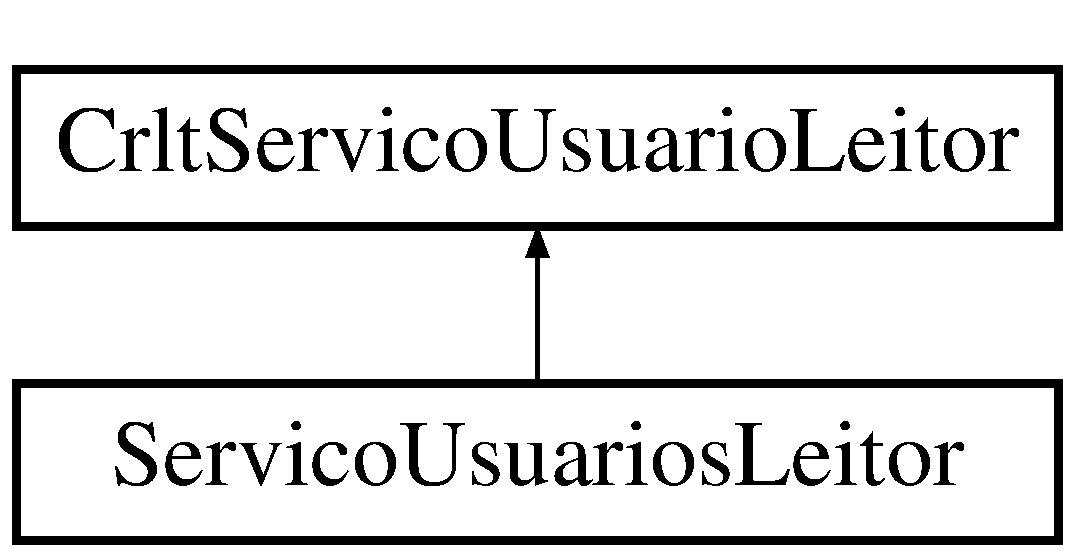
\includegraphics[height=2.000000cm]{class_servico_usuarios_leitor}
\end{center}
\end{figure}
\subsection*{Membros Públicos}
\begin{DoxyCompactItemize}
\item 
void \mbox{\hyperlink{class_servico_usuarios_leitor_a9a8e9ac18739ef8e75f670236ba90c20}{opcao\+Escolhida\+Leitor}} (int opcao, string email)
\item 
int \mbox{\hyperlink{class_servico_usuarios_leitor_a8f34dddc0540f729a701d69f948ffb42}{consultar\+Cadastro\+Leitor}} (string email)
\item 
void \mbox{\hyperlink{class_servico_usuarios_leitor_adce08fccebc11dbd5f395b8a4bb23d2a}{excluir\+Usuario\+Leitor}} (string email)
\item 
void \mbox{\hyperlink{class_servico_usuarios_leitor_ad77426aecdda591b99ecbf8259a05b2d}{atualizar\+Usuario\+Leitor}} (string email)
\item 
void \mbox{\hyperlink{class_servico_usuarios_leitor_a376f7cdbdea50d9a01ce611e79d346c4}{list\+Nome\+Vocabularios}} ()
\item 
void \mbox{\hyperlink{class_servico_usuarios_leitor_a4f533d318634c95d3f756a45c7613047}{list\+Dados\+Vocabulario}} ()
\item 
void \mbox{\hyperlink{class_servico_usuarios_leitor_a79d3a1814ad33930aae0c3a74c879e92}{consultar\+Termo}} ()
\item 
void \mbox{\hyperlink{class_servico_usuarios_leitor_a89ed39e45ee1c564e1f62df7154d1b29}{consultar\+Definicao\+Termo}} ()
\end{DoxyCompactItemize}


\subsection{Funções membros}
\mbox{\Hypertarget{class_servico_usuarios_leitor_ad77426aecdda591b99ecbf8259a05b2d}\label{class_servico_usuarios_leitor_ad77426aecdda591b99ecbf8259a05b2d}} 
\index{Servico\+Usuarios\+Leitor@{Servico\+Usuarios\+Leitor}!atualizar\+Usuario\+Leitor@{atualizar\+Usuario\+Leitor}}
\index{atualizar\+Usuario\+Leitor@{atualizar\+Usuario\+Leitor}!Servico\+Usuarios\+Leitor@{Servico\+Usuarios\+Leitor}}
\subsubsection{\texorpdfstring{atualizar\+Usuario\+Leitor()}{atualizarUsuarioLeitor()}}
{\footnotesize\ttfamily void Servico\+Usuarios\+Leitor\+::atualizar\+Usuario\+Leitor (\begin{DoxyParamCaption}\item[{string}]{email }\end{DoxyParamCaption})\hspace{0.3cm}{\ttfamily [virtual]}}

Essa funcao recebe com parametro o email do usuario logado no sistema. Ao executar essa Funcao o usuario logado tera que editar todos os dados de seu cadastro, sem opcao de escolha, e os novos dados tambem irao passar por uma verificacao antes de ocorrer a substituicao dos dados Apos a validacao das informacoes, uma query e montada e com isso os novos dados sao armazenados no banco de dados

Implementa \mbox{\hyperlink{class_crlt_servico_usuario_leitor_a075822102b4f3cbf1805507d8b78fde8}{Crlt\+Servico\+Usuario\+Leitor}}.


\begin{DoxyCode}
253 \{
262   \mbox{\hyperlink{class_nome}{Nome}} *nome = \textcolor{keyword}{new} \mbox{\hyperlink{class_nome}{Nome}}();
263   \mbox{\hyperlink{class_sobrenome}{Sobrenome}} *sobrenome = \textcolor{keyword}{new} \mbox{\hyperlink{class_sobrenome}{Sobrenome}}();
264   \mbox{\hyperlink{class_email}{Email}} *emailAtualiza = \textcolor{keyword}{new} \mbox{\hyperlink{class_email}{Email}}();
265   \mbox{\hyperlink{class_senha}{Senha}} *senha = \textcolor{keyword}{new} \mbox{\hyperlink{class_senha}{Senha}}();
266   \textcolor{comment}{//Leitor *leitor = new Leitor();}
267   \textcolor{keywordtype}{string} entrada;
268   \textcolor{keywordtype}{int} recebe;
269   \textcolor{keywordflow}{while}(\textcolor{keyword}{true})
270   \{
271       \textcolor{keywordflow}{try}
272       \{
273         cout << \textcolor{stringliteral}{"Nome: "};
274         cin >> entrada;
275         nome->\mbox{\hyperlink{class_nome_a83b9f56ec9f86f4b976846f4c5c65b30}{setNome}}(entrada);
276         \textcolor{comment}{//leitor->setNome(nome);}
277 
278         cout << \textcolor{stringliteral}{"Sobrenome: "};
279         cin >> entrada;
280         sobrenome->\mbox{\hyperlink{class_sobrenome_a9dc2277e3600656838e47c86dfddd23a}{setSobrenome}}(entrada);
281 
282         cout << \textcolor{stringliteral}{"Email: "};
283         cin >> entrada;
284         emailAtualiza->\mbox{\hyperlink{class_email_a2614b3a19d961411d1bece9c1bdf616f}{setEmail}}(entrada);
285 
286         cout << \textcolor{stringliteral}{"Senha: "};
287         cin >> entrada;
288         senha->\mbox{\hyperlink{class_senha_a01bbc2a82c5f405b68f33fe0dc538ec1}{setSenha}}(entrada,nome);
289 
290         \textcolor{keywordflow}{break};
291       \}
292       \textcolor{keywordflow}{catch}(\textcolor{keyword}{const} \textcolor{keywordtype}{char} *erro)
293       \{
294         cout << erro << endl;
295       \}
296     \}
297 
298   queryAtualiza = \textcolor{stringliteral}{"update Leitores set nome = '"};
299   queryAtualiza += nome->\mbox{\hyperlink{class_nome_aad41176173eec20cbbae1576447a3697}{getNome}}();
300   queryAtualiza += \textcolor{stringliteral}{"',sobrenome = '"};
301   queryAtualiza += sobrenome->\mbox{\hyperlink{class_sobrenome_a954491366ce07f6715f32a97d67edf04}{getSobrenome}}();
302   queryAtualiza += \textcolor{stringliteral}{"',email = '"};
303   queryAtualiza += emailAtualiza->\mbox{\hyperlink{class_email_aa9a0e1a66b4efde65cf017bdd1c6c625}{getEmail}}();
304   queryAtualiza += \textcolor{stringliteral}{"',senha = '"};
305   queryAtualiza += senha->\mbox{\hyperlink{class_senha_a8786b3d03b1652e73df1cdce46cbbaaf}{getSenha}}();
306   queryAtualiza += \textcolor{stringliteral}{"' where email = '"};
307   queryAtualiza += email;
308   queryAtualiza += \textcolor{stringliteral}{"';"};
309 
310   \mbox{\hyperlink{comando_sql_8cpp_a4f89ddcbc4cf8f2587d89f72f8c7900d}{conectarDbUsuario}}();
311   recebe = \mbox{\hyperlink{comando_sql_8cpp_a748197580e7f9acdbf48c78de1f7924b}{executDbUsuario}}(queryAtualiza);
312   \mbox{\hyperlink{comando_sql_8cpp_a969be9911913568e30d4ae8963338bc3}{desconectarDbUsuario}}();
313 
314 \}
\end{DoxyCode}
\mbox{\Hypertarget{class_servico_usuarios_leitor_a8f34dddc0540f729a701d69f948ffb42}\label{class_servico_usuarios_leitor_a8f34dddc0540f729a701d69f948ffb42}} 
\index{Servico\+Usuarios\+Leitor@{Servico\+Usuarios\+Leitor}!consultar\+Cadastro\+Leitor@{consultar\+Cadastro\+Leitor}}
\index{consultar\+Cadastro\+Leitor@{consultar\+Cadastro\+Leitor}!Servico\+Usuarios\+Leitor@{Servico\+Usuarios\+Leitor}}
\subsubsection{\texorpdfstring{consultar\+Cadastro\+Leitor()}{consultarCadastroLeitor()}}
{\footnotesize\ttfamily int Servico\+Usuarios\+Leitor\+::consultar\+Cadastro\+Leitor (\begin{DoxyParamCaption}\item[{string}]{email }\end{DoxyParamCaption})\hspace{0.3cm}{\ttfamily [virtual]}}

Funcao consiste em receber o email do leitor que logou no sistema e com isso executar uma query no qual os dados desse mesmo leitor serao apresentados na tela

Implementa \mbox{\hyperlink{class_crlt_servico_usuario_leitor_a4585305b98f21fe233b2c798edb47496}{Crlt\+Servico\+Usuario\+Leitor}}.


\begin{DoxyCode}
117 \{
123   queryConsulta = \textcolor{stringliteral}{"select * from Leitores where email= '"};
124   queryConsulta += email;
125   queryConsulta += \textcolor{stringliteral}{"';"};
126   \mbox{\hyperlink{comando_sql_8cpp_a4f89ddcbc4cf8f2587d89f72f8c7900d}{conectarDbUsuario}}();
127 
128   cout << \textcolor{stringliteral}{"\(\backslash\)t\(\backslash\)t------------- Dados do Usuario -----------------\(\backslash\)n"};
129 
130   resultadoQueryUsuario = \mbox{\hyperlink{comando_sql_8cpp_a748197580e7f9acdbf48c78de1f7924b}{executDbUsuario}}(queryConsulta);
131 
132   \mbox{\hyperlink{comando_sql_8cpp_a969be9911913568e30d4ae8963338bc3}{desconectarDbUsuario}}();
133 
134   \textcolor{keywordflow}{return} resultadoQueryUsuario;
135 \}
\end{DoxyCode}
\mbox{\Hypertarget{class_servico_usuarios_leitor_a89ed39e45ee1c564e1f62df7154d1b29}\label{class_servico_usuarios_leitor_a89ed39e45ee1c564e1f62df7154d1b29}} 
\index{Servico\+Usuarios\+Leitor@{Servico\+Usuarios\+Leitor}!consultar\+Definicao\+Termo@{consultar\+Definicao\+Termo}}
\index{consultar\+Definicao\+Termo@{consultar\+Definicao\+Termo}!Servico\+Usuarios\+Leitor@{Servico\+Usuarios\+Leitor}}
\subsubsection{\texorpdfstring{consultar\+Definicao\+Termo()}{consultarDefinicaoTermo()}}
{\footnotesize\ttfamily void Servico\+Usuarios\+Leitor\+::consultar\+Definicao\+Termo (\begin{DoxyParamCaption}{ }\end{DoxyParamCaption})\hspace{0.3cm}{\ttfamily [virtual]}}

Mais uma vez os termos da tabela precisam estar bem evidentes na mente de quem ira usar Essa funcao. Primeiro o programa realiza o questionamento de qual termo o usuario deseja consultar sua definicao. Apos isso uma verificacao ocorre a procura desse termo em duas tabelas juntas, processo conhecido no S\+QL como inner join, para assim podermos validar a existencia do termo na tabela \mbox{\hyperlink{class_termo}{Termo}} e na tabela \mbox{\hyperlink{class_definicao}{Definicao}}. Tendo um resultado positivo nessa pesquisa, a tabela \mbox{\hyperlink{class_definicao}{Definicao}} sera acionada, procurando e mostrando as informacoes do termo em questao.

Implementa \mbox{\hyperlink{class_crlt_servico_usuario_leitor_aefac628815c948981d03e2ad00033b47}{Crlt\+Servico\+Usuario\+Leitor}}.


\begin{DoxyCode}
413     \{
422       \textcolor{keywordtype}{string} nomeTermo;
423       \textcolor{keywordtype}{string} queryVerifica;
424       \textcolor{keywordtype}{int} recebe;
425 
426       cout << \textcolor{stringliteral}{"Digite o nome do Termo no qual deseja consultar sua definicao: "};
427       cin >> nomeTermo;
428 
429 
430       queryVerifica = \textcolor{stringliteral}{"select count(*) from Termo inner join Definicao on Termo.nome = '"};
431       queryVerifica += nomeTermo;
432       queryVerifica += \textcolor{stringliteral}{"' and Definicao.termos = '"};
433       queryVerifica += nomeTermo;
434       queryVerifica += \textcolor{stringliteral}{"';"};
435 
436       cout << \textcolor{stringliteral}{"QUERY: "} <<  queryVerifica << endl;
437 
438       \mbox{\hyperlink{comando_sql_8cpp_a4f89ddcbc4cf8f2587d89f72f8c7900d}{conectarDbUsuario}}();
439       recebe = \mbox{\hyperlink{comando_sql_8cpp_af54952694f2fa7d76f969fb74b853cb9}{executDbUsuarioRows}}(queryVerifica);
440 
441       cout << \textcolor{stringliteral}{"VALOR: "} << recebe << endl;
442 
443       \textcolor{keywordflow}{if}(recebe > 0)
444       \{
445         queryVerifica = \textcolor{stringliteral}{"select texto from Definicao where termos = '"};
446         queryVerifica += nomeTermo;
447         queryVerifica += \textcolor{stringliteral}{"';"};
448         recebe = \mbox{\hyperlink{comando_sql_8cpp_a748197580e7f9acdbf48c78de1f7924b}{executDbUsuario}}(queryVerifica);
449       \}
450       \textcolor{keywordflow}{else}
451       \{
452         cout << \textcolor{stringliteral}{"Definicao para o termo "} << nomeTermo << \textcolor{stringliteral}{" nao foi encontrada"} << endl;
453       \}
454 
455       \mbox{\hyperlink{comando_sql_8cpp_a969be9911913568e30d4ae8963338bc3}{desconectarDbUsuario}}();
456    \}
\end{DoxyCode}
\mbox{\Hypertarget{class_servico_usuarios_leitor_a79d3a1814ad33930aae0c3a74c879e92}\label{class_servico_usuarios_leitor_a79d3a1814ad33930aae0c3a74c879e92}} 
\index{Servico\+Usuarios\+Leitor@{Servico\+Usuarios\+Leitor}!consultar\+Termo@{consultar\+Termo}}
\index{consultar\+Termo@{consultar\+Termo}!Servico\+Usuarios\+Leitor@{Servico\+Usuarios\+Leitor}}
\subsubsection{\texorpdfstring{consultar\+Termo()}{consultarTermo()}}
{\footnotesize\ttfamily void Servico\+Usuarios\+Leitor\+::consultar\+Termo (\begin{DoxyParamCaption}{ }\end{DoxyParamCaption})\hspace{0.3cm}{\ttfamily [virtual]}}

Nessa funcao o usuario tambem precisa saber o que esta procurando. O programa ira perguntar qual termo que o usuario deseja consultar. Uma verificacao sera rodada para ver se o termo realmente existe. Em caso positivo, os dados daquele termo serao apresentados na tela para o usuario

Implementa \mbox{\hyperlink{class_crlt_servico_usuario_leitor_a4b381e72dddde7fffc5a75328dbf3198}{Crlt\+Servico\+Usuario\+Leitor}}.


\begin{DoxyCode}
376   \{
382     \textcolor{keywordtype}{string} nomeTermo;
383     \textcolor{keywordtype}{string} queryVerifica;
384     \textcolor{keywordtype}{int} recebe;
385 
386     cout << \textcolor{stringliteral}{"Digite o nome do Termo que deseja consultar: "};
387     cin >> nomeTermo;
388 
389 
390     queryVerifica = \textcolor{stringliteral}{"select count(*) from Termo where nome = '"};
391     queryVerifica += nomeTermo;
392     queryVerifica += \textcolor{stringliteral}{"';"};
393 
394     \mbox{\hyperlink{comando_sql_8cpp_a4f89ddcbc4cf8f2587d89f72f8c7900d}{conectarDbUsuario}}();
395     recebe = \mbox{\hyperlink{comando_sql_8cpp_af54952694f2fa7d76f969fb74b853cb9}{executDbUsuarioRows}}(queryVerifica);
396 
397     \textcolor{keywordflow}{if}(recebe > 0)
398         \{
399           queryVerifica = \textcolor{stringliteral}{"select * from Termo where nome = '"};
400           queryVerifica += nomeTermo;
401           queryVerifica += \textcolor{stringliteral}{"';"};
402           recebe = \mbox{\hyperlink{comando_sql_8cpp_a748197580e7f9acdbf48c78de1f7924b}{executDbUsuario}}(queryVerifica);
403         \}
404     \textcolor{keywordflow}{else}
405         \{
406           cout << \textcolor{stringliteral}{"Termo nao consta em nosso banco de dados\(\backslash\)n"} << endl;
407         \}
408 
409         \mbox{\hyperlink{comando_sql_8cpp_a969be9911913568e30d4ae8963338bc3}{desconectarDbUsuario}}();
410     \}
\end{DoxyCode}
\mbox{\Hypertarget{class_servico_usuarios_leitor_adce08fccebc11dbd5f395b8a4bb23d2a}\label{class_servico_usuarios_leitor_adce08fccebc11dbd5f395b8a4bb23d2a}} 
\index{Servico\+Usuarios\+Leitor@{Servico\+Usuarios\+Leitor}!excluir\+Usuario\+Leitor@{excluir\+Usuario\+Leitor}}
\index{excluir\+Usuario\+Leitor@{excluir\+Usuario\+Leitor}!Servico\+Usuarios\+Leitor@{Servico\+Usuarios\+Leitor}}
\subsubsection{\texorpdfstring{excluir\+Usuario\+Leitor()}{excluirUsuarioLeitor()}}
{\footnotesize\ttfamily void Servico\+Usuarios\+Leitor\+::excluir\+Usuario\+Leitor (\begin{DoxyParamCaption}\item[{string}]{email }\end{DoxyParamCaption})\hspace{0.3cm}{\ttfamily [virtual]}}

Essa funcao recebe como parametro o email do leitor logado no sistema. Apos isso uma query e montada para realizar a exclusao do cadastro, passando como parametro, o email recebido na funcao

Implementa \mbox{\hyperlink{class_crlt_servico_usuario_leitor_a8318d7e7dadd648346aeda87fbcd5bca}{Crlt\+Servico\+Usuario\+Leitor}}.


\begin{DoxyCode}
230 \{
235     \textcolor{keywordtype}{int} consulta,recebe;
236     queryExclui = \textcolor{stringliteral}{"delete from Leitores where email='"};
237     queryExclui += email;
238     queryExclui +=\textcolor{stringliteral}{"';"};
239 
240     consulta = \mbox{\hyperlink{class_servico_usuarios_leitor_a8f34dddc0540f729a701d69f948ffb42}{consultarCadastroLeitor}}(email);
241 
242     \textcolor{keywordflow}{if}(consulta == -1)
243     \{
244       \textcolor{keywordflow}{throw} \textcolor{stringliteral}{"Erro, cadastro nao existe em nosso banco de dados\(\backslash\)n"};
245     \}
246 
247     \mbox{\hyperlink{comando_sql_8cpp_a4f89ddcbc4cf8f2587d89f72f8c7900d}{conectarDbUsuario}}();
248     recebe = \mbox{\hyperlink{comando_sql_8cpp_a748197580e7f9acdbf48c78de1f7924b}{executDbUsuario}}(queryExclui);
249     \mbox{\hyperlink{comando_sql_8cpp_a969be9911913568e30d4ae8963338bc3}{desconectarDbUsuario}}();
250 \}
\end{DoxyCode}
\mbox{\Hypertarget{class_servico_usuarios_leitor_a4f533d318634c95d3f756a45c7613047}\label{class_servico_usuarios_leitor_a4f533d318634c95d3f756a45c7613047}} 
\index{Servico\+Usuarios\+Leitor@{Servico\+Usuarios\+Leitor}!list\+Dados\+Vocabulario@{list\+Dados\+Vocabulario}}
\index{list\+Dados\+Vocabulario@{list\+Dados\+Vocabulario}!Servico\+Usuarios\+Leitor@{Servico\+Usuarios\+Leitor}}
\subsubsection{\texorpdfstring{list\+Dados\+Vocabulario()}{listDadosVocabulario()}}
{\footnotesize\ttfamily void Servico\+Usuarios\+Leitor\+::list\+Dados\+Vocabulario (\begin{DoxyParamCaption}{ }\end{DoxyParamCaption})\hspace{0.3cm}{\ttfamily [virtual]}}

Nessa funcao o usuario precisa saber o que esta procurando. Para que ocorra corretamente o usuario deve conhecer o nome do vocabulario que procura, passando assim quando for questionado pelo programa. Passa esse nome, uma verificacao primaria e feita, para verificar se o vocabulario realmente existe. Comprovando sua existencia, uma query e montada apresentando assim as informacoes deste vocabulario

Implementa \mbox{\hyperlink{class_crlt_servico_usuario_leitor_a44a3bc16ef0888d8ce7dd0c9f03fdc58}{Crlt\+Servico\+Usuario\+Leitor}}.


\begin{DoxyCode}
336 \{
344   \textcolor{keywordtype}{string} nomeVocabulario;
345   \textcolor{keywordtype}{string} queryVerifica;
346   \textcolor{keywordtype}{int} recebe;
347 
348   cout << \textcolor{stringliteral}{"Digite o nome do vocabulario desejado: "};
349   cin >> nomeVocabulario;
350 
351 
352   queryVerifica = \textcolor{stringliteral}{"select count(*) from Vocabulario\_Controlado where nomeVocabulario = '"};
353   queryVerifica += nomeVocabulario;
354   queryVerifica += \textcolor{stringliteral}{"';"};
355 
356   \mbox{\hyperlink{comando_sql_8cpp_a4f89ddcbc4cf8f2587d89f72f8c7900d}{conectarDbUsuario}}();
357   recebe = \mbox{\hyperlink{comando_sql_8cpp_af54952694f2fa7d76f969fb74b853cb9}{executDbUsuarioRows}}(queryVerifica);
358 
359   \textcolor{keywordflow}{if}(recebe > 0)
360       \{
361         queryVerifica = \textcolor{stringliteral}{"select * from Vocabulario\_Controlado where nomeVocabulario = '"};
362         queryVerifica += nomeVocabulario;
363         queryVerifica += \textcolor{stringliteral}{"';"};
364         recebe = \mbox{\hyperlink{comando_sql_8cpp_a748197580e7f9acdbf48c78de1f7924b}{executDbUsuario}}(queryVerifica);
365       \}
366   \textcolor{keywordflow}{else}
367       \{
368         cout << \textcolor{stringliteral}{"\(\backslash\)nVocabulario Controlado nao consta em nosso banco de dados\(\backslash\)n"} << endl;
369       \}
370 
371       \mbox{\hyperlink{comando_sql_8cpp_a969be9911913568e30d4ae8963338bc3}{desconectarDbUsuario}}();
372   \}
\end{DoxyCode}
\mbox{\Hypertarget{class_servico_usuarios_leitor_a376f7cdbdea50d9a01ce611e79d346c4}\label{class_servico_usuarios_leitor_a376f7cdbdea50d9a01ce611e79d346c4}} 
\index{Servico\+Usuarios\+Leitor@{Servico\+Usuarios\+Leitor}!list\+Nome\+Vocabularios@{list\+Nome\+Vocabularios}}
\index{list\+Nome\+Vocabularios@{list\+Nome\+Vocabularios}!Servico\+Usuarios\+Leitor@{Servico\+Usuarios\+Leitor}}
\subsubsection{\texorpdfstring{list\+Nome\+Vocabularios()}{listNomeVocabularios()}}
{\footnotesize\ttfamily void Servico\+Usuarios\+Leitor\+::list\+Nome\+Vocabularios (\begin{DoxyParamCaption}{ }\end{DoxyParamCaption})\hspace{0.3cm}{\ttfamily [virtual]}}

Essa funcao acessa a tabela de vocabulario controlado, onde faz um select de todos os vocabularios cadastrados e apresenta na tela para o usuario.

Implementa \mbox{\hyperlink{class_crlt_servico_usuario_leitor_acfe203ebb5de6884bd4eb5d6167c781f}{Crlt\+Servico\+Usuario\+Leitor}}.


\begin{DoxyCode}
317 \{
322   \textcolor{keywordtype}{string} queryList;
323   \textcolor{keywordtype}{int} recebe;
324   queryList = \textcolor{stringliteral}{"select nomeVocabulario from Vocabulario\_Controlado;"};
325   \mbox{\hyperlink{comando_sql_8cpp_a4f89ddcbc4cf8f2587d89f72f8c7900d}{conectarDbUsuario}}();
326   recebe = \mbox{\hyperlink{comando_sql_8cpp_a748197580e7f9acdbf48c78de1f7924b}{executDbUsuario}}(queryList);
327   \textcolor{keywordflow}{if}(recebe == 0)
328   \{
329     cout << \textcolor{stringliteral}{"Erro ao executar query\(\backslash\)n"};
330   \}
331   \mbox{\hyperlink{comando_sql_8cpp_a969be9911913568e30d4ae8963338bc3}{desconectarDbUsuario}}();
332 
333 \}
\end{DoxyCode}
\mbox{\Hypertarget{class_servico_usuarios_leitor_a9a8e9ac18739ef8e75f670236ba90c20}\label{class_servico_usuarios_leitor_a9a8e9ac18739ef8e75f670236ba90c20}} 
\index{Servico\+Usuarios\+Leitor@{Servico\+Usuarios\+Leitor}!opcao\+Escolhida\+Leitor@{opcao\+Escolhida\+Leitor}}
\index{opcao\+Escolhida\+Leitor@{opcao\+Escolhida\+Leitor}!Servico\+Usuarios\+Leitor@{Servico\+Usuarios\+Leitor}}
\subsubsection{\texorpdfstring{opcao\+Escolhida\+Leitor()}{opcaoEscolhidaLeitor()}}
{\footnotesize\ttfamily void Servico\+Usuarios\+Leitor\+::opcao\+Escolhida\+Leitor (\begin{DoxyParamCaption}\item[{int}]{opcao,  }\item[{string}]{email }\end{DoxyParamCaption})}

Essa funcao e a funcao base para escolha de servico apresentada pelo menu. Cada if representa um servico, e de acordo com o parametro recebido pela funcao, na qual o usuario escolhe a Funcao desejada do sistema, esses if\textquotesingle{}s sao acionados, e se necessario para o correto funcionamento das funcoes o email tambem e passado.
\begin{DoxyCode}
459 \{
466   \textcolor{keywordflow}{if}(opcao == 1)
467   \{
468     \textcolor{keywordtype}{int} recebe;
469 
470     recebe = \mbox{\hyperlink{class_servico_usuarios_leitor_a8f34dddc0540f729a701d69f948ffb42}{consultarCadastroLeitor}}(email);
471     \textcolor{keywordflow}{if}(recebe != -1)
472     \{
473       cout << \textcolor{stringliteral}{"Usuario encontrado com sucesso\(\backslash\)n"};
474     \}
475     \textcolor{keywordflow}{else}
476     \{
477       cout << \textcolor{stringliteral}{"Erro: Usuario nao consta em nosso banco de dados\(\backslash\)n\(\backslash\)n"};
478     \}
479   \}
480 
481   \textcolor{keywordflow}{if}(opcao == 2)
482   \{
483     \mbox{\hyperlink{class_servico_usuarios_leitor_ad77426aecdda591b99ecbf8259a05b2d}{atualizarUsuarioLeitor}}(email);
484   \}
485 
486   \textcolor{keywordflow}{if}(opcao == 3)
487   \{
488     \mbox{\hyperlink{class_servico_usuarios_leitor_adce08fccebc11dbd5f395b8a4bb23d2a}{excluirUsuarioLeitor}}(email);
489   \}
490 
491   \textcolor{keywordflow}{if}(opcao == 4)
492   \{
493     \mbox{\hyperlink{class_servico_usuarios_leitor_a376f7cdbdea50d9a01ce611e79d346c4}{listNomeVocabularios}}();
494   \}
495 
496   \textcolor{keywordflow}{if}(opcao == 5)
497   \{
498     \mbox{\hyperlink{class_servico_usuarios_leitor_a4f533d318634c95d3f756a45c7613047}{listDadosVocabulario}}();
499   \}
500 
501   \textcolor{keywordflow}{if}(opcao == 6)
502   \{
503     \mbox{\hyperlink{class_servico_usuarios_leitor_a79d3a1814ad33930aae0c3a74c879e92}{consultarTermo}}();
504   \}
505 
506   \textcolor{keywordflow}{if}(opcao == 7)
507   \{
508     \mbox{\hyperlink{class_servico_usuarios_leitor_a89ed39e45ee1c564e1f62df7154d1b29}{consultarDefinicaoTermo}}();
509   \}
510 \}
\end{DoxyCode}


A documentação para essa classe foi gerada a partir dos seguintes arquivos\+:\begin{DoxyCompactItemize}
\item 
/\+Users/amadeulinhares/\+Desktop/\+Trabalho3/\mbox{\hyperlink{servico_8hpp}{servico.\+hpp}}\item 
/\+Users/amadeulinhares/\+Desktop/\+Trabalho3/\mbox{\hyperlink{servico_8cpp}{servico.\+cpp}}\end{DoxyCompactItemize}

\hypertarget{class_sobrenome}{}\section{Referência da Classe Sobrenome}
\label{class_sobrenome}\index{Sobrenome@{Sobrenome}}


{\ttfamily \#include $<$dominios.\+hpp$>$}

\subsection*{Membros Públicos}
\begin{DoxyCompactItemize}
\item 
void \mbox{\hyperlink{class_sobrenome_a9dc2277e3600656838e47c86dfddd23a}{set\+Sobrenome}} (string sobrenome)
\item 
string \mbox{\hyperlink{class_sobrenome_a954491366ce07f6715f32a97d67edf04}{get\+Sobrenome}} ()
\end{DoxyCompactItemize}


\subsection{Descrição detalhada}
D\+E\+C\+L\+A\+R\+A\+C\+AO C\+L\+A\+S\+SE S\+O\+B\+R\+E\+N\+O\+ME 

\subsection{Funções membros}
\mbox{\Hypertarget{class_sobrenome_a954491366ce07f6715f32a97d67edf04}\label{class_sobrenome_a954491366ce07f6715f32a97d67edf04}} 
\index{Sobrenome@{Sobrenome}!get\+Sobrenome@{get\+Sobrenome}}
\index{get\+Sobrenome@{get\+Sobrenome}!Sobrenome@{Sobrenome}}
\subsubsection{\texorpdfstring{get\+Sobrenome()}{getSobrenome()}}
{\footnotesize\ttfamily string Sobrenome\+::get\+Sobrenome (\begin{DoxyParamCaption}{ }\end{DoxyParamCaption})}


\begin{DoxyCode}
65 \{
66   \textcolor{keywordflow}{return} this->sobrenome;
67 \}
\end{DoxyCode}
\mbox{\Hypertarget{class_sobrenome_a9dc2277e3600656838e47c86dfddd23a}\label{class_sobrenome_a9dc2277e3600656838e47c86dfddd23a}} 
\index{Sobrenome@{Sobrenome}!set\+Sobrenome@{set\+Sobrenome}}
\index{set\+Sobrenome@{set\+Sobrenome}!Sobrenome@{Sobrenome}}
\subsubsection{\texorpdfstring{set\+Sobrenome()}{setSobrenome()}}
{\footnotesize\ttfamily void Sobrenome\+::set\+Sobrenome (\begin{DoxyParamCaption}\item[{string}]{sobrenome }\end{DoxyParamCaption})}

Funcoes da classe S\+O\+B\+R\+E\+N\+O\+ME set\+Nome get\+Nome verifica\+Nome 
\begin{DoxyCode}
57 \{
58 
59     vereficaSobrenome(sobrenome);
60     this->sobrenome = sobrenome;
61 
62 \}
\end{DoxyCode}


A documentação para essa classe foi gerada a partir dos seguintes arquivos\+:\begin{DoxyCompactItemize}
\item 
/\+Users/amadeulinhares/\+Desktop/\+Trabalho3/\mbox{\hyperlink{dominios_8hpp}{dominios.\+hpp}}\item 
/\+Users/amadeulinhares/\+Desktop/\+Trabalho3/\mbox{\hyperlink{dominios_8cpp}{dominios.\+cpp}}\end{DoxyCompactItemize}

\hypertarget{class_telefone}{}\section{Referência da Classe Telefone}
\label{class_telefone}\index{Telefone@{Telefone}}


{\ttfamily \#include $<$dominios.\+hpp$>$}

\subsection*{Membros Públicos}
\begin{DoxyCompactItemize}
\item 
void \mbox{\hyperlink{class_telefone_ad85910fc35320e4a8e7ede8d40bbc454}{set\+Telefone}} (string telefone)
\item 
string \mbox{\hyperlink{class_telefone_a3e7acb7a3b658ef9e5d73b7e1d2948e7}{get\+Telefone}} ()
\end{DoxyCompactItemize}


\subsection{Descrição detalhada}
D\+E\+C\+L\+A\+R\+A\+C\+AO C\+L\+A\+S\+SE T\+E\+L\+E\+F\+O\+NE 

\subsection{Funções membros}
\mbox{\Hypertarget{class_telefone_a3e7acb7a3b658ef9e5d73b7e1d2948e7}\label{class_telefone_a3e7acb7a3b658ef9e5d73b7e1d2948e7}} 
\index{Telefone@{Telefone}!get\+Telefone@{get\+Telefone}}
\index{get\+Telefone@{get\+Telefone}!Telefone@{Telefone}}
\subsubsection{\texorpdfstring{get\+Telefone()}{getTelefone()}}
{\footnotesize\ttfamily string Telefone\+::get\+Telefone (\begin{DoxyParamCaption}{ }\end{DoxyParamCaption})}


\begin{DoxyCode}
111 \{
112   \textcolor{keywordflow}{return} this->telefone;
113 \}
\end{DoxyCode}
\mbox{\Hypertarget{class_telefone_ad85910fc35320e4a8e7ede8d40bbc454}\label{class_telefone_ad85910fc35320e4a8e7ede8d40bbc454}} 
\index{Telefone@{Telefone}!set\+Telefone@{set\+Telefone}}
\index{set\+Telefone@{set\+Telefone}!Telefone@{Telefone}}
\subsubsection{\texorpdfstring{set\+Telefone()}{setTelefone()}}
{\footnotesize\ttfamily void Telefone\+::set\+Telefone (\begin{DoxyParamCaption}\item[{string}]{telefone }\end{DoxyParamCaption})}

Funcoes da classe \mbox{\hyperlink{class_telefone}{Telefone}} set\+Telefone get\+Telefone verefica\+Telefone 
\begin{DoxyCode}
103 \{
104 
105     vereficaTelefone(telefone);
106     this->telefone = telefone;
107 
108 \}
\end{DoxyCode}


A documentação para essa classe foi gerada a partir dos seguintes arquivos\+:\begin{DoxyCompactItemize}
\item 
/\+Users/amadeulinhares/\+Desktop/\+Trabalho3/\mbox{\hyperlink{dominios_8hpp}{dominios.\+hpp}}\item 
/\+Users/amadeulinhares/\+Desktop/\+Trabalho3/\mbox{\hyperlink{dominios_8cpp}{dominios.\+cpp}}\end{DoxyCompactItemize}

\hypertarget{class_termo}{}\section{Referência da Classe Termo}
\label{class_termo}\index{Termo@{Termo}}


{\ttfamily \#include $<$entidades.\+hpp$>$}

\subsection*{Membros Públicos}
\begin{DoxyCompactItemize}
\item 
void \mbox{\hyperlink{class_termo_a43246196cccd6fa074731e93ac15f07a}{set\+Nome}} (const \mbox{\hyperlink{class_nome}{Nome}} \&nome)
\item 
\mbox{\hyperlink{class_nome}{Nome}} \mbox{\hyperlink{class_termo_a5a871aa897b85c895adc9fb2329a15d5}{get\+Nome}} ()
\item 
void \mbox{\hyperlink{class_termo_a8c32e501b39e008ea369650e3eb196b1}{set\+Classe\+De\+Termo}} (string classe\+De\+Termo)
\item 
string \mbox{\hyperlink{class_termo_ae7e8fb47c8e03506b98a952fa25aa97b}{get\+Classe\+De\+Termo}} ()
\item 
void \mbox{\hyperlink{class_termo_abf829a90ed067a580bb9d4c90db0f160}{set\+Data}} (const \mbox{\hyperlink{class_data}{Data}} \&data)
\item 
\mbox{\hyperlink{class_data}{Data}} \mbox{\hyperlink{class_termo_a1357b045369299a02496810cf2db5a49}{get\+Data}} ()
\end{DoxyCompactItemize}


\subsection{Descrição detalhada}
D\+E\+C\+L\+A\+R\+A\+C\+AO da classe \mbox{\hyperlink{class_termo}{Termo}} Essa classe possui os atributos que sao objetos\+: \mbox{\hyperlink{class_nome}{Nome}}, \mbox{\hyperlink{class_data}{Data}} Ela diferente das outras possui um novo atributo que nao e um objeto chamado de classe\+Termo ~\newline
F\+U\+N\+C\+O\+ES E\+N\+T\+I\+D\+A\+DE T\+E\+R\+MO set\+Nome get\+Nome set\+Classe\+Termo get\+Classe\+Termo set\+Data get\+Data 

\subsection{Funções membros}
\mbox{\Hypertarget{class_termo_ae7e8fb47c8e03506b98a952fa25aa97b}\label{class_termo_ae7e8fb47c8e03506b98a952fa25aa97b}} 
\index{Termo@{Termo}!get\+Classe\+De\+Termo@{get\+Classe\+De\+Termo}}
\index{get\+Classe\+De\+Termo@{get\+Classe\+De\+Termo}!Termo@{Termo}}
\subsubsection{\texorpdfstring{get\+Classe\+De\+Termo()}{getClasseDeTermo()}}
{\footnotesize\ttfamily string Termo\+::get\+Classe\+De\+Termo (\begin{DoxyParamCaption}{ }\end{DoxyParamCaption})\hspace{0.3cm}{\ttfamily [inline]}}


\begin{DoxyCode}
301   \{
302     \textcolor{keywordflow}{return} classeDeTermo;
303   \}
\end{DoxyCode}
\mbox{\Hypertarget{class_termo_a1357b045369299a02496810cf2db5a49}\label{class_termo_a1357b045369299a02496810cf2db5a49}} 
\index{Termo@{Termo}!get\+Data@{get\+Data}}
\index{get\+Data@{get\+Data}!Termo@{Termo}}
\subsubsection{\texorpdfstring{get\+Data()}{getData()}}
{\footnotesize\ttfamily \mbox{\hyperlink{class_data}{Data}} Termo\+::get\+Data (\begin{DoxyParamCaption}{ }\end{DoxyParamCaption})\hspace{0.3cm}{\ttfamily [inline]}}


\begin{DoxyCode}
311   \{
312     \textcolor{keywordflow}{return} data;
313   \}
\end{DoxyCode}
\mbox{\Hypertarget{class_termo_a5a871aa897b85c895adc9fb2329a15d5}\label{class_termo_a5a871aa897b85c895adc9fb2329a15d5}} 
\index{Termo@{Termo}!get\+Nome@{get\+Nome}}
\index{get\+Nome@{get\+Nome}!Termo@{Termo}}
\subsubsection{\texorpdfstring{get\+Nome()}{getNome()}}
{\footnotesize\ttfamily \mbox{\hyperlink{class_nome}{Nome}} Termo\+::get\+Nome (\begin{DoxyParamCaption}{ }\end{DoxyParamCaption})\hspace{0.3cm}{\ttfamily [inline]}}


\begin{DoxyCode}
291   \{
292     \textcolor{keywordflow}{return} nome;
293   \}
\end{DoxyCode}
\mbox{\Hypertarget{class_termo_a8c32e501b39e008ea369650e3eb196b1}\label{class_termo_a8c32e501b39e008ea369650e3eb196b1}} 
\index{Termo@{Termo}!set\+Classe\+De\+Termo@{set\+Classe\+De\+Termo}}
\index{set\+Classe\+De\+Termo@{set\+Classe\+De\+Termo}!Termo@{Termo}}
\subsubsection{\texorpdfstring{set\+Classe\+De\+Termo()}{setClasseDeTermo()}}
{\footnotesize\ttfamily void Termo\+::set\+Classe\+De\+Termo (\begin{DoxyParamCaption}\item[{string}]{classe\+De\+Termo }\end{DoxyParamCaption})\hspace{0.3cm}{\ttfamily [inline]}}


\begin{DoxyCode}
296   \{
297     this->classeDeTermo = classeDeTermo;
298   \}
\end{DoxyCode}
\mbox{\Hypertarget{class_termo_abf829a90ed067a580bb9d4c90db0f160}\label{class_termo_abf829a90ed067a580bb9d4c90db0f160}} 
\index{Termo@{Termo}!set\+Data@{set\+Data}}
\index{set\+Data@{set\+Data}!Termo@{Termo}}
\subsubsection{\texorpdfstring{set\+Data()}{setData()}}
{\footnotesize\ttfamily void Termo\+::set\+Data (\begin{DoxyParamCaption}\item[{const \mbox{\hyperlink{class_data}{Data}} \&}]{data }\end{DoxyParamCaption})\hspace{0.3cm}{\ttfamily [inline]}}


\begin{DoxyCode}
306   \{
307     this->data = data;
308   \}
\end{DoxyCode}
\mbox{\Hypertarget{class_termo_a43246196cccd6fa074731e93ac15f07a}\label{class_termo_a43246196cccd6fa074731e93ac15f07a}} 
\index{Termo@{Termo}!set\+Nome@{set\+Nome}}
\index{set\+Nome@{set\+Nome}!Termo@{Termo}}
\subsubsection{\texorpdfstring{set\+Nome()}{setNome()}}
{\footnotesize\ttfamily void Termo\+::set\+Nome (\begin{DoxyParamCaption}\item[{const \mbox{\hyperlink{class_nome}{Nome}} \&}]{nome }\end{DoxyParamCaption})\hspace{0.3cm}{\ttfamily [inline]}}


\begin{DoxyCode}
287   \{
288     this->nome = nome;
289   \}
\end{DoxyCode}


A documentação para essa classe foi gerada a partir do seguinte arquivo\+:\begin{DoxyCompactItemize}
\item 
/\+Users/amadeulinhares/\+Desktop/\+Trabalho3/\mbox{\hyperlink{entidades_8hpp}{entidades.\+hpp}}\end{DoxyCompactItemize}

\hypertarget{class_texto}{}\section{Referência da Classe Texto}
\label{class_texto}\index{Texto@{Texto}}


{\ttfamily \#include $<$dominios.\+hpp$>$}

\subsection*{Membros Públicos}
\begin{DoxyCompactItemize}
\item 
void \mbox{\hyperlink{class_texto_a004feae9e66adbde822d3c7738b8fbba}{set\+Texto}} (string texto)
\item 
string \mbox{\hyperlink{class_texto_a4765daf4056dbd736344b9b18728e0a0}{get\+Texto}} ()
\item 
void \mbox{\hyperlink{class_texto_a458031559654ecec7e2926f1946494e4}{verifica\+Texto}} (string texto)
\end{DoxyCompactItemize}


\subsection{Descrição detalhada}
D\+E\+C\+L\+A\+R\+A\+C\+AO C\+L\+A\+S\+SE T\+E\+X\+TO DE D\+E\+F\+I\+N\+I\+C\+AO 

\subsection{Funções membros}
\mbox{\Hypertarget{class_texto_a4765daf4056dbd736344b9b18728e0a0}\label{class_texto_a4765daf4056dbd736344b9b18728e0a0}} 
\index{Texto@{Texto}!get\+Texto@{get\+Texto}}
\index{get\+Texto@{get\+Texto}!Texto@{Texto}}
\subsubsection{\texorpdfstring{get\+Texto()}{getTexto()}}
{\footnotesize\ttfamily string Texto\+::get\+Texto (\begin{DoxyParamCaption}{ }\end{DoxyParamCaption})}


\begin{DoxyCode}
450 \{
451   \textcolor{keywordflow}{return} this->texto;
452 \}
\end{DoxyCode}
\mbox{\Hypertarget{class_texto_a004feae9e66adbde822d3c7738b8fbba}\label{class_texto_a004feae9e66adbde822d3c7738b8fbba}} 
\index{Texto@{Texto}!set\+Texto@{set\+Texto}}
\index{set\+Texto@{set\+Texto}!Texto@{Texto}}
\subsubsection{\texorpdfstring{set\+Texto()}{setTexto()}}
{\footnotesize\ttfamily void Texto\+::set\+Texto (\begin{DoxyParamCaption}\item[{string}]{texto }\end{DoxyParamCaption})}


\begin{DoxyCode}
444 \{
445   \mbox{\hyperlink{class_texto_a458031559654ecec7e2926f1946494e4}{verificaTexto}}(texto);
446   this->texto = texto;
447 \}
\end{DoxyCode}
\mbox{\Hypertarget{class_texto_a458031559654ecec7e2926f1946494e4}\label{class_texto_a458031559654ecec7e2926f1946494e4}} 
\index{Texto@{Texto}!verifica\+Texto@{verifica\+Texto}}
\index{verifica\+Texto@{verifica\+Texto}!Texto@{Texto}}
\subsubsection{\texorpdfstring{verifica\+Texto()}{verificaTexto()}}
{\footnotesize\ttfamily void Texto\+::verifica\+Texto (\begin{DoxyParamCaption}\item[{string}]{texto }\end{DoxyParamCaption})}


\begin{DoxyCode}
455 \{
456   \textcolor{keywordtype}{int} tamanho;
457   tamanho = texto.length();
458   \textcolor{keywordflow}{if}(tamanho > 30)
459   \{
460     \textcolor{keywordflow}{throw}\textcolor{stringliteral}{"Erro: Texto Invalido\(\backslash\)n"};
461   \}
462 \}
\end{DoxyCode}


A documentação para essa classe foi gerada a partir dos seguintes arquivos\+:\begin{DoxyCompactItemize}
\item 
/\+Users/amadeulinhares/\+Desktop/\+Trabalho3/\mbox{\hyperlink{dominios_8hpp}{dominios.\+hpp}}\item 
/\+Users/amadeulinhares/\+Desktop/\+Trabalho3/\mbox{\hyperlink{dominios_8cpp}{dominios.\+cpp}}\end{DoxyCompactItemize}

\hypertarget{class_vocabulario_controlado}{}\section{Referência da Classe Vocabulario\+Controlado}
\label{class_vocabulario_controlado}\index{Vocabulario\+Controlado@{Vocabulario\+Controlado}}


{\ttfamily \#include $<$entidades.\+hpp$>$}

\subsection*{Membros Públicos}
\begin{DoxyCompactItemize}
\item 
void \mbox{\hyperlink{class_vocabulario_controlado_ad6b399616083d302dc6b4571561dc3a1}{set\+Nome}} (const \mbox{\hyperlink{class_nome}{Nome}} \&nome)
\item 
\mbox{\hyperlink{class_nome}{Nome}} \mbox{\hyperlink{class_vocabulario_controlado_a72f075ee1ae0d9179694ee51de012c2b}{get\+Nome}} ()
\item 
void \mbox{\hyperlink{class_vocabulario_controlado_ab8b9dba88aaead783d012ed7254859ba}{set\+Idioma}} (const \mbox{\hyperlink{class_idioma}{Idioma}} \&idioma)
\item 
\mbox{\hyperlink{class_idioma}{Idioma}} \mbox{\hyperlink{class_vocabulario_controlado_a2e0874c520bf06a8add2bb1ef6e97e84}{get\+Idioma}} ()
\item 
void \mbox{\hyperlink{class_vocabulario_controlado_ad59afd1d3c7e7187597cc0b61dd26328}{set\+Data}} (const \mbox{\hyperlink{class_data}{Data}} \&data)
\item 
\mbox{\hyperlink{class_data}{Data}} \mbox{\hyperlink{class_vocabulario_controlado_a20ecccfef3603c0b4e098664da1c4715}{get\+Data}} ()
\end{DoxyCompactItemize}


\subsection{Descrição detalhada}
D\+E\+C\+L\+A\+R\+A\+C\+AO da classe \mbox{\hyperlink{class_vocabulario_controlado}{Vocabulario\+Controlado}} Essa classe possui os atributos que sao objetos\+: \mbox{\hyperlink{class_nome}{Nome}}, \mbox{\hyperlink{class_data}{Data}} Ela diferente das outras possui um novo atributo que nao e um objeto chamado de \mbox{\hyperlink{class_idioma}{Idioma}} ~\newline
F\+U\+N\+C\+O\+ES E\+N\+T\+I\+D\+A\+DE V\+O\+C\+A\+B\+U\+L\+A\+R\+IO C\+O\+N\+T\+R\+O\+L\+A\+DO set\+Nome get\+Nome set\+Idioma get\+Idioma set\+Data get\+Data 

\subsection{Funções membros}
\mbox{\Hypertarget{class_vocabulario_controlado_a20ecccfef3603c0b4e098664da1c4715}\label{class_vocabulario_controlado_a20ecccfef3603c0b4e098664da1c4715}} 
\index{Vocabulario\+Controlado@{Vocabulario\+Controlado}!get\+Data@{get\+Data}}
\index{get\+Data@{get\+Data}!Vocabulario\+Controlado@{Vocabulario\+Controlado}}
\subsubsection{\texorpdfstring{get\+Data()}{getData()}}
{\footnotesize\ttfamily \mbox{\hyperlink{class_data}{Data}} Vocabulario\+Controlado\+::get\+Data (\begin{DoxyParamCaption}{ }\end{DoxyParamCaption})\hspace{0.3cm}{\ttfamily [inline]}}


\begin{DoxyCode}
253   \{
254     \textcolor{keywordflow}{return} data;
255   \}
\end{DoxyCode}
\mbox{\Hypertarget{class_vocabulario_controlado_a2e0874c520bf06a8add2bb1ef6e97e84}\label{class_vocabulario_controlado_a2e0874c520bf06a8add2bb1ef6e97e84}} 
\index{Vocabulario\+Controlado@{Vocabulario\+Controlado}!get\+Idioma@{get\+Idioma}}
\index{get\+Idioma@{get\+Idioma}!Vocabulario\+Controlado@{Vocabulario\+Controlado}}
\subsubsection{\texorpdfstring{get\+Idioma()}{getIdioma()}}
{\footnotesize\ttfamily \mbox{\hyperlink{class_idioma}{Idioma}} Vocabulario\+Controlado\+::get\+Idioma (\begin{DoxyParamCaption}{ }\end{DoxyParamCaption})\hspace{0.3cm}{\ttfamily [inline]}}


\begin{DoxyCode}
244   \{
245     \textcolor{keywordflow}{return} idioma;
246   \}
\end{DoxyCode}
\mbox{\Hypertarget{class_vocabulario_controlado_a72f075ee1ae0d9179694ee51de012c2b}\label{class_vocabulario_controlado_a72f075ee1ae0d9179694ee51de012c2b}} 
\index{Vocabulario\+Controlado@{Vocabulario\+Controlado}!get\+Nome@{get\+Nome}}
\index{get\+Nome@{get\+Nome}!Vocabulario\+Controlado@{Vocabulario\+Controlado}}
\subsubsection{\texorpdfstring{get\+Nome()}{getNome()}}
{\footnotesize\ttfamily \mbox{\hyperlink{class_nome}{Nome}} Vocabulario\+Controlado\+::get\+Nome (\begin{DoxyParamCaption}{ }\end{DoxyParamCaption})\hspace{0.3cm}{\ttfamily [inline]}}


\begin{DoxyCode}
235   \{
236     \textcolor{keywordflow}{return} nome;
237   \}
\end{DoxyCode}
\mbox{\Hypertarget{class_vocabulario_controlado_ad59afd1d3c7e7187597cc0b61dd26328}\label{class_vocabulario_controlado_ad59afd1d3c7e7187597cc0b61dd26328}} 
\index{Vocabulario\+Controlado@{Vocabulario\+Controlado}!set\+Data@{set\+Data}}
\index{set\+Data@{set\+Data}!Vocabulario\+Controlado@{Vocabulario\+Controlado}}
\subsubsection{\texorpdfstring{set\+Data()}{setData()}}
{\footnotesize\ttfamily void Vocabulario\+Controlado\+::set\+Data (\begin{DoxyParamCaption}\item[{const \mbox{\hyperlink{class_data}{Data}} \&}]{data }\end{DoxyParamCaption})\hspace{0.3cm}{\ttfamily [inline]}}


\begin{DoxyCode}
249   \{
250     this->data = data;
251   \}
\end{DoxyCode}
\mbox{\Hypertarget{class_vocabulario_controlado_ab8b9dba88aaead783d012ed7254859ba}\label{class_vocabulario_controlado_ab8b9dba88aaead783d012ed7254859ba}} 
\index{Vocabulario\+Controlado@{Vocabulario\+Controlado}!set\+Idioma@{set\+Idioma}}
\index{set\+Idioma@{set\+Idioma}!Vocabulario\+Controlado@{Vocabulario\+Controlado}}
\subsubsection{\texorpdfstring{set\+Idioma()}{setIdioma()}}
{\footnotesize\ttfamily void Vocabulario\+Controlado\+::set\+Idioma (\begin{DoxyParamCaption}\item[{const \mbox{\hyperlink{class_idioma}{Idioma}} \&}]{idioma }\end{DoxyParamCaption})\hspace{0.3cm}{\ttfamily [inline]}}


\begin{DoxyCode}
240   \{
241     this->idioma = idioma;
242   \}
\end{DoxyCode}
\mbox{\Hypertarget{class_vocabulario_controlado_ad6b399616083d302dc6b4571561dc3a1}\label{class_vocabulario_controlado_ad6b399616083d302dc6b4571561dc3a1}} 
\index{Vocabulario\+Controlado@{Vocabulario\+Controlado}!set\+Nome@{set\+Nome}}
\index{set\+Nome@{set\+Nome}!Vocabulario\+Controlado@{Vocabulario\+Controlado}}
\subsubsection{\texorpdfstring{set\+Nome()}{setNome()}}
{\footnotesize\ttfamily void Vocabulario\+Controlado\+::set\+Nome (\begin{DoxyParamCaption}\item[{const \mbox{\hyperlink{class_nome}{Nome}} \&}]{nome }\end{DoxyParamCaption})\hspace{0.3cm}{\ttfamily [inline]}}


\begin{DoxyCode}
231   \{
232     this->nome = nome;
233   \}
\end{DoxyCode}


A documentação para essa classe foi gerada a partir do seguinte arquivo\+:\begin{DoxyCompactItemize}
\item 
/\+Users/amadeulinhares/\+Desktop/\+Trabalho3/\mbox{\hyperlink{entidades_8hpp}{entidades.\+hpp}}\end{DoxyCompactItemize}

\chapter{Arquivos}
\hypertarget{comando_sql_8cpp}{}\section{Referência do Arquivo /\+Users/amadeulinhares/\+Desktop/\+Trabalho3/comando\+Sql.cpp}
\label{comando_sql_8cpp}\index{/\+Users/amadeulinhares/\+Desktop/\+Trabalho3/comando\+Sql.\+cpp@{/\+Users/amadeulinhares/\+Desktop/\+Trabalho3/comando\+Sql.\+cpp}}
{\ttfamily \#include \char`\"{}comando\+Sql.\+hpp\char`\"{}}\newline
\subsection*{Funções}
\begin{DoxyCompactItemize}
\item 
int \mbox{\hyperlink{comando_sql_8cpp_a633a0b87e6531235756c25e7cef19300}{callback\+Rows}} (void $\ast$Not\+Used, int argc, char $\ast$$\ast$argv, char $\ast$$\ast$az\+Col\+Name)
\item 
int \mbox{\hyperlink{comando_sql_8cpp_a11795553ffda6a92d45cb7e29b8eb308}{callback}} (void $\ast$Not\+Used, int argc, char $\ast$$\ast$argv, char $\ast$$\ast$az\+Col\+Name)
\item 
void \mbox{\hyperlink{comando_sql_8cpp_a4f89ddcbc4cf8f2587d89f72f8c7900d}{conectar\+Db\+Usuario}} ()
\item 
void \mbox{\hyperlink{comando_sql_8cpp_a969be9911913568e30d4ae8963338bc3}{desconectar\+Db\+Usuario}} ()
\item 
int \mbox{\hyperlink{comando_sql_8cpp_a748197580e7f9acdbf48c78de1f7924b}{execut\+Db\+Usuario}} (string query)
\item 
int \mbox{\hyperlink{comando_sql_8cpp_af54952694f2fa7d76f969fb74b853cb9}{execut\+Db\+Usuario\+Rows}} (string query)
\end{DoxyCompactItemize}
\subsection*{Variáveis}
\begin{DoxyCompactItemize}
\item 
char $\ast$ \mbox{\hyperlink{comando_sql_8cpp_a7f92c11421e64597ea1cf18953e49829}{mensagem\+C\+MD}}
\item 
\mbox{\hyperlink{sqlite3_8h_a0ef6f2646262c8a9b24368d8ac140f69}{sqlite3}} $\ast$ \mbox{\hyperlink{comando_sql_8cpp_a8ae020ac02b932029fe8d3ef15b36b33}{Data\+Base\+S\+LQ}}
\item 
int \mbox{\hyperlink{comando_sql_8cpp_a3e4e172face910b879c543c7fffae445}{Resultado\+Pesquisa}}
\end{DoxyCompactItemize}


\subsection{Funções}
\mbox{\Hypertarget{comando_sql_8cpp_a11795553ffda6a92d45cb7e29b8eb308}\label{comando_sql_8cpp_a11795553ffda6a92d45cb7e29b8eb308}} 
\index{comando\+Sql.\+cpp@{comando\+Sql.\+cpp}!callback@{callback}}
\index{callback@{callback}!comando\+Sql.\+cpp@{comando\+Sql.\+cpp}}
\subsubsection{\texorpdfstring{callback()}{callback()}}
{\footnotesize\ttfamily int callback (\begin{DoxyParamCaption}\item[{void $\ast$}]{Not\+Used,  }\item[{int}]{argc,  }\item[{char $\ast$$\ast$}]{argv,  }\item[{char $\ast$$\ast$}]{az\+Col\+Name }\end{DoxyParamCaption})}


\begin{DoxyCode}
17 \{
18   \textcolor{keywordtype}{int} i;
19   cout << \textcolor{stringliteral}{"\(\backslash\)t---------------- DADOS ------------------\(\backslash\)n\(\backslash\)n"};
20   \textcolor{keywordflow}{for}(i = 0 ; i < argc ; i++)
21   \{
22     cout << azColName[i] << \textcolor{stringliteral}{" = "};
23     \textcolor{keywordflow}{if}(argv[i])
24     \{
25       cout << argv[i] << \textcolor{stringliteral}{"\(\backslash\)n"};
26     \}
27     \textcolor{keywordflow}{else}
28     \{
29       cout << \textcolor{stringliteral}{"Valor nao encontrado\(\backslash\)n"};
30     \}
31   \}
32   cout << endl;
33   \textcolor{keywordflow}{return} 0;
34 \}
\end{DoxyCode}
\mbox{\Hypertarget{comando_sql_8cpp_a633a0b87e6531235756c25e7cef19300}\label{comando_sql_8cpp_a633a0b87e6531235756c25e7cef19300}} 
\index{comando\+Sql.\+cpp@{comando\+Sql.\+cpp}!callback\+Rows@{callback\+Rows}}
\index{callback\+Rows@{callback\+Rows}!comando\+Sql.\+cpp@{comando\+Sql.\+cpp}}
\subsubsection{\texorpdfstring{callback\+Rows()}{callbackRows()}}
{\footnotesize\ttfamily int callback\+Rows (\begin{DoxyParamCaption}\item[{void $\ast$}]{Not\+Used,  }\item[{int}]{argc,  }\item[{char $\ast$$\ast$}]{argv,  }\item[{char $\ast$$\ast$}]{az\+Col\+Name }\end{DoxyParamCaption})}


\begin{DoxyCode}
10 \{
11   \mbox{\hyperlink{comando_sql_8cpp_a3e4e172face910b879c543c7fffae445}{ResultadoPesquisa}} = atoi(argv[0]);
12 
13   \textcolor{keywordflow}{return} 0;
14 \}
\end{DoxyCode}
\mbox{\Hypertarget{comando_sql_8cpp_a4f89ddcbc4cf8f2587d89f72f8c7900d}\label{comando_sql_8cpp_a4f89ddcbc4cf8f2587d89f72f8c7900d}} 
\index{comando\+Sql.\+cpp@{comando\+Sql.\+cpp}!conectar\+Db\+Usuario@{conectar\+Db\+Usuario}}
\index{conectar\+Db\+Usuario@{conectar\+Db\+Usuario}!comando\+Sql.\+cpp@{comando\+Sql.\+cpp}}
\subsubsection{\texorpdfstring{conectar\+Db\+Usuario()}{conectarDbUsuario()}}
{\footnotesize\ttfamily void conectar\+Db\+Usuario (\begin{DoxyParamCaption}{ }\end{DoxyParamCaption})}


\begin{DoxyCode}
39 \{
40   \textcolor{keywordtype}{int} conect = \mbox{\hyperlink{sqlite3_8h_a0bec0abd6d4c319d9340add743825d60}{sqlite3\_open}}(\textcolor{stringliteral}{"Usuarios.db"}, &\mbox{\hyperlink{comando_sql_8cpp_a8ae020ac02b932029fe8d3ef15b36b33}{DataBaseSLQ}});
41   \textcolor{keywordflow}{if}(conect != \mbox{\hyperlink{sqlite3_8h_a650d09c7bec7ddadb7c8aa3519dc842c}{SQLITE\_OK}})
42   \{
43     \textcolor{keywordflow}{throw} \textcolor{stringliteral}{"\(\backslash\)nErro ao conectar com bando de dados\(\backslash\)n"};
44   \}
45   \textcolor{keywordflow}{else}
46   \{
47     cout << \textcolor{stringliteral}{"\(\backslash\)nConexao com banco de dados realizada com sucesso\(\backslash\)n\(\backslash\)n"};
48   \}
49 \}
\end{DoxyCode}
\mbox{\Hypertarget{comando_sql_8cpp_a969be9911913568e30d4ae8963338bc3}\label{comando_sql_8cpp_a969be9911913568e30d4ae8963338bc3}} 
\index{comando\+Sql.\+cpp@{comando\+Sql.\+cpp}!desconectar\+Db\+Usuario@{desconectar\+Db\+Usuario}}
\index{desconectar\+Db\+Usuario@{desconectar\+Db\+Usuario}!comando\+Sql.\+cpp@{comando\+Sql.\+cpp}}
\subsubsection{\texorpdfstring{desconectar\+Db\+Usuario()}{desconectarDbUsuario()}}
{\footnotesize\ttfamily void desconectar\+Db\+Usuario (\begin{DoxyParamCaption}{ }\end{DoxyParamCaption})}


\begin{DoxyCode}
52 \{
53   \textcolor{keywordtype}{int} desconect = \mbox{\hyperlink{sqlite3_8h_a2bed731544ef093a4bcec9203cb1aaef}{sqlite3\_close}}(\mbox{\hyperlink{comando_sql_8cpp_a8ae020ac02b932029fe8d3ef15b36b33}{DataBaseSLQ}});
54   \textcolor{keywordflow}{if}(desconect != \mbox{\hyperlink{sqlite3_8h_a650d09c7bec7ddadb7c8aa3519dc842c}{SQLITE\_OK}})
55   \textcolor{keywordflow}{throw} \textcolor{stringliteral}{"Erro ao desconectar o banco de dados\(\backslash\)n"};
56 \}
\end{DoxyCode}
\mbox{\Hypertarget{comando_sql_8cpp_a748197580e7f9acdbf48c78de1f7924b}\label{comando_sql_8cpp_a748197580e7f9acdbf48c78de1f7924b}} 
\index{comando\+Sql.\+cpp@{comando\+Sql.\+cpp}!execut\+Db\+Usuario@{execut\+Db\+Usuario}}
\index{execut\+Db\+Usuario@{execut\+Db\+Usuario}!comando\+Sql.\+cpp@{comando\+Sql.\+cpp}}
\subsubsection{\texorpdfstring{execut\+Db\+Usuario()}{executDbUsuario()}}
{\footnotesize\ttfamily int execut\+Db\+Usuario (\begin{DoxyParamCaption}\item[{string}]{query }\end{DoxyParamCaption})}


\begin{DoxyCode}
59 \{
60   \textcolor{keywordtype}{int} resultado = \mbox{\hyperlink{sqlite3_8h_a1cad78c574b81af1ae198449fdf94db1}{sqlite3\_exec}}(\mbox{\hyperlink{comando_sql_8cpp_a8ae020ac02b932029fe8d3ef15b36b33}{DataBaseSLQ}}, query.c\_str(), 
      \mbox{\hyperlink{comando_sql_8cpp_a11795553ffda6a92d45cb7e29b8eb308}{callback}}, 0, &\mbox{\hyperlink{comando_sql_8cpp_a7f92c11421e64597ea1cf18953e49829}{mensagemCMD}});
61 
62   \textcolor{keywordflow}{if}(resultado != \mbox{\hyperlink{sqlite3_8h_a650d09c7bec7ddadb7c8aa3519dc842c}{SQLITE\_OK}})
63   \{
64     \textcolor{keywordflow}{throw} \textcolor{stringliteral}{"\(\backslash\)nErro na execucao da query\(\backslash\)n"};
65   \}
66   \textcolor{keywordflow}{else}
67   \{
68     cout << \textcolor{stringliteral}{"Comando executado com sucesso"} << endl;
69   \}
70 
71   \textcolor{keywordflow}{if}(\mbox{\hyperlink{comando_sql_8cpp_a3e4e172face910b879c543c7fffae445}{ResultadoPesquisa}} == 0)
72   \{
73     \textcolor{keywordflow}{return} -1;
74   \}
75   \textcolor{keywordflow}{else}
76   \{
77     \textcolor{keywordflow}{return} \mbox{\hyperlink{comando_sql_8cpp_a3e4e172face910b879c543c7fffae445}{ResultadoPesquisa}};
78   \}
79 
80 \}
\end{DoxyCode}
\mbox{\Hypertarget{comando_sql_8cpp_af54952694f2fa7d76f969fb74b853cb9}\label{comando_sql_8cpp_af54952694f2fa7d76f969fb74b853cb9}} 
\index{comando\+Sql.\+cpp@{comando\+Sql.\+cpp}!execut\+Db\+Usuario\+Rows@{execut\+Db\+Usuario\+Rows}}
\index{execut\+Db\+Usuario\+Rows@{execut\+Db\+Usuario\+Rows}!comando\+Sql.\+cpp@{comando\+Sql.\+cpp}}
\subsubsection{\texorpdfstring{execut\+Db\+Usuario\+Rows()}{executDbUsuarioRows()}}
{\footnotesize\ttfamily int execut\+Db\+Usuario\+Rows (\begin{DoxyParamCaption}\item[{string}]{query }\end{DoxyParamCaption})}


\begin{DoxyCode}
83 \{
84   \textcolor{keywordtype}{int} resultado = \mbox{\hyperlink{sqlite3_8h_a1cad78c574b81af1ae198449fdf94db1}{sqlite3\_exec}}(\mbox{\hyperlink{comando_sql_8cpp_a8ae020ac02b932029fe8d3ef15b36b33}{DataBaseSLQ}}, query.c\_str(), 
      \mbox{\hyperlink{comando_sql_8cpp_a633a0b87e6531235756c25e7cef19300}{callbackRows}}, 0, &\mbox{\hyperlink{comando_sql_8cpp_a7f92c11421e64597ea1cf18953e49829}{mensagemCMD}});
85 
86   \textcolor{keywordflow}{if}(resultado != \mbox{\hyperlink{sqlite3_8h_a650d09c7bec7ddadb7c8aa3519dc842c}{SQLITE\_OK}})
87   \{
88     \textcolor{keywordflow}{throw} \textcolor{stringliteral}{"\(\backslash\)nErro na execucao da query\(\backslash\)n"};
89   \}
90   \textcolor{keywordflow}{else}
91   \{
92     cout << \textcolor{stringliteral}{"Comando executado com sucesso\(\backslash\)n"} << endl;
93   \}
94 
95   \textcolor{keywordflow}{if}(\mbox{\hyperlink{comando_sql_8cpp_a3e4e172face910b879c543c7fffae445}{ResultadoPesquisa}} == 0)
96   \{
97     \textcolor{keywordflow}{return} -1;
98   \}
99   \textcolor{keywordflow}{else}
100   \{
101     \textcolor{keywordflow}{return} \mbox{\hyperlink{comando_sql_8cpp_a3e4e172face910b879c543c7fffae445}{ResultadoPesquisa}};
102   \}
103 
104 \}
\end{DoxyCode}


\subsection{Variáveis}
\mbox{\Hypertarget{comando_sql_8cpp_a8ae020ac02b932029fe8d3ef15b36b33}\label{comando_sql_8cpp_a8ae020ac02b932029fe8d3ef15b36b33}} 
\index{comando\+Sql.\+cpp@{comando\+Sql.\+cpp}!Data\+Base\+S\+LQ@{Data\+Base\+S\+LQ}}
\index{Data\+Base\+S\+LQ@{Data\+Base\+S\+LQ}!comando\+Sql.\+cpp@{comando\+Sql.\+cpp}}
\subsubsection{\texorpdfstring{Data\+Base\+S\+LQ}{DataBaseSLQ}}
{\footnotesize\ttfamily \mbox{\hyperlink{sqlite3_8h_a0ef6f2646262c8a9b24368d8ac140f69}{sqlite3}}$\ast$ Data\+Base\+S\+LQ}

\mbox{\Hypertarget{comando_sql_8cpp_a7f92c11421e64597ea1cf18953e49829}\label{comando_sql_8cpp_a7f92c11421e64597ea1cf18953e49829}} 
\index{comando\+Sql.\+cpp@{comando\+Sql.\+cpp}!mensagem\+C\+MD@{mensagem\+C\+MD}}
\index{mensagem\+C\+MD@{mensagem\+C\+MD}!comando\+Sql.\+cpp@{comando\+Sql.\+cpp}}
\subsubsection{\texorpdfstring{mensagem\+C\+MD}{mensagemCMD}}
{\footnotesize\ttfamily char$\ast$ mensagem\+C\+MD}

\mbox{\Hypertarget{comando_sql_8cpp_a3e4e172face910b879c543c7fffae445}\label{comando_sql_8cpp_a3e4e172face910b879c543c7fffae445}} 
\index{comando\+Sql.\+cpp@{comando\+Sql.\+cpp}!Resultado\+Pesquisa@{Resultado\+Pesquisa}}
\index{Resultado\+Pesquisa@{Resultado\+Pesquisa}!comando\+Sql.\+cpp@{comando\+Sql.\+cpp}}
\subsubsection{\texorpdfstring{Resultado\+Pesquisa}{ResultadoPesquisa}}
{\footnotesize\ttfamily int Resultado\+Pesquisa}


\hypertarget{comando_sql_8hpp}{}\section{Referência do Arquivo /\+Users/amadeulinhares/\+Desktop/\+Trabalho3/comando\+Sql.hpp}
\label{comando_sql_8hpp}\index{/\+Users/amadeulinhares/\+Desktop/\+Trabalho3/comando\+Sql.\+hpp@{/\+Users/amadeulinhares/\+Desktop/\+Trabalho3/comando\+Sql.\+hpp}}
{\ttfamily \#include $<$stdexcept$>$}\newline
{\ttfamily \#include $<$iostream$>$}\newline
{\ttfamily \#include $<$string$>$}\newline
{\ttfamily \#include \char`\"{}sqlite3.\+h\char`\"{}}\newline
\subsection*{Funções}
\begin{DoxyCompactItemize}
\item 
int \mbox{\hyperlink{comando_sql_8hpp_a11795553ffda6a92d45cb7e29b8eb308}{callback}} (void $\ast$Not\+Used, int argc, char $\ast$$\ast$argv, char $\ast$$\ast$az\+Col\+Name)
\item 
int \mbox{\hyperlink{comando_sql_8hpp_a633a0b87e6531235756c25e7cef19300}{callback\+Rows}} (void $\ast$Not\+Used, int argc, char $\ast$$\ast$argv, char $\ast$$\ast$az\+Col\+Name)
\item 
void \mbox{\hyperlink{comando_sql_8hpp_a4f89ddcbc4cf8f2587d89f72f8c7900d}{conectar\+Db\+Usuario}} ()
\item 
void \mbox{\hyperlink{comando_sql_8hpp_a969be9911913568e30d4ae8963338bc3}{desconectar\+Db\+Usuario}} ()
\item 
int \mbox{\hyperlink{comando_sql_8hpp_a748197580e7f9acdbf48c78de1f7924b}{execut\+Db\+Usuario}} (string query)
\item 
int \mbox{\hyperlink{comando_sql_8hpp_af54952694f2fa7d76f969fb74b853cb9}{execut\+Db\+Usuario\+Rows}} (string query)
\end{DoxyCompactItemize}


\subsection{Funções}
\mbox{\Hypertarget{comando_sql_8hpp_a11795553ffda6a92d45cb7e29b8eb308}\label{comando_sql_8hpp_a11795553ffda6a92d45cb7e29b8eb308}} 
\index{comando\+Sql.\+hpp@{comando\+Sql.\+hpp}!callback@{callback}}
\index{callback@{callback}!comando\+Sql.\+hpp@{comando\+Sql.\+hpp}}
\subsubsection{\texorpdfstring{callback()}{callback()}}
{\footnotesize\ttfamily int callback (\begin{DoxyParamCaption}\item[{void $\ast$}]{Not\+Used,  }\item[{int}]{argc,  }\item[{char $\ast$$\ast$}]{argv,  }\item[{char $\ast$$\ast$}]{az\+Col\+Name }\end{DoxyParamCaption})}


\begin{DoxyCode}
17 \{
18   \textcolor{keywordtype}{int} i;
19   cout << \textcolor{stringliteral}{"\(\backslash\)t---------------- DADOS ------------------\(\backslash\)n\(\backslash\)n"};
20   \textcolor{keywordflow}{for}(i = 0 ; i < argc ; i++)
21   \{
22     cout << azColName[i] << \textcolor{stringliteral}{" = "};
23     \textcolor{keywordflow}{if}(argv[i])
24     \{
25       cout << argv[i] << \textcolor{stringliteral}{"\(\backslash\)n"};
26     \}
27     \textcolor{keywordflow}{else}
28     \{
29       cout << \textcolor{stringliteral}{"Valor nao encontrado\(\backslash\)n"};
30     \}
31   \}
32   cout << endl;
33   \textcolor{keywordflow}{return} 0;
34 \}
\end{DoxyCode}
\mbox{\Hypertarget{comando_sql_8hpp_a633a0b87e6531235756c25e7cef19300}\label{comando_sql_8hpp_a633a0b87e6531235756c25e7cef19300}} 
\index{comando\+Sql.\+hpp@{comando\+Sql.\+hpp}!callback\+Rows@{callback\+Rows}}
\index{callback\+Rows@{callback\+Rows}!comando\+Sql.\+hpp@{comando\+Sql.\+hpp}}
\subsubsection{\texorpdfstring{callback\+Rows()}{callbackRows()}}
{\footnotesize\ttfamily int callback\+Rows (\begin{DoxyParamCaption}\item[{void $\ast$}]{Not\+Used,  }\item[{int}]{argc,  }\item[{char $\ast$$\ast$}]{argv,  }\item[{char $\ast$$\ast$}]{az\+Col\+Name }\end{DoxyParamCaption})}


\begin{DoxyCode}
10 \{
11   \mbox{\hyperlink{comando_sql_8cpp_a3e4e172face910b879c543c7fffae445}{ResultadoPesquisa}} = atoi(argv[0]);
12 
13   \textcolor{keywordflow}{return} 0;
14 \}
\end{DoxyCode}
\mbox{\Hypertarget{comando_sql_8hpp_a4f89ddcbc4cf8f2587d89f72f8c7900d}\label{comando_sql_8hpp_a4f89ddcbc4cf8f2587d89f72f8c7900d}} 
\index{comando\+Sql.\+hpp@{comando\+Sql.\+hpp}!conectar\+Db\+Usuario@{conectar\+Db\+Usuario}}
\index{conectar\+Db\+Usuario@{conectar\+Db\+Usuario}!comando\+Sql.\+hpp@{comando\+Sql.\+hpp}}
\subsubsection{\texorpdfstring{conectar\+Db\+Usuario()}{conectarDbUsuario()}}
{\footnotesize\ttfamily void conectar\+Db\+Usuario (\begin{DoxyParamCaption}{ }\end{DoxyParamCaption})}


\begin{DoxyCode}
39 \{
40   \textcolor{keywordtype}{int} conect = \mbox{\hyperlink{sqlite3_8h_a0bec0abd6d4c319d9340add743825d60}{sqlite3\_open}}(\textcolor{stringliteral}{"Usuarios.db"}, &\mbox{\hyperlink{comando_sql_8cpp_a8ae020ac02b932029fe8d3ef15b36b33}{DataBaseSLQ}});
41   \textcolor{keywordflow}{if}(conect != \mbox{\hyperlink{sqlite3_8h_a650d09c7bec7ddadb7c8aa3519dc842c}{SQLITE\_OK}})
42   \{
43     \textcolor{keywordflow}{throw} \textcolor{stringliteral}{"\(\backslash\)nErro ao conectar com bando de dados\(\backslash\)n"};
44   \}
45   \textcolor{keywordflow}{else}
46   \{
47     cout << \textcolor{stringliteral}{"\(\backslash\)nConexao com banco de dados realizada com sucesso\(\backslash\)n\(\backslash\)n"};
48   \}
49 \}
\end{DoxyCode}
\mbox{\Hypertarget{comando_sql_8hpp_a969be9911913568e30d4ae8963338bc3}\label{comando_sql_8hpp_a969be9911913568e30d4ae8963338bc3}} 
\index{comando\+Sql.\+hpp@{comando\+Sql.\+hpp}!desconectar\+Db\+Usuario@{desconectar\+Db\+Usuario}}
\index{desconectar\+Db\+Usuario@{desconectar\+Db\+Usuario}!comando\+Sql.\+hpp@{comando\+Sql.\+hpp}}
\subsubsection{\texorpdfstring{desconectar\+Db\+Usuario()}{desconectarDbUsuario()}}
{\footnotesize\ttfamily void desconectar\+Db\+Usuario (\begin{DoxyParamCaption}{ }\end{DoxyParamCaption})}


\begin{DoxyCode}
52 \{
53   \textcolor{keywordtype}{int} desconect = \mbox{\hyperlink{sqlite3_8h_a2bed731544ef093a4bcec9203cb1aaef}{sqlite3\_close}}(\mbox{\hyperlink{comando_sql_8cpp_a8ae020ac02b932029fe8d3ef15b36b33}{DataBaseSLQ}});
54   \textcolor{keywordflow}{if}(desconect != \mbox{\hyperlink{sqlite3_8h_a650d09c7bec7ddadb7c8aa3519dc842c}{SQLITE\_OK}})
55   \textcolor{keywordflow}{throw} \textcolor{stringliteral}{"Erro ao desconectar o banco de dados\(\backslash\)n"};
56 \}
\end{DoxyCode}
\mbox{\Hypertarget{comando_sql_8hpp_a748197580e7f9acdbf48c78de1f7924b}\label{comando_sql_8hpp_a748197580e7f9acdbf48c78de1f7924b}} 
\index{comando\+Sql.\+hpp@{comando\+Sql.\+hpp}!execut\+Db\+Usuario@{execut\+Db\+Usuario}}
\index{execut\+Db\+Usuario@{execut\+Db\+Usuario}!comando\+Sql.\+hpp@{comando\+Sql.\+hpp}}
\subsubsection{\texorpdfstring{execut\+Db\+Usuario()}{executDbUsuario()}}
{\footnotesize\ttfamily int execut\+Db\+Usuario (\begin{DoxyParamCaption}\item[{string}]{query }\end{DoxyParamCaption})}


\begin{DoxyCode}
59 \{
60   \textcolor{keywordtype}{int} resultado = \mbox{\hyperlink{sqlite3_8h_a1cad78c574b81af1ae198449fdf94db1}{sqlite3\_exec}}(\mbox{\hyperlink{comando_sql_8cpp_a8ae020ac02b932029fe8d3ef15b36b33}{DataBaseSLQ}}, query.c\_str(), 
      \mbox{\hyperlink{comando_sql_8cpp_a11795553ffda6a92d45cb7e29b8eb308}{callback}}, 0, &\mbox{\hyperlink{comando_sql_8cpp_a7f92c11421e64597ea1cf18953e49829}{mensagemCMD}});
61 
62   \textcolor{keywordflow}{if}(resultado != \mbox{\hyperlink{sqlite3_8h_a650d09c7bec7ddadb7c8aa3519dc842c}{SQLITE\_OK}})
63   \{
64     \textcolor{keywordflow}{throw} \textcolor{stringliteral}{"\(\backslash\)nErro na execucao da query\(\backslash\)n"};
65   \}
66   \textcolor{keywordflow}{else}
67   \{
68     cout << \textcolor{stringliteral}{"Comando executado com sucesso"} << endl;
69   \}
70 
71   \textcolor{keywordflow}{if}(\mbox{\hyperlink{comando_sql_8cpp_a3e4e172face910b879c543c7fffae445}{ResultadoPesquisa}} == 0)
72   \{
73     \textcolor{keywordflow}{return} -1;
74   \}
75   \textcolor{keywordflow}{else}
76   \{
77     \textcolor{keywordflow}{return} \mbox{\hyperlink{comando_sql_8cpp_a3e4e172face910b879c543c7fffae445}{ResultadoPesquisa}};
78   \}
79 
80 \}
\end{DoxyCode}
\mbox{\Hypertarget{comando_sql_8hpp_af54952694f2fa7d76f969fb74b853cb9}\label{comando_sql_8hpp_af54952694f2fa7d76f969fb74b853cb9}} 
\index{comando\+Sql.\+hpp@{comando\+Sql.\+hpp}!execut\+Db\+Usuario\+Rows@{execut\+Db\+Usuario\+Rows}}
\index{execut\+Db\+Usuario\+Rows@{execut\+Db\+Usuario\+Rows}!comando\+Sql.\+hpp@{comando\+Sql.\+hpp}}
\subsubsection{\texorpdfstring{execut\+Db\+Usuario\+Rows()}{executDbUsuarioRows()}}
{\footnotesize\ttfamily int execut\+Db\+Usuario\+Rows (\begin{DoxyParamCaption}\item[{string}]{query }\end{DoxyParamCaption})}


\begin{DoxyCode}
83 \{
84   \textcolor{keywordtype}{int} resultado = \mbox{\hyperlink{sqlite3_8h_a1cad78c574b81af1ae198449fdf94db1}{sqlite3\_exec}}(\mbox{\hyperlink{comando_sql_8cpp_a8ae020ac02b932029fe8d3ef15b36b33}{DataBaseSLQ}}, query.c\_str(), 
      \mbox{\hyperlink{comando_sql_8cpp_a633a0b87e6531235756c25e7cef19300}{callbackRows}}, 0, &\mbox{\hyperlink{comando_sql_8cpp_a7f92c11421e64597ea1cf18953e49829}{mensagemCMD}});
85 
86   \textcolor{keywordflow}{if}(resultado != \mbox{\hyperlink{sqlite3_8h_a650d09c7bec7ddadb7c8aa3519dc842c}{SQLITE\_OK}})
87   \{
88     \textcolor{keywordflow}{throw} \textcolor{stringliteral}{"\(\backslash\)nErro na execucao da query\(\backslash\)n"};
89   \}
90   \textcolor{keywordflow}{else}
91   \{
92     cout << \textcolor{stringliteral}{"Comando executado com sucesso\(\backslash\)n"} << endl;
93   \}
94 
95   \textcolor{keywordflow}{if}(\mbox{\hyperlink{comando_sql_8cpp_a3e4e172face910b879c543c7fffae445}{ResultadoPesquisa}} == 0)
96   \{
97     \textcolor{keywordflow}{return} -1;
98   \}
99   \textcolor{keywordflow}{else}
100   \{
101     \textcolor{keywordflow}{return} \mbox{\hyperlink{comando_sql_8cpp_a3e4e172face910b879c543c7fffae445}{ResultadoPesquisa}};
102   \}
103 
104 \}
\end{DoxyCode}

\hypertarget{controladoras_8cpp}{}\section{Referência do Arquivo /\+Users/amadeulinhares/\+Desktop/\+Trabalho3/controladoras.cpp}
\label{controladoras_8cpp}\index{/\+Users/amadeulinhares/\+Desktop/\+Trabalho3/controladoras.\+cpp@{/\+Users/amadeulinhares/\+Desktop/\+Trabalho3/controladoras.\+cpp}}
{\ttfamily \#include \char`\"{}controladoras.\+hpp\char`\"{}}\newline

\hypertarget{controladoras_8hpp}{}\section{Referência do Arquivo /\+Users/amadeulinhares/\+Desktop/\+Trabalho3/controladoras.hpp}
\label{controladoras_8hpp}\index{/\+Users/amadeulinhares/\+Desktop/\+Trabalho3/controladoras.\+hpp@{/\+Users/amadeulinhares/\+Desktop/\+Trabalho3/controladoras.\+hpp}}
{\ttfamily \#include \char`\"{}servico.\+hpp\char`\"{}}\newline
{\ttfamily \#include \char`\"{}dominios.\+hpp\char`\"{}}\newline
{\ttfamily \#include $<$stdexcept$>$}\newline
{\ttfamily \#include $<$iostream$>$}\newline
{\ttfamily \#include \char`\"{}interface.\+hpp\char`\"{}}\newline
\subsection*{Componentes}
\begin{DoxyCompactItemize}
\item 
class \mbox{\hyperlink{class_controladora_apresentacao}{Controladora\+Apresentacao}}
\item 
class \mbox{\hyperlink{class_controladora_apresentacao_usuario}{Controladora\+Apresentacao\+Usuario}}
\end{DoxyCompactItemize}

\hypertarget{dominios_8cpp}{}\section{Referência do Arquivo /\+Users/amadeulinhares/\+Desktop/\+Trabalho3/dominios.cpp}
\label{dominios_8cpp}\index{/\+Users/amadeulinhares/\+Desktop/\+Trabalho3/dominios.\+cpp@{/\+Users/amadeulinhares/\+Desktop/\+Trabalho3/dominios.\+cpp}}
{\ttfamily \#include \char`\"{}dominios.\+hpp\char`\"{}}\newline

\hypertarget{dominios_8hpp}{}\section{Referência do Arquivo /\+Users/amadeulinhares/\+Desktop/\+Trabalho3/dominios.hpp}
\label{dominios_8hpp}\index{/\+Users/amadeulinhares/\+Desktop/\+Trabalho3/dominios.\+hpp@{/\+Users/amadeulinhares/\+Desktop/\+Trabalho3/dominios.\+hpp}}
{\ttfamily \#include $<$iostream$>$}\newline
{\ttfamily \#include $<$string.\+h$>$}\newline
{\ttfamily \#include $<$stdio.\+h$>$}\newline
{\ttfamily \#include $<$ctype.\+h$>$}\newline
\subsection*{Componentes}
\begin{DoxyCompactItemize}
\item 
class \mbox{\hyperlink{class_nome}{Nome}}
\item 
class \mbox{\hyperlink{class_sobrenome}{Sobrenome}}
\item 
class \mbox{\hyperlink{class_telefone}{Telefone}}
\item 
class \mbox{\hyperlink{class_endereco}{Endereco}}
\item 
class \mbox{\hyperlink{class_data}{Data}}
\item 
class \mbox{\hyperlink{class_email}{Email}}
\item 
class \mbox{\hyperlink{class_senha}{Senha}}
\item 
class \mbox{\hyperlink{class_texto}{Texto}}
\item 
class \mbox{\hyperlink{class_idioma}{Idioma}}
\item 
class \mbox{\hyperlink{class_classe_termo}{Classe\+Termo}}
\end{DoxyCompactItemize}

\hypertarget{entidades_8cpp}{}\section{Referência do Arquivo /\+Users/amadeulinhares/\+Desktop/\+Trabalho3/entidades.cpp}
\label{entidades_8cpp}\index{/\+Users/amadeulinhares/\+Desktop/\+Trabalho3/entidades.\+cpp@{/\+Users/amadeulinhares/\+Desktop/\+Trabalho3/entidades.\+cpp}}
{\ttfamily \#include \char`\"{}entidades.\+hpp\char`\"{}}\newline

\hypertarget{entidades_8hpp}{}\section{Referência do Arquivo /\+Users/amadeulinhares/\+Desktop/\+Trabalho3/entidades.hpp}
\label{entidades_8hpp}\index{/\+Users/amadeulinhares/\+Desktop/\+Trabalho3/entidades.\+hpp@{/\+Users/amadeulinhares/\+Desktop/\+Trabalho3/entidades.\+hpp}}
{\ttfamily \#include \char`\"{}dominios.\+hpp\char`\"{}}\newline
\subsection*{Componentes}
\begin{DoxyCompactItemize}
\item 
class \mbox{\hyperlink{class_leitor}{Leitor}}
\item 
class \mbox{\hyperlink{class_desenvolvedor}{Desenvolvedor}}
\item 
class \mbox{\hyperlink{class_administrador}{Administrador}}
\item 
class \mbox{\hyperlink{class_vocabulario_controlado}{Vocabulario\+Controlado}}
\item 
class \mbox{\hyperlink{class_termo}{Termo}}
\item 
class \mbox{\hyperlink{class_definicao}{Definicao}}
\end{DoxyCompactItemize}

\hypertarget{interface_8hpp}{}\section{Referência do Arquivo /\+Users/amadeulinhares/\+Desktop/\+Trabalho3/interface.hpp}
\label{interface_8hpp}\index{/\+Users/amadeulinhares/\+Desktop/\+Trabalho3/interface.\+hpp@{/\+Users/amadeulinhares/\+Desktop/\+Trabalho3/interface.\+hpp}}
\subsection*{Componentes}
\begin{DoxyCompactItemize}
\item 
class \mbox{\hyperlink{class_crlt_apresentacao_login}{Crlt\+Apresentacao\+Login}}
\item 
class \mbox{\hyperlink{class_crlt_servico_login}{Crlt\+Servico\+Login}}
\item 
class \mbox{\hyperlink{class_crlt_apresentacao_usuario}{Crlt\+Apresentacao\+Usuario}}
\item 
class \mbox{\hyperlink{class_crlt_servico_usuario_leitor}{Crlt\+Servico\+Usuario\+Leitor}}
\item 
class \mbox{\hyperlink{class_crlt_servico_usuario_desenvolvedor}{Crlt\+Servico\+Usuario\+Desenvolvedor}}
\item 
class \mbox{\hyperlink{class_crlt_servico_usuario_administrador}{Crlt\+Servico\+Usuario\+Administrador}}
\end{DoxyCompactItemize}

\hypertarget{main_8cpp}{}\section{Referência do Arquivo /\+Users/amadeulinhares/\+Desktop/\+Trabalho3/main.cpp}
\label{main_8cpp}\index{/\+Users/amadeulinhares/\+Desktop/\+Trabalho3/main.\+cpp@{/\+Users/amadeulinhares/\+Desktop/\+Trabalho3/main.\+cpp}}
{\ttfamily \#include $<$stdexcept$>$}\newline
{\ttfamily \#include $<$iostream$>$}\newline
{\ttfamily \#include $<$string$>$}\newline
{\ttfamily \#include \char`\"{}dominios.\+hpp\char`\"{}}\newline
{\ttfamily \#include \char`\"{}controladoras.\+hpp\char`\"{}}\newline
\subsection*{Funções}
\begin{DoxyCompactItemize}
\item 
int \mbox{\hyperlink{main_8cpp_ae66f6b31b5ad750f1fe042a706a4e3d4}{main}} ()
\end{DoxyCompactItemize}


\subsection{Funções}
\mbox{\Hypertarget{main_8cpp_ae66f6b31b5ad750f1fe042a706a4e3d4}\label{main_8cpp_ae66f6b31b5ad750f1fe042a706a4e3d4}} 
\index{main.\+cpp@{main.\+cpp}!main@{main}}
\index{main@{main}!main.\+cpp@{main.\+cpp}}
\subsubsection{\texorpdfstring{main()}{main()}}
{\footnotesize\ttfamily int main (\begin{DoxyParamCaption}{ }\end{DoxyParamCaption})}

O main primeiramente possui cinco variaveis, sendo a primeira chamada login, na qual recebe o email digitado pelo usuario. Outras tres variaveis que serao comparadas com a login, se a variavel login\+Leitor for igual a login entao o usuario entrou como um leitor, se login for igual a variavel login\+Desenvoldedor entao o usuario entrou como desenvolvedor, se login for igual a login\+Administrador entao o usuario logou como administrador e se nao for nenhuma dessas ela sera igual a variavel erro\+Login e o programa sera encerrado.

Dependendo da conta que o usuario entre no programa, objetos desta conta serao criados quando o seu tipo de conta for reconhecido pelos ifs. A duas variaveis do tipo inteiro no main. A primeira chamada de seleciona recebe a opcao escolhida pelo usuario nas opcoes de servico do sistema. Essa variavel e passada para o metodo que ira chamar a opcao escolhida, e entao a variavel progress sera acionada. Se o usuario quiser continuar com a execucao do programa ele ira escolher uma opcao e essa opcao sera armazenada pela variavel progress que ira informar o main da escolhar feita, e o mesmo processo ocorre se o usuario quiser encerrar o programa. 
\begin{DoxyCode}
25 \{
26 
27 \textcolor{keywordtype}{int} opcaoMenu,opcaoUsuario;
28 \textcolor{keywordtype}{string} email,senha,resultado;
29 \mbox{\hyperlink{class_crlt_apresentacao_login}{CrltApresentacaoLogin}} *menu = \textcolor{keyword}{new} \mbox{\hyperlink{class_controladora_apresentacao}{ControladoraApresentacao}}();
30 \textcolor{keywordtype}{string} loga = \textcolor{stringliteral}{"createUser"};
31 \textcolor{keywordtype}{int} progress;
32 
33   \textcolor{keywordflow}{try}
34   \{
35       opcaoMenu = menu->\mbox{\hyperlink{class_crlt_apresentacao_login_a76226b00329c638d6de95458ad87756e}{menu}}();
36 
37       \textcolor{keywordflow}{if}(opcaoMenu != 4)
38       \{
39         cout << \textcolor{stringliteral}{"E-mail: "};
40         cin >> email;
41 
42         cout << \textcolor{stringliteral}{"Senha: "};
43         cin >> senha;
44 
45         \mbox{\hyperlink{class_crlt_servico_login}{CrltServicoLogin}} *logar = \textcolor{keyword}{new} \mbox{\hyperlink{class_servico_login}{ServicoLogin}}();
46 
47         resultado = logar->\mbox{\hyperlink{class_crlt_servico_login_a3a863ed6ef16279d0cdc1d33fd8f5edd}{login}}(opcaoMenu,email,senha);
48 
49       \}
50       \textcolor{keywordflow}{else}
51       \{
52 
53         \mbox{\hyperlink{class_crlt_servico_login}{CrltServicoLogin}} *logar = \textcolor{keyword}{new} \mbox{\hyperlink{class_servico_login}{ServicoLogin}}();
54 
55         resultado = logar->\mbox{\hyperlink{class_crlt_servico_login_a3a863ed6ef16279d0cdc1d33fd8f5edd}{login}}(opcaoMenu,loga,loga);
56       \}
57 
58     \textcolor{keywordflow}{if}(resultado == \textcolor{stringliteral}{"leitor"})
59     \{
60       \mbox{\hyperlink{class_crlt_apresentacao_usuario}{CrltApresentacaoUsuario}} *userLogado = \textcolor{keyword}{new} 
      \mbox{\hyperlink{class_controladora_apresentacao_usuario}{ControladoraApresentacaoUsuario}}();
61       \mbox{\hyperlink{class_servico_usuarios_leitor}{ServicoUsuariosLeitor}} *servicoLeitor = \textcolor{keyword}{new} 
      \mbox{\hyperlink{class_servico_usuarios_leitor}{ServicoUsuariosLeitor}}();
62       opcaoUsuario = userLogado->\mbox{\hyperlink{class_crlt_apresentacao_usuario_a627dcf5329233dee6ef2888dacf8a5a1}{opcaoLeitor}}();
63       servicoLeitor->\mbox{\hyperlink{class_servico_usuarios_leitor_a9a8e9ac18739ef8e75f670236ba90c20}{opcaoEscolhidaLeitor}}(opcaoUsuario,email);
64       \textcolor{keywordflow}{while}(\textcolor{keyword}{true})
65       \{
66         cout << \textcolor{stringliteral}{"\(\backslash\)t-> Para ir ao menu principal, digite 1;\(\backslash\)n"};
67         cout << \textcolor{stringliteral}{"\(\backslash\)t-> Para encerrar o programa, digite 0;\(\backslash\)n"};
68         cout << \textcolor{stringliteral}{"Opcao desejada: "};
69         cin >> progress;
70 
71         \textcolor{keywordflow}{if}(progress == 1)
72         \{
73           opcaoUsuario = userLogado->\mbox{\hyperlink{class_crlt_apresentacao_usuario_a627dcf5329233dee6ef2888dacf8a5a1}{opcaoLeitor}}();
74           servicoLeitor->\mbox{\hyperlink{class_servico_usuarios_leitor_a9a8e9ac18739ef8e75f670236ba90c20}{opcaoEscolhidaLeitor}}(opcaoUsuario,email);
75         \}
76         \textcolor{keywordflow}{else}
77         \{
78           \textcolor{keywordflow}{if}(progress == 0)
79           \{
80             \textcolor{keywordflow}{break};
81           \}
82           \textcolor{keywordflow}{else}
83           \{
84             cout << \textcolor{stringliteral}{"Opcao digitada invalida...\(\backslash\)n O programa sera encerrado.\(\backslash\)n"};
85           \}
86         \}
87       \}
88     \}
89     \textcolor{keywordflow}{else}
90     \{
91       \textcolor{keywordflow}{if}(resultado == \textcolor{stringliteral}{"desenvolvedor"})
92       \{
93         \mbox{\hyperlink{class_crlt_apresentacao_usuario}{CrltApresentacaoUsuario}} *userLogado = \textcolor{keyword}{new} 
      \mbox{\hyperlink{class_controladora_apresentacao_usuario}{ControladoraApresentacaoUsuario}}();
94         \mbox{\hyperlink{class_servico_usuarios_desenvolvedor}{ServicoUsuariosDesenvolvedor}} *servicoDesenvolvedor = \textcolor{keyword}{new} 
      \mbox{\hyperlink{class_servico_usuarios_desenvolvedor}{ServicoUsuariosDesenvolvedor}}();
95         opcaoUsuario = userLogado->\mbox{\hyperlink{class_crlt_apresentacao_usuario_ad9091cb4093bdc687c0deffb5b00512c}{opcaoDesenvolvedor}}();
96         servicoDesenvolvedor->\mbox{\hyperlink{class_servico_usuarios_desenvolvedor_a0214220e4cbac89da4ca22b10ac57c4e}{opcaoEscolhidaDesenvolvedor}}(opcaoUsuario,email);
97 
98         \textcolor{keywordflow}{while}(\textcolor{keyword}{true})
99         \{
100           cout << \textcolor{stringliteral}{"\(\backslash\)t-> Para ir ao menu principal, digite 1;\(\backslash\)n"};
101           cout << \textcolor{stringliteral}{"\(\backslash\)t-> Para encerrar o programa, digite 0;\(\backslash\)n"};
102           cout << \textcolor{stringliteral}{"Opcao desejada: "};
103           cin >> progress;
104 
105           \textcolor{keywordflow}{if}(progress == 1)
106           \{
107             opcaoUsuario = userLogado->\mbox{\hyperlink{class_crlt_apresentacao_usuario_ad9091cb4093bdc687c0deffb5b00512c}{opcaoDesenvolvedor}}();
108             servicoDesenvolvedor->\mbox{\hyperlink{class_servico_usuarios_desenvolvedor_a0214220e4cbac89da4ca22b10ac57c4e}{opcaoEscolhidaDesenvolvedor}}(opcaoUsuario,email
      );
109           \}
110           \textcolor{keywordflow}{else}
111           \{
112             \textcolor{keywordflow}{if}(progress == 0)
113             \{
114               \textcolor{keywordflow}{break};
115             \}
116             \textcolor{keywordflow}{else}
117             \{
118               cout << \textcolor{stringliteral}{"Opcao digitada invalida...\(\backslash\)n O programa sera encerrado.\(\backslash\)n"};
119             \}
120           \}
121         \}
122 
123       \}
124       \textcolor{keywordflow}{else}
125       \{
126         \textcolor{keywordflow}{if}(resultado == \textcolor{stringliteral}{"administrador"})
127         \{
128           \mbox{\hyperlink{class_crlt_apresentacao_usuario}{CrltApresentacaoUsuario}} *userLogado = \textcolor{keyword}{new} 
      \mbox{\hyperlink{class_controladora_apresentacao_usuario}{ControladoraApresentacaoUsuario}}();
129           \mbox{\hyperlink{class_servico_usuarios_administrador}{ServicoUsuariosAdministrador}} *servicoAdministrador = \textcolor{keyword}{new} 
      \mbox{\hyperlink{class_servico_usuarios_administrador}{ServicoUsuariosAdministrador}}();
130           opcaoUsuario = userLogado->\mbox{\hyperlink{class_crlt_apresentacao_usuario_aa4e0600a397ea82224441793424d7daa}{opcaoAdministrador}}();
131           servicoAdministrador->\mbox{\hyperlink{class_servico_usuarios_administrador_abf155b3f2f19bf2ab2e3329a1587c750}{opcaoEscolhidaAdministrador}}(opcaoUsuario,email);
132 
133           \textcolor{keywordflow}{while}(\textcolor{keyword}{true})
134           \{
135             cout << \textcolor{stringliteral}{"\(\backslash\)t-> Para ir ao menu principal, digite 1;\(\backslash\)n"};
136             cout << \textcolor{stringliteral}{"\(\backslash\)t-> Para encerrar o programa, digite 0;\(\backslash\)n"};
137             cout << \textcolor{stringliteral}{"Opcao desejada: "};
138             cin >> progress;
139 
140             \textcolor{keywordflow}{if}(progress == 1)
141             \{
142               opcaoUsuario = userLogado->\mbox{\hyperlink{class_crlt_apresentacao_usuario_aa4e0600a397ea82224441793424d7daa}{opcaoAdministrador}}();
143               servicoAdministrador->\mbox{\hyperlink{class_servico_usuarios_administrador_abf155b3f2f19bf2ab2e3329a1587c750}{opcaoEscolhidaAdministrador}}(opcaoUsuario,
      email);
144             \}
145             \textcolor{keywordflow}{else}
146             \{
147               \textcolor{keywordflow}{if}(progress == 0)
148               \{
149                 \textcolor{keywordflow}{break};
150               \}
151               \textcolor{keywordflow}{else}
152               \{
153                 cout << \textcolor{stringliteral}{"Opcao digitada invalida...\(\backslash\)n O programa sera encerrado.\(\backslash\)n"};
154               \}
155             \}
156           \}
157 
158         \}
159         \textcolor{keywordflow}{else}
160         \{
161           cout << \textcolor{stringliteral}{"\(\backslash\)tErro, conta digitada nao consta em nosso banco de dados...\(\backslash\)n"};
162           cout << \textcolor{stringliteral}{"\(\backslash\)tEncerrando programa....\(\backslash\)n"};
163           cout << \textcolor{stringliteral}{"\(\backslash\)t\(\backslash\)tPrograma Encerrado\(\backslash\)n\(\backslash\)n"};
164         \}
165       \}
166     \}
167 
168 
169 \}
170 \textcolor{keywordflow}{catch}(\textcolor{keyword}{const} \textcolor{keywordtype}{char} *erro)
171 \{
172   cout << erro << endl;
173 \}
174 \textcolor{keywordflow}{return} 0;
175 \}
\end{DoxyCode}

\hypertarget{servico_8cpp}{}\section{Referência do Arquivo /\+Users/amadeulinhares/\+Desktop/\+Trabalho3/servico.cpp}
\label{servico_8cpp}\index{/\+Users/amadeulinhares/\+Desktop/\+Trabalho3/servico.\+cpp@{/\+Users/amadeulinhares/\+Desktop/\+Trabalho3/servico.\+cpp}}
{\ttfamily \#include \char`\"{}servico.\+hpp\char`\"{}}\newline

\hypertarget{servico_8hpp}{}\section{Referência do Arquivo /\+Users/amadeulinhares/\+Desktop/\+Trabalho3/servico.hpp}
\label{servico_8hpp}\index{/\+Users/amadeulinhares/\+Desktop/\+Trabalho3/servico.\+hpp@{/\+Users/amadeulinhares/\+Desktop/\+Trabalho3/servico.\+hpp}}
{\ttfamily \#include \char`\"{}comando\+Sql.\+hpp\char`\"{}}\newline
{\ttfamily \#include \char`\"{}dominios.\+hpp\char`\"{}}\newline
{\ttfamily \#include \char`\"{}controladoras.\+hpp\char`\"{}}\newline
{\ttfamily \#include \char`\"{}entidades.\+hpp\char`\"{}}\newline
{\ttfamily \#include \char`\"{}interface.\+hpp\char`\"{}}\newline
\subsection*{Componentes}
\begin{DoxyCompactItemize}
\item 
class \mbox{\hyperlink{class_servico_login}{Servico\+Login}}
\item 
class \mbox{\hyperlink{class_servico_usuarios_leitor}{Servico\+Usuarios\+Leitor}}
\item 
class \mbox{\hyperlink{class_servico_usuarios_desenvolvedor}{Servico\+Usuarios\+Desenvolvedor}}
\item 
class \mbox{\hyperlink{class_servico_usuarios_administrador}{Servico\+Usuarios\+Administrador}}
\end{DoxyCompactItemize}

\hypertarget{sqlite3_8h}{}\section{Referência do Arquivo /\+Users/amadeulinhares/\+Desktop/\+Trabalho3/sqlite3.h}
\label{sqlite3_8h}\index{/\+Users/amadeulinhares/\+Desktop/\+Trabalho3/sqlite3.\+h@{/\+Users/amadeulinhares/\+Desktop/\+Trabalho3/sqlite3.\+h}}
{\ttfamily \#include $<$stdarg.\+h$>$}\newline
\subsection*{Definições e Macros}
\begin{DoxyCompactItemize}
\item 
\#define \mbox{\hyperlink{sqlite3_8h_a6e57333282e68139027e478488708a30}{S\+Q\+L\+I\+T\+E\+\_\+\+V\+E\+R\+S\+I\+ON}}~\char`\"{}3.\+2.\+8\char`\"{}
\item 
\#define \mbox{\hyperlink{sqlite3_8h_a0a788351282fc1c1d5200648442eb415}{S\+Q\+L\+I\+T\+E\+\_\+\+V\+E\+R\+S\+I\+O\+N\+\_\+\+N\+U\+M\+B\+ER}}~3002008
\item 
\#define \mbox{\hyperlink{sqlite3_8h_a650d09c7bec7ddadb7c8aa3519dc842c}{S\+Q\+L\+I\+T\+E\+\_\+\+OK}}~0   /$\ast$ Successful result $\ast$/
\item 
\#define \mbox{\hyperlink{sqlite3_8h_afda25cd6575e87558d2b7cd4a6585f2f}{S\+Q\+L\+I\+T\+E\+\_\+\+E\+R\+R\+OR}}~1   /$\ast$ S\+QL error or missing database $\ast$/
\item 
\#define \mbox{\hyperlink{sqlite3_8h_a76bdc16193e1d007e258ca26e6ffd9f1}{S\+Q\+L\+I\+T\+E\+\_\+\+I\+N\+T\+E\+R\+N\+AL}}~2   /$\ast$ N\+OT U\+S\+E\+D. Internal logic error in S\+Q\+Lite $\ast$/
\item 
\#define \mbox{\hyperlink{sqlite3_8h_af2561d6fe38a527e46e24db1952ee53a}{S\+Q\+L\+I\+T\+E\+\_\+\+P\+E\+RM}}~3   /$\ast$ Access permission denied $\ast$/
\item 
\#define \mbox{\hyperlink{sqlite3_8h_ab0c18279e950b695575a4667c7bb38b7}{S\+Q\+L\+I\+T\+E\+\_\+\+A\+B\+O\+RT}}~4   /$\ast$ Callback routine requested an abort $\ast$/
\item 
\#define \mbox{\hyperlink{sqlite3_8h_a2404c3c65a25e31de96f71d709c6b7c1}{S\+Q\+L\+I\+T\+E\+\_\+\+B\+U\+SY}}~5   /$\ast$ The database file is locked $\ast$/
\item 
\#define \mbox{\hyperlink{sqlite3_8h_ab1a65dcef7ac3d761c7f0a07e3428a58}{S\+Q\+L\+I\+T\+E\+\_\+\+L\+O\+C\+K\+ED}}~6   /$\ast$ A table in the database is locked $\ast$/
\item 
\#define \mbox{\hyperlink{sqlite3_8h_a9e34c7a5186dc9095e108e517eaac9f6}{S\+Q\+L\+I\+T\+E\+\_\+\+N\+O\+M\+EM}}~7   /$\ast$ A malloc() failed $\ast$/
\item 
\#define \mbox{\hyperlink{sqlite3_8h_a1ee0a0db43018cda5ee64cf78abbd675}{S\+Q\+L\+I\+T\+E\+\_\+\+R\+E\+A\+D\+O\+N\+LY}}~8   /$\ast$ Attempt to write a readonly database $\ast$/
\item 
\#define \mbox{\hyperlink{sqlite3_8h_a03c9b25faf07d0e47ce7a1b1e46b2adc}{S\+Q\+L\+I\+T\+E\+\_\+\+I\+N\+T\+E\+R\+R\+U\+PT}}~9   /$\ast$ Operation terminated by \mbox{\hyperlink{sqlite3_8h_adb917bc0def5f5577fd270fba407c05c}{sqlite3\+\_\+interrupt}}()$\ast$/
\item 
\#define \mbox{\hyperlink{sqlite3_8h_a45a4718698f155ae3b45d37d3b94d9a2}{S\+Q\+L\+I\+T\+E\+\_\+\+I\+O\+E\+RR}}~10   /$\ast$ Some kind of disk I/O error occurred $\ast$/
\item 
\#define \mbox{\hyperlink{sqlite3_8h_a4b7e972bd61cc8f5fb639011d1807935}{S\+Q\+L\+I\+T\+E\+\_\+\+C\+O\+R\+R\+U\+PT}}~11   /$\ast$ The database disk image is malformed $\ast$/
\item 
\#define \mbox{\hyperlink{sqlite3_8h_a305a03273389c4fa6313181a6de78dff}{S\+Q\+L\+I\+T\+E\+\_\+\+N\+O\+T\+F\+O\+U\+ND}}~12   /$\ast$ N\+OT U\+S\+E\+D. Table or record not found $\ast$/
\item 
\#define \mbox{\hyperlink{sqlite3_8h_a0e968a73ba9e13561c5dbf38f6ac7402}{S\+Q\+L\+I\+T\+E\+\_\+\+F\+U\+LL}}~13   /$\ast$ Insertion failed because database is full $\ast$/
\item 
\#define \mbox{\hyperlink{sqlite3_8h_afd6b86c2df4363b6d0f18e16b76ff897}{S\+Q\+L\+I\+T\+E\+\_\+\+C\+A\+N\+T\+O\+P\+EN}}~14   /$\ast$ Unable to open the database file $\ast$/
\item 
\#define \mbox{\hyperlink{sqlite3_8h_a9d36e4a7294f4df777bd4520489190c5}{S\+Q\+L\+I\+T\+E\+\_\+\+P\+R\+O\+T\+O\+C\+OL}}~15   /$\ast$ Database lock protocol error $\ast$/
\item 
\#define \mbox{\hyperlink{sqlite3_8h_adb3ccb6413bc81a990cab25356ab092f}{S\+Q\+L\+I\+T\+E\+\_\+\+E\+M\+P\+TY}}~16   /$\ast$ Database is empty $\ast$/
\item 
\#define \mbox{\hyperlink{sqlite3_8h_a1671ab645a3331d997b4422dc334476a}{S\+Q\+L\+I\+T\+E\+\_\+\+S\+C\+H\+E\+MA}}~17   /$\ast$ The database schema changed $\ast$/
\item 
\#define \mbox{\hyperlink{sqlite3_8h_a88e41cbe09fb26a267081d59316ef126}{S\+Q\+L\+I\+T\+E\+\_\+\+T\+O\+O\+B\+IG}}~18   /$\ast$ N\+OT U\+S\+E\+D. Too much data for one row $\ast$/
\item 
\#define \mbox{\hyperlink{sqlite3_8h_a60b2b65ad97f771203e26733f870af57}{S\+Q\+L\+I\+T\+E\+\_\+\+C\+O\+N\+S\+T\+R\+A\+I\+NT}}~19   /$\ast$ Abort due to contraint violation $\ast$/
\item 
\#define \mbox{\hyperlink{sqlite3_8h_a788bd19e9f21649acfb6307801c6474f}{S\+Q\+L\+I\+T\+E\+\_\+\+M\+I\+S\+M\+A\+T\+CH}}~20   /$\ast$ \mbox{\hyperlink{class_data}{Data}} type mismatch $\ast$/
\item 
\#define \mbox{\hyperlink{sqlite3_8h_a34f01e4ee909e6b68be040868f7503bc}{S\+Q\+L\+I\+T\+E\+\_\+\+M\+I\+S\+U\+SE}}~21   /$\ast$ Library used incorrectly $\ast$/
\item 
\#define \mbox{\hyperlink{sqlite3_8h_a667d508a9af9e6a08e18abfc81c986ee}{S\+Q\+L\+I\+T\+E\+\_\+\+N\+O\+L\+FS}}~22   /$\ast$ Uses OS features not supported on host $\ast$/
\item 
\#define \mbox{\hyperlink{sqlite3_8h_ab4954b805784b958300b203fda451283}{S\+Q\+L\+I\+T\+E\+\_\+\+A\+U\+TH}}~23   /$\ast$ Authorization denied $\ast$/
\item 
\#define \mbox{\hyperlink{sqlite3_8h_a6c9d81c72ae6ddbae7f0df4aa5e87b70}{S\+Q\+L\+I\+T\+E\+\_\+\+F\+O\+R\+M\+AT}}~24   /$\ast$ Auxiliary database format error $\ast$/
\item 
\#define \mbox{\hyperlink{sqlite3_8h_a79e99f6d1d284441d8f97f12946cba3d}{S\+Q\+L\+I\+T\+E\+\_\+\+R\+A\+N\+GE}}~25   /$\ast$ 2nd parameter to sqlite3\+\_\+bind out of range $\ast$/
\item 
\#define \mbox{\hyperlink{sqlite3_8h_a880bb9bb0cdb7b6d6bafd05192ef029c}{S\+Q\+L\+I\+T\+E\+\_\+\+N\+O\+T\+A\+DB}}~26   /$\ast$ File opened that is not a database file $\ast$/
\item 
\#define \mbox{\hyperlink{sqlite3_8h_a624365823d0b11a99ccb49e9bb5f8fcf}{S\+Q\+L\+I\+T\+E\+\_\+\+R\+OW}}~100  /$\ast$ \mbox{\hyperlink{sqlite3_8h_ae04a3cf3ae391dabf1161cc0e040e9e8}{sqlite3\+\_\+step}}() has another row ready $\ast$/
\item 
\#define \mbox{\hyperlink{sqlite3_8h_afd1d7cc5f2e803af5e944f548e28f141}{S\+Q\+L\+I\+T\+E\+\_\+\+D\+O\+NE}}~101  /$\ast$ \mbox{\hyperlink{sqlite3_8h_ae04a3cf3ae391dabf1161cc0e040e9e8}{sqlite3\+\_\+step}}() has finished executing $\ast$/
\item 
\#define \mbox{\hyperlink{sqlite3_8h_a2ac492b1fee01144b8f4f3f6924c9d38}{S\+Q\+L\+I\+T\+E\+\_\+\+C\+O\+PY}}~0   /$\ast$ Table Name      File Name       $\ast$/
\item 
\#define \mbox{\hyperlink{sqlite3_8h_afbcb4b5ee1d5772cef588361efba0b68}{S\+Q\+L\+I\+T\+E\+\_\+\+C\+R\+E\+A\+T\+E\+\_\+\+I\+N\+D\+EX}}~1   /$\ast$ Index Name      Table Name      $\ast$/
\item 
\#define \mbox{\hyperlink{sqlite3_8h_a5c0aa6f25437e25456453c213b7a7626}{S\+Q\+L\+I\+T\+E\+\_\+\+C\+R\+E\+A\+T\+E\+\_\+\+T\+A\+B\+LE}}~2   /$\ast$ Table Name      N\+U\+LL            $\ast$/
\item 
\#define \mbox{\hyperlink{sqlite3_8h_a9ec6a2ffcc0cfa3c36c8007141a38fa1}{S\+Q\+L\+I\+T\+E\+\_\+\+C\+R\+E\+A\+T\+E\+\_\+\+T\+E\+M\+P\+\_\+\+I\+N\+D\+EX}}~3   /$\ast$ Index Name      Table Name      $\ast$/
\item 
\#define \mbox{\hyperlink{sqlite3_8h_af45530e07634dde0993da64df8fac41a}{S\+Q\+L\+I\+T\+E\+\_\+\+C\+R\+E\+A\+T\+E\+\_\+\+T\+E\+M\+P\+\_\+\+T\+A\+B\+LE}}~4   /$\ast$ Table Name      N\+U\+LL            $\ast$/
\item 
\#define \mbox{\hyperlink{sqlite3_8h_a811f55a358da6ed4d1f9d95484bbdd5c}{S\+Q\+L\+I\+T\+E\+\_\+\+C\+R\+E\+A\+T\+E\+\_\+\+T\+E\+M\+P\+\_\+\+T\+R\+I\+G\+G\+ER}}~5   /$\ast$ Trigger Name    Table Name      $\ast$/
\item 
\#define \mbox{\hyperlink{sqlite3_8h_a1d4f64f2b5baf8c638780511b27753a6}{S\+Q\+L\+I\+T\+E\+\_\+\+C\+R\+E\+A\+T\+E\+\_\+\+T\+E\+M\+P\+\_\+\+V\+I\+EW}}~6   /$\ast$ View Name       N\+U\+LL            $\ast$/
\item 
\#define \mbox{\hyperlink{sqlite3_8h_a7dcc55ab50b69228d4a208293b43bd7d}{S\+Q\+L\+I\+T\+E\+\_\+\+C\+R\+E\+A\+T\+E\+\_\+\+T\+R\+I\+G\+G\+ER}}~7   /$\ast$ Trigger Name    Table Name      $\ast$/
\item 
\#define \mbox{\hyperlink{sqlite3_8h_ad7b8eb5c5c6545dd174090218ba2b894}{S\+Q\+L\+I\+T\+E\+\_\+\+C\+R\+E\+A\+T\+E\+\_\+\+V\+I\+EW}}~8   /$\ast$ View Name       N\+U\+LL            $\ast$/
\item 
\#define \mbox{\hyperlink{sqlite3_8h_ad68e72e7bbe70d79e4ca2016455cdf8d}{S\+Q\+L\+I\+T\+E\+\_\+\+D\+E\+L\+E\+TE}}~9   /$\ast$ Table Name      N\+U\+LL            $\ast$/
\item 
\#define \mbox{\hyperlink{sqlite3_8h_ac285cb102ca0ced83ce8eaf34de49f2c}{S\+Q\+L\+I\+T\+E\+\_\+\+D\+R\+O\+P\+\_\+\+I\+N\+D\+EX}}~10   /$\ast$ Index Name      Table Name      $\ast$/
\item 
\#define \mbox{\hyperlink{sqlite3_8h_a2438239bdc66129189a9f3cdcc41096e}{S\+Q\+L\+I\+T\+E\+\_\+\+D\+R\+O\+P\+\_\+\+T\+A\+B\+LE}}~11   /$\ast$ Table Name      N\+U\+LL            $\ast$/
\item 
\#define \mbox{\hyperlink{sqlite3_8h_a33f05725c280233f7a2bce538d862d63}{S\+Q\+L\+I\+T\+E\+\_\+\+D\+R\+O\+P\+\_\+\+T\+E\+M\+P\+\_\+\+I\+N\+D\+EX}}~12   /$\ast$ Index Name      Table Name      $\ast$/
\item 
\#define \mbox{\hyperlink{sqlite3_8h_a6fcdb2dc93b4c7937e58de176da508e3}{S\+Q\+L\+I\+T\+E\+\_\+\+D\+R\+O\+P\+\_\+\+T\+E\+M\+P\+\_\+\+T\+A\+B\+LE}}~13   /$\ast$ Table Name      N\+U\+LL            $\ast$/
\item 
\#define \mbox{\hyperlink{sqlite3_8h_a06e26767a0b03197b42d0cba590285e8}{S\+Q\+L\+I\+T\+E\+\_\+\+D\+R\+O\+P\+\_\+\+T\+E\+M\+P\+\_\+\+T\+R\+I\+G\+G\+ER}}~14   /$\ast$ Trigger Name    Table Name      $\ast$/
\item 
\#define \mbox{\hyperlink{sqlite3_8h_a0e8b3a8774a3f9e5ffa03220d4daa236}{S\+Q\+L\+I\+T\+E\+\_\+\+D\+R\+O\+P\+\_\+\+T\+E\+M\+P\+\_\+\+V\+I\+EW}}~15   /$\ast$ View Name       N\+U\+LL            $\ast$/
\item 
\#define \mbox{\hyperlink{sqlite3_8h_ae3bf0ee40c4041190c5fed55e5504ed7}{S\+Q\+L\+I\+T\+E\+\_\+\+D\+R\+O\+P\+\_\+\+T\+R\+I\+G\+G\+ER}}~16   /$\ast$ Trigger Name    Table Name      $\ast$/
\item 
\#define \mbox{\hyperlink{sqlite3_8h_accc2ecaaf088bb98eaef53fefab83361}{S\+Q\+L\+I\+T\+E\+\_\+\+D\+R\+O\+P\+\_\+\+V\+I\+EW}}~17   /$\ast$ View Name       N\+U\+LL            $\ast$/
\item 
\#define \mbox{\hyperlink{sqlite3_8h_a0d32c3f24fcfd33411eecb1e4da64a40}{S\+Q\+L\+I\+T\+E\+\_\+\+I\+N\+S\+E\+RT}}~18   /$\ast$ Table Name      N\+U\+LL            $\ast$/
\item 
\#define \mbox{\hyperlink{sqlite3_8h_a3a4caf2970195e9221d677852b79e5b6}{S\+Q\+L\+I\+T\+E\+\_\+\+P\+R\+A\+G\+MA}}~19   /$\ast$ Pragma Name     1st arg or N\+U\+L\+L $\ast$/
\item 
\#define \mbox{\hyperlink{sqlite3_8h_a3f1a55857de47148723f789496f8731b}{S\+Q\+L\+I\+T\+E\+\_\+\+R\+E\+AD}}~20   /$\ast$ Table Name      Column Name     $\ast$/
\item 
\#define \mbox{\hyperlink{sqlite3_8h_aaf0f44e586b55ebc82bad16c31d86ba7}{S\+Q\+L\+I\+T\+E\+\_\+\+S\+E\+L\+E\+CT}}~21   /$\ast$ N\+U\+LL            N\+U\+LL            $\ast$/
\item 
\#define \mbox{\hyperlink{sqlite3_8h_a881c5f0d2da58a62833f97d55688df8e}{S\+Q\+L\+I\+T\+E\+\_\+\+T\+R\+A\+N\+S\+A\+C\+T\+I\+ON}}~22   /$\ast$ N\+U\+LL            N\+U\+LL            $\ast$/
\item 
\#define \mbox{\hyperlink{sqlite3_8h_abe5e121cf6a85525dae8c65cea7edd48}{S\+Q\+L\+I\+T\+E\+\_\+\+U\+P\+D\+A\+TE}}~23   /$\ast$ Table Name      Column Name     $\ast$/
\item 
\#define \mbox{\hyperlink{sqlite3_8h_af6e738da0cab18033bfc290613d54d37}{S\+Q\+L\+I\+T\+E\+\_\+\+A\+T\+T\+A\+CH}}~24   /$\ast$ Filename        N\+U\+LL            $\ast$/
\item 
\#define \mbox{\hyperlink{sqlite3_8h_a6e7e0bd673e34f1be10412263d2f0608}{S\+Q\+L\+I\+T\+E\+\_\+\+D\+E\+T\+A\+CH}}~25   /$\ast$ Database Name   N\+U\+LL            $\ast$/
\item 
\#define \mbox{\hyperlink{sqlite3_8h_a7352574863b7586fe9c9e64d26d1913b}{S\+Q\+L\+I\+T\+E\+\_\+\+A\+L\+T\+E\+R\+\_\+\+T\+A\+B\+LE}}~26   /$\ast$ Database Name   Table Name      $\ast$/
\item 
\#define \mbox{\hyperlink{sqlite3_8h_acb9fe0eddb3cff890b0ae7ebdbb47bb7}{S\+Q\+L\+I\+T\+E\+\_\+\+R\+E\+I\+N\+D\+EX}}~27   /$\ast$ Index Name      N\+U\+LL            $\ast$/
\item 
\#define \mbox{\hyperlink{sqlite3_8h_a6abbcfbefb1f384cb5de05e7c70b451b}{S\+Q\+L\+I\+T\+E\+\_\+\+A\+N\+A\+L\+Y\+ZE}}~28   /$\ast$ Table Name      N\+U\+LL            $\ast$/
\item 
\#define \mbox{\hyperlink{sqlite3_8h_aac54c702b6175785e3300e9172b5f9bb}{S\+Q\+L\+I\+T\+E\+\_\+\+D\+E\+NY}}~1   /$\ast$ Abort the S\+QL statement with an error $\ast$/
\item 
\#define \mbox{\hyperlink{sqlite3_8h_a5148e80e8b93241486549be6842ecb7b}{S\+Q\+L\+I\+T\+E\+\_\+\+I\+G\+N\+O\+RE}}~2   /$\ast$ Don\textquotesingle{}t allow access, but don\textquotesingle{}t generate an error $\ast$/
\item 
\#define \mbox{\hyperlink{sqlite3_8h_a7453d71905f10fa330940428f8abe21c}{S\+Q\+L\+I\+T\+E\+\_\+\+I\+N\+T\+E\+G\+ER}}~1
\item 
\#define \mbox{\hyperlink{sqlite3_8h_a0f415018bddf6542e69792aee0357984}{S\+Q\+L\+I\+T\+E\+\_\+\+F\+L\+O\+AT}}~2
\item 
\#define \mbox{\hyperlink{sqlite3_8h_a26c29a137b2a35bbde7048e5e48b794a}{S\+Q\+L\+I\+T\+E\+\_\+\+B\+L\+OB}}~4
\item 
\#define \mbox{\hyperlink{sqlite3_8h_afd180931f2d06d6c245791d187da5802}{S\+Q\+L\+I\+T\+E\+\_\+\+N\+U\+LL}}~5
\item 
\#define \mbox{\hyperlink{sqlite3_8h_accfdca5d473931c3959bbdf4fc5c2ead}{S\+Q\+L\+I\+T\+E\+\_\+\+T\+E\+XT}}~3
\item 
\#define \mbox{\hyperlink{sqlite3_8h_a59970f08c16b9b2bc4831de1565b810b}{S\+Q\+L\+I\+T\+E3\+\_\+\+T\+E\+XT}}~3
\item 
\#define \mbox{\hyperlink{sqlite3_8h_a98b49797a7a15e2a570532fc2b5537c8}{S\+Q\+L\+I\+T\+E\+\_\+\+S\+T\+A\+T\+IC}}~((void($\ast$)(void $\ast$))0)
\item 
\#define \mbox{\hyperlink{sqlite3_8h_adec3d88e3dff21d4c566daccbede9b3b}{S\+Q\+L\+I\+T\+E\+\_\+\+T\+R\+A\+N\+S\+I\+E\+NT}}~((void($\ast$)(void $\ast$))-\/1)
\item 
\#define \mbox{\hyperlink{sqlite3_8h_a7a65f15cad0da22be8ebc0c70f526d32}{S\+Q\+L\+I\+T\+E\+\_\+\+U\+T\+F8}}~1
\item 
\#define \mbox{\hyperlink{sqlite3_8h_a9ea600f7ce26d6d59587c917423f1469}{S\+Q\+L\+I\+T\+E\+\_\+\+U\+T\+F16\+LE}}~2
\item 
\#define \mbox{\hyperlink{sqlite3_8h_a6bb1ede657a9f5642ae25a95e6cd31d5}{S\+Q\+L\+I\+T\+E\+\_\+\+U\+T\+F16\+BE}}~3
\item 
\#define \mbox{\hyperlink{sqlite3_8h_ab0e7ac9af78e2a6b5cc5012615ac3357}{S\+Q\+L\+I\+T\+E\+\_\+\+U\+T\+F16}}~4    /$\ast$ Use native byte order $\ast$/
\item 
\#define \mbox{\hyperlink{sqlite3_8h_adf3107a741acedfafe471bb0763ded77}{S\+Q\+L\+I\+T\+E\+\_\+\+A\+NY}}~5    /$\ast$ \mbox{\hyperlink{sqlite3_8h_a807ffb292a0b47dc5abde7f0c4263578}{sqlite3\+\_\+create\+\_\+function}} only $\ast$/
\end{DoxyCompactItemize}
\subsection*{Definições de Tipos}
\begin{DoxyCompactItemize}
\item 
typedef struct \mbox{\hyperlink{sqlite3_8h_a0ef6f2646262c8a9b24368d8ac140f69}{sqlite3}} \mbox{\hyperlink{sqlite3_8h_a0ef6f2646262c8a9b24368d8ac140f69}{sqlite3}}
\item 
typedef long long int \mbox{\hyperlink{sqlite3_8h_a520a95f9080c018b2fade39885bd2e2a}{sqlite\+\_\+int64}}
\item 
typedef unsigned long long int \mbox{\hyperlink{sqlite3_8h_a127a9c18f6d067a05b994f5d0111ee25}{sqlite\+\_\+uint64}}
\item 
typedef int($\ast$ \mbox{\hyperlink{sqlite3_8h_aede337a366367e94a52d849482967ddd}{sqlite3\+\_\+callback}}) (void $\ast$, int, char $\ast$$\ast$, char $\ast$$\ast$)
\item 
typedef struct \mbox{\hyperlink{sqlite3_8h_af2a033da1327cdd77f0a174a09aedd0c}{sqlite3\+\_\+stmt}} \mbox{\hyperlink{sqlite3_8h_af2a033da1327cdd77f0a174a09aedd0c}{sqlite3\+\_\+stmt}}
\item 
typedef struct \mbox{\hyperlink{sqlite3_8h_a3b519553ffec8fc42b2356f5b1ebdc57}{sqlite3\+\_\+context}} \mbox{\hyperlink{sqlite3_8h_a3b519553ffec8fc42b2356f5b1ebdc57}{sqlite3\+\_\+context}}
\item 
typedef struct Mem \mbox{\hyperlink{sqlite3_8h_a5bc19e6eab34ccccd953717c04137d88}{sqlite3\+\_\+value}}
\end{DoxyCompactItemize}
\subsection*{Funções}
\begin{DoxyCompactItemize}
\item 
const char $\ast$ \mbox{\hyperlink{sqlite3_8h_a56d672edfba3f5456e468cfb98061083}{sqlite3\+\_\+libversion}} (void)
\item 
int \mbox{\hyperlink{sqlite3_8h_ac0a2573128936d88da6f02ae29b84acd}{sqlite3\+\_\+libversion\+\_\+number}} (void)
\item 
int \mbox{\hyperlink{sqlite3_8h_a2bed731544ef093a4bcec9203cb1aaef}{sqlite3\+\_\+close}} (\mbox{\hyperlink{sqlite3_8h_a0ef6f2646262c8a9b24368d8ac140f69}{sqlite3}} $\ast$)
\item 
int \mbox{\hyperlink{sqlite3_8h_a1cad78c574b81af1ae198449fdf94db1}{sqlite3\+\_\+exec}} (\mbox{\hyperlink{sqlite3_8h_a0ef6f2646262c8a9b24368d8ac140f69}{sqlite3}} $\ast$, const char $\ast$sql, \mbox{\hyperlink{sqlite3_8h_aede337a366367e94a52d849482967ddd}{sqlite3\+\_\+callback}}, void $\ast$, char $\ast$$\ast$errmsg)
\item 
\mbox{\hyperlink{sqlite3_8h_a520a95f9080c018b2fade39885bd2e2a}{sqlite\+\_\+int64}} \mbox{\hyperlink{sqlite3_8h_a137adeae2faf3d4e0a72f44bed0f0470}{sqlite3\+\_\+last\+\_\+insert\+\_\+rowid}} (\mbox{\hyperlink{sqlite3_8h_a0ef6f2646262c8a9b24368d8ac140f69}{sqlite3}} $\ast$)
\item 
int \mbox{\hyperlink{sqlite3_8h_a76ac3f934412b229573b6f0bb92fec92}{sqlite3\+\_\+changes}} (\mbox{\hyperlink{sqlite3_8h_a0ef6f2646262c8a9b24368d8ac140f69}{sqlite3}} $\ast$)
\item 
int \mbox{\hyperlink{sqlite3_8h_aee5319d9ebc7d80db19959a5d6f97f7c}{sqlite3\+\_\+total\+\_\+changes}} (\mbox{\hyperlink{sqlite3_8h_a0ef6f2646262c8a9b24368d8ac140f69}{sqlite3}} $\ast$)
\item 
void \mbox{\hyperlink{sqlite3_8h_adb917bc0def5f5577fd270fba407c05c}{sqlite3\+\_\+interrupt}} (\mbox{\hyperlink{sqlite3_8h_a0ef6f2646262c8a9b24368d8ac140f69}{sqlite3}} $\ast$)
\item 
int \mbox{\hyperlink{sqlite3_8h_a718bc483a63c7fd4e00b4d3d04ab1e66}{sqlite3\+\_\+complete}} (const char $\ast$sql)
\item 
int \mbox{\hyperlink{sqlite3_8h_ad6c0dd4fc142e4809f29802301060489}{sqlite3\+\_\+complete16}} (const void $\ast$sql)
\item 
int \mbox{\hyperlink{sqlite3_8h_ab8abb144d1027f542d30a95785715a10}{sqlite3\+\_\+busy\+\_\+handler}} (\mbox{\hyperlink{sqlite3_8h_a0ef6f2646262c8a9b24368d8ac140f69}{sqlite3}} $\ast$, int($\ast$)(void $\ast$, int), void $\ast$)
\item 
int \mbox{\hyperlink{sqlite3_8h_adc4bf2fa2d99ada77cc9685de1545f81}{sqlite3\+\_\+busy\+\_\+timeout}} (\mbox{\hyperlink{sqlite3_8h_a0ef6f2646262c8a9b24368d8ac140f69}{sqlite3}} $\ast$, int ms)
\item 
int \mbox{\hyperlink{sqlite3_8h_a6f7a187f7c736ac77eaa252923456a8e}{sqlite3\+\_\+get\+\_\+table}} (\mbox{\hyperlink{sqlite3_8h_a0ef6f2646262c8a9b24368d8ac140f69}{sqlite3}} $\ast$, const char $\ast$sql, char $\ast$$\ast$$\ast$resultp, int $\ast$nrow, int $\ast$ncolumn, char $\ast$$\ast$errmsg)
\item 
void \mbox{\hyperlink{sqlite3_8h_ac8666adc4917ac808dd3f451d60b8ea7}{sqlite3\+\_\+free\+\_\+table}} (char $\ast$$\ast$result)
\item 
char $\ast$ \mbox{\hyperlink{sqlite3_8h_af7a1f4fa443b15f6bf98dfc94735d1a3}{sqlite3\+\_\+mprintf}} (const char $\ast$,...)
\item 
char $\ast$ \mbox{\hyperlink{sqlite3_8h_a2e24e53f9baa23ac6ea7d68dc85936eb}{sqlite3\+\_\+vmprintf}} (const char $\ast$, va\+\_\+list)
\item 
void \mbox{\hyperlink{sqlite3_8h_a808725aa6e9403c6bdf64552decbc379}{sqlite3\+\_\+free}} (char $\ast$z)
\item 
char $\ast$ \mbox{\hyperlink{sqlite3_8h_aa5f92fdb1c68cc15084ac80c0801c4c9}{sqlite3\+\_\+snprintf}} (int, char $\ast$, const char $\ast$,...)
\item 
int \mbox{\hyperlink{sqlite3_8h_abd8b56491f13d4ca8f155a7c4854e970}{sqlite3\+\_\+set\+\_\+authorizer}} (\mbox{\hyperlink{sqlite3_8h_a0ef6f2646262c8a9b24368d8ac140f69}{sqlite3}} $\ast$, int($\ast$x\+Auth)(void $\ast$, int, const char $\ast$, const char $\ast$, const char $\ast$, const char $\ast$), void $\ast$p\+User\+Data)
\item 
void $\ast$ \mbox{\hyperlink{sqlite3_8h_a57a75b3f2142aaca344942a7d09d8917}{sqlite3\+\_\+trace}} (\mbox{\hyperlink{sqlite3_8h_a0ef6f2646262c8a9b24368d8ac140f69}{sqlite3}} $\ast$, void($\ast$x\+Trace)(void $\ast$, const char $\ast$), void $\ast$)
\item 
void $\ast$ \mbox{\hyperlink{sqlite3_8h_a3e2df041b85f881ef4c191c6a8002561}{sqlite3\+\_\+profile}} (\mbox{\hyperlink{sqlite3_8h_a0ef6f2646262c8a9b24368d8ac140f69}{sqlite3}} $\ast$, void($\ast$x\+Profile)(void $\ast$, const char $\ast$, \mbox{\hyperlink{sqlite3_8h_a127a9c18f6d067a05b994f5d0111ee25}{sqlite\+\_\+uint64}}), void $\ast$)
\item 
void \mbox{\hyperlink{sqlite3_8h_a74d30da7b949f4b869d762369c7aefed}{sqlite3\+\_\+progress\+\_\+handler}} (\mbox{\hyperlink{sqlite3_8h_a0ef6f2646262c8a9b24368d8ac140f69}{sqlite3}} $\ast$, int, int($\ast$)(void $\ast$), void $\ast$)
\item 
void $\ast$ \mbox{\hyperlink{sqlite3_8h_a3c8fbf07aa34256c5287d22824886310}{sqlite3\+\_\+commit\+\_\+hook}} (\mbox{\hyperlink{sqlite3_8h_a0ef6f2646262c8a9b24368d8ac140f69}{sqlite3}} $\ast$, int($\ast$)(void $\ast$), void $\ast$)
\item 
int \mbox{\hyperlink{sqlite3_8h_a0bec0abd6d4c319d9340add743825d60}{sqlite3\+\_\+open}} (const char $\ast$filename, \mbox{\hyperlink{sqlite3_8h_a0ef6f2646262c8a9b24368d8ac140f69}{sqlite3}} $\ast$$\ast$pp\+Db)
\item 
int \mbox{\hyperlink{sqlite3_8h_aafe1bb4dfe6d4fa7b7d5501b3169cc33}{sqlite3\+\_\+open16}} (const void $\ast$filename, \mbox{\hyperlink{sqlite3_8h_a0ef6f2646262c8a9b24368d8ac140f69}{sqlite3}} $\ast$$\ast$pp\+Db)
\item 
int \mbox{\hyperlink{sqlite3_8h_aacf8bb5cc3e174eca0c6aab77aa9d4ec}{sqlite3\+\_\+errcode}} (\mbox{\hyperlink{sqlite3_8h_a0ef6f2646262c8a9b24368d8ac140f69}{sqlite3}} $\ast$db)
\item 
const char $\ast$ \mbox{\hyperlink{sqlite3_8h_a79ee0a1ed6cd307e41ff3a40f5601901}{sqlite3\+\_\+errmsg}} (\mbox{\hyperlink{sqlite3_8h_a0ef6f2646262c8a9b24368d8ac140f69}{sqlite3}} $\ast$)
\item 
const void $\ast$ \mbox{\hyperlink{sqlite3_8h_a56125b3c30851ce342ebefd96926b2bf}{sqlite3\+\_\+errmsg16}} (\mbox{\hyperlink{sqlite3_8h_a0ef6f2646262c8a9b24368d8ac140f69}{sqlite3}} $\ast$)
\item 
int \mbox{\hyperlink{sqlite3_8h_a2322405eadeb95539ec7c96e2cfdf38b}{sqlite3\+\_\+prepare}} (\mbox{\hyperlink{sqlite3_8h_a0ef6f2646262c8a9b24368d8ac140f69}{sqlite3}} $\ast$db, const char $\ast$z\+Sql, int n\+Bytes, \mbox{\hyperlink{sqlite3_8h_af2a033da1327cdd77f0a174a09aedd0c}{sqlite3\+\_\+stmt}} $\ast$$\ast$pp\+Stmt, const char $\ast$$\ast$pz\+Tail)
\item 
int \mbox{\hyperlink{sqlite3_8h_a91cc492d3829f1674d9ecd19458421ed}{sqlite3\+\_\+prepare16}} (\mbox{\hyperlink{sqlite3_8h_a0ef6f2646262c8a9b24368d8ac140f69}{sqlite3}} $\ast$db, const void $\ast$z\+Sql, int n\+Bytes, \mbox{\hyperlink{sqlite3_8h_af2a033da1327cdd77f0a174a09aedd0c}{sqlite3\+\_\+stmt}} $\ast$$\ast$pp\+Stmt, const void $\ast$$\ast$pz\+Tail)
\item 
int \mbox{\hyperlink{sqlite3_8h_a31729e3159ba77c17d7fb51a7f468e8e}{sqlite3\+\_\+bind\+\_\+blob}} (\mbox{\hyperlink{sqlite3_8h_af2a033da1327cdd77f0a174a09aedd0c}{sqlite3\+\_\+stmt}} $\ast$, int, const void $\ast$, int n, void($\ast$)(void $\ast$))
\item 
int \mbox{\hyperlink{sqlite3_8h_a1e47a8d85788a7b85a00f868e1df61c2}{sqlite3\+\_\+bind\+\_\+double}} (\mbox{\hyperlink{sqlite3_8h_af2a033da1327cdd77f0a174a09aedd0c}{sqlite3\+\_\+stmt}} $\ast$, int, double)
\item 
int \mbox{\hyperlink{sqlite3_8h_acb3c1ebeca0b79c87807bf9d7c13ae9c}{sqlite3\+\_\+bind\+\_\+int}} (\mbox{\hyperlink{sqlite3_8h_af2a033da1327cdd77f0a174a09aedd0c}{sqlite3\+\_\+stmt}} $\ast$, int, int)
\item 
int \mbox{\hyperlink{sqlite3_8h_a91859176cc06d7fd906756dd7364ff88}{sqlite3\+\_\+bind\+\_\+int64}} (\mbox{\hyperlink{sqlite3_8h_af2a033da1327cdd77f0a174a09aedd0c}{sqlite3\+\_\+stmt}} $\ast$, int, \mbox{\hyperlink{sqlite3_8h_a520a95f9080c018b2fade39885bd2e2a}{sqlite\+\_\+int64}})
\item 
int \mbox{\hyperlink{sqlite3_8h_a361e2e79de6e4a728c4ec7d48f1762ea}{sqlite3\+\_\+bind\+\_\+null}} (\mbox{\hyperlink{sqlite3_8h_af2a033da1327cdd77f0a174a09aedd0c}{sqlite3\+\_\+stmt}} $\ast$, int)
\item 
int \mbox{\hyperlink{sqlite3_8h_a154a83560a7c30758ad266cbb248de11}{sqlite3\+\_\+bind\+\_\+text}} (\mbox{\hyperlink{sqlite3_8h_af2a033da1327cdd77f0a174a09aedd0c}{sqlite3\+\_\+stmt}} $\ast$, int, const char $\ast$, int n, void($\ast$)(void $\ast$))
\item 
int \mbox{\hyperlink{sqlite3_8h_a84b8a7e0a97ed98cf08164f2bfa9b400}{sqlite3\+\_\+bind\+\_\+text16}} (\mbox{\hyperlink{sqlite3_8h_af2a033da1327cdd77f0a174a09aedd0c}{sqlite3\+\_\+stmt}} $\ast$, int, const void $\ast$, int, void($\ast$)(void $\ast$))
\item 
int \mbox{\hyperlink{sqlite3_8h_ae2de595a4a816aa57435c9247839d86a}{sqlite3\+\_\+bind\+\_\+value}} (\mbox{\hyperlink{sqlite3_8h_af2a033da1327cdd77f0a174a09aedd0c}{sqlite3\+\_\+stmt}} $\ast$, int, const \mbox{\hyperlink{sqlite3_8h_a5bc19e6eab34ccccd953717c04137d88}{sqlite3\+\_\+value}} $\ast$)
\item 
int \mbox{\hyperlink{sqlite3_8h_ad664d81503303011b38a48547dd50391}{sqlite3\+\_\+bind\+\_\+parameter\+\_\+count}} (\mbox{\hyperlink{sqlite3_8h_af2a033da1327cdd77f0a174a09aedd0c}{sqlite3\+\_\+stmt}} $\ast$)
\item 
const char $\ast$ \mbox{\hyperlink{sqlite3_8h_a812b6ded8a4fb9992d608e7f2cf4561e}{sqlite3\+\_\+bind\+\_\+parameter\+\_\+name}} (\mbox{\hyperlink{sqlite3_8h_af2a033da1327cdd77f0a174a09aedd0c}{sqlite3\+\_\+stmt}} $\ast$, int)
\item 
int \mbox{\hyperlink{sqlite3_8h_a2443f017b082c8da81bbdbaeaef0bd46}{sqlite3\+\_\+bind\+\_\+parameter\+\_\+index}} (\mbox{\hyperlink{sqlite3_8h_af2a033da1327cdd77f0a174a09aedd0c}{sqlite3\+\_\+stmt}} $\ast$, const char $\ast$z\+Name)
\item 
int \mbox{\hyperlink{sqlite3_8h_ae61352b2ca369461dff492252745faee}{sqlite3\+\_\+clear\+\_\+bindings}} (\mbox{\hyperlink{sqlite3_8h_af2a033da1327cdd77f0a174a09aedd0c}{sqlite3\+\_\+stmt}} $\ast$)
\item 
int \mbox{\hyperlink{sqlite3_8h_a7a4eefc77c19b661a6ba063ddf12326a}{sqlite3\+\_\+column\+\_\+count}} (\mbox{\hyperlink{sqlite3_8h_af2a033da1327cdd77f0a174a09aedd0c}{sqlite3\+\_\+stmt}} $\ast$p\+Stmt)
\item 
const char $\ast$ \mbox{\hyperlink{sqlite3_8h_ad06b24b51b0e6cb656244bd26f1b1507}{sqlite3\+\_\+column\+\_\+name}} (\mbox{\hyperlink{sqlite3_8h_af2a033da1327cdd77f0a174a09aedd0c}{sqlite3\+\_\+stmt}} $\ast$, int)
\item 
const void $\ast$ \mbox{\hyperlink{sqlite3_8h_a4bfb7b29822a4133245be835cd6dc80a}{sqlite3\+\_\+column\+\_\+name16}} (\mbox{\hyperlink{sqlite3_8h_af2a033da1327cdd77f0a174a09aedd0c}{sqlite3\+\_\+stmt}} $\ast$, int)
\item 
const char $\ast$ \mbox{\hyperlink{sqlite3_8h_a21d054b64b217eea3121b78d09e4f491}{sqlite3\+\_\+column\+\_\+decltype}} (\mbox{\hyperlink{sqlite3_8h_af2a033da1327cdd77f0a174a09aedd0c}{sqlite3\+\_\+stmt}} $\ast$, int i)
\item 
const void $\ast$ \mbox{\hyperlink{sqlite3_8h_af05295c0149dcb3990289873d6cfeaab}{sqlite3\+\_\+column\+\_\+decltype16}} (\mbox{\hyperlink{sqlite3_8h_af2a033da1327cdd77f0a174a09aedd0c}{sqlite3\+\_\+stmt}} $\ast$, int)
\item 
int \mbox{\hyperlink{sqlite3_8h_ae04a3cf3ae391dabf1161cc0e040e9e8}{sqlite3\+\_\+step}} (\mbox{\hyperlink{sqlite3_8h_af2a033da1327cdd77f0a174a09aedd0c}{sqlite3\+\_\+stmt}} $\ast$)
\item 
int \mbox{\hyperlink{sqlite3_8h_ab1f136b177ca59a20354ab34163dc16b}{sqlite3\+\_\+data\+\_\+count}} (\mbox{\hyperlink{sqlite3_8h_af2a033da1327cdd77f0a174a09aedd0c}{sqlite3\+\_\+stmt}} $\ast$p\+Stmt)
\item 
const void $\ast$ \mbox{\hyperlink{sqlite3_8h_a5d8f43f1554039ceb9bec0bbffd63887}{sqlite3\+\_\+column\+\_\+blob}} (\mbox{\hyperlink{sqlite3_8h_af2a033da1327cdd77f0a174a09aedd0c}{sqlite3\+\_\+stmt}} $\ast$, int i\+Col)
\item 
int \mbox{\hyperlink{sqlite3_8h_a139c52b22f8c1183edf7708fa291aec4}{sqlite3\+\_\+column\+\_\+bytes}} (\mbox{\hyperlink{sqlite3_8h_af2a033da1327cdd77f0a174a09aedd0c}{sqlite3\+\_\+stmt}} $\ast$, int i\+Col)
\item 
int \mbox{\hyperlink{sqlite3_8h_af1d5fb49caec3ff6a1d22db955ac5d31}{sqlite3\+\_\+column\+\_\+bytes16}} (\mbox{\hyperlink{sqlite3_8h_af2a033da1327cdd77f0a174a09aedd0c}{sqlite3\+\_\+stmt}} $\ast$, int i\+Col)
\item 
double \mbox{\hyperlink{sqlite3_8h_a838a6af471e90bc080b08a6219099de9}{sqlite3\+\_\+column\+\_\+double}} (\mbox{\hyperlink{sqlite3_8h_af2a033da1327cdd77f0a174a09aedd0c}{sqlite3\+\_\+stmt}} $\ast$, int i\+Col)
\item 
int \mbox{\hyperlink{sqlite3_8h_a2fb75f411c508be8480074c2b5528b5f}{sqlite3\+\_\+column\+\_\+int}} (\mbox{\hyperlink{sqlite3_8h_af2a033da1327cdd77f0a174a09aedd0c}{sqlite3\+\_\+stmt}} $\ast$, int i\+Col)
\item 
\mbox{\hyperlink{sqlite3_8h_a520a95f9080c018b2fade39885bd2e2a}{sqlite\+\_\+int64}} \mbox{\hyperlink{sqlite3_8h_a0f0d15fb944b42a0db82b5211baf1c9c}{sqlite3\+\_\+column\+\_\+int64}} (\mbox{\hyperlink{sqlite3_8h_af2a033da1327cdd77f0a174a09aedd0c}{sqlite3\+\_\+stmt}} $\ast$, int i\+Col)
\item 
const unsigned char $\ast$ \mbox{\hyperlink{sqlite3_8h_adebe4cf494727dd2e9c0d22c2a629d2f}{sqlite3\+\_\+column\+\_\+text}} (\mbox{\hyperlink{sqlite3_8h_af2a033da1327cdd77f0a174a09aedd0c}{sqlite3\+\_\+stmt}} $\ast$, int i\+Col)
\item 
const void $\ast$ \mbox{\hyperlink{sqlite3_8h_a0afa03ad65cdeb5c5291f6d99039dbcf}{sqlite3\+\_\+column\+\_\+text16}} (\mbox{\hyperlink{sqlite3_8h_af2a033da1327cdd77f0a174a09aedd0c}{sqlite3\+\_\+stmt}} $\ast$, int i\+Col)
\item 
int \mbox{\hyperlink{sqlite3_8h_a7e076f91f53b4936cd6f2ce4b078bcc1}{sqlite3\+\_\+column\+\_\+type}} (\mbox{\hyperlink{sqlite3_8h_af2a033da1327cdd77f0a174a09aedd0c}{sqlite3\+\_\+stmt}} $\ast$, int i\+Col)
\item 
int \mbox{\hyperlink{sqlite3_8h_aaf6c3dbc23f33c0752588425c7e9d498}{sqlite3\+\_\+finalize}} (\mbox{\hyperlink{sqlite3_8h_af2a033da1327cdd77f0a174a09aedd0c}{sqlite3\+\_\+stmt}} $\ast$p\+Stmt)
\item 
int \mbox{\hyperlink{sqlite3_8h_a4f90cba6b396574cf3d5b1ac009de0c7}{sqlite3\+\_\+reset}} (\mbox{\hyperlink{sqlite3_8h_af2a033da1327cdd77f0a174a09aedd0c}{sqlite3\+\_\+stmt}} $\ast$p\+Stmt)
\item 
int \mbox{\hyperlink{sqlite3_8h_a807ffb292a0b47dc5abde7f0c4263578}{sqlite3\+\_\+create\+\_\+function}} (\mbox{\hyperlink{sqlite3_8h_a0ef6f2646262c8a9b24368d8ac140f69}{sqlite3}} $\ast$, const char $\ast$z\+Function\+Name, int n\+Arg, int e\+Text\+Rep, void $\ast$, void($\ast$x\+Func)(\mbox{\hyperlink{sqlite3_8h_a3b519553ffec8fc42b2356f5b1ebdc57}{sqlite3\+\_\+context}} $\ast$, int, \mbox{\hyperlink{sqlite3_8h_a5bc19e6eab34ccccd953717c04137d88}{sqlite3\+\_\+value}} $\ast$$\ast$), void($\ast$x\+Step)(\mbox{\hyperlink{sqlite3_8h_a3b519553ffec8fc42b2356f5b1ebdc57}{sqlite3\+\_\+context}} $\ast$, int, \mbox{\hyperlink{sqlite3_8h_a5bc19e6eab34ccccd953717c04137d88}{sqlite3\+\_\+value}} $\ast$$\ast$), void($\ast$x\+Final)(\mbox{\hyperlink{sqlite3_8h_a3b519553ffec8fc42b2356f5b1ebdc57}{sqlite3\+\_\+context}} $\ast$))
\item 
int \mbox{\hyperlink{sqlite3_8h_ab0bc4c6a76062af5b38d0e7031c4270a}{sqlite3\+\_\+create\+\_\+function16}} (\mbox{\hyperlink{sqlite3_8h_a0ef6f2646262c8a9b24368d8ac140f69}{sqlite3}} $\ast$, const void $\ast$z\+Function\+Name, int n\+Arg, int e\+Text\+Rep, void $\ast$, void($\ast$x\+Func)(\mbox{\hyperlink{sqlite3_8h_a3b519553ffec8fc42b2356f5b1ebdc57}{sqlite3\+\_\+context}} $\ast$, int, \mbox{\hyperlink{sqlite3_8h_a5bc19e6eab34ccccd953717c04137d88}{sqlite3\+\_\+value}} $\ast$$\ast$), void($\ast$x\+Step)(\mbox{\hyperlink{sqlite3_8h_a3b519553ffec8fc42b2356f5b1ebdc57}{sqlite3\+\_\+context}} $\ast$, int, \mbox{\hyperlink{sqlite3_8h_a5bc19e6eab34ccccd953717c04137d88}{sqlite3\+\_\+value}} $\ast$$\ast$), void($\ast$x\+Final)(\mbox{\hyperlink{sqlite3_8h_a3b519553ffec8fc42b2356f5b1ebdc57}{sqlite3\+\_\+context}} $\ast$))
\item 
int \mbox{\hyperlink{sqlite3_8h_a8f3e37f7ec1616cdbd2670983f4cb523}{sqlite3\+\_\+aggregate\+\_\+count}} (\mbox{\hyperlink{sqlite3_8h_a3b519553ffec8fc42b2356f5b1ebdc57}{sqlite3\+\_\+context}} $\ast$)
\item 
const void $\ast$ \mbox{\hyperlink{sqlite3_8h_a81138be97f3e5124e33fb50925b710b6}{sqlite3\+\_\+value\+\_\+blob}} (\mbox{\hyperlink{sqlite3_8h_a5bc19e6eab34ccccd953717c04137d88}{sqlite3\+\_\+value}} $\ast$)
\item 
int \mbox{\hyperlink{sqlite3_8h_a2aff2bf1311b5bd05d8e30738445b186}{sqlite3\+\_\+value\+\_\+bytes}} (\mbox{\hyperlink{sqlite3_8h_a5bc19e6eab34ccccd953717c04137d88}{sqlite3\+\_\+value}} $\ast$)
\item 
int \mbox{\hyperlink{sqlite3_8h_ab9fc32189d3f40e4030e70a66dfb70a9}{sqlite3\+\_\+value\+\_\+bytes16}} (\mbox{\hyperlink{sqlite3_8h_a5bc19e6eab34ccccd953717c04137d88}{sqlite3\+\_\+value}} $\ast$)
\item 
double \mbox{\hyperlink{sqlite3_8h_a0e5216b4627c5609b627c474617489bc}{sqlite3\+\_\+value\+\_\+double}} (\mbox{\hyperlink{sqlite3_8h_a5bc19e6eab34ccccd953717c04137d88}{sqlite3\+\_\+value}} $\ast$)
\item 
int \mbox{\hyperlink{sqlite3_8h_af85c1bccdd78d4eefdcdb0136aaf9149}{sqlite3\+\_\+value\+\_\+int}} (\mbox{\hyperlink{sqlite3_8h_a5bc19e6eab34ccccd953717c04137d88}{sqlite3\+\_\+value}} $\ast$)
\item 
\mbox{\hyperlink{sqlite3_8h_a520a95f9080c018b2fade39885bd2e2a}{sqlite\+\_\+int64}} \mbox{\hyperlink{sqlite3_8h_a1e9c14aa16c70b749a3cb9d0073ef358}{sqlite3\+\_\+value\+\_\+int64}} (\mbox{\hyperlink{sqlite3_8h_a5bc19e6eab34ccccd953717c04137d88}{sqlite3\+\_\+value}} $\ast$)
\item 
const unsigned char $\ast$ \mbox{\hyperlink{sqlite3_8h_a766575996a443f3405e197e0d74e3a9e}{sqlite3\+\_\+value\+\_\+text}} (\mbox{\hyperlink{sqlite3_8h_a5bc19e6eab34ccccd953717c04137d88}{sqlite3\+\_\+value}} $\ast$)
\item 
const void $\ast$ \mbox{\hyperlink{sqlite3_8h_aa550444ce7916dedd3b4a3dff2a9889b}{sqlite3\+\_\+value\+\_\+text16}} (\mbox{\hyperlink{sqlite3_8h_a5bc19e6eab34ccccd953717c04137d88}{sqlite3\+\_\+value}} $\ast$)
\item 
const void $\ast$ \mbox{\hyperlink{sqlite3_8h_aa78d5b8e382059f8a120a07a2b65166e}{sqlite3\+\_\+value\+\_\+text16le}} (\mbox{\hyperlink{sqlite3_8h_a5bc19e6eab34ccccd953717c04137d88}{sqlite3\+\_\+value}} $\ast$)
\item 
const void $\ast$ \mbox{\hyperlink{sqlite3_8h_a9acbc27bd79b816940b457e5ff3433ef}{sqlite3\+\_\+value\+\_\+text16be}} (\mbox{\hyperlink{sqlite3_8h_a5bc19e6eab34ccccd953717c04137d88}{sqlite3\+\_\+value}} $\ast$)
\item 
int \mbox{\hyperlink{sqlite3_8h_aed137fb0d21554419bc7de5675057503}{sqlite3\+\_\+value\+\_\+type}} (\mbox{\hyperlink{sqlite3_8h_a5bc19e6eab34ccccd953717c04137d88}{sqlite3\+\_\+value}} $\ast$)
\item 
void $\ast$ \mbox{\hyperlink{sqlite3_8h_aa98f50eacffd3613daa76cf59229b010}{sqlite3\+\_\+aggregate\+\_\+context}} (\mbox{\hyperlink{sqlite3_8h_a3b519553ffec8fc42b2356f5b1ebdc57}{sqlite3\+\_\+context}} $\ast$, int n\+Bytes)
\item 
void $\ast$ \mbox{\hyperlink{sqlite3_8h_ae36489c2fd5b8e831c359b32b04d38f3}{sqlite3\+\_\+user\+\_\+data}} (\mbox{\hyperlink{sqlite3_8h_a3b519553ffec8fc42b2356f5b1ebdc57}{sqlite3\+\_\+context}} $\ast$)
\item 
void $\ast$ \mbox{\hyperlink{sqlite3_8h_a1fa76e15e1d442bf22416cdf0003b895}{sqlite3\+\_\+get\+\_\+auxdata}} (\mbox{\hyperlink{sqlite3_8h_a3b519553ffec8fc42b2356f5b1ebdc57}{sqlite3\+\_\+context}} $\ast$, int)
\item 
void \mbox{\hyperlink{sqlite3_8h_a0bc48d9635563abac5c21657f0a33d91}{sqlite3\+\_\+set\+\_\+auxdata}} (\mbox{\hyperlink{sqlite3_8h_a3b519553ffec8fc42b2356f5b1ebdc57}{sqlite3\+\_\+context}} $\ast$, int, void $\ast$, void($\ast$)(void $\ast$))
\item 
void \mbox{\hyperlink{sqlite3_8h_a7dabc96652dbaf414a4dc55176a11158}{sqlite3\+\_\+result\+\_\+blob}} (\mbox{\hyperlink{sqlite3_8h_a3b519553ffec8fc42b2356f5b1ebdc57}{sqlite3\+\_\+context}} $\ast$, const void $\ast$, int, void($\ast$)(void $\ast$))
\item 
void \mbox{\hyperlink{sqlite3_8h_a75eacc6277e6988383e58509d4e59a16}{sqlite3\+\_\+result\+\_\+double}} (\mbox{\hyperlink{sqlite3_8h_a3b519553ffec8fc42b2356f5b1ebdc57}{sqlite3\+\_\+context}} $\ast$, double)
\item 
void \mbox{\hyperlink{sqlite3_8h_a02826d87e45fd4f04445a3c99a14b54e}{sqlite3\+\_\+result\+\_\+error}} (\mbox{\hyperlink{sqlite3_8h_a3b519553ffec8fc42b2356f5b1ebdc57}{sqlite3\+\_\+context}} $\ast$, const char $\ast$, int)
\item 
void \mbox{\hyperlink{sqlite3_8h_a4f775fb37f2dbbe82fa3af2fc40b3da1}{sqlite3\+\_\+result\+\_\+error16}} (\mbox{\hyperlink{sqlite3_8h_a3b519553ffec8fc42b2356f5b1ebdc57}{sqlite3\+\_\+context}} $\ast$, const void $\ast$, int)
\item 
void \mbox{\hyperlink{sqlite3_8h_a127222e07afca28c77e0b8bab06c155d}{sqlite3\+\_\+result\+\_\+int}} (\mbox{\hyperlink{sqlite3_8h_a3b519553ffec8fc42b2356f5b1ebdc57}{sqlite3\+\_\+context}} $\ast$, int)
\item 
void \mbox{\hyperlink{sqlite3_8h_a8096cfd100cf9425bd694ef4d0428981}{sqlite3\+\_\+result\+\_\+int64}} (\mbox{\hyperlink{sqlite3_8h_a3b519553ffec8fc42b2356f5b1ebdc57}{sqlite3\+\_\+context}} $\ast$, \mbox{\hyperlink{sqlite3_8h_a520a95f9080c018b2fade39885bd2e2a}{sqlite\+\_\+int64}})
\item 
void \mbox{\hyperlink{sqlite3_8h_aae1ddb43f87c897288e26fd7d890c6bd}{sqlite3\+\_\+result\+\_\+null}} (\mbox{\hyperlink{sqlite3_8h_a3b519553ffec8fc42b2356f5b1ebdc57}{sqlite3\+\_\+context}} $\ast$)
\item 
void \mbox{\hyperlink{sqlite3_8h_a2dfd2d971e743b8d5a24725606a733ac}{sqlite3\+\_\+result\+\_\+text}} (\mbox{\hyperlink{sqlite3_8h_a3b519553ffec8fc42b2356f5b1ebdc57}{sqlite3\+\_\+context}} $\ast$, const char $\ast$, int, void($\ast$)(void $\ast$))
\item 
void \mbox{\hyperlink{sqlite3_8h_a100c529828ea52773e578ab58fc0db68}{sqlite3\+\_\+result\+\_\+text16}} (\mbox{\hyperlink{sqlite3_8h_a3b519553ffec8fc42b2356f5b1ebdc57}{sqlite3\+\_\+context}} $\ast$, const void $\ast$, int, void($\ast$)(void $\ast$))
\item 
void \mbox{\hyperlink{sqlite3_8h_a1d6c259a3fc5e3b6a43f0196a8380d54}{sqlite3\+\_\+result\+\_\+text16le}} (\mbox{\hyperlink{sqlite3_8h_a3b519553ffec8fc42b2356f5b1ebdc57}{sqlite3\+\_\+context}} $\ast$, const void $\ast$, int, void($\ast$)(void $\ast$))
\item 
void \mbox{\hyperlink{sqlite3_8h_a41115183d0e904520f1e9a315d709b71}{sqlite3\+\_\+result\+\_\+text16be}} (\mbox{\hyperlink{sqlite3_8h_a3b519553ffec8fc42b2356f5b1ebdc57}{sqlite3\+\_\+context}} $\ast$, const void $\ast$, int, void($\ast$)(void $\ast$))
\item 
void \mbox{\hyperlink{sqlite3_8h_a7cd28ba7a4256aec12262ed3d75bb39a}{sqlite3\+\_\+result\+\_\+value}} (\mbox{\hyperlink{sqlite3_8h_a3b519553ffec8fc42b2356f5b1ebdc57}{sqlite3\+\_\+context}} $\ast$, \mbox{\hyperlink{sqlite3_8h_a5bc19e6eab34ccccd953717c04137d88}{sqlite3\+\_\+value}} $\ast$)
\item 
int \mbox{\hyperlink{sqlite3_8h_a811029a1a9887f6ce62393419f083aa9}{sqlite3\+\_\+create\+\_\+collation}} (\mbox{\hyperlink{sqlite3_8h_a0ef6f2646262c8a9b24368d8ac140f69}{sqlite3}} $\ast$, const char $\ast$z\+Name, int e\+Text\+Rep, void $\ast$, int($\ast$x\+Compare)(void $\ast$, int, const void $\ast$, int, const void $\ast$))
\item 
int \mbox{\hyperlink{sqlite3_8h_af2ebe7190c8cc30df8e94bd5b2ff7ea2}{sqlite3\+\_\+create\+\_\+collation16}} (\mbox{\hyperlink{sqlite3_8h_a0ef6f2646262c8a9b24368d8ac140f69}{sqlite3}} $\ast$, const char $\ast$z\+Name, int e\+Text\+Rep, void $\ast$, int($\ast$x\+Compare)(void $\ast$, int, const void $\ast$, int, const void $\ast$))
\item 
int \mbox{\hyperlink{sqlite3_8h_a53ab91b86a87aee552e46db99b9b30f5}{sqlite3\+\_\+collation\+\_\+needed}} (\mbox{\hyperlink{sqlite3_8h_a0ef6f2646262c8a9b24368d8ac140f69}{sqlite3}} $\ast$, void $\ast$, void($\ast$)(void $\ast$, \mbox{\hyperlink{sqlite3_8h_a0ef6f2646262c8a9b24368d8ac140f69}{sqlite3}} $\ast$, int e\+Text\+Rep, const char $\ast$))
\item 
int \mbox{\hyperlink{sqlite3_8h_a2dfa4bd13eeb572f9f738ca337ac93f7}{sqlite3\+\_\+collation\+\_\+needed16}} (\mbox{\hyperlink{sqlite3_8h_a0ef6f2646262c8a9b24368d8ac140f69}{sqlite3}} $\ast$, void $\ast$, void($\ast$)(void $\ast$, \mbox{\hyperlink{sqlite3_8h_a0ef6f2646262c8a9b24368d8ac140f69}{sqlite3}} $\ast$, int e\+Text\+Rep, const void $\ast$))
\item 
int \mbox{\hyperlink{sqlite3_8h_ac4de60b5d95588cc54ed9a8e0d6780e2}{sqlite3\+\_\+key}} (\mbox{\hyperlink{sqlite3_8h_a0ef6f2646262c8a9b24368d8ac140f69}{sqlite3}} $\ast$db, const void $\ast$p\+Key, int n\+Key)
\item 
int \mbox{\hyperlink{sqlite3_8h_a6541f0ba18825303b0f5a566b8f6fb52}{sqlite3\+\_\+rekey}} (\mbox{\hyperlink{sqlite3_8h_a0ef6f2646262c8a9b24368d8ac140f69}{sqlite3}} $\ast$db, const void $\ast$p\+Key, int n\+Key)
\item 
int \mbox{\hyperlink{sqlite3_8h_ac1127335906102f199947b4d1b9730c3}{sqlite3\+\_\+sleep}} (int)
\item 
int \mbox{\hyperlink{sqlite3_8h_ad07e3b49f6ad38bc5419be450c3745b2}{sqlite3\+\_\+expired}} (\mbox{\hyperlink{sqlite3_8h_af2a033da1327cdd77f0a174a09aedd0c}{sqlite3\+\_\+stmt}} $\ast$)
\item 
int \mbox{\hyperlink{sqlite3_8h_a03c6dc1dfbb1bf47c587579a56609120}{sqlite3\+\_\+transfer\+\_\+bindings}} (\mbox{\hyperlink{sqlite3_8h_af2a033da1327cdd77f0a174a09aedd0c}{sqlite3\+\_\+stmt}} $\ast$, \mbox{\hyperlink{sqlite3_8h_af2a033da1327cdd77f0a174a09aedd0c}{sqlite3\+\_\+stmt}} $\ast$)
\item 
int \mbox{\hyperlink{sqlite3_8h_ac8232ab1670a7fa2f8a2863ffc70cad6}{sqlite3\+\_\+global\+\_\+recover}} ()
\item 
int \mbox{\hyperlink{sqlite3_8h_a06f184f6ecc6fb6c2dee9429d82a79e0}{sqlite3\+\_\+get\+\_\+autocommit}} (\mbox{\hyperlink{sqlite3_8h_a0ef6f2646262c8a9b24368d8ac140f69}{sqlite3}} $\ast$)
\item 
\mbox{\hyperlink{sqlite3_8h_a0ef6f2646262c8a9b24368d8ac140f69}{sqlite3}} $\ast$ \mbox{\hyperlink{sqlite3_8h_a31408b82a39042aa94deffa88e0b8f2f}{sqlite3\+\_\+db\+\_\+handle}} (\mbox{\hyperlink{sqlite3_8h_af2a033da1327cdd77f0a174a09aedd0c}{sqlite3\+\_\+stmt}} $\ast$)
\end{DoxyCompactItemize}
\subsection*{Variáveis}
\begin{DoxyCompactItemize}
\item 
const char \mbox{\hyperlink{sqlite3_8h_a466e673c61615dd237c6917c2f95de44}{sqlite3\+\_\+version}} \mbox{[}$\,$\mbox{]}
\item 
char $\ast$ \mbox{\hyperlink{sqlite3_8h_ada2f9f790df64f7ae8bc2b898b183be2}{sqlite3\+\_\+temp\+\_\+directory}}
\end{DoxyCompactItemize}


\subsection{Definições e macros}
\mbox{\Hypertarget{sqlite3_8h_a59970f08c16b9b2bc4831de1565b810b}\label{sqlite3_8h_a59970f08c16b9b2bc4831de1565b810b}} 
\index{sqlite3.\+h@{sqlite3.\+h}!S\+Q\+L\+I\+T\+E3\+\_\+\+T\+E\+XT@{S\+Q\+L\+I\+T\+E3\+\_\+\+T\+E\+XT}}
\index{S\+Q\+L\+I\+T\+E3\+\_\+\+T\+E\+XT@{S\+Q\+L\+I\+T\+E3\+\_\+\+T\+E\+XT}!sqlite3.\+h@{sqlite3.\+h}}
\subsubsection{\texorpdfstring{S\+Q\+L\+I\+T\+E3\+\_\+\+T\+E\+XT}{SQLITE3\_TEXT}}
{\footnotesize\ttfamily \#define S\+Q\+L\+I\+T\+E3\+\_\+\+T\+E\+XT~3}

\mbox{\Hypertarget{sqlite3_8h_ab0c18279e950b695575a4667c7bb38b7}\label{sqlite3_8h_ab0c18279e950b695575a4667c7bb38b7}} 
\index{sqlite3.\+h@{sqlite3.\+h}!S\+Q\+L\+I\+T\+E\+\_\+\+A\+B\+O\+RT@{S\+Q\+L\+I\+T\+E\+\_\+\+A\+B\+O\+RT}}
\index{S\+Q\+L\+I\+T\+E\+\_\+\+A\+B\+O\+RT@{S\+Q\+L\+I\+T\+E\+\_\+\+A\+B\+O\+RT}!sqlite3.\+h@{sqlite3.\+h}}
\subsubsection{\texorpdfstring{S\+Q\+L\+I\+T\+E\+\_\+\+A\+B\+O\+RT}{SQLITE\_ABORT}}
{\footnotesize\ttfamily \#define S\+Q\+L\+I\+T\+E\+\_\+\+A\+B\+O\+RT~4   /$\ast$ Callback routine requested an abort $\ast$/}

\mbox{\Hypertarget{sqlite3_8h_a7352574863b7586fe9c9e64d26d1913b}\label{sqlite3_8h_a7352574863b7586fe9c9e64d26d1913b}} 
\index{sqlite3.\+h@{sqlite3.\+h}!S\+Q\+L\+I\+T\+E\+\_\+\+A\+L\+T\+E\+R\+\_\+\+T\+A\+B\+LE@{S\+Q\+L\+I\+T\+E\+\_\+\+A\+L\+T\+E\+R\+\_\+\+T\+A\+B\+LE}}
\index{S\+Q\+L\+I\+T\+E\+\_\+\+A\+L\+T\+E\+R\+\_\+\+T\+A\+B\+LE@{S\+Q\+L\+I\+T\+E\+\_\+\+A\+L\+T\+E\+R\+\_\+\+T\+A\+B\+LE}!sqlite3.\+h@{sqlite3.\+h}}
\subsubsection{\texorpdfstring{S\+Q\+L\+I\+T\+E\+\_\+\+A\+L\+T\+E\+R\+\_\+\+T\+A\+B\+LE}{SQLITE\_ALTER\_TABLE}}
{\footnotesize\ttfamily \#define S\+Q\+L\+I\+T\+E\+\_\+\+A\+L\+T\+E\+R\+\_\+\+T\+A\+B\+LE~26   /$\ast$ Database Name   Table Name      $\ast$/}

\mbox{\Hypertarget{sqlite3_8h_a6abbcfbefb1f384cb5de05e7c70b451b}\label{sqlite3_8h_a6abbcfbefb1f384cb5de05e7c70b451b}} 
\index{sqlite3.\+h@{sqlite3.\+h}!S\+Q\+L\+I\+T\+E\+\_\+\+A\+N\+A\+L\+Y\+ZE@{S\+Q\+L\+I\+T\+E\+\_\+\+A\+N\+A\+L\+Y\+ZE}}
\index{S\+Q\+L\+I\+T\+E\+\_\+\+A\+N\+A\+L\+Y\+ZE@{S\+Q\+L\+I\+T\+E\+\_\+\+A\+N\+A\+L\+Y\+ZE}!sqlite3.\+h@{sqlite3.\+h}}
\subsubsection{\texorpdfstring{S\+Q\+L\+I\+T\+E\+\_\+\+A\+N\+A\+L\+Y\+ZE}{SQLITE\_ANALYZE}}
{\footnotesize\ttfamily \#define S\+Q\+L\+I\+T\+E\+\_\+\+A\+N\+A\+L\+Y\+ZE~28   /$\ast$ Table Name      N\+U\+LL            $\ast$/}

\mbox{\Hypertarget{sqlite3_8h_adf3107a741acedfafe471bb0763ded77}\label{sqlite3_8h_adf3107a741acedfafe471bb0763ded77}} 
\index{sqlite3.\+h@{sqlite3.\+h}!S\+Q\+L\+I\+T\+E\+\_\+\+A\+NY@{S\+Q\+L\+I\+T\+E\+\_\+\+A\+NY}}
\index{S\+Q\+L\+I\+T\+E\+\_\+\+A\+NY@{S\+Q\+L\+I\+T\+E\+\_\+\+A\+NY}!sqlite3.\+h@{sqlite3.\+h}}
\subsubsection{\texorpdfstring{S\+Q\+L\+I\+T\+E\+\_\+\+A\+NY}{SQLITE\_ANY}}
{\footnotesize\ttfamily \#define S\+Q\+L\+I\+T\+E\+\_\+\+A\+NY~5    /$\ast$ \mbox{\hyperlink{sqlite3_8h_a807ffb292a0b47dc5abde7f0c4263578}{sqlite3\+\_\+create\+\_\+function}} only $\ast$/}

\mbox{\Hypertarget{sqlite3_8h_af6e738da0cab18033bfc290613d54d37}\label{sqlite3_8h_af6e738da0cab18033bfc290613d54d37}} 
\index{sqlite3.\+h@{sqlite3.\+h}!S\+Q\+L\+I\+T\+E\+\_\+\+A\+T\+T\+A\+CH@{S\+Q\+L\+I\+T\+E\+\_\+\+A\+T\+T\+A\+CH}}
\index{S\+Q\+L\+I\+T\+E\+\_\+\+A\+T\+T\+A\+CH@{S\+Q\+L\+I\+T\+E\+\_\+\+A\+T\+T\+A\+CH}!sqlite3.\+h@{sqlite3.\+h}}
\subsubsection{\texorpdfstring{S\+Q\+L\+I\+T\+E\+\_\+\+A\+T\+T\+A\+CH}{SQLITE\_ATTACH}}
{\footnotesize\ttfamily \#define S\+Q\+L\+I\+T\+E\+\_\+\+A\+T\+T\+A\+CH~24   /$\ast$ Filename        N\+U\+LL            $\ast$/}

\mbox{\Hypertarget{sqlite3_8h_ab4954b805784b958300b203fda451283}\label{sqlite3_8h_ab4954b805784b958300b203fda451283}} 
\index{sqlite3.\+h@{sqlite3.\+h}!S\+Q\+L\+I\+T\+E\+\_\+\+A\+U\+TH@{S\+Q\+L\+I\+T\+E\+\_\+\+A\+U\+TH}}
\index{S\+Q\+L\+I\+T\+E\+\_\+\+A\+U\+TH@{S\+Q\+L\+I\+T\+E\+\_\+\+A\+U\+TH}!sqlite3.\+h@{sqlite3.\+h}}
\subsubsection{\texorpdfstring{S\+Q\+L\+I\+T\+E\+\_\+\+A\+U\+TH}{SQLITE\_AUTH}}
{\footnotesize\ttfamily \#define S\+Q\+L\+I\+T\+E\+\_\+\+A\+U\+TH~23   /$\ast$ Authorization denied $\ast$/}

\mbox{\Hypertarget{sqlite3_8h_a26c29a137b2a35bbde7048e5e48b794a}\label{sqlite3_8h_a26c29a137b2a35bbde7048e5e48b794a}} 
\index{sqlite3.\+h@{sqlite3.\+h}!S\+Q\+L\+I\+T\+E\+\_\+\+B\+L\+OB@{S\+Q\+L\+I\+T\+E\+\_\+\+B\+L\+OB}}
\index{S\+Q\+L\+I\+T\+E\+\_\+\+B\+L\+OB@{S\+Q\+L\+I\+T\+E\+\_\+\+B\+L\+OB}!sqlite3.\+h@{sqlite3.\+h}}
\subsubsection{\texorpdfstring{S\+Q\+L\+I\+T\+E\+\_\+\+B\+L\+OB}{SQLITE\_BLOB}}
{\footnotesize\ttfamily \#define S\+Q\+L\+I\+T\+E\+\_\+\+B\+L\+OB~4}

\mbox{\Hypertarget{sqlite3_8h_a2404c3c65a25e31de96f71d709c6b7c1}\label{sqlite3_8h_a2404c3c65a25e31de96f71d709c6b7c1}} 
\index{sqlite3.\+h@{sqlite3.\+h}!S\+Q\+L\+I\+T\+E\+\_\+\+B\+U\+SY@{S\+Q\+L\+I\+T\+E\+\_\+\+B\+U\+SY}}
\index{S\+Q\+L\+I\+T\+E\+\_\+\+B\+U\+SY@{S\+Q\+L\+I\+T\+E\+\_\+\+B\+U\+SY}!sqlite3.\+h@{sqlite3.\+h}}
\subsubsection{\texorpdfstring{S\+Q\+L\+I\+T\+E\+\_\+\+B\+U\+SY}{SQLITE\_BUSY}}
{\footnotesize\ttfamily \#define S\+Q\+L\+I\+T\+E\+\_\+\+B\+U\+SY~5   /$\ast$ The database file is locked $\ast$/}

\mbox{\Hypertarget{sqlite3_8h_afd6b86c2df4363b6d0f18e16b76ff897}\label{sqlite3_8h_afd6b86c2df4363b6d0f18e16b76ff897}} 
\index{sqlite3.\+h@{sqlite3.\+h}!S\+Q\+L\+I\+T\+E\+\_\+\+C\+A\+N\+T\+O\+P\+EN@{S\+Q\+L\+I\+T\+E\+\_\+\+C\+A\+N\+T\+O\+P\+EN}}
\index{S\+Q\+L\+I\+T\+E\+\_\+\+C\+A\+N\+T\+O\+P\+EN@{S\+Q\+L\+I\+T\+E\+\_\+\+C\+A\+N\+T\+O\+P\+EN}!sqlite3.\+h@{sqlite3.\+h}}
\subsubsection{\texorpdfstring{S\+Q\+L\+I\+T\+E\+\_\+\+C\+A\+N\+T\+O\+P\+EN}{SQLITE\_CANTOPEN}}
{\footnotesize\ttfamily \#define S\+Q\+L\+I\+T\+E\+\_\+\+C\+A\+N\+T\+O\+P\+EN~14   /$\ast$ Unable to open the database file $\ast$/}

\mbox{\Hypertarget{sqlite3_8h_a60b2b65ad97f771203e26733f870af57}\label{sqlite3_8h_a60b2b65ad97f771203e26733f870af57}} 
\index{sqlite3.\+h@{sqlite3.\+h}!S\+Q\+L\+I\+T\+E\+\_\+\+C\+O\+N\+S\+T\+R\+A\+I\+NT@{S\+Q\+L\+I\+T\+E\+\_\+\+C\+O\+N\+S\+T\+R\+A\+I\+NT}}
\index{S\+Q\+L\+I\+T\+E\+\_\+\+C\+O\+N\+S\+T\+R\+A\+I\+NT@{S\+Q\+L\+I\+T\+E\+\_\+\+C\+O\+N\+S\+T\+R\+A\+I\+NT}!sqlite3.\+h@{sqlite3.\+h}}
\subsubsection{\texorpdfstring{S\+Q\+L\+I\+T\+E\+\_\+\+C\+O\+N\+S\+T\+R\+A\+I\+NT}{SQLITE\_CONSTRAINT}}
{\footnotesize\ttfamily \#define S\+Q\+L\+I\+T\+E\+\_\+\+C\+O\+N\+S\+T\+R\+A\+I\+NT~19   /$\ast$ Abort due to contraint violation $\ast$/}

\mbox{\Hypertarget{sqlite3_8h_a2ac492b1fee01144b8f4f3f6924c9d38}\label{sqlite3_8h_a2ac492b1fee01144b8f4f3f6924c9d38}} 
\index{sqlite3.\+h@{sqlite3.\+h}!S\+Q\+L\+I\+T\+E\+\_\+\+C\+O\+PY@{S\+Q\+L\+I\+T\+E\+\_\+\+C\+O\+PY}}
\index{S\+Q\+L\+I\+T\+E\+\_\+\+C\+O\+PY@{S\+Q\+L\+I\+T\+E\+\_\+\+C\+O\+PY}!sqlite3.\+h@{sqlite3.\+h}}
\subsubsection{\texorpdfstring{S\+Q\+L\+I\+T\+E\+\_\+\+C\+O\+PY}{SQLITE\_COPY}}
{\footnotesize\ttfamily \#define S\+Q\+L\+I\+T\+E\+\_\+\+C\+O\+PY~0   /$\ast$ Table Name      File Name       $\ast$/}

\mbox{\Hypertarget{sqlite3_8h_a4b7e972bd61cc8f5fb639011d1807935}\label{sqlite3_8h_a4b7e972bd61cc8f5fb639011d1807935}} 
\index{sqlite3.\+h@{sqlite3.\+h}!S\+Q\+L\+I\+T\+E\+\_\+\+C\+O\+R\+R\+U\+PT@{S\+Q\+L\+I\+T\+E\+\_\+\+C\+O\+R\+R\+U\+PT}}
\index{S\+Q\+L\+I\+T\+E\+\_\+\+C\+O\+R\+R\+U\+PT@{S\+Q\+L\+I\+T\+E\+\_\+\+C\+O\+R\+R\+U\+PT}!sqlite3.\+h@{sqlite3.\+h}}
\subsubsection{\texorpdfstring{S\+Q\+L\+I\+T\+E\+\_\+\+C\+O\+R\+R\+U\+PT}{SQLITE\_CORRUPT}}
{\footnotesize\ttfamily \#define S\+Q\+L\+I\+T\+E\+\_\+\+C\+O\+R\+R\+U\+PT~11   /$\ast$ The database disk image is malformed $\ast$/}

\mbox{\Hypertarget{sqlite3_8h_afbcb4b5ee1d5772cef588361efba0b68}\label{sqlite3_8h_afbcb4b5ee1d5772cef588361efba0b68}} 
\index{sqlite3.\+h@{sqlite3.\+h}!S\+Q\+L\+I\+T\+E\+\_\+\+C\+R\+E\+A\+T\+E\+\_\+\+I\+N\+D\+EX@{S\+Q\+L\+I\+T\+E\+\_\+\+C\+R\+E\+A\+T\+E\+\_\+\+I\+N\+D\+EX}}
\index{S\+Q\+L\+I\+T\+E\+\_\+\+C\+R\+E\+A\+T\+E\+\_\+\+I\+N\+D\+EX@{S\+Q\+L\+I\+T\+E\+\_\+\+C\+R\+E\+A\+T\+E\+\_\+\+I\+N\+D\+EX}!sqlite3.\+h@{sqlite3.\+h}}
\subsubsection{\texorpdfstring{S\+Q\+L\+I\+T\+E\+\_\+\+C\+R\+E\+A\+T\+E\+\_\+\+I\+N\+D\+EX}{SQLITE\_CREATE\_INDEX}}
{\footnotesize\ttfamily \#define S\+Q\+L\+I\+T\+E\+\_\+\+C\+R\+E\+A\+T\+E\+\_\+\+I\+N\+D\+EX~1   /$\ast$ Index Name      Table Name      $\ast$/}

\mbox{\Hypertarget{sqlite3_8h_a5c0aa6f25437e25456453c213b7a7626}\label{sqlite3_8h_a5c0aa6f25437e25456453c213b7a7626}} 
\index{sqlite3.\+h@{sqlite3.\+h}!S\+Q\+L\+I\+T\+E\+\_\+\+C\+R\+E\+A\+T\+E\+\_\+\+T\+A\+B\+LE@{S\+Q\+L\+I\+T\+E\+\_\+\+C\+R\+E\+A\+T\+E\+\_\+\+T\+A\+B\+LE}}
\index{S\+Q\+L\+I\+T\+E\+\_\+\+C\+R\+E\+A\+T\+E\+\_\+\+T\+A\+B\+LE@{S\+Q\+L\+I\+T\+E\+\_\+\+C\+R\+E\+A\+T\+E\+\_\+\+T\+A\+B\+LE}!sqlite3.\+h@{sqlite3.\+h}}
\subsubsection{\texorpdfstring{S\+Q\+L\+I\+T\+E\+\_\+\+C\+R\+E\+A\+T\+E\+\_\+\+T\+A\+B\+LE}{SQLITE\_CREATE\_TABLE}}
{\footnotesize\ttfamily \#define S\+Q\+L\+I\+T\+E\+\_\+\+C\+R\+E\+A\+T\+E\+\_\+\+T\+A\+B\+LE~2   /$\ast$ Table Name      N\+U\+LL            $\ast$/}

\mbox{\Hypertarget{sqlite3_8h_a9ec6a2ffcc0cfa3c36c8007141a38fa1}\label{sqlite3_8h_a9ec6a2ffcc0cfa3c36c8007141a38fa1}} 
\index{sqlite3.\+h@{sqlite3.\+h}!S\+Q\+L\+I\+T\+E\+\_\+\+C\+R\+E\+A\+T\+E\+\_\+\+T\+E\+M\+P\+\_\+\+I\+N\+D\+EX@{S\+Q\+L\+I\+T\+E\+\_\+\+C\+R\+E\+A\+T\+E\+\_\+\+T\+E\+M\+P\+\_\+\+I\+N\+D\+EX}}
\index{S\+Q\+L\+I\+T\+E\+\_\+\+C\+R\+E\+A\+T\+E\+\_\+\+T\+E\+M\+P\+\_\+\+I\+N\+D\+EX@{S\+Q\+L\+I\+T\+E\+\_\+\+C\+R\+E\+A\+T\+E\+\_\+\+T\+E\+M\+P\+\_\+\+I\+N\+D\+EX}!sqlite3.\+h@{sqlite3.\+h}}
\subsubsection{\texorpdfstring{S\+Q\+L\+I\+T\+E\+\_\+\+C\+R\+E\+A\+T\+E\+\_\+\+T\+E\+M\+P\+\_\+\+I\+N\+D\+EX}{SQLITE\_CREATE\_TEMP\_INDEX}}
{\footnotesize\ttfamily \#define S\+Q\+L\+I\+T\+E\+\_\+\+C\+R\+E\+A\+T\+E\+\_\+\+T\+E\+M\+P\+\_\+\+I\+N\+D\+EX~3   /$\ast$ Index Name      Table Name      $\ast$/}

\mbox{\Hypertarget{sqlite3_8h_af45530e07634dde0993da64df8fac41a}\label{sqlite3_8h_af45530e07634dde0993da64df8fac41a}} 
\index{sqlite3.\+h@{sqlite3.\+h}!S\+Q\+L\+I\+T\+E\+\_\+\+C\+R\+E\+A\+T\+E\+\_\+\+T\+E\+M\+P\+\_\+\+T\+A\+B\+LE@{S\+Q\+L\+I\+T\+E\+\_\+\+C\+R\+E\+A\+T\+E\+\_\+\+T\+E\+M\+P\+\_\+\+T\+A\+B\+LE}}
\index{S\+Q\+L\+I\+T\+E\+\_\+\+C\+R\+E\+A\+T\+E\+\_\+\+T\+E\+M\+P\+\_\+\+T\+A\+B\+LE@{S\+Q\+L\+I\+T\+E\+\_\+\+C\+R\+E\+A\+T\+E\+\_\+\+T\+E\+M\+P\+\_\+\+T\+A\+B\+LE}!sqlite3.\+h@{sqlite3.\+h}}
\subsubsection{\texorpdfstring{S\+Q\+L\+I\+T\+E\+\_\+\+C\+R\+E\+A\+T\+E\+\_\+\+T\+E\+M\+P\+\_\+\+T\+A\+B\+LE}{SQLITE\_CREATE\_TEMP\_TABLE}}
{\footnotesize\ttfamily \#define S\+Q\+L\+I\+T\+E\+\_\+\+C\+R\+E\+A\+T\+E\+\_\+\+T\+E\+M\+P\+\_\+\+T\+A\+B\+LE~4   /$\ast$ Table Name      N\+U\+LL            $\ast$/}

\mbox{\Hypertarget{sqlite3_8h_a811f55a358da6ed4d1f9d95484bbdd5c}\label{sqlite3_8h_a811f55a358da6ed4d1f9d95484bbdd5c}} 
\index{sqlite3.\+h@{sqlite3.\+h}!S\+Q\+L\+I\+T\+E\+\_\+\+C\+R\+E\+A\+T\+E\+\_\+\+T\+E\+M\+P\+\_\+\+T\+R\+I\+G\+G\+ER@{S\+Q\+L\+I\+T\+E\+\_\+\+C\+R\+E\+A\+T\+E\+\_\+\+T\+E\+M\+P\+\_\+\+T\+R\+I\+G\+G\+ER}}
\index{S\+Q\+L\+I\+T\+E\+\_\+\+C\+R\+E\+A\+T\+E\+\_\+\+T\+E\+M\+P\+\_\+\+T\+R\+I\+G\+G\+ER@{S\+Q\+L\+I\+T\+E\+\_\+\+C\+R\+E\+A\+T\+E\+\_\+\+T\+E\+M\+P\+\_\+\+T\+R\+I\+G\+G\+ER}!sqlite3.\+h@{sqlite3.\+h}}
\subsubsection{\texorpdfstring{S\+Q\+L\+I\+T\+E\+\_\+\+C\+R\+E\+A\+T\+E\+\_\+\+T\+E\+M\+P\+\_\+\+T\+R\+I\+G\+G\+ER}{SQLITE\_CREATE\_TEMP\_TRIGGER}}
{\footnotesize\ttfamily \#define S\+Q\+L\+I\+T\+E\+\_\+\+C\+R\+E\+A\+T\+E\+\_\+\+T\+E\+M\+P\+\_\+\+T\+R\+I\+G\+G\+ER~5   /$\ast$ Trigger Name    Table Name      $\ast$/}

\mbox{\Hypertarget{sqlite3_8h_a1d4f64f2b5baf8c638780511b27753a6}\label{sqlite3_8h_a1d4f64f2b5baf8c638780511b27753a6}} 
\index{sqlite3.\+h@{sqlite3.\+h}!S\+Q\+L\+I\+T\+E\+\_\+\+C\+R\+E\+A\+T\+E\+\_\+\+T\+E\+M\+P\+\_\+\+V\+I\+EW@{S\+Q\+L\+I\+T\+E\+\_\+\+C\+R\+E\+A\+T\+E\+\_\+\+T\+E\+M\+P\+\_\+\+V\+I\+EW}}
\index{S\+Q\+L\+I\+T\+E\+\_\+\+C\+R\+E\+A\+T\+E\+\_\+\+T\+E\+M\+P\+\_\+\+V\+I\+EW@{S\+Q\+L\+I\+T\+E\+\_\+\+C\+R\+E\+A\+T\+E\+\_\+\+T\+E\+M\+P\+\_\+\+V\+I\+EW}!sqlite3.\+h@{sqlite3.\+h}}
\subsubsection{\texorpdfstring{S\+Q\+L\+I\+T\+E\+\_\+\+C\+R\+E\+A\+T\+E\+\_\+\+T\+E\+M\+P\+\_\+\+V\+I\+EW}{SQLITE\_CREATE\_TEMP\_VIEW}}
{\footnotesize\ttfamily \#define S\+Q\+L\+I\+T\+E\+\_\+\+C\+R\+E\+A\+T\+E\+\_\+\+T\+E\+M\+P\+\_\+\+V\+I\+EW~6   /$\ast$ View Name       N\+U\+LL            $\ast$/}

\mbox{\Hypertarget{sqlite3_8h_a7dcc55ab50b69228d4a208293b43bd7d}\label{sqlite3_8h_a7dcc55ab50b69228d4a208293b43bd7d}} 
\index{sqlite3.\+h@{sqlite3.\+h}!S\+Q\+L\+I\+T\+E\+\_\+\+C\+R\+E\+A\+T\+E\+\_\+\+T\+R\+I\+G\+G\+ER@{S\+Q\+L\+I\+T\+E\+\_\+\+C\+R\+E\+A\+T\+E\+\_\+\+T\+R\+I\+G\+G\+ER}}
\index{S\+Q\+L\+I\+T\+E\+\_\+\+C\+R\+E\+A\+T\+E\+\_\+\+T\+R\+I\+G\+G\+ER@{S\+Q\+L\+I\+T\+E\+\_\+\+C\+R\+E\+A\+T\+E\+\_\+\+T\+R\+I\+G\+G\+ER}!sqlite3.\+h@{sqlite3.\+h}}
\subsubsection{\texorpdfstring{S\+Q\+L\+I\+T\+E\+\_\+\+C\+R\+E\+A\+T\+E\+\_\+\+T\+R\+I\+G\+G\+ER}{SQLITE\_CREATE\_TRIGGER}}
{\footnotesize\ttfamily \#define S\+Q\+L\+I\+T\+E\+\_\+\+C\+R\+E\+A\+T\+E\+\_\+\+T\+R\+I\+G\+G\+ER~7   /$\ast$ Trigger Name    Table Name      $\ast$/}

\mbox{\Hypertarget{sqlite3_8h_ad7b8eb5c5c6545dd174090218ba2b894}\label{sqlite3_8h_ad7b8eb5c5c6545dd174090218ba2b894}} 
\index{sqlite3.\+h@{sqlite3.\+h}!S\+Q\+L\+I\+T\+E\+\_\+\+C\+R\+E\+A\+T\+E\+\_\+\+V\+I\+EW@{S\+Q\+L\+I\+T\+E\+\_\+\+C\+R\+E\+A\+T\+E\+\_\+\+V\+I\+EW}}
\index{S\+Q\+L\+I\+T\+E\+\_\+\+C\+R\+E\+A\+T\+E\+\_\+\+V\+I\+EW@{S\+Q\+L\+I\+T\+E\+\_\+\+C\+R\+E\+A\+T\+E\+\_\+\+V\+I\+EW}!sqlite3.\+h@{sqlite3.\+h}}
\subsubsection{\texorpdfstring{S\+Q\+L\+I\+T\+E\+\_\+\+C\+R\+E\+A\+T\+E\+\_\+\+V\+I\+EW}{SQLITE\_CREATE\_VIEW}}
{\footnotesize\ttfamily \#define S\+Q\+L\+I\+T\+E\+\_\+\+C\+R\+E\+A\+T\+E\+\_\+\+V\+I\+EW~8   /$\ast$ View Name       N\+U\+LL            $\ast$/}

\mbox{\Hypertarget{sqlite3_8h_ad68e72e7bbe70d79e4ca2016455cdf8d}\label{sqlite3_8h_ad68e72e7bbe70d79e4ca2016455cdf8d}} 
\index{sqlite3.\+h@{sqlite3.\+h}!S\+Q\+L\+I\+T\+E\+\_\+\+D\+E\+L\+E\+TE@{S\+Q\+L\+I\+T\+E\+\_\+\+D\+E\+L\+E\+TE}}
\index{S\+Q\+L\+I\+T\+E\+\_\+\+D\+E\+L\+E\+TE@{S\+Q\+L\+I\+T\+E\+\_\+\+D\+E\+L\+E\+TE}!sqlite3.\+h@{sqlite3.\+h}}
\subsubsection{\texorpdfstring{S\+Q\+L\+I\+T\+E\+\_\+\+D\+E\+L\+E\+TE}{SQLITE\_DELETE}}
{\footnotesize\ttfamily \#define S\+Q\+L\+I\+T\+E\+\_\+\+D\+E\+L\+E\+TE~9   /$\ast$ Table Name      N\+U\+LL            $\ast$/}

\mbox{\Hypertarget{sqlite3_8h_aac54c702b6175785e3300e9172b5f9bb}\label{sqlite3_8h_aac54c702b6175785e3300e9172b5f9bb}} 
\index{sqlite3.\+h@{sqlite3.\+h}!S\+Q\+L\+I\+T\+E\+\_\+\+D\+E\+NY@{S\+Q\+L\+I\+T\+E\+\_\+\+D\+E\+NY}}
\index{S\+Q\+L\+I\+T\+E\+\_\+\+D\+E\+NY@{S\+Q\+L\+I\+T\+E\+\_\+\+D\+E\+NY}!sqlite3.\+h@{sqlite3.\+h}}
\subsubsection{\texorpdfstring{S\+Q\+L\+I\+T\+E\+\_\+\+D\+E\+NY}{SQLITE\_DENY}}
{\footnotesize\ttfamily \#define S\+Q\+L\+I\+T\+E\+\_\+\+D\+E\+NY~1   /$\ast$ Abort the S\+QL statement with an error $\ast$/}

\mbox{\Hypertarget{sqlite3_8h_a6e7e0bd673e34f1be10412263d2f0608}\label{sqlite3_8h_a6e7e0bd673e34f1be10412263d2f0608}} 
\index{sqlite3.\+h@{sqlite3.\+h}!S\+Q\+L\+I\+T\+E\+\_\+\+D\+E\+T\+A\+CH@{S\+Q\+L\+I\+T\+E\+\_\+\+D\+E\+T\+A\+CH}}
\index{S\+Q\+L\+I\+T\+E\+\_\+\+D\+E\+T\+A\+CH@{S\+Q\+L\+I\+T\+E\+\_\+\+D\+E\+T\+A\+CH}!sqlite3.\+h@{sqlite3.\+h}}
\subsubsection{\texorpdfstring{S\+Q\+L\+I\+T\+E\+\_\+\+D\+E\+T\+A\+CH}{SQLITE\_DETACH}}
{\footnotesize\ttfamily \#define S\+Q\+L\+I\+T\+E\+\_\+\+D\+E\+T\+A\+CH~25   /$\ast$ Database Name   N\+U\+LL            $\ast$/}

\mbox{\Hypertarget{sqlite3_8h_afd1d7cc5f2e803af5e944f548e28f141}\label{sqlite3_8h_afd1d7cc5f2e803af5e944f548e28f141}} 
\index{sqlite3.\+h@{sqlite3.\+h}!S\+Q\+L\+I\+T\+E\+\_\+\+D\+O\+NE@{S\+Q\+L\+I\+T\+E\+\_\+\+D\+O\+NE}}
\index{S\+Q\+L\+I\+T\+E\+\_\+\+D\+O\+NE@{S\+Q\+L\+I\+T\+E\+\_\+\+D\+O\+NE}!sqlite3.\+h@{sqlite3.\+h}}
\subsubsection{\texorpdfstring{S\+Q\+L\+I\+T\+E\+\_\+\+D\+O\+NE}{SQLITE\_DONE}}
{\footnotesize\ttfamily \#define S\+Q\+L\+I\+T\+E\+\_\+\+D\+O\+NE~101  /$\ast$ \mbox{\hyperlink{sqlite3_8h_ae04a3cf3ae391dabf1161cc0e040e9e8}{sqlite3\+\_\+step}}() has finished executing $\ast$/}

\mbox{\Hypertarget{sqlite3_8h_ac285cb102ca0ced83ce8eaf34de49f2c}\label{sqlite3_8h_ac285cb102ca0ced83ce8eaf34de49f2c}} 
\index{sqlite3.\+h@{sqlite3.\+h}!S\+Q\+L\+I\+T\+E\+\_\+\+D\+R\+O\+P\+\_\+\+I\+N\+D\+EX@{S\+Q\+L\+I\+T\+E\+\_\+\+D\+R\+O\+P\+\_\+\+I\+N\+D\+EX}}
\index{S\+Q\+L\+I\+T\+E\+\_\+\+D\+R\+O\+P\+\_\+\+I\+N\+D\+EX@{S\+Q\+L\+I\+T\+E\+\_\+\+D\+R\+O\+P\+\_\+\+I\+N\+D\+EX}!sqlite3.\+h@{sqlite3.\+h}}
\subsubsection{\texorpdfstring{S\+Q\+L\+I\+T\+E\+\_\+\+D\+R\+O\+P\+\_\+\+I\+N\+D\+EX}{SQLITE\_DROP\_INDEX}}
{\footnotesize\ttfamily \#define S\+Q\+L\+I\+T\+E\+\_\+\+D\+R\+O\+P\+\_\+\+I\+N\+D\+EX~10   /$\ast$ Index Name      Table Name      $\ast$/}

\mbox{\Hypertarget{sqlite3_8h_a2438239bdc66129189a9f3cdcc41096e}\label{sqlite3_8h_a2438239bdc66129189a9f3cdcc41096e}} 
\index{sqlite3.\+h@{sqlite3.\+h}!S\+Q\+L\+I\+T\+E\+\_\+\+D\+R\+O\+P\+\_\+\+T\+A\+B\+LE@{S\+Q\+L\+I\+T\+E\+\_\+\+D\+R\+O\+P\+\_\+\+T\+A\+B\+LE}}
\index{S\+Q\+L\+I\+T\+E\+\_\+\+D\+R\+O\+P\+\_\+\+T\+A\+B\+LE@{S\+Q\+L\+I\+T\+E\+\_\+\+D\+R\+O\+P\+\_\+\+T\+A\+B\+LE}!sqlite3.\+h@{sqlite3.\+h}}
\subsubsection{\texorpdfstring{S\+Q\+L\+I\+T\+E\+\_\+\+D\+R\+O\+P\+\_\+\+T\+A\+B\+LE}{SQLITE\_DROP\_TABLE}}
{\footnotesize\ttfamily \#define S\+Q\+L\+I\+T\+E\+\_\+\+D\+R\+O\+P\+\_\+\+T\+A\+B\+LE~11   /$\ast$ Table Name      N\+U\+LL            $\ast$/}

\mbox{\Hypertarget{sqlite3_8h_a33f05725c280233f7a2bce538d862d63}\label{sqlite3_8h_a33f05725c280233f7a2bce538d862d63}} 
\index{sqlite3.\+h@{sqlite3.\+h}!S\+Q\+L\+I\+T\+E\+\_\+\+D\+R\+O\+P\+\_\+\+T\+E\+M\+P\+\_\+\+I\+N\+D\+EX@{S\+Q\+L\+I\+T\+E\+\_\+\+D\+R\+O\+P\+\_\+\+T\+E\+M\+P\+\_\+\+I\+N\+D\+EX}}
\index{S\+Q\+L\+I\+T\+E\+\_\+\+D\+R\+O\+P\+\_\+\+T\+E\+M\+P\+\_\+\+I\+N\+D\+EX@{S\+Q\+L\+I\+T\+E\+\_\+\+D\+R\+O\+P\+\_\+\+T\+E\+M\+P\+\_\+\+I\+N\+D\+EX}!sqlite3.\+h@{sqlite3.\+h}}
\subsubsection{\texorpdfstring{S\+Q\+L\+I\+T\+E\+\_\+\+D\+R\+O\+P\+\_\+\+T\+E\+M\+P\+\_\+\+I\+N\+D\+EX}{SQLITE\_DROP\_TEMP\_INDEX}}
{\footnotesize\ttfamily \#define S\+Q\+L\+I\+T\+E\+\_\+\+D\+R\+O\+P\+\_\+\+T\+E\+M\+P\+\_\+\+I\+N\+D\+EX~12   /$\ast$ Index Name      Table Name      $\ast$/}

\mbox{\Hypertarget{sqlite3_8h_a6fcdb2dc93b4c7937e58de176da508e3}\label{sqlite3_8h_a6fcdb2dc93b4c7937e58de176da508e3}} 
\index{sqlite3.\+h@{sqlite3.\+h}!S\+Q\+L\+I\+T\+E\+\_\+\+D\+R\+O\+P\+\_\+\+T\+E\+M\+P\+\_\+\+T\+A\+B\+LE@{S\+Q\+L\+I\+T\+E\+\_\+\+D\+R\+O\+P\+\_\+\+T\+E\+M\+P\+\_\+\+T\+A\+B\+LE}}
\index{S\+Q\+L\+I\+T\+E\+\_\+\+D\+R\+O\+P\+\_\+\+T\+E\+M\+P\+\_\+\+T\+A\+B\+LE@{S\+Q\+L\+I\+T\+E\+\_\+\+D\+R\+O\+P\+\_\+\+T\+E\+M\+P\+\_\+\+T\+A\+B\+LE}!sqlite3.\+h@{sqlite3.\+h}}
\subsubsection{\texorpdfstring{S\+Q\+L\+I\+T\+E\+\_\+\+D\+R\+O\+P\+\_\+\+T\+E\+M\+P\+\_\+\+T\+A\+B\+LE}{SQLITE\_DROP\_TEMP\_TABLE}}
{\footnotesize\ttfamily \#define S\+Q\+L\+I\+T\+E\+\_\+\+D\+R\+O\+P\+\_\+\+T\+E\+M\+P\+\_\+\+T\+A\+B\+LE~13   /$\ast$ Table Name      N\+U\+LL            $\ast$/}

\mbox{\Hypertarget{sqlite3_8h_a06e26767a0b03197b42d0cba590285e8}\label{sqlite3_8h_a06e26767a0b03197b42d0cba590285e8}} 
\index{sqlite3.\+h@{sqlite3.\+h}!S\+Q\+L\+I\+T\+E\+\_\+\+D\+R\+O\+P\+\_\+\+T\+E\+M\+P\+\_\+\+T\+R\+I\+G\+G\+ER@{S\+Q\+L\+I\+T\+E\+\_\+\+D\+R\+O\+P\+\_\+\+T\+E\+M\+P\+\_\+\+T\+R\+I\+G\+G\+ER}}
\index{S\+Q\+L\+I\+T\+E\+\_\+\+D\+R\+O\+P\+\_\+\+T\+E\+M\+P\+\_\+\+T\+R\+I\+G\+G\+ER@{S\+Q\+L\+I\+T\+E\+\_\+\+D\+R\+O\+P\+\_\+\+T\+E\+M\+P\+\_\+\+T\+R\+I\+G\+G\+ER}!sqlite3.\+h@{sqlite3.\+h}}
\subsubsection{\texorpdfstring{S\+Q\+L\+I\+T\+E\+\_\+\+D\+R\+O\+P\+\_\+\+T\+E\+M\+P\+\_\+\+T\+R\+I\+G\+G\+ER}{SQLITE\_DROP\_TEMP\_TRIGGER}}
{\footnotesize\ttfamily \#define S\+Q\+L\+I\+T\+E\+\_\+\+D\+R\+O\+P\+\_\+\+T\+E\+M\+P\+\_\+\+T\+R\+I\+G\+G\+ER~14   /$\ast$ Trigger Name    Table Name      $\ast$/}

\mbox{\Hypertarget{sqlite3_8h_a0e8b3a8774a3f9e5ffa03220d4daa236}\label{sqlite3_8h_a0e8b3a8774a3f9e5ffa03220d4daa236}} 
\index{sqlite3.\+h@{sqlite3.\+h}!S\+Q\+L\+I\+T\+E\+\_\+\+D\+R\+O\+P\+\_\+\+T\+E\+M\+P\+\_\+\+V\+I\+EW@{S\+Q\+L\+I\+T\+E\+\_\+\+D\+R\+O\+P\+\_\+\+T\+E\+M\+P\+\_\+\+V\+I\+EW}}
\index{S\+Q\+L\+I\+T\+E\+\_\+\+D\+R\+O\+P\+\_\+\+T\+E\+M\+P\+\_\+\+V\+I\+EW@{S\+Q\+L\+I\+T\+E\+\_\+\+D\+R\+O\+P\+\_\+\+T\+E\+M\+P\+\_\+\+V\+I\+EW}!sqlite3.\+h@{sqlite3.\+h}}
\subsubsection{\texorpdfstring{S\+Q\+L\+I\+T\+E\+\_\+\+D\+R\+O\+P\+\_\+\+T\+E\+M\+P\+\_\+\+V\+I\+EW}{SQLITE\_DROP\_TEMP\_VIEW}}
{\footnotesize\ttfamily \#define S\+Q\+L\+I\+T\+E\+\_\+\+D\+R\+O\+P\+\_\+\+T\+E\+M\+P\+\_\+\+V\+I\+EW~15   /$\ast$ View Name       N\+U\+LL            $\ast$/}

\mbox{\Hypertarget{sqlite3_8h_ae3bf0ee40c4041190c5fed55e5504ed7}\label{sqlite3_8h_ae3bf0ee40c4041190c5fed55e5504ed7}} 
\index{sqlite3.\+h@{sqlite3.\+h}!S\+Q\+L\+I\+T\+E\+\_\+\+D\+R\+O\+P\+\_\+\+T\+R\+I\+G\+G\+ER@{S\+Q\+L\+I\+T\+E\+\_\+\+D\+R\+O\+P\+\_\+\+T\+R\+I\+G\+G\+ER}}
\index{S\+Q\+L\+I\+T\+E\+\_\+\+D\+R\+O\+P\+\_\+\+T\+R\+I\+G\+G\+ER@{S\+Q\+L\+I\+T\+E\+\_\+\+D\+R\+O\+P\+\_\+\+T\+R\+I\+G\+G\+ER}!sqlite3.\+h@{sqlite3.\+h}}
\subsubsection{\texorpdfstring{S\+Q\+L\+I\+T\+E\+\_\+\+D\+R\+O\+P\+\_\+\+T\+R\+I\+G\+G\+ER}{SQLITE\_DROP\_TRIGGER}}
{\footnotesize\ttfamily \#define S\+Q\+L\+I\+T\+E\+\_\+\+D\+R\+O\+P\+\_\+\+T\+R\+I\+G\+G\+ER~16   /$\ast$ Trigger Name    Table Name      $\ast$/}

\mbox{\Hypertarget{sqlite3_8h_accc2ecaaf088bb98eaef53fefab83361}\label{sqlite3_8h_accc2ecaaf088bb98eaef53fefab83361}} 
\index{sqlite3.\+h@{sqlite3.\+h}!S\+Q\+L\+I\+T\+E\+\_\+\+D\+R\+O\+P\+\_\+\+V\+I\+EW@{S\+Q\+L\+I\+T\+E\+\_\+\+D\+R\+O\+P\+\_\+\+V\+I\+EW}}
\index{S\+Q\+L\+I\+T\+E\+\_\+\+D\+R\+O\+P\+\_\+\+V\+I\+EW@{S\+Q\+L\+I\+T\+E\+\_\+\+D\+R\+O\+P\+\_\+\+V\+I\+EW}!sqlite3.\+h@{sqlite3.\+h}}
\subsubsection{\texorpdfstring{S\+Q\+L\+I\+T\+E\+\_\+\+D\+R\+O\+P\+\_\+\+V\+I\+EW}{SQLITE\_DROP\_VIEW}}
{\footnotesize\ttfamily \#define S\+Q\+L\+I\+T\+E\+\_\+\+D\+R\+O\+P\+\_\+\+V\+I\+EW~17   /$\ast$ View Name       N\+U\+LL            $\ast$/}

\mbox{\Hypertarget{sqlite3_8h_adb3ccb6413bc81a990cab25356ab092f}\label{sqlite3_8h_adb3ccb6413bc81a990cab25356ab092f}} 
\index{sqlite3.\+h@{sqlite3.\+h}!S\+Q\+L\+I\+T\+E\+\_\+\+E\+M\+P\+TY@{S\+Q\+L\+I\+T\+E\+\_\+\+E\+M\+P\+TY}}
\index{S\+Q\+L\+I\+T\+E\+\_\+\+E\+M\+P\+TY@{S\+Q\+L\+I\+T\+E\+\_\+\+E\+M\+P\+TY}!sqlite3.\+h@{sqlite3.\+h}}
\subsubsection{\texorpdfstring{S\+Q\+L\+I\+T\+E\+\_\+\+E\+M\+P\+TY}{SQLITE\_EMPTY}}
{\footnotesize\ttfamily \#define S\+Q\+L\+I\+T\+E\+\_\+\+E\+M\+P\+TY~16   /$\ast$ Database is empty $\ast$/}

\mbox{\Hypertarget{sqlite3_8h_afda25cd6575e87558d2b7cd4a6585f2f}\label{sqlite3_8h_afda25cd6575e87558d2b7cd4a6585f2f}} 
\index{sqlite3.\+h@{sqlite3.\+h}!S\+Q\+L\+I\+T\+E\+\_\+\+E\+R\+R\+OR@{S\+Q\+L\+I\+T\+E\+\_\+\+E\+R\+R\+OR}}
\index{S\+Q\+L\+I\+T\+E\+\_\+\+E\+R\+R\+OR@{S\+Q\+L\+I\+T\+E\+\_\+\+E\+R\+R\+OR}!sqlite3.\+h@{sqlite3.\+h}}
\subsubsection{\texorpdfstring{S\+Q\+L\+I\+T\+E\+\_\+\+E\+R\+R\+OR}{SQLITE\_ERROR}}
{\footnotesize\ttfamily \#define S\+Q\+L\+I\+T\+E\+\_\+\+E\+R\+R\+OR~1   /$\ast$ S\+QL error or missing database $\ast$/}

\mbox{\Hypertarget{sqlite3_8h_a0f415018bddf6542e69792aee0357984}\label{sqlite3_8h_a0f415018bddf6542e69792aee0357984}} 
\index{sqlite3.\+h@{sqlite3.\+h}!S\+Q\+L\+I\+T\+E\+\_\+\+F\+L\+O\+AT@{S\+Q\+L\+I\+T\+E\+\_\+\+F\+L\+O\+AT}}
\index{S\+Q\+L\+I\+T\+E\+\_\+\+F\+L\+O\+AT@{S\+Q\+L\+I\+T\+E\+\_\+\+F\+L\+O\+AT}!sqlite3.\+h@{sqlite3.\+h}}
\subsubsection{\texorpdfstring{S\+Q\+L\+I\+T\+E\+\_\+\+F\+L\+O\+AT}{SQLITE\_FLOAT}}
{\footnotesize\ttfamily \#define S\+Q\+L\+I\+T\+E\+\_\+\+F\+L\+O\+AT~2}

\mbox{\Hypertarget{sqlite3_8h_a6c9d81c72ae6ddbae7f0df4aa5e87b70}\label{sqlite3_8h_a6c9d81c72ae6ddbae7f0df4aa5e87b70}} 
\index{sqlite3.\+h@{sqlite3.\+h}!S\+Q\+L\+I\+T\+E\+\_\+\+F\+O\+R\+M\+AT@{S\+Q\+L\+I\+T\+E\+\_\+\+F\+O\+R\+M\+AT}}
\index{S\+Q\+L\+I\+T\+E\+\_\+\+F\+O\+R\+M\+AT@{S\+Q\+L\+I\+T\+E\+\_\+\+F\+O\+R\+M\+AT}!sqlite3.\+h@{sqlite3.\+h}}
\subsubsection{\texorpdfstring{S\+Q\+L\+I\+T\+E\+\_\+\+F\+O\+R\+M\+AT}{SQLITE\_FORMAT}}
{\footnotesize\ttfamily \#define S\+Q\+L\+I\+T\+E\+\_\+\+F\+O\+R\+M\+AT~24   /$\ast$ Auxiliary database format error $\ast$/}

\mbox{\Hypertarget{sqlite3_8h_a0e968a73ba9e13561c5dbf38f6ac7402}\label{sqlite3_8h_a0e968a73ba9e13561c5dbf38f6ac7402}} 
\index{sqlite3.\+h@{sqlite3.\+h}!S\+Q\+L\+I\+T\+E\+\_\+\+F\+U\+LL@{S\+Q\+L\+I\+T\+E\+\_\+\+F\+U\+LL}}
\index{S\+Q\+L\+I\+T\+E\+\_\+\+F\+U\+LL@{S\+Q\+L\+I\+T\+E\+\_\+\+F\+U\+LL}!sqlite3.\+h@{sqlite3.\+h}}
\subsubsection{\texorpdfstring{S\+Q\+L\+I\+T\+E\+\_\+\+F\+U\+LL}{SQLITE\_FULL}}
{\footnotesize\ttfamily \#define S\+Q\+L\+I\+T\+E\+\_\+\+F\+U\+LL~13   /$\ast$ Insertion failed because database is full $\ast$/}

\mbox{\Hypertarget{sqlite3_8h_a5148e80e8b93241486549be6842ecb7b}\label{sqlite3_8h_a5148e80e8b93241486549be6842ecb7b}} 
\index{sqlite3.\+h@{sqlite3.\+h}!S\+Q\+L\+I\+T\+E\+\_\+\+I\+G\+N\+O\+RE@{S\+Q\+L\+I\+T\+E\+\_\+\+I\+G\+N\+O\+RE}}
\index{S\+Q\+L\+I\+T\+E\+\_\+\+I\+G\+N\+O\+RE@{S\+Q\+L\+I\+T\+E\+\_\+\+I\+G\+N\+O\+RE}!sqlite3.\+h@{sqlite3.\+h}}
\subsubsection{\texorpdfstring{S\+Q\+L\+I\+T\+E\+\_\+\+I\+G\+N\+O\+RE}{SQLITE\_IGNORE}}
{\footnotesize\ttfamily \#define S\+Q\+L\+I\+T\+E\+\_\+\+I\+G\+N\+O\+RE~2   /$\ast$ Don\textquotesingle{}t allow access, but don\textquotesingle{}t generate an error $\ast$/}

\mbox{\Hypertarget{sqlite3_8h_a0d32c3f24fcfd33411eecb1e4da64a40}\label{sqlite3_8h_a0d32c3f24fcfd33411eecb1e4da64a40}} 
\index{sqlite3.\+h@{sqlite3.\+h}!S\+Q\+L\+I\+T\+E\+\_\+\+I\+N\+S\+E\+RT@{S\+Q\+L\+I\+T\+E\+\_\+\+I\+N\+S\+E\+RT}}
\index{S\+Q\+L\+I\+T\+E\+\_\+\+I\+N\+S\+E\+RT@{S\+Q\+L\+I\+T\+E\+\_\+\+I\+N\+S\+E\+RT}!sqlite3.\+h@{sqlite3.\+h}}
\subsubsection{\texorpdfstring{S\+Q\+L\+I\+T\+E\+\_\+\+I\+N\+S\+E\+RT}{SQLITE\_INSERT}}
{\footnotesize\ttfamily \#define S\+Q\+L\+I\+T\+E\+\_\+\+I\+N\+S\+E\+RT~18   /$\ast$ Table Name      N\+U\+LL            $\ast$/}

\mbox{\Hypertarget{sqlite3_8h_a7453d71905f10fa330940428f8abe21c}\label{sqlite3_8h_a7453d71905f10fa330940428f8abe21c}} 
\index{sqlite3.\+h@{sqlite3.\+h}!S\+Q\+L\+I\+T\+E\+\_\+\+I\+N\+T\+E\+G\+ER@{S\+Q\+L\+I\+T\+E\+\_\+\+I\+N\+T\+E\+G\+ER}}
\index{S\+Q\+L\+I\+T\+E\+\_\+\+I\+N\+T\+E\+G\+ER@{S\+Q\+L\+I\+T\+E\+\_\+\+I\+N\+T\+E\+G\+ER}!sqlite3.\+h@{sqlite3.\+h}}
\subsubsection{\texorpdfstring{S\+Q\+L\+I\+T\+E\+\_\+\+I\+N\+T\+E\+G\+ER}{SQLITE\_INTEGER}}
{\footnotesize\ttfamily \#define S\+Q\+L\+I\+T\+E\+\_\+\+I\+N\+T\+E\+G\+ER~1}

\mbox{\Hypertarget{sqlite3_8h_a76bdc16193e1d007e258ca26e6ffd9f1}\label{sqlite3_8h_a76bdc16193e1d007e258ca26e6ffd9f1}} 
\index{sqlite3.\+h@{sqlite3.\+h}!S\+Q\+L\+I\+T\+E\+\_\+\+I\+N\+T\+E\+R\+N\+AL@{S\+Q\+L\+I\+T\+E\+\_\+\+I\+N\+T\+E\+R\+N\+AL}}
\index{S\+Q\+L\+I\+T\+E\+\_\+\+I\+N\+T\+E\+R\+N\+AL@{S\+Q\+L\+I\+T\+E\+\_\+\+I\+N\+T\+E\+R\+N\+AL}!sqlite3.\+h@{sqlite3.\+h}}
\subsubsection{\texorpdfstring{S\+Q\+L\+I\+T\+E\+\_\+\+I\+N\+T\+E\+R\+N\+AL}{SQLITE\_INTERNAL}}
{\footnotesize\ttfamily \#define S\+Q\+L\+I\+T\+E\+\_\+\+I\+N\+T\+E\+R\+N\+AL~2   /$\ast$ N\+OT U\+S\+E\+D. Internal logic error in S\+Q\+Lite $\ast$/}

\mbox{\Hypertarget{sqlite3_8h_a03c9b25faf07d0e47ce7a1b1e46b2adc}\label{sqlite3_8h_a03c9b25faf07d0e47ce7a1b1e46b2adc}} 
\index{sqlite3.\+h@{sqlite3.\+h}!S\+Q\+L\+I\+T\+E\+\_\+\+I\+N\+T\+E\+R\+R\+U\+PT@{S\+Q\+L\+I\+T\+E\+\_\+\+I\+N\+T\+E\+R\+R\+U\+PT}}
\index{S\+Q\+L\+I\+T\+E\+\_\+\+I\+N\+T\+E\+R\+R\+U\+PT@{S\+Q\+L\+I\+T\+E\+\_\+\+I\+N\+T\+E\+R\+R\+U\+PT}!sqlite3.\+h@{sqlite3.\+h}}
\subsubsection{\texorpdfstring{S\+Q\+L\+I\+T\+E\+\_\+\+I\+N\+T\+E\+R\+R\+U\+PT}{SQLITE\_INTERRUPT}}
{\footnotesize\ttfamily \#define S\+Q\+L\+I\+T\+E\+\_\+\+I\+N\+T\+E\+R\+R\+U\+PT~9   /$\ast$ Operation terminated by \mbox{\hyperlink{sqlite3_8h_adb917bc0def5f5577fd270fba407c05c}{sqlite3\+\_\+interrupt}}()$\ast$/}

\mbox{\Hypertarget{sqlite3_8h_a45a4718698f155ae3b45d37d3b94d9a2}\label{sqlite3_8h_a45a4718698f155ae3b45d37d3b94d9a2}} 
\index{sqlite3.\+h@{sqlite3.\+h}!S\+Q\+L\+I\+T\+E\+\_\+\+I\+O\+E\+RR@{S\+Q\+L\+I\+T\+E\+\_\+\+I\+O\+E\+RR}}
\index{S\+Q\+L\+I\+T\+E\+\_\+\+I\+O\+E\+RR@{S\+Q\+L\+I\+T\+E\+\_\+\+I\+O\+E\+RR}!sqlite3.\+h@{sqlite3.\+h}}
\subsubsection{\texorpdfstring{S\+Q\+L\+I\+T\+E\+\_\+\+I\+O\+E\+RR}{SQLITE\_IOERR}}
{\footnotesize\ttfamily \#define S\+Q\+L\+I\+T\+E\+\_\+\+I\+O\+E\+RR~10   /$\ast$ Some kind of disk I/O error occurred $\ast$/}

\mbox{\Hypertarget{sqlite3_8h_ab1a65dcef7ac3d761c7f0a07e3428a58}\label{sqlite3_8h_ab1a65dcef7ac3d761c7f0a07e3428a58}} 
\index{sqlite3.\+h@{sqlite3.\+h}!S\+Q\+L\+I\+T\+E\+\_\+\+L\+O\+C\+K\+ED@{S\+Q\+L\+I\+T\+E\+\_\+\+L\+O\+C\+K\+ED}}
\index{S\+Q\+L\+I\+T\+E\+\_\+\+L\+O\+C\+K\+ED@{S\+Q\+L\+I\+T\+E\+\_\+\+L\+O\+C\+K\+ED}!sqlite3.\+h@{sqlite3.\+h}}
\subsubsection{\texorpdfstring{S\+Q\+L\+I\+T\+E\+\_\+\+L\+O\+C\+K\+ED}{SQLITE\_LOCKED}}
{\footnotesize\ttfamily \#define S\+Q\+L\+I\+T\+E\+\_\+\+L\+O\+C\+K\+ED~6   /$\ast$ A table in the database is locked $\ast$/}

\mbox{\Hypertarget{sqlite3_8h_a788bd19e9f21649acfb6307801c6474f}\label{sqlite3_8h_a788bd19e9f21649acfb6307801c6474f}} 
\index{sqlite3.\+h@{sqlite3.\+h}!S\+Q\+L\+I\+T\+E\+\_\+\+M\+I\+S\+M\+A\+T\+CH@{S\+Q\+L\+I\+T\+E\+\_\+\+M\+I\+S\+M\+A\+T\+CH}}
\index{S\+Q\+L\+I\+T\+E\+\_\+\+M\+I\+S\+M\+A\+T\+CH@{S\+Q\+L\+I\+T\+E\+\_\+\+M\+I\+S\+M\+A\+T\+CH}!sqlite3.\+h@{sqlite3.\+h}}
\subsubsection{\texorpdfstring{S\+Q\+L\+I\+T\+E\+\_\+\+M\+I\+S\+M\+A\+T\+CH}{SQLITE\_MISMATCH}}
{\footnotesize\ttfamily \#define S\+Q\+L\+I\+T\+E\+\_\+\+M\+I\+S\+M\+A\+T\+CH~20   /$\ast$ \mbox{\hyperlink{class_data}{Data}} type mismatch $\ast$/}

\mbox{\Hypertarget{sqlite3_8h_a34f01e4ee909e6b68be040868f7503bc}\label{sqlite3_8h_a34f01e4ee909e6b68be040868f7503bc}} 
\index{sqlite3.\+h@{sqlite3.\+h}!S\+Q\+L\+I\+T\+E\+\_\+\+M\+I\+S\+U\+SE@{S\+Q\+L\+I\+T\+E\+\_\+\+M\+I\+S\+U\+SE}}
\index{S\+Q\+L\+I\+T\+E\+\_\+\+M\+I\+S\+U\+SE@{S\+Q\+L\+I\+T\+E\+\_\+\+M\+I\+S\+U\+SE}!sqlite3.\+h@{sqlite3.\+h}}
\subsubsection{\texorpdfstring{S\+Q\+L\+I\+T\+E\+\_\+\+M\+I\+S\+U\+SE}{SQLITE\_MISUSE}}
{\footnotesize\ttfamily \#define S\+Q\+L\+I\+T\+E\+\_\+\+M\+I\+S\+U\+SE~21   /$\ast$ Library used incorrectly $\ast$/}

\mbox{\Hypertarget{sqlite3_8h_a667d508a9af9e6a08e18abfc81c986ee}\label{sqlite3_8h_a667d508a9af9e6a08e18abfc81c986ee}} 
\index{sqlite3.\+h@{sqlite3.\+h}!S\+Q\+L\+I\+T\+E\+\_\+\+N\+O\+L\+FS@{S\+Q\+L\+I\+T\+E\+\_\+\+N\+O\+L\+FS}}
\index{S\+Q\+L\+I\+T\+E\+\_\+\+N\+O\+L\+FS@{S\+Q\+L\+I\+T\+E\+\_\+\+N\+O\+L\+FS}!sqlite3.\+h@{sqlite3.\+h}}
\subsubsection{\texorpdfstring{S\+Q\+L\+I\+T\+E\+\_\+\+N\+O\+L\+FS}{SQLITE\_NOLFS}}
{\footnotesize\ttfamily \#define S\+Q\+L\+I\+T\+E\+\_\+\+N\+O\+L\+FS~22   /$\ast$ Uses OS features not supported on host $\ast$/}

\mbox{\Hypertarget{sqlite3_8h_a9e34c7a5186dc9095e108e517eaac9f6}\label{sqlite3_8h_a9e34c7a5186dc9095e108e517eaac9f6}} 
\index{sqlite3.\+h@{sqlite3.\+h}!S\+Q\+L\+I\+T\+E\+\_\+\+N\+O\+M\+EM@{S\+Q\+L\+I\+T\+E\+\_\+\+N\+O\+M\+EM}}
\index{S\+Q\+L\+I\+T\+E\+\_\+\+N\+O\+M\+EM@{S\+Q\+L\+I\+T\+E\+\_\+\+N\+O\+M\+EM}!sqlite3.\+h@{sqlite3.\+h}}
\subsubsection{\texorpdfstring{S\+Q\+L\+I\+T\+E\+\_\+\+N\+O\+M\+EM}{SQLITE\_NOMEM}}
{\footnotesize\ttfamily \#define S\+Q\+L\+I\+T\+E\+\_\+\+N\+O\+M\+EM~7   /$\ast$ A malloc() failed $\ast$/}

\mbox{\Hypertarget{sqlite3_8h_a880bb9bb0cdb7b6d6bafd05192ef029c}\label{sqlite3_8h_a880bb9bb0cdb7b6d6bafd05192ef029c}} 
\index{sqlite3.\+h@{sqlite3.\+h}!S\+Q\+L\+I\+T\+E\+\_\+\+N\+O\+T\+A\+DB@{S\+Q\+L\+I\+T\+E\+\_\+\+N\+O\+T\+A\+DB}}
\index{S\+Q\+L\+I\+T\+E\+\_\+\+N\+O\+T\+A\+DB@{S\+Q\+L\+I\+T\+E\+\_\+\+N\+O\+T\+A\+DB}!sqlite3.\+h@{sqlite3.\+h}}
\subsubsection{\texorpdfstring{S\+Q\+L\+I\+T\+E\+\_\+\+N\+O\+T\+A\+DB}{SQLITE\_NOTADB}}
{\footnotesize\ttfamily \#define S\+Q\+L\+I\+T\+E\+\_\+\+N\+O\+T\+A\+DB~26   /$\ast$ File opened that is not a database file $\ast$/}

\mbox{\Hypertarget{sqlite3_8h_a305a03273389c4fa6313181a6de78dff}\label{sqlite3_8h_a305a03273389c4fa6313181a6de78dff}} 
\index{sqlite3.\+h@{sqlite3.\+h}!S\+Q\+L\+I\+T\+E\+\_\+\+N\+O\+T\+F\+O\+U\+ND@{S\+Q\+L\+I\+T\+E\+\_\+\+N\+O\+T\+F\+O\+U\+ND}}
\index{S\+Q\+L\+I\+T\+E\+\_\+\+N\+O\+T\+F\+O\+U\+ND@{S\+Q\+L\+I\+T\+E\+\_\+\+N\+O\+T\+F\+O\+U\+ND}!sqlite3.\+h@{sqlite3.\+h}}
\subsubsection{\texorpdfstring{S\+Q\+L\+I\+T\+E\+\_\+\+N\+O\+T\+F\+O\+U\+ND}{SQLITE\_NOTFOUND}}
{\footnotesize\ttfamily \#define S\+Q\+L\+I\+T\+E\+\_\+\+N\+O\+T\+F\+O\+U\+ND~12   /$\ast$ N\+OT U\+S\+E\+D. Table or record not found $\ast$/}

\mbox{\Hypertarget{sqlite3_8h_afd180931f2d06d6c245791d187da5802}\label{sqlite3_8h_afd180931f2d06d6c245791d187da5802}} 
\index{sqlite3.\+h@{sqlite3.\+h}!S\+Q\+L\+I\+T\+E\+\_\+\+N\+U\+LL@{S\+Q\+L\+I\+T\+E\+\_\+\+N\+U\+LL}}
\index{S\+Q\+L\+I\+T\+E\+\_\+\+N\+U\+LL@{S\+Q\+L\+I\+T\+E\+\_\+\+N\+U\+LL}!sqlite3.\+h@{sqlite3.\+h}}
\subsubsection{\texorpdfstring{S\+Q\+L\+I\+T\+E\+\_\+\+N\+U\+LL}{SQLITE\_NULL}}
{\footnotesize\ttfamily \#define S\+Q\+L\+I\+T\+E\+\_\+\+N\+U\+LL~5}

\mbox{\Hypertarget{sqlite3_8h_a650d09c7bec7ddadb7c8aa3519dc842c}\label{sqlite3_8h_a650d09c7bec7ddadb7c8aa3519dc842c}} 
\index{sqlite3.\+h@{sqlite3.\+h}!S\+Q\+L\+I\+T\+E\+\_\+\+OK@{S\+Q\+L\+I\+T\+E\+\_\+\+OK}}
\index{S\+Q\+L\+I\+T\+E\+\_\+\+OK@{S\+Q\+L\+I\+T\+E\+\_\+\+OK}!sqlite3.\+h@{sqlite3.\+h}}
\subsubsection{\texorpdfstring{S\+Q\+L\+I\+T\+E\+\_\+\+OK}{SQLITE\_OK}}
{\footnotesize\ttfamily \#define S\+Q\+L\+I\+T\+E\+\_\+\+OK~0   /$\ast$ Successful result $\ast$/}

\mbox{\Hypertarget{sqlite3_8h_af2561d6fe38a527e46e24db1952ee53a}\label{sqlite3_8h_af2561d6fe38a527e46e24db1952ee53a}} 
\index{sqlite3.\+h@{sqlite3.\+h}!S\+Q\+L\+I\+T\+E\+\_\+\+P\+E\+RM@{S\+Q\+L\+I\+T\+E\+\_\+\+P\+E\+RM}}
\index{S\+Q\+L\+I\+T\+E\+\_\+\+P\+E\+RM@{S\+Q\+L\+I\+T\+E\+\_\+\+P\+E\+RM}!sqlite3.\+h@{sqlite3.\+h}}
\subsubsection{\texorpdfstring{S\+Q\+L\+I\+T\+E\+\_\+\+P\+E\+RM}{SQLITE\_PERM}}
{\footnotesize\ttfamily \#define S\+Q\+L\+I\+T\+E\+\_\+\+P\+E\+RM~3   /$\ast$ Access permission denied $\ast$/}

\mbox{\Hypertarget{sqlite3_8h_a3a4caf2970195e9221d677852b79e5b6}\label{sqlite3_8h_a3a4caf2970195e9221d677852b79e5b6}} 
\index{sqlite3.\+h@{sqlite3.\+h}!S\+Q\+L\+I\+T\+E\+\_\+\+P\+R\+A\+G\+MA@{S\+Q\+L\+I\+T\+E\+\_\+\+P\+R\+A\+G\+MA}}
\index{S\+Q\+L\+I\+T\+E\+\_\+\+P\+R\+A\+G\+MA@{S\+Q\+L\+I\+T\+E\+\_\+\+P\+R\+A\+G\+MA}!sqlite3.\+h@{sqlite3.\+h}}
\subsubsection{\texorpdfstring{S\+Q\+L\+I\+T\+E\+\_\+\+P\+R\+A\+G\+MA}{SQLITE\_PRAGMA}}
{\footnotesize\ttfamily \#define S\+Q\+L\+I\+T\+E\+\_\+\+P\+R\+A\+G\+MA~19   /$\ast$ Pragma Name     1st arg or N\+U\+L\+L $\ast$/}

\mbox{\Hypertarget{sqlite3_8h_a9d36e4a7294f4df777bd4520489190c5}\label{sqlite3_8h_a9d36e4a7294f4df777bd4520489190c5}} 
\index{sqlite3.\+h@{sqlite3.\+h}!S\+Q\+L\+I\+T\+E\+\_\+\+P\+R\+O\+T\+O\+C\+OL@{S\+Q\+L\+I\+T\+E\+\_\+\+P\+R\+O\+T\+O\+C\+OL}}
\index{S\+Q\+L\+I\+T\+E\+\_\+\+P\+R\+O\+T\+O\+C\+OL@{S\+Q\+L\+I\+T\+E\+\_\+\+P\+R\+O\+T\+O\+C\+OL}!sqlite3.\+h@{sqlite3.\+h}}
\subsubsection{\texorpdfstring{S\+Q\+L\+I\+T\+E\+\_\+\+P\+R\+O\+T\+O\+C\+OL}{SQLITE\_PROTOCOL}}
{\footnotesize\ttfamily \#define S\+Q\+L\+I\+T\+E\+\_\+\+P\+R\+O\+T\+O\+C\+OL~15   /$\ast$ Database lock protocol error $\ast$/}

\mbox{\Hypertarget{sqlite3_8h_a79e99f6d1d284441d8f97f12946cba3d}\label{sqlite3_8h_a79e99f6d1d284441d8f97f12946cba3d}} 
\index{sqlite3.\+h@{sqlite3.\+h}!S\+Q\+L\+I\+T\+E\+\_\+\+R\+A\+N\+GE@{S\+Q\+L\+I\+T\+E\+\_\+\+R\+A\+N\+GE}}
\index{S\+Q\+L\+I\+T\+E\+\_\+\+R\+A\+N\+GE@{S\+Q\+L\+I\+T\+E\+\_\+\+R\+A\+N\+GE}!sqlite3.\+h@{sqlite3.\+h}}
\subsubsection{\texorpdfstring{S\+Q\+L\+I\+T\+E\+\_\+\+R\+A\+N\+GE}{SQLITE\_RANGE}}
{\footnotesize\ttfamily \#define S\+Q\+L\+I\+T\+E\+\_\+\+R\+A\+N\+GE~25   /$\ast$ 2nd parameter to sqlite3\+\_\+bind out of range $\ast$/}

\mbox{\Hypertarget{sqlite3_8h_a3f1a55857de47148723f789496f8731b}\label{sqlite3_8h_a3f1a55857de47148723f789496f8731b}} 
\index{sqlite3.\+h@{sqlite3.\+h}!S\+Q\+L\+I\+T\+E\+\_\+\+R\+E\+AD@{S\+Q\+L\+I\+T\+E\+\_\+\+R\+E\+AD}}
\index{S\+Q\+L\+I\+T\+E\+\_\+\+R\+E\+AD@{S\+Q\+L\+I\+T\+E\+\_\+\+R\+E\+AD}!sqlite3.\+h@{sqlite3.\+h}}
\subsubsection{\texorpdfstring{S\+Q\+L\+I\+T\+E\+\_\+\+R\+E\+AD}{SQLITE\_READ}}
{\footnotesize\ttfamily \#define S\+Q\+L\+I\+T\+E\+\_\+\+R\+E\+AD~20   /$\ast$ Table Name      Column Name     $\ast$/}

\mbox{\Hypertarget{sqlite3_8h_a1ee0a0db43018cda5ee64cf78abbd675}\label{sqlite3_8h_a1ee0a0db43018cda5ee64cf78abbd675}} 
\index{sqlite3.\+h@{sqlite3.\+h}!S\+Q\+L\+I\+T\+E\+\_\+\+R\+E\+A\+D\+O\+N\+LY@{S\+Q\+L\+I\+T\+E\+\_\+\+R\+E\+A\+D\+O\+N\+LY}}
\index{S\+Q\+L\+I\+T\+E\+\_\+\+R\+E\+A\+D\+O\+N\+LY@{S\+Q\+L\+I\+T\+E\+\_\+\+R\+E\+A\+D\+O\+N\+LY}!sqlite3.\+h@{sqlite3.\+h}}
\subsubsection{\texorpdfstring{S\+Q\+L\+I\+T\+E\+\_\+\+R\+E\+A\+D\+O\+N\+LY}{SQLITE\_READONLY}}
{\footnotesize\ttfamily \#define S\+Q\+L\+I\+T\+E\+\_\+\+R\+E\+A\+D\+O\+N\+LY~8   /$\ast$ Attempt to write a readonly database $\ast$/}

\mbox{\Hypertarget{sqlite3_8h_acb9fe0eddb3cff890b0ae7ebdbb47bb7}\label{sqlite3_8h_acb9fe0eddb3cff890b0ae7ebdbb47bb7}} 
\index{sqlite3.\+h@{sqlite3.\+h}!S\+Q\+L\+I\+T\+E\+\_\+\+R\+E\+I\+N\+D\+EX@{S\+Q\+L\+I\+T\+E\+\_\+\+R\+E\+I\+N\+D\+EX}}
\index{S\+Q\+L\+I\+T\+E\+\_\+\+R\+E\+I\+N\+D\+EX@{S\+Q\+L\+I\+T\+E\+\_\+\+R\+E\+I\+N\+D\+EX}!sqlite3.\+h@{sqlite3.\+h}}
\subsubsection{\texorpdfstring{S\+Q\+L\+I\+T\+E\+\_\+\+R\+E\+I\+N\+D\+EX}{SQLITE\_REINDEX}}
{\footnotesize\ttfamily \#define S\+Q\+L\+I\+T\+E\+\_\+\+R\+E\+I\+N\+D\+EX~27   /$\ast$ Index Name      N\+U\+LL            $\ast$/}

\mbox{\Hypertarget{sqlite3_8h_a624365823d0b11a99ccb49e9bb5f8fcf}\label{sqlite3_8h_a624365823d0b11a99ccb49e9bb5f8fcf}} 
\index{sqlite3.\+h@{sqlite3.\+h}!S\+Q\+L\+I\+T\+E\+\_\+\+R\+OW@{S\+Q\+L\+I\+T\+E\+\_\+\+R\+OW}}
\index{S\+Q\+L\+I\+T\+E\+\_\+\+R\+OW@{S\+Q\+L\+I\+T\+E\+\_\+\+R\+OW}!sqlite3.\+h@{sqlite3.\+h}}
\subsubsection{\texorpdfstring{S\+Q\+L\+I\+T\+E\+\_\+\+R\+OW}{SQLITE\_ROW}}
{\footnotesize\ttfamily \#define S\+Q\+L\+I\+T\+E\+\_\+\+R\+OW~100  /$\ast$ \mbox{\hyperlink{sqlite3_8h_ae04a3cf3ae391dabf1161cc0e040e9e8}{sqlite3\+\_\+step}}() has another row ready $\ast$/}

\mbox{\Hypertarget{sqlite3_8h_a1671ab645a3331d997b4422dc334476a}\label{sqlite3_8h_a1671ab645a3331d997b4422dc334476a}} 
\index{sqlite3.\+h@{sqlite3.\+h}!S\+Q\+L\+I\+T\+E\+\_\+\+S\+C\+H\+E\+MA@{S\+Q\+L\+I\+T\+E\+\_\+\+S\+C\+H\+E\+MA}}
\index{S\+Q\+L\+I\+T\+E\+\_\+\+S\+C\+H\+E\+MA@{S\+Q\+L\+I\+T\+E\+\_\+\+S\+C\+H\+E\+MA}!sqlite3.\+h@{sqlite3.\+h}}
\subsubsection{\texorpdfstring{S\+Q\+L\+I\+T\+E\+\_\+\+S\+C\+H\+E\+MA}{SQLITE\_SCHEMA}}
{\footnotesize\ttfamily \#define S\+Q\+L\+I\+T\+E\+\_\+\+S\+C\+H\+E\+MA~17   /$\ast$ The database schema changed $\ast$/}

\mbox{\Hypertarget{sqlite3_8h_aaf0f44e586b55ebc82bad16c31d86ba7}\label{sqlite3_8h_aaf0f44e586b55ebc82bad16c31d86ba7}} 
\index{sqlite3.\+h@{sqlite3.\+h}!S\+Q\+L\+I\+T\+E\+\_\+\+S\+E\+L\+E\+CT@{S\+Q\+L\+I\+T\+E\+\_\+\+S\+E\+L\+E\+CT}}
\index{S\+Q\+L\+I\+T\+E\+\_\+\+S\+E\+L\+E\+CT@{S\+Q\+L\+I\+T\+E\+\_\+\+S\+E\+L\+E\+CT}!sqlite3.\+h@{sqlite3.\+h}}
\subsubsection{\texorpdfstring{S\+Q\+L\+I\+T\+E\+\_\+\+S\+E\+L\+E\+CT}{SQLITE\_SELECT}}
{\footnotesize\ttfamily \#define S\+Q\+L\+I\+T\+E\+\_\+\+S\+E\+L\+E\+CT~21   /$\ast$ N\+U\+LL            N\+U\+LL            $\ast$/}

\mbox{\Hypertarget{sqlite3_8h_a98b49797a7a15e2a570532fc2b5537c8}\label{sqlite3_8h_a98b49797a7a15e2a570532fc2b5537c8}} 
\index{sqlite3.\+h@{sqlite3.\+h}!S\+Q\+L\+I\+T\+E\+\_\+\+S\+T\+A\+T\+IC@{S\+Q\+L\+I\+T\+E\+\_\+\+S\+T\+A\+T\+IC}}
\index{S\+Q\+L\+I\+T\+E\+\_\+\+S\+T\+A\+T\+IC@{S\+Q\+L\+I\+T\+E\+\_\+\+S\+T\+A\+T\+IC}!sqlite3.\+h@{sqlite3.\+h}}
\subsubsection{\texorpdfstring{S\+Q\+L\+I\+T\+E\+\_\+\+S\+T\+A\+T\+IC}{SQLITE\_STATIC}}
{\footnotesize\ttfamily \#define S\+Q\+L\+I\+T\+E\+\_\+\+S\+T\+A\+T\+IC~((void($\ast$)(void $\ast$))0)}

\mbox{\Hypertarget{sqlite3_8h_accfdca5d473931c3959bbdf4fc5c2ead}\label{sqlite3_8h_accfdca5d473931c3959bbdf4fc5c2ead}} 
\index{sqlite3.\+h@{sqlite3.\+h}!S\+Q\+L\+I\+T\+E\+\_\+\+T\+E\+XT@{S\+Q\+L\+I\+T\+E\+\_\+\+T\+E\+XT}}
\index{S\+Q\+L\+I\+T\+E\+\_\+\+T\+E\+XT@{S\+Q\+L\+I\+T\+E\+\_\+\+T\+E\+XT}!sqlite3.\+h@{sqlite3.\+h}}
\subsubsection{\texorpdfstring{S\+Q\+L\+I\+T\+E\+\_\+\+T\+E\+XT}{SQLITE\_TEXT}}
{\footnotesize\ttfamily \#define S\+Q\+L\+I\+T\+E\+\_\+\+T\+E\+XT~3}

\mbox{\Hypertarget{sqlite3_8h_a88e41cbe09fb26a267081d59316ef126}\label{sqlite3_8h_a88e41cbe09fb26a267081d59316ef126}} 
\index{sqlite3.\+h@{sqlite3.\+h}!S\+Q\+L\+I\+T\+E\+\_\+\+T\+O\+O\+B\+IG@{S\+Q\+L\+I\+T\+E\+\_\+\+T\+O\+O\+B\+IG}}
\index{S\+Q\+L\+I\+T\+E\+\_\+\+T\+O\+O\+B\+IG@{S\+Q\+L\+I\+T\+E\+\_\+\+T\+O\+O\+B\+IG}!sqlite3.\+h@{sqlite3.\+h}}
\subsubsection{\texorpdfstring{S\+Q\+L\+I\+T\+E\+\_\+\+T\+O\+O\+B\+IG}{SQLITE\_TOOBIG}}
{\footnotesize\ttfamily \#define S\+Q\+L\+I\+T\+E\+\_\+\+T\+O\+O\+B\+IG~18   /$\ast$ N\+OT U\+S\+E\+D. Too much data for one row $\ast$/}

\mbox{\Hypertarget{sqlite3_8h_a881c5f0d2da58a62833f97d55688df8e}\label{sqlite3_8h_a881c5f0d2da58a62833f97d55688df8e}} 
\index{sqlite3.\+h@{sqlite3.\+h}!S\+Q\+L\+I\+T\+E\+\_\+\+T\+R\+A\+N\+S\+A\+C\+T\+I\+ON@{S\+Q\+L\+I\+T\+E\+\_\+\+T\+R\+A\+N\+S\+A\+C\+T\+I\+ON}}
\index{S\+Q\+L\+I\+T\+E\+\_\+\+T\+R\+A\+N\+S\+A\+C\+T\+I\+ON@{S\+Q\+L\+I\+T\+E\+\_\+\+T\+R\+A\+N\+S\+A\+C\+T\+I\+ON}!sqlite3.\+h@{sqlite3.\+h}}
\subsubsection{\texorpdfstring{S\+Q\+L\+I\+T\+E\+\_\+\+T\+R\+A\+N\+S\+A\+C\+T\+I\+ON}{SQLITE\_TRANSACTION}}
{\footnotesize\ttfamily \#define S\+Q\+L\+I\+T\+E\+\_\+\+T\+R\+A\+N\+S\+A\+C\+T\+I\+ON~22   /$\ast$ N\+U\+LL            N\+U\+LL            $\ast$/}

\mbox{\Hypertarget{sqlite3_8h_adec3d88e3dff21d4c566daccbede9b3b}\label{sqlite3_8h_adec3d88e3dff21d4c566daccbede9b3b}} 
\index{sqlite3.\+h@{sqlite3.\+h}!S\+Q\+L\+I\+T\+E\+\_\+\+T\+R\+A\+N\+S\+I\+E\+NT@{S\+Q\+L\+I\+T\+E\+\_\+\+T\+R\+A\+N\+S\+I\+E\+NT}}
\index{S\+Q\+L\+I\+T\+E\+\_\+\+T\+R\+A\+N\+S\+I\+E\+NT@{S\+Q\+L\+I\+T\+E\+\_\+\+T\+R\+A\+N\+S\+I\+E\+NT}!sqlite3.\+h@{sqlite3.\+h}}
\subsubsection{\texorpdfstring{S\+Q\+L\+I\+T\+E\+\_\+\+T\+R\+A\+N\+S\+I\+E\+NT}{SQLITE\_TRANSIENT}}
{\footnotesize\ttfamily \#define S\+Q\+L\+I\+T\+E\+\_\+\+T\+R\+A\+N\+S\+I\+E\+NT~((void($\ast$)(void $\ast$))-\/1)}

\mbox{\Hypertarget{sqlite3_8h_abe5e121cf6a85525dae8c65cea7edd48}\label{sqlite3_8h_abe5e121cf6a85525dae8c65cea7edd48}} 
\index{sqlite3.\+h@{sqlite3.\+h}!S\+Q\+L\+I\+T\+E\+\_\+\+U\+P\+D\+A\+TE@{S\+Q\+L\+I\+T\+E\+\_\+\+U\+P\+D\+A\+TE}}
\index{S\+Q\+L\+I\+T\+E\+\_\+\+U\+P\+D\+A\+TE@{S\+Q\+L\+I\+T\+E\+\_\+\+U\+P\+D\+A\+TE}!sqlite3.\+h@{sqlite3.\+h}}
\subsubsection{\texorpdfstring{S\+Q\+L\+I\+T\+E\+\_\+\+U\+P\+D\+A\+TE}{SQLITE\_UPDATE}}
{\footnotesize\ttfamily \#define S\+Q\+L\+I\+T\+E\+\_\+\+U\+P\+D\+A\+TE~23   /$\ast$ Table Name      Column Name     $\ast$/}

\mbox{\Hypertarget{sqlite3_8h_ab0e7ac9af78e2a6b5cc5012615ac3357}\label{sqlite3_8h_ab0e7ac9af78e2a6b5cc5012615ac3357}} 
\index{sqlite3.\+h@{sqlite3.\+h}!S\+Q\+L\+I\+T\+E\+\_\+\+U\+T\+F16@{S\+Q\+L\+I\+T\+E\+\_\+\+U\+T\+F16}}
\index{S\+Q\+L\+I\+T\+E\+\_\+\+U\+T\+F16@{S\+Q\+L\+I\+T\+E\+\_\+\+U\+T\+F16}!sqlite3.\+h@{sqlite3.\+h}}
\subsubsection{\texorpdfstring{S\+Q\+L\+I\+T\+E\+\_\+\+U\+T\+F16}{SQLITE\_UTF16}}
{\footnotesize\ttfamily \#define S\+Q\+L\+I\+T\+E\+\_\+\+U\+T\+F16~4    /$\ast$ Use native byte order $\ast$/}

\mbox{\Hypertarget{sqlite3_8h_a6bb1ede657a9f5642ae25a95e6cd31d5}\label{sqlite3_8h_a6bb1ede657a9f5642ae25a95e6cd31d5}} 
\index{sqlite3.\+h@{sqlite3.\+h}!S\+Q\+L\+I\+T\+E\+\_\+\+U\+T\+F16\+BE@{S\+Q\+L\+I\+T\+E\+\_\+\+U\+T\+F16\+BE}}
\index{S\+Q\+L\+I\+T\+E\+\_\+\+U\+T\+F16\+BE@{S\+Q\+L\+I\+T\+E\+\_\+\+U\+T\+F16\+BE}!sqlite3.\+h@{sqlite3.\+h}}
\subsubsection{\texorpdfstring{S\+Q\+L\+I\+T\+E\+\_\+\+U\+T\+F16\+BE}{SQLITE\_UTF16BE}}
{\footnotesize\ttfamily \#define S\+Q\+L\+I\+T\+E\+\_\+\+U\+T\+F16\+BE~3}

\mbox{\Hypertarget{sqlite3_8h_a9ea600f7ce26d6d59587c917423f1469}\label{sqlite3_8h_a9ea600f7ce26d6d59587c917423f1469}} 
\index{sqlite3.\+h@{sqlite3.\+h}!S\+Q\+L\+I\+T\+E\+\_\+\+U\+T\+F16\+LE@{S\+Q\+L\+I\+T\+E\+\_\+\+U\+T\+F16\+LE}}
\index{S\+Q\+L\+I\+T\+E\+\_\+\+U\+T\+F16\+LE@{S\+Q\+L\+I\+T\+E\+\_\+\+U\+T\+F16\+LE}!sqlite3.\+h@{sqlite3.\+h}}
\subsubsection{\texorpdfstring{S\+Q\+L\+I\+T\+E\+\_\+\+U\+T\+F16\+LE}{SQLITE\_UTF16LE}}
{\footnotesize\ttfamily \#define S\+Q\+L\+I\+T\+E\+\_\+\+U\+T\+F16\+LE~2}

\mbox{\Hypertarget{sqlite3_8h_a7a65f15cad0da22be8ebc0c70f526d32}\label{sqlite3_8h_a7a65f15cad0da22be8ebc0c70f526d32}} 
\index{sqlite3.\+h@{sqlite3.\+h}!S\+Q\+L\+I\+T\+E\+\_\+\+U\+T\+F8@{S\+Q\+L\+I\+T\+E\+\_\+\+U\+T\+F8}}
\index{S\+Q\+L\+I\+T\+E\+\_\+\+U\+T\+F8@{S\+Q\+L\+I\+T\+E\+\_\+\+U\+T\+F8}!sqlite3.\+h@{sqlite3.\+h}}
\subsubsection{\texorpdfstring{S\+Q\+L\+I\+T\+E\+\_\+\+U\+T\+F8}{SQLITE\_UTF8}}
{\footnotesize\ttfamily \#define S\+Q\+L\+I\+T\+E\+\_\+\+U\+T\+F8~1}

\mbox{\Hypertarget{sqlite3_8h_a6e57333282e68139027e478488708a30}\label{sqlite3_8h_a6e57333282e68139027e478488708a30}} 
\index{sqlite3.\+h@{sqlite3.\+h}!S\+Q\+L\+I\+T\+E\+\_\+\+V\+E\+R\+S\+I\+ON@{S\+Q\+L\+I\+T\+E\+\_\+\+V\+E\+R\+S\+I\+ON}}
\index{S\+Q\+L\+I\+T\+E\+\_\+\+V\+E\+R\+S\+I\+ON@{S\+Q\+L\+I\+T\+E\+\_\+\+V\+E\+R\+S\+I\+ON}!sqlite3.\+h@{sqlite3.\+h}}
\subsubsection{\texorpdfstring{S\+Q\+L\+I\+T\+E\+\_\+\+V\+E\+R\+S\+I\+ON}{SQLITE\_VERSION}}
{\footnotesize\ttfamily \#define S\+Q\+L\+I\+T\+E\+\_\+\+V\+E\+R\+S\+I\+ON~\char`\"{}3.\+2.\+8\char`\"{}}

\mbox{\Hypertarget{sqlite3_8h_a0a788351282fc1c1d5200648442eb415}\label{sqlite3_8h_a0a788351282fc1c1d5200648442eb415}} 
\index{sqlite3.\+h@{sqlite3.\+h}!S\+Q\+L\+I\+T\+E\+\_\+\+V\+E\+R\+S\+I\+O\+N\+\_\+\+N\+U\+M\+B\+ER@{S\+Q\+L\+I\+T\+E\+\_\+\+V\+E\+R\+S\+I\+O\+N\+\_\+\+N\+U\+M\+B\+ER}}
\index{S\+Q\+L\+I\+T\+E\+\_\+\+V\+E\+R\+S\+I\+O\+N\+\_\+\+N\+U\+M\+B\+ER@{S\+Q\+L\+I\+T\+E\+\_\+\+V\+E\+R\+S\+I\+O\+N\+\_\+\+N\+U\+M\+B\+ER}!sqlite3.\+h@{sqlite3.\+h}}
\subsubsection{\texorpdfstring{S\+Q\+L\+I\+T\+E\+\_\+\+V\+E\+R\+S\+I\+O\+N\+\_\+\+N\+U\+M\+B\+ER}{SQLITE\_VERSION\_NUMBER}}
{\footnotesize\ttfamily \#define S\+Q\+L\+I\+T\+E\+\_\+\+V\+E\+R\+S\+I\+O\+N\+\_\+\+N\+U\+M\+B\+ER~3002008}



\subsection{Definições dos tipos}
\mbox{\Hypertarget{sqlite3_8h_a0ef6f2646262c8a9b24368d8ac140f69}\label{sqlite3_8h_a0ef6f2646262c8a9b24368d8ac140f69}} 
\index{sqlite3.\+h@{sqlite3.\+h}!sqlite3@{sqlite3}}
\index{sqlite3@{sqlite3}!sqlite3.\+h@{sqlite3.\+h}}
\subsubsection{\texorpdfstring{sqlite3}{sqlite3}}
{\footnotesize\ttfamily typedef struct \mbox{\hyperlink{sqlite3_8h_a0ef6f2646262c8a9b24368d8ac140f69}{sqlite3}} \mbox{\hyperlink{sqlite3_8h_a0ef6f2646262c8a9b24368d8ac140f69}{sqlite3}}}

\mbox{\Hypertarget{sqlite3_8h_aede337a366367e94a52d849482967ddd}\label{sqlite3_8h_aede337a366367e94a52d849482967ddd}} 
\index{sqlite3.\+h@{sqlite3.\+h}!sqlite3\+\_\+callback@{sqlite3\+\_\+callback}}
\index{sqlite3\+\_\+callback@{sqlite3\+\_\+callback}!sqlite3.\+h@{sqlite3.\+h}}
\subsubsection{\texorpdfstring{sqlite3\+\_\+callback}{sqlite3\_callback}}
{\footnotesize\ttfamily typedef int($\ast$ sqlite3\+\_\+callback) (void $\ast$, int, char $\ast$$\ast$, char $\ast$$\ast$)}

\mbox{\Hypertarget{sqlite3_8h_a3b519553ffec8fc42b2356f5b1ebdc57}\label{sqlite3_8h_a3b519553ffec8fc42b2356f5b1ebdc57}} 
\index{sqlite3.\+h@{sqlite3.\+h}!sqlite3\+\_\+context@{sqlite3\+\_\+context}}
\index{sqlite3\+\_\+context@{sqlite3\+\_\+context}!sqlite3.\+h@{sqlite3.\+h}}
\subsubsection{\texorpdfstring{sqlite3\+\_\+context}{sqlite3\_context}}
{\footnotesize\ttfamily typedef struct \mbox{\hyperlink{sqlite3_8h_a3b519553ffec8fc42b2356f5b1ebdc57}{sqlite3\+\_\+context}} \mbox{\hyperlink{sqlite3_8h_a3b519553ffec8fc42b2356f5b1ebdc57}{sqlite3\+\_\+context}}}

\mbox{\Hypertarget{sqlite3_8h_af2a033da1327cdd77f0a174a09aedd0c}\label{sqlite3_8h_af2a033da1327cdd77f0a174a09aedd0c}} 
\index{sqlite3.\+h@{sqlite3.\+h}!sqlite3\+\_\+stmt@{sqlite3\+\_\+stmt}}
\index{sqlite3\+\_\+stmt@{sqlite3\+\_\+stmt}!sqlite3.\+h@{sqlite3.\+h}}
\subsubsection{\texorpdfstring{sqlite3\+\_\+stmt}{sqlite3\_stmt}}
{\footnotesize\ttfamily typedef struct \mbox{\hyperlink{sqlite3_8h_af2a033da1327cdd77f0a174a09aedd0c}{sqlite3\+\_\+stmt}} \mbox{\hyperlink{sqlite3_8h_af2a033da1327cdd77f0a174a09aedd0c}{sqlite3\+\_\+stmt}}}

\mbox{\Hypertarget{sqlite3_8h_a5bc19e6eab34ccccd953717c04137d88}\label{sqlite3_8h_a5bc19e6eab34ccccd953717c04137d88}} 
\index{sqlite3.\+h@{sqlite3.\+h}!sqlite3\+\_\+value@{sqlite3\+\_\+value}}
\index{sqlite3\+\_\+value@{sqlite3\+\_\+value}!sqlite3.\+h@{sqlite3.\+h}}
\subsubsection{\texorpdfstring{sqlite3\+\_\+value}{sqlite3\_value}}
{\footnotesize\ttfamily typedef struct Mem \mbox{\hyperlink{sqlite3_8h_a5bc19e6eab34ccccd953717c04137d88}{sqlite3\+\_\+value}}}

\mbox{\Hypertarget{sqlite3_8h_a520a95f9080c018b2fade39885bd2e2a}\label{sqlite3_8h_a520a95f9080c018b2fade39885bd2e2a}} 
\index{sqlite3.\+h@{sqlite3.\+h}!sqlite\+\_\+int64@{sqlite\+\_\+int64}}
\index{sqlite\+\_\+int64@{sqlite\+\_\+int64}!sqlite3.\+h@{sqlite3.\+h}}
\subsubsection{\texorpdfstring{sqlite\+\_\+int64}{sqlite\_int64}}
{\footnotesize\ttfamily typedef long long int \mbox{\hyperlink{sqlite3_8h_a520a95f9080c018b2fade39885bd2e2a}{sqlite\+\_\+int64}}}

\mbox{\Hypertarget{sqlite3_8h_a127a9c18f6d067a05b994f5d0111ee25}\label{sqlite3_8h_a127a9c18f6d067a05b994f5d0111ee25}} 
\index{sqlite3.\+h@{sqlite3.\+h}!sqlite\+\_\+uint64@{sqlite\+\_\+uint64}}
\index{sqlite\+\_\+uint64@{sqlite\+\_\+uint64}!sqlite3.\+h@{sqlite3.\+h}}
\subsubsection{\texorpdfstring{sqlite\+\_\+uint64}{sqlite\_uint64}}
{\footnotesize\ttfamily typedef unsigned long long int \mbox{\hyperlink{sqlite3_8h_a127a9c18f6d067a05b994f5d0111ee25}{sqlite\+\_\+uint64}}}



\subsection{Funções}
\mbox{\Hypertarget{sqlite3_8h_aa98f50eacffd3613daa76cf59229b010}\label{sqlite3_8h_aa98f50eacffd3613daa76cf59229b010}} 
\index{sqlite3.\+h@{sqlite3.\+h}!sqlite3\+\_\+aggregate\+\_\+context@{sqlite3\+\_\+aggregate\+\_\+context}}
\index{sqlite3\+\_\+aggregate\+\_\+context@{sqlite3\+\_\+aggregate\+\_\+context}!sqlite3.\+h@{sqlite3.\+h}}
\subsubsection{\texorpdfstring{sqlite3\+\_\+aggregate\+\_\+context()}{sqlite3\_aggregate\_context()}}
{\footnotesize\ttfamily void$\ast$ sqlite3\+\_\+aggregate\+\_\+context (\begin{DoxyParamCaption}\item[{\mbox{\hyperlink{sqlite3_8h_a3b519553ffec8fc42b2356f5b1ebdc57}{sqlite3\+\_\+context}} $\ast$}]{,  }\item[{int}]{n\+Bytes }\end{DoxyParamCaption})}

\mbox{\Hypertarget{sqlite3_8h_a8f3e37f7ec1616cdbd2670983f4cb523}\label{sqlite3_8h_a8f3e37f7ec1616cdbd2670983f4cb523}} 
\index{sqlite3.\+h@{sqlite3.\+h}!sqlite3\+\_\+aggregate\+\_\+count@{sqlite3\+\_\+aggregate\+\_\+count}}
\index{sqlite3\+\_\+aggregate\+\_\+count@{sqlite3\+\_\+aggregate\+\_\+count}!sqlite3.\+h@{sqlite3.\+h}}
\subsubsection{\texorpdfstring{sqlite3\+\_\+aggregate\+\_\+count()}{sqlite3\_aggregate\_count()}}
{\footnotesize\ttfamily int sqlite3\+\_\+aggregate\+\_\+count (\begin{DoxyParamCaption}\item[{\mbox{\hyperlink{sqlite3_8h_a3b519553ffec8fc42b2356f5b1ebdc57}{sqlite3\+\_\+context}} $\ast$}]{ }\end{DoxyParamCaption})}

\mbox{\Hypertarget{sqlite3_8h_a31729e3159ba77c17d7fb51a7f468e8e}\label{sqlite3_8h_a31729e3159ba77c17d7fb51a7f468e8e}} 
\index{sqlite3.\+h@{sqlite3.\+h}!sqlite3\+\_\+bind\+\_\+blob@{sqlite3\+\_\+bind\+\_\+blob}}
\index{sqlite3\+\_\+bind\+\_\+blob@{sqlite3\+\_\+bind\+\_\+blob}!sqlite3.\+h@{sqlite3.\+h}}
\subsubsection{\texorpdfstring{sqlite3\+\_\+bind\+\_\+blob()}{sqlite3\_bind\_blob()}}
{\footnotesize\ttfamily int sqlite3\+\_\+bind\+\_\+blob (\begin{DoxyParamCaption}\item[{\mbox{\hyperlink{sqlite3_8h_af2a033da1327cdd77f0a174a09aedd0c}{sqlite3\+\_\+stmt}} $\ast$}]{,  }\item[{int}]{,  }\item[{const void $\ast$}]{,  }\item[{int}]{n,  }\item[{void($\ast$)(void $\ast$)}]{ }\end{DoxyParamCaption})}

\mbox{\Hypertarget{sqlite3_8h_a1e47a8d85788a7b85a00f868e1df61c2}\label{sqlite3_8h_a1e47a8d85788a7b85a00f868e1df61c2}} 
\index{sqlite3.\+h@{sqlite3.\+h}!sqlite3\+\_\+bind\+\_\+double@{sqlite3\+\_\+bind\+\_\+double}}
\index{sqlite3\+\_\+bind\+\_\+double@{sqlite3\+\_\+bind\+\_\+double}!sqlite3.\+h@{sqlite3.\+h}}
\subsubsection{\texorpdfstring{sqlite3\+\_\+bind\+\_\+double()}{sqlite3\_bind\_double()}}
{\footnotesize\ttfamily int sqlite3\+\_\+bind\+\_\+double (\begin{DoxyParamCaption}\item[{\mbox{\hyperlink{sqlite3_8h_af2a033da1327cdd77f0a174a09aedd0c}{sqlite3\+\_\+stmt}} $\ast$}]{,  }\item[{int}]{,  }\item[{double}]{ }\end{DoxyParamCaption})}

\mbox{\Hypertarget{sqlite3_8h_acb3c1ebeca0b79c87807bf9d7c13ae9c}\label{sqlite3_8h_acb3c1ebeca0b79c87807bf9d7c13ae9c}} 
\index{sqlite3.\+h@{sqlite3.\+h}!sqlite3\+\_\+bind\+\_\+int@{sqlite3\+\_\+bind\+\_\+int}}
\index{sqlite3\+\_\+bind\+\_\+int@{sqlite3\+\_\+bind\+\_\+int}!sqlite3.\+h@{sqlite3.\+h}}
\subsubsection{\texorpdfstring{sqlite3\+\_\+bind\+\_\+int()}{sqlite3\_bind\_int()}}
{\footnotesize\ttfamily int sqlite3\+\_\+bind\+\_\+int (\begin{DoxyParamCaption}\item[{\mbox{\hyperlink{sqlite3_8h_af2a033da1327cdd77f0a174a09aedd0c}{sqlite3\+\_\+stmt}} $\ast$}]{,  }\item[{int}]{,  }\item[{int}]{ }\end{DoxyParamCaption})}

\mbox{\Hypertarget{sqlite3_8h_a91859176cc06d7fd906756dd7364ff88}\label{sqlite3_8h_a91859176cc06d7fd906756dd7364ff88}} 
\index{sqlite3.\+h@{sqlite3.\+h}!sqlite3\+\_\+bind\+\_\+int64@{sqlite3\+\_\+bind\+\_\+int64}}
\index{sqlite3\+\_\+bind\+\_\+int64@{sqlite3\+\_\+bind\+\_\+int64}!sqlite3.\+h@{sqlite3.\+h}}
\subsubsection{\texorpdfstring{sqlite3\+\_\+bind\+\_\+int64()}{sqlite3\_bind\_int64()}}
{\footnotesize\ttfamily int sqlite3\+\_\+bind\+\_\+int64 (\begin{DoxyParamCaption}\item[{\mbox{\hyperlink{sqlite3_8h_af2a033da1327cdd77f0a174a09aedd0c}{sqlite3\+\_\+stmt}} $\ast$}]{,  }\item[{int}]{,  }\item[{\mbox{\hyperlink{sqlite3_8h_a520a95f9080c018b2fade39885bd2e2a}{sqlite\+\_\+int64}}}]{ }\end{DoxyParamCaption})}

\mbox{\Hypertarget{sqlite3_8h_a361e2e79de6e4a728c4ec7d48f1762ea}\label{sqlite3_8h_a361e2e79de6e4a728c4ec7d48f1762ea}} 
\index{sqlite3.\+h@{sqlite3.\+h}!sqlite3\+\_\+bind\+\_\+null@{sqlite3\+\_\+bind\+\_\+null}}
\index{sqlite3\+\_\+bind\+\_\+null@{sqlite3\+\_\+bind\+\_\+null}!sqlite3.\+h@{sqlite3.\+h}}
\subsubsection{\texorpdfstring{sqlite3\+\_\+bind\+\_\+null()}{sqlite3\_bind\_null()}}
{\footnotesize\ttfamily int sqlite3\+\_\+bind\+\_\+null (\begin{DoxyParamCaption}\item[{\mbox{\hyperlink{sqlite3_8h_af2a033da1327cdd77f0a174a09aedd0c}{sqlite3\+\_\+stmt}} $\ast$}]{,  }\item[{int}]{ }\end{DoxyParamCaption})}

\mbox{\Hypertarget{sqlite3_8h_ad664d81503303011b38a48547dd50391}\label{sqlite3_8h_ad664d81503303011b38a48547dd50391}} 
\index{sqlite3.\+h@{sqlite3.\+h}!sqlite3\+\_\+bind\+\_\+parameter\+\_\+count@{sqlite3\+\_\+bind\+\_\+parameter\+\_\+count}}
\index{sqlite3\+\_\+bind\+\_\+parameter\+\_\+count@{sqlite3\+\_\+bind\+\_\+parameter\+\_\+count}!sqlite3.\+h@{sqlite3.\+h}}
\subsubsection{\texorpdfstring{sqlite3\+\_\+bind\+\_\+parameter\+\_\+count()}{sqlite3\_bind\_parameter\_count()}}
{\footnotesize\ttfamily int sqlite3\+\_\+bind\+\_\+parameter\+\_\+count (\begin{DoxyParamCaption}\item[{\mbox{\hyperlink{sqlite3_8h_af2a033da1327cdd77f0a174a09aedd0c}{sqlite3\+\_\+stmt}} $\ast$}]{ }\end{DoxyParamCaption})}

\mbox{\Hypertarget{sqlite3_8h_a2443f017b082c8da81bbdbaeaef0bd46}\label{sqlite3_8h_a2443f017b082c8da81bbdbaeaef0bd46}} 
\index{sqlite3.\+h@{sqlite3.\+h}!sqlite3\+\_\+bind\+\_\+parameter\+\_\+index@{sqlite3\+\_\+bind\+\_\+parameter\+\_\+index}}
\index{sqlite3\+\_\+bind\+\_\+parameter\+\_\+index@{sqlite3\+\_\+bind\+\_\+parameter\+\_\+index}!sqlite3.\+h@{sqlite3.\+h}}
\subsubsection{\texorpdfstring{sqlite3\+\_\+bind\+\_\+parameter\+\_\+index()}{sqlite3\_bind\_parameter\_index()}}
{\footnotesize\ttfamily int sqlite3\+\_\+bind\+\_\+parameter\+\_\+index (\begin{DoxyParamCaption}\item[{\mbox{\hyperlink{sqlite3_8h_af2a033da1327cdd77f0a174a09aedd0c}{sqlite3\+\_\+stmt}} $\ast$}]{,  }\item[{const char $\ast$}]{z\+Name }\end{DoxyParamCaption})}

\mbox{\Hypertarget{sqlite3_8h_a812b6ded8a4fb9992d608e7f2cf4561e}\label{sqlite3_8h_a812b6ded8a4fb9992d608e7f2cf4561e}} 
\index{sqlite3.\+h@{sqlite3.\+h}!sqlite3\+\_\+bind\+\_\+parameter\+\_\+name@{sqlite3\+\_\+bind\+\_\+parameter\+\_\+name}}
\index{sqlite3\+\_\+bind\+\_\+parameter\+\_\+name@{sqlite3\+\_\+bind\+\_\+parameter\+\_\+name}!sqlite3.\+h@{sqlite3.\+h}}
\subsubsection{\texorpdfstring{sqlite3\+\_\+bind\+\_\+parameter\+\_\+name()}{sqlite3\_bind\_parameter\_name()}}
{\footnotesize\ttfamily const char$\ast$ sqlite3\+\_\+bind\+\_\+parameter\+\_\+name (\begin{DoxyParamCaption}\item[{\mbox{\hyperlink{sqlite3_8h_af2a033da1327cdd77f0a174a09aedd0c}{sqlite3\+\_\+stmt}} $\ast$}]{,  }\item[{int}]{ }\end{DoxyParamCaption})}

\mbox{\Hypertarget{sqlite3_8h_a154a83560a7c30758ad266cbb248de11}\label{sqlite3_8h_a154a83560a7c30758ad266cbb248de11}} 
\index{sqlite3.\+h@{sqlite3.\+h}!sqlite3\+\_\+bind\+\_\+text@{sqlite3\+\_\+bind\+\_\+text}}
\index{sqlite3\+\_\+bind\+\_\+text@{sqlite3\+\_\+bind\+\_\+text}!sqlite3.\+h@{sqlite3.\+h}}
\subsubsection{\texorpdfstring{sqlite3\+\_\+bind\+\_\+text()}{sqlite3\_bind\_text()}}
{\footnotesize\ttfamily int sqlite3\+\_\+bind\+\_\+text (\begin{DoxyParamCaption}\item[{\mbox{\hyperlink{sqlite3_8h_af2a033da1327cdd77f0a174a09aedd0c}{sqlite3\+\_\+stmt}} $\ast$}]{,  }\item[{int}]{,  }\item[{const char $\ast$}]{,  }\item[{int}]{n,  }\item[{void($\ast$)(void $\ast$)}]{ }\end{DoxyParamCaption})}

\mbox{\Hypertarget{sqlite3_8h_a84b8a7e0a97ed98cf08164f2bfa9b400}\label{sqlite3_8h_a84b8a7e0a97ed98cf08164f2bfa9b400}} 
\index{sqlite3.\+h@{sqlite3.\+h}!sqlite3\+\_\+bind\+\_\+text16@{sqlite3\+\_\+bind\+\_\+text16}}
\index{sqlite3\+\_\+bind\+\_\+text16@{sqlite3\+\_\+bind\+\_\+text16}!sqlite3.\+h@{sqlite3.\+h}}
\subsubsection{\texorpdfstring{sqlite3\+\_\+bind\+\_\+text16()}{sqlite3\_bind\_text16()}}
{\footnotesize\ttfamily int sqlite3\+\_\+bind\+\_\+text16 (\begin{DoxyParamCaption}\item[{\mbox{\hyperlink{sqlite3_8h_af2a033da1327cdd77f0a174a09aedd0c}{sqlite3\+\_\+stmt}} $\ast$}]{,  }\item[{int}]{,  }\item[{const void $\ast$}]{,  }\item[{int}]{,  }\item[{void($\ast$)(void $\ast$)}]{ }\end{DoxyParamCaption})}

\mbox{\Hypertarget{sqlite3_8h_ae2de595a4a816aa57435c9247839d86a}\label{sqlite3_8h_ae2de595a4a816aa57435c9247839d86a}} 
\index{sqlite3.\+h@{sqlite3.\+h}!sqlite3\+\_\+bind\+\_\+value@{sqlite3\+\_\+bind\+\_\+value}}
\index{sqlite3\+\_\+bind\+\_\+value@{sqlite3\+\_\+bind\+\_\+value}!sqlite3.\+h@{sqlite3.\+h}}
\subsubsection{\texorpdfstring{sqlite3\+\_\+bind\+\_\+value()}{sqlite3\_bind\_value()}}
{\footnotesize\ttfamily int sqlite3\+\_\+bind\+\_\+value (\begin{DoxyParamCaption}\item[{\mbox{\hyperlink{sqlite3_8h_af2a033da1327cdd77f0a174a09aedd0c}{sqlite3\+\_\+stmt}} $\ast$}]{,  }\item[{int}]{,  }\item[{const \mbox{\hyperlink{sqlite3_8h_a5bc19e6eab34ccccd953717c04137d88}{sqlite3\+\_\+value}} $\ast$}]{ }\end{DoxyParamCaption})}

\mbox{\Hypertarget{sqlite3_8h_ab8abb144d1027f542d30a95785715a10}\label{sqlite3_8h_ab8abb144d1027f542d30a95785715a10}} 
\index{sqlite3.\+h@{sqlite3.\+h}!sqlite3\+\_\+busy\+\_\+handler@{sqlite3\+\_\+busy\+\_\+handler}}
\index{sqlite3\+\_\+busy\+\_\+handler@{sqlite3\+\_\+busy\+\_\+handler}!sqlite3.\+h@{sqlite3.\+h}}
\subsubsection{\texorpdfstring{sqlite3\+\_\+busy\+\_\+handler()}{sqlite3\_busy\_handler()}}
{\footnotesize\ttfamily int sqlite3\+\_\+busy\+\_\+handler (\begin{DoxyParamCaption}\item[{\mbox{\hyperlink{sqlite3_8h_a0ef6f2646262c8a9b24368d8ac140f69}{sqlite3}} $\ast$}]{,  }\item[{int($\ast$)(void $\ast$, int)}]{,  }\item[{void $\ast$}]{ }\end{DoxyParamCaption})}

\mbox{\Hypertarget{sqlite3_8h_adc4bf2fa2d99ada77cc9685de1545f81}\label{sqlite3_8h_adc4bf2fa2d99ada77cc9685de1545f81}} 
\index{sqlite3.\+h@{sqlite3.\+h}!sqlite3\+\_\+busy\+\_\+timeout@{sqlite3\+\_\+busy\+\_\+timeout}}
\index{sqlite3\+\_\+busy\+\_\+timeout@{sqlite3\+\_\+busy\+\_\+timeout}!sqlite3.\+h@{sqlite3.\+h}}
\subsubsection{\texorpdfstring{sqlite3\+\_\+busy\+\_\+timeout()}{sqlite3\_busy\_timeout()}}
{\footnotesize\ttfamily int sqlite3\+\_\+busy\+\_\+timeout (\begin{DoxyParamCaption}\item[{\mbox{\hyperlink{sqlite3_8h_a0ef6f2646262c8a9b24368d8ac140f69}{sqlite3}} $\ast$}]{,  }\item[{int}]{ms }\end{DoxyParamCaption})}

\mbox{\Hypertarget{sqlite3_8h_a76ac3f934412b229573b6f0bb92fec92}\label{sqlite3_8h_a76ac3f934412b229573b6f0bb92fec92}} 
\index{sqlite3.\+h@{sqlite3.\+h}!sqlite3\+\_\+changes@{sqlite3\+\_\+changes}}
\index{sqlite3\+\_\+changes@{sqlite3\+\_\+changes}!sqlite3.\+h@{sqlite3.\+h}}
\subsubsection{\texorpdfstring{sqlite3\+\_\+changes()}{sqlite3\_changes()}}
{\footnotesize\ttfamily int sqlite3\+\_\+changes (\begin{DoxyParamCaption}\item[{\mbox{\hyperlink{sqlite3_8h_a0ef6f2646262c8a9b24368d8ac140f69}{sqlite3}} $\ast$}]{ }\end{DoxyParamCaption})}

\mbox{\Hypertarget{sqlite3_8h_ae61352b2ca369461dff492252745faee}\label{sqlite3_8h_ae61352b2ca369461dff492252745faee}} 
\index{sqlite3.\+h@{sqlite3.\+h}!sqlite3\+\_\+clear\+\_\+bindings@{sqlite3\+\_\+clear\+\_\+bindings}}
\index{sqlite3\+\_\+clear\+\_\+bindings@{sqlite3\+\_\+clear\+\_\+bindings}!sqlite3.\+h@{sqlite3.\+h}}
\subsubsection{\texorpdfstring{sqlite3\+\_\+clear\+\_\+bindings()}{sqlite3\_clear\_bindings()}}
{\footnotesize\ttfamily int sqlite3\+\_\+clear\+\_\+bindings (\begin{DoxyParamCaption}\item[{\mbox{\hyperlink{sqlite3_8h_af2a033da1327cdd77f0a174a09aedd0c}{sqlite3\+\_\+stmt}} $\ast$}]{ }\end{DoxyParamCaption})}

\mbox{\Hypertarget{sqlite3_8h_a2bed731544ef093a4bcec9203cb1aaef}\label{sqlite3_8h_a2bed731544ef093a4bcec9203cb1aaef}} 
\index{sqlite3.\+h@{sqlite3.\+h}!sqlite3\+\_\+close@{sqlite3\+\_\+close}}
\index{sqlite3\+\_\+close@{sqlite3\+\_\+close}!sqlite3.\+h@{sqlite3.\+h}}
\subsubsection{\texorpdfstring{sqlite3\+\_\+close()}{sqlite3\_close()}}
{\footnotesize\ttfamily int sqlite3\+\_\+close (\begin{DoxyParamCaption}\item[{\mbox{\hyperlink{sqlite3_8h_a0ef6f2646262c8a9b24368d8ac140f69}{sqlite3}} $\ast$}]{ }\end{DoxyParamCaption})}

\mbox{\Hypertarget{sqlite3_8h_a53ab91b86a87aee552e46db99b9b30f5}\label{sqlite3_8h_a53ab91b86a87aee552e46db99b9b30f5}} 
\index{sqlite3.\+h@{sqlite3.\+h}!sqlite3\+\_\+collation\+\_\+needed@{sqlite3\+\_\+collation\+\_\+needed}}
\index{sqlite3\+\_\+collation\+\_\+needed@{sqlite3\+\_\+collation\+\_\+needed}!sqlite3.\+h@{sqlite3.\+h}}
\subsubsection{\texorpdfstring{sqlite3\+\_\+collation\+\_\+needed()}{sqlite3\_collation\_needed()}}
{\footnotesize\ttfamily int sqlite3\+\_\+collation\+\_\+needed (\begin{DoxyParamCaption}\item[{\mbox{\hyperlink{sqlite3_8h_a0ef6f2646262c8a9b24368d8ac140f69}{sqlite3}} $\ast$}]{,  }\item[{void $\ast$}]{,  }\item[{void($\ast$)(void $\ast$, \mbox{\hyperlink{sqlite3_8h_a0ef6f2646262c8a9b24368d8ac140f69}{sqlite3}} $\ast$, int e\+Text\+Rep, const char $\ast$)}]{ }\end{DoxyParamCaption})}

\mbox{\Hypertarget{sqlite3_8h_a2dfa4bd13eeb572f9f738ca337ac93f7}\label{sqlite3_8h_a2dfa4bd13eeb572f9f738ca337ac93f7}} 
\index{sqlite3.\+h@{sqlite3.\+h}!sqlite3\+\_\+collation\+\_\+needed16@{sqlite3\+\_\+collation\+\_\+needed16}}
\index{sqlite3\+\_\+collation\+\_\+needed16@{sqlite3\+\_\+collation\+\_\+needed16}!sqlite3.\+h@{sqlite3.\+h}}
\subsubsection{\texorpdfstring{sqlite3\+\_\+collation\+\_\+needed16()}{sqlite3\_collation\_needed16()}}
{\footnotesize\ttfamily int sqlite3\+\_\+collation\+\_\+needed16 (\begin{DoxyParamCaption}\item[{\mbox{\hyperlink{sqlite3_8h_a0ef6f2646262c8a9b24368d8ac140f69}{sqlite3}} $\ast$}]{,  }\item[{void $\ast$}]{,  }\item[{void($\ast$)(void $\ast$, \mbox{\hyperlink{sqlite3_8h_a0ef6f2646262c8a9b24368d8ac140f69}{sqlite3}} $\ast$, int e\+Text\+Rep, const void $\ast$)}]{ }\end{DoxyParamCaption})}

\mbox{\Hypertarget{sqlite3_8h_a5d8f43f1554039ceb9bec0bbffd63887}\label{sqlite3_8h_a5d8f43f1554039ceb9bec0bbffd63887}} 
\index{sqlite3.\+h@{sqlite3.\+h}!sqlite3\+\_\+column\+\_\+blob@{sqlite3\+\_\+column\+\_\+blob}}
\index{sqlite3\+\_\+column\+\_\+blob@{sqlite3\+\_\+column\+\_\+blob}!sqlite3.\+h@{sqlite3.\+h}}
\subsubsection{\texorpdfstring{sqlite3\+\_\+column\+\_\+blob()}{sqlite3\_column\_blob()}}
{\footnotesize\ttfamily const void$\ast$ sqlite3\+\_\+column\+\_\+blob (\begin{DoxyParamCaption}\item[{\mbox{\hyperlink{sqlite3_8h_af2a033da1327cdd77f0a174a09aedd0c}{sqlite3\+\_\+stmt}} $\ast$}]{,  }\item[{int}]{i\+Col }\end{DoxyParamCaption})}

\mbox{\Hypertarget{sqlite3_8h_a139c52b22f8c1183edf7708fa291aec4}\label{sqlite3_8h_a139c52b22f8c1183edf7708fa291aec4}} 
\index{sqlite3.\+h@{sqlite3.\+h}!sqlite3\+\_\+column\+\_\+bytes@{sqlite3\+\_\+column\+\_\+bytes}}
\index{sqlite3\+\_\+column\+\_\+bytes@{sqlite3\+\_\+column\+\_\+bytes}!sqlite3.\+h@{sqlite3.\+h}}
\subsubsection{\texorpdfstring{sqlite3\+\_\+column\+\_\+bytes()}{sqlite3\_column\_bytes()}}
{\footnotesize\ttfamily int sqlite3\+\_\+column\+\_\+bytes (\begin{DoxyParamCaption}\item[{\mbox{\hyperlink{sqlite3_8h_af2a033da1327cdd77f0a174a09aedd0c}{sqlite3\+\_\+stmt}} $\ast$}]{,  }\item[{int}]{i\+Col }\end{DoxyParamCaption})}

\mbox{\Hypertarget{sqlite3_8h_af1d5fb49caec3ff6a1d22db955ac5d31}\label{sqlite3_8h_af1d5fb49caec3ff6a1d22db955ac5d31}} 
\index{sqlite3.\+h@{sqlite3.\+h}!sqlite3\+\_\+column\+\_\+bytes16@{sqlite3\+\_\+column\+\_\+bytes16}}
\index{sqlite3\+\_\+column\+\_\+bytes16@{sqlite3\+\_\+column\+\_\+bytes16}!sqlite3.\+h@{sqlite3.\+h}}
\subsubsection{\texorpdfstring{sqlite3\+\_\+column\+\_\+bytes16()}{sqlite3\_column\_bytes16()}}
{\footnotesize\ttfamily int sqlite3\+\_\+column\+\_\+bytes16 (\begin{DoxyParamCaption}\item[{\mbox{\hyperlink{sqlite3_8h_af2a033da1327cdd77f0a174a09aedd0c}{sqlite3\+\_\+stmt}} $\ast$}]{,  }\item[{int}]{i\+Col }\end{DoxyParamCaption})}

\mbox{\Hypertarget{sqlite3_8h_a7a4eefc77c19b661a6ba063ddf12326a}\label{sqlite3_8h_a7a4eefc77c19b661a6ba063ddf12326a}} 
\index{sqlite3.\+h@{sqlite3.\+h}!sqlite3\+\_\+column\+\_\+count@{sqlite3\+\_\+column\+\_\+count}}
\index{sqlite3\+\_\+column\+\_\+count@{sqlite3\+\_\+column\+\_\+count}!sqlite3.\+h@{sqlite3.\+h}}
\subsubsection{\texorpdfstring{sqlite3\+\_\+column\+\_\+count()}{sqlite3\_column\_count()}}
{\footnotesize\ttfamily int sqlite3\+\_\+column\+\_\+count (\begin{DoxyParamCaption}\item[{\mbox{\hyperlink{sqlite3_8h_af2a033da1327cdd77f0a174a09aedd0c}{sqlite3\+\_\+stmt}} $\ast$}]{p\+Stmt }\end{DoxyParamCaption})}

\mbox{\Hypertarget{sqlite3_8h_a21d054b64b217eea3121b78d09e4f491}\label{sqlite3_8h_a21d054b64b217eea3121b78d09e4f491}} 
\index{sqlite3.\+h@{sqlite3.\+h}!sqlite3\+\_\+column\+\_\+decltype@{sqlite3\+\_\+column\+\_\+decltype}}
\index{sqlite3\+\_\+column\+\_\+decltype@{sqlite3\+\_\+column\+\_\+decltype}!sqlite3.\+h@{sqlite3.\+h}}
\subsubsection{\texorpdfstring{sqlite3\+\_\+column\+\_\+decltype()}{sqlite3\_column\_decltype()}}
{\footnotesize\ttfamily const char$\ast$ sqlite3\+\_\+column\+\_\+decltype (\begin{DoxyParamCaption}\item[{\mbox{\hyperlink{sqlite3_8h_af2a033da1327cdd77f0a174a09aedd0c}{sqlite3\+\_\+stmt}} $\ast$}]{,  }\item[{int}]{i }\end{DoxyParamCaption})}

\mbox{\Hypertarget{sqlite3_8h_af05295c0149dcb3990289873d6cfeaab}\label{sqlite3_8h_af05295c0149dcb3990289873d6cfeaab}} 
\index{sqlite3.\+h@{sqlite3.\+h}!sqlite3\+\_\+column\+\_\+decltype16@{sqlite3\+\_\+column\+\_\+decltype16}}
\index{sqlite3\+\_\+column\+\_\+decltype16@{sqlite3\+\_\+column\+\_\+decltype16}!sqlite3.\+h@{sqlite3.\+h}}
\subsubsection{\texorpdfstring{sqlite3\+\_\+column\+\_\+decltype16()}{sqlite3\_column\_decltype16()}}
{\footnotesize\ttfamily const void$\ast$ sqlite3\+\_\+column\+\_\+decltype16 (\begin{DoxyParamCaption}\item[{\mbox{\hyperlink{sqlite3_8h_af2a033da1327cdd77f0a174a09aedd0c}{sqlite3\+\_\+stmt}} $\ast$}]{,  }\item[{int}]{ }\end{DoxyParamCaption})}

\mbox{\Hypertarget{sqlite3_8h_a838a6af471e90bc080b08a6219099de9}\label{sqlite3_8h_a838a6af471e90bc080b08a6219099de9}} 
\index{sqlite3.\+h@{sqlite3.\+h}!sqlite3\+\_\+column\+\_\+double@{sqlite3\+\_\+column\+\_\+double}}
\index{sqlite3\+\_\+column\+\_\+double@{sqlite3\+\_\+column\+\_\+double}!sqlite3.\+h@{sqlite3.\+h}}
\subsubsection{\texorpdfstring{sqlite3\+\_\+column\+\_\+double()}{sqlite3\_column\_double()}}
{\footnotesize\ttfamily double sqlite3\+\_\+column\+\_\+double (\begin{DoxyParamCaption}\item[{\mbox{\hyperlink{sqlite3_8h_af2a033da1327cdd77f0a174a09aedd0c}{sqlite3\+\_\+stmt}} $\ast$}]{,  }\item[{int}]{i\+Col }\end{DoxyParamCaption})}

\mbox{\Hypertarget{sqlite3_8h_a2fb75f411c508be8480074c2b5528b5f}\label{sqlite3_8h_a2fb75f411c508be8480074c2b5528b5f}} 
\index{sqlite3.\+h@{sqlite3.\+h}!sqlite3\+\_\+column\+\_\+int@{sqlite3\+\_\+column\+\_\+int}}
\index{sqlite3\+\_\+column\+\_\+int@{sqlite3\+\_\+column\+\_\+int}!sqlite3.\+h@{sqlite3.\+h}}
\subsubsection{\texorpdfstring{sqlite3\+\_\+column\+\_\+int()}{sqlite3\_column\_int()}}
{\footnotesize\ttfamily int sqlite3\+\_\+column\+\_\+int (\begin{DoxyParamCaption}\item[{\mbox{\hyperlink{sqlite3_8h_af2a033da1327cdd77f0a174a09aedd0c}{sqlite3\+\_\+stmt}} $\ast$}]{,  }\item[{int}]{i\+Col }\end{DoxyParamCaption})}

\mbox{\Hypertarget{sqlite3_8h_a0f0d15fb944b42a0db82b5211baf1c9c}\label{sqlite3_8h_a0f0d15fb944b42a0db82b5211baf1c9c}} 
\index{sqlite3.\+h@{sqlite3.\+h}!sqlite3\+\_\+column\+\_\+int64@{sqlite3\+\_\+column\+\_\+int64}}
\index{sqlite3\+\_\+column\+\_\+int64@{sqlite3\+\_\+column\+\_\+int64}!sqlite3.\+h@{sqlite3.\+h}}
\subsubsection{\texorpdfstring{sqlite3\+\_\+column\+\_\+int64()}{sqlite3\_column\_int64()}}
{\footnotesize\ttfamily \mbox{\hyperlink{sqlite3_8h_a520a95f9080c018b2fade39885bd2e2a}{sqlite\+\_\+int64}} sqlite3\+\_\+column\+\_\+int64 (\begin{DoxyParamCaption}\item[{\mbox{\hyperlink{sqlite3_8h_af2a033da1327cdd77f0a174a09aedd0c}{sqlite3\+\_\+stmt}} $\ast$}]{,  }\item[{int}]{i\+Col }\end{DoxyParamCaption})}

\mbox{\Hypertarget{sqlite3_8h_ad06b24b51b0e6cb656244bd26f1b1507}\label{sqlite3_8h_ad06b24b51b0e6cb656244bd26f1b1507}} 
\index{sqlite3.\+h@{sqlite3.\+h}!sqlite3\+\_\+column\+\_\+name@{sqlite3\+\_\+column\+\_\+name}}
\index{sqlite3\+\_\+column\+\_\+name@{sqlite3\+\_\+column\+\_\+name}!sqlite3.\+h@{sqlite3.\+h}}
\subsubsection{\texorpdfstring{sqlite3\+\_\+column\+\_\+name()}{sqlite3\_column\_name()}}
{\footnotesize\ttfamily const char$\ast$ sqlite3\+\_\+column\+\_\+name (\begin{DoxyParamCaption}\item[{\mbox{\hyperlink{sqlite3_8h_af2a033da1327cdd77f0a174a09aedd0c}{sqlite3\+\_\+stmt}} $\ast$}]{,  }\item[{int}]{ }\end{DoxyParamCaption})}

\mbox{\Hypertarget{sqlite3_8h_a4bfb7b29822a4133245be835cd6dc80a}\label{sqlite3_8h_a4bfb7b29822a4133245be835cd6dc80a}} 
\index{sqlite3.\+h@{sqlite3.\+h}!sqlite3\+\_\+column\+\_\+name16@{sqlite3\+\_\+column\+\_\+name16}}
\index{sqlite3\+\_\+column\+\_\+name16@{sqlite3\+\_\+column\+\_\+name16}!sqlite3.\+h@{sqlite3.\+h}}
\subsubsection{\texorpdfstring{sqlite3\+\_\+column\+\_\+name16()}{sqlite3\_column\_name16()}}
{\footnotesize\ttfamily const void$\ast$ sqlite3\+\_\+column\+\_\+name16 (\begin{DoxyParamCaption}\item[{\mbox{\hyperlink{sqlite3_8h_af2a033da1327cdd77f0a174a09aedd0c}{sqlite3\+\_\+stmt}} $\ast$}]{,  }\item[{int}]{ }\end{DoxyParamCaption})}

\mbox{\Hypertarget{sqlite3_8h_adebe4cf494727dd2e9c0d22c2a629d2f}\label{sqlite3_8h_adebe4cf494727dd2e9c0d22c2a629d2f}} 
\index{sqlite3.\+h@{sqlite3.\+h}!sqlite3\+\_\+column\+\_\+text@{sqlite3\+\_\+column\+\_\+text}}
\index{sqlite3\+\_\+column\+\_\+text@{sqlite3\+\_\+column\+\_\+text}!sqlite3.\+h@{sqlite3.\+h}}
\subsubsection{\texorpdfstring{sqlite3\+\_\+column\+\_\+text()}{sqlite3\_column\_text()}}
{\footnotesize\ttfamily const unsigned char$\ast$ sqlite3\+\_\+column\+\_\+text (\begin{DoxyParamCaption}\item[{\mbox{\hyperlink{sqlite3_8h_af2a033da1327cdd77f0a174a09aedd0c}{sqlite3\+\_\+stmt}} $\ast$}]{,  }\item[{int}]{i\+Col }\end{DoxyParamCaption})}

\mbox{\Hypertarget{sqlite3_8h_a0afa03ad65cdeb5c5291f6d99039dbcf}\label{sqlite3_8h_a0afa03ad65cdeb5c5291f6d99039dbcf}} 
\index{sqlite3.\+h@{sqlite3.\+h}!sqlite3\+\_\+column\+\_\+text16@{sqlite3\+\_\+column\+\_\+text16}}
\index{sqlite3\+\_\+column\+\_\+text16@{sqlite3\+\_\+column\+\_\+text16}!sqlite3.\+h@{sqlite3.\+h}}
\subsubsection{\texorpdfstring{sqlite3\+\_\+column\+\_\+text16()}{sqlite3\_column\_text16()}}
{\footnotesize\ttfamily const void$\ast$ sqlite3\+\_\+column\+\_\+text16 (\begin{DoxyParamCaption}\item[{\mbox{\hyperlink{sqlite3_8h_af2a033da1327cdd77f0a174a09aedd0c}{sqlite3\+\_\+stmt}} $\ast$}]{,  }\item[{int}]{i\+Col }\end{DoxyParamCaption})}

\mbox{\Hypertarget{sqlite3_8h_a7e076f91f53b4936cd6f2ce4b078bcc1}\label{sqlite3_8h_a7e076f91f53b4936cd6f2ce4b078bcc1}} 
\index{sqlite3.\+h@{sqlite3.\+h}!sqlite3\+\_\+column\+\_\+type@{sqlite3\+\_\+column\+\_\+type}}
\index{sqlite3\+\_\+column\+\_\+type@{sqlite3\+\_\+column\+\_\+type}!sqlite3.\+h@{sqlite3.\+h}}
\subsubsection{\texorpdfstring{sqlite3\+\_\+column\+\_\+type()}{sqlite3\_column\_type()}}
{\footnotesize\ttfamily int sqlite3\+\_\+column\+\_\+type (\begin{DoxyParamCaption}\item[{\mbox{\hyperlink{sqlite3_8h_af2a033da1327cdd77f0a174a09aedd0c}{sqlite3\+\_\+stmt}} $\ast$}]{,  }\item[{int}]{i\+Col }\end{DoxyParamCaption})}

\mbox{\Hypertarget{sqlite3_8h_a3c8fbf07aa34256c5287d22824886310}\label{sqlite3_8h_a3c8fbf07aa34256c5287d22824886310}} 
\index{sqlite3.\+h@{sqlite3.\+h}!sqlite3\+\_\+commit\+\_\+hook@{sqlite3\+\_\+commit\+\_\+hook}}
\index{sqlite3\+\_\+commit\+\_\+hook@{sqlite3\+\_\+commit\+\_\+hook}!sqlite3.\+h@{sqlite3.\+h}}
\subsubsection{\texorpdfstring{sqlite3\+\_\+commit\+\_\+hook()}{sqlite3\_commit\_hook()}}
{\footnotesize\ttfamily void$\ast$ sqlite3\+\_\+commit\+\_\+hook (\begin{DoxyParamCaption}\item[{\mbox{\hyperlink{sqlite3_8h_a0ef6f2646262c8a9b24368d8ac140f69}{sqlite3}} $\ast$}]{,  }\item[{int($\ast$)(void $\ast$)}]{,  }\item[{void $\ast$}]{ }\end{DoxyParamCaption})}

\mbox{\Hypertarget{sqlite3_8h_a718bc483a63c7fd4e00b4d3d04ab1e66}\label{sqlite3_8h_a718bc483a63c7fd4e00b4d3d04ab1e66}} 
\index{sqlite3.\+h@{sqlite3.\+h}!sqlite3\+\_\+complete@{sqlite3\+\_\+complete}}
\index{sqlite3\+\_\+complete@{sqlite3\+\_\+complete}!sqlite3.\+h@{sqlite3.\+h}}
\subsubsection{\texorpdfstring{sqlite3\+\_\+complete()}{sqlite3\_complete()}}
{\footnotesize\ttfamily int sqlite3\+\_\+complete (\begin{DoxyParamCaption}\item[{const char $\ast$}]{sql }\end{DoxyParamCaption})}

\mbox{\Hypertarget{sqlite3_8h_ad6c0dd4fc142e4809f29802301060489}\label{sqlite3_8h_ad6c0dd4fc142e4809f29802301060489}} 
\index{sqlite3.\+h@{sqlite3.\+h}!sqlite3\+\_\+complete16@{sqlite3\+\_\+complete16}}
\index{sqlite3\+\_\+complete16@{sqlite3\+\_\+complete16}!sqlite3.\+h@{sqlite3.\+h}}
\subsubsection{\texorpdfstring{sqlite3\+\_\+complete16()}{sqlite3\_complete16()}}
{\footnotesize\ttfamily int sqlite3\+\_\+complete16 (\begin{DoxyParamCaption}\item[{const void $\ast$}]{sql }\end{DoxyParamCaption})}

\mbox{\Hypertarget{sqlite3_8h_a811029a1a9887f6ce62393419f083aa9}\label{sqlite3_8h_a811029a1a9887f6ce62393419f083aa9}} 
\index{sqlite3.\+h@{sqlite3.\+h}!sqlite3\+\_\+create\+\_\+collation@{sqlite3\+\_\+create\+\_\+collation}}
\index{sqlite3\+\_\+create\+\_\+collation@{sqlite3\+\_\+create\+\_\+collation}!sqlite3.\+h@{sqlite3.\+h}}
\subsubsection{\texorpdfstring{sqlite3\+\_\+create\+\_\+collation()}{sqlite3\_create\_collation()}}
{\footnotesize\ttfamily int sqlite3\+\_\+create\+\_\+collation (\begin{DoxyParamCaption}\item[{\mbox{\hyperlink{sqlite3_8h_a0ef6f2646262c8a9b24368d8ac140f69}{sqlite3}} $\ast$}]{,  }\item[{const char $\ast$}]{z\+Name,  }\item[{int}]{e\+Text\+Rep,  }\item[{void $\ast$}]{,  }\item[{int($\ast$)(void $\ast$, int, const void $\ast$, int, const void $\ast$)}]{x\+Compare }\end{DoxyParamCaption})}

\mbox{\Hypertarget{sqlite3_8h_af2ebe7190c8cc30df8e94bd5b2ff7ea2}\label{sqlite3_8h_af2ebe7190c8cc30df8e94bd5b2ff7ea2}} 
\index{sqlite3.\+h@{sqlite3.\+h}!sqlite3\+\_\+create\+\_\+collation16@{sqlite3\+\_\+create\+\_\+collation16}}
\index{sqlite3\+\_\+create\+\_\+collation16@{sqlite3\+\_\+create\+\_\+collation16}!sqlite3.\+h@{sqlite3.\+h}}
\subsubsection{\texorpdfstring{sqlite3\+\_\+create\+\_\+collation16()}{sqlite3\_create\_collation16()}}
{\footnotesize\ttfamily int sqlite3\+\_\+create\+\_\+collation16 (\begin{DoxyParamCaption}\item[{\mbox{\hyperlink{sqlite3_8h_a0ef6f2646262c8a9b24368d8ac140f69}{sqlite3}} $\ast$}]{,  }\item[{const char $\ast$}]{z\+Name,  }\item[{int}]{e\+Text\+Rep,  }\item[{void $\ast$}]{,  }\item[{int($\ast$)(void $\ast$, int, const void $\ast$, int, const void $\ast$)}]{x\+Compare }\end{DoxyParamCaption})}

\mbox{\Hypertarget{sqlite3_8h_a807ffb292a0b47dc5abde7f0c4263578}\label{sqlite3_8h_a807ffb292a0b47dc5abde7f0c4263578}} 
\index{sqlite3.\+h@{sqlite3.\+h}!sqlite3\+\_\+create\+\_\+function@{sqlite3\+\_\+create\+\_\+function}}
\index{sqlite3\+\_\+create\+\_\+function@{sqlite3\+\_\+create\+\_\+function}!sqlite3.\+h@{sqlite3.\+h}}
\subsubsection{\texorpdfstring{sqlite3\+\_\+create\+\_\+function()}{sqlite3\_create\_function()}}
{\footnotesize\ttfamily int sqlite3\+\_\+create\+\_\+function (\begin{DoxyParamCaption}\item[{\mbox{\hyperlink{sqlite3_8h_a0ef6f2646262c8a9b24368d8ac140f69}{sqlite3}} $\ast$}]{,  }\item[{const char $\ast$}]{z\+Function\+Name,  }\item[{int}]{n\+Arg,  }\item[{int}]{e\+Text\+Rep,  }\item[{void $\ast$}]{,  }\item[{void($\ast$)(\mbox{\hyperlink{sqlite3_8h_a3b519553ffec8fc42b2356f5b1ebdc57}{sqlite3\+\_\+context}} $\ast$, int, \mbox{\hyperlink{sqlite3_8h_a5bc19e6eab34ccccd953717c04137d88}{sqlite3\+\_\+value}} $\ast$$\ast$)}]{x\+Func,  }\item[{void($\ast$)(\mbox{\hyperlink{sqlite3_8h_a3b519553ffec8fc42b2356f5b1ebdc57}{sqlite3\+\_\+context}} $\ast$, int, \mbox{\hyperlink{sqlite3_8h_a5bc19e6eab34ccccd953717c04137d88}{sqlite3\+\_\+value}} $\ast$$\ast$)}]{x\+Step,  }\item[{void($\ast$)(\mbox{\hyperlink{sqlite3_8h_a3b519553ffec8fc42b2356f5b1ebdc57}{sqlite3\+\_\+context}} $\ast$)}]{x\+Final }\end{DoxyParamCaption})}

\mbox{\Hypertarget{sqlite3_8h_ab0bc4c6a76062af5b38d0e7031c4270a}\label{sqlite3_8h_ab0bc4c6a76062af5b38d0e7031c4270a}} 
\index{sqlite3.\+h@{sqlite3.\+h}!sqlite3\+\_\+create\+\_\+function16@{sqlite3\+\_\+create\+\_\+function16}}
\index{sqlite3\+\_\+create\+\_\+function16@{sqlite3\+\_\+create\+\_\+function16}!sqlite3.\+h@{sqlite3.\+h}}
\subsubsection{\texorpdfstring{sqlite3\+\_\+create\+\_\+function16()}{sqlite3\_create\_function16()}}
{\footnotesize\ttfamily int sqlite3\+\_\+create\+\_\+function16 (\begin{DoxyParamCaption}\item[{\mbox{\hyperlink{sqlite3_8h_a0ef6f2646262c8a9b24368d8ac140f69}{sqlite3}} $\ast$}]{,  }\item[{const void $\ast$}]{z\+Function\+Name,  }\item[{int}]{n\+Arg,  }\item[{int}]{e\+Text\+Rep,  }\item[{void $\ast$}]{,  }\item[{void($\ast$)(\mbox{\hyperlink{sqlite3_8h_a3b519553ffec8fc42b2356f5b1ebdc57}{sqlite3\+\_\+context}} $\ast$, int, \mbox{\hyperlink{sqlite3_8h_a5bc19e6eab34ccccd953717c04137d88}{sqlite3\+\_\+value}} $\ast$$\ast$)}]{x\+Func,  }\item[{void($\ast$)(\mbox{\hyperlink{sqlite3_8h_a3b519553ffec8fc42b2356f5b1ebdc57}{sqlite3\+\_\+context}} $\ast$, int, \mbox{\hyperlink{sqlite3_8h_a5bc19e6eab34ccccd953717c04137d88}{sqlite3\+\_\+value}} $\ast$$\ast$)}]{x\+Step,  }\item[{void($\ast$)(\mbox{\hyperlink{sqlite3_8h_a3b519553ffec8fc42b2356f5b1ebdc57}{sqlite3\+\_\+context}} $\ast$)}]{x\+Final }\end{DoxyParamCaption})}

\mbox{\Hypertarget{sqlite3_8h_ab1f136b177ca59a20354ab34163dc16b}\label{sqlite3_8h_ab1f136b177ca59a20354ab34163dc16b}} 
\index{sqlite3.\+h@{sqlite3.\+h}!sqlite3\+\_\+data\+\_\+count@{sqlite3\+\_\+data\+\_\+count}}
\index{sqlite3\+\_\+data\+\_\+count@{sqlite3\+\_\+data\+\_\+count}!sqlite3.\+h@{sqlite3.\+h}}
\subsubsection{\texorpdfstring{sqlite3\+\_\+data\+\_\+count()}{sqlite3\_data\_count()}}
{\footnotesize\ttfamily int sqlite3\+\_\+data\+\_\+count (\begin{DoxyParamCaption}\item[{\mbox{\hyperlink{sqlite3_8h_af2a033da1327cdd77f0a174a09aedd0c}{sqlite3\+\_\+stmt}} $\ast$}]{p\+Stmt }\end{DoxyParamCaption})}

\mbox{\Hypertarget{sqlite3_8h_a31408b82a39042aa94deffa88e0b8f2f}\label{sqlite3_8h_a31408b82a39042aa94deffa88e0b8f2f}} 
\index{sqlite3.\+h@{sqlite3.\+h}!sqlite3\+\_\+db\+\_\+handle@{sqlite3\+\_\+db\+\_\+handle}}
\index{sqlite3\+\_\+db\+\_\+handle@{sqlite3\+\_\+db\+\_\+handle}!sqlite3.\+h@{sqlite3.\+h}}
\subsubsection{\texorpdfstring{sqlite3\+\_\+db\+\_\+handle()}{sqlite3\_db\_handle()}}
{\footnotesize\ttfamily \mbox{\hyperlink{sqlite3_8h_a0ef6f2646262c8a9b24368d8ac140f69}{sqlite3}}$\ast$ sqlite3\+\_\+db\+\_\+handle (\begin{DoxyParamCaption}\item[{\mbox{\hyperlink{sqlite3_8h_af2a033da1327cdd77f0a174a09aedd0c}{sqlite3\+\_\+stmt}} $\ast$}]{ }\end{DoxyParamCaption})}

\mbox{\Hypertarget{sqlite3_8h_aacf8bb5cc3e174eca0c6aab77aa9d4ec}\label{sqlite3_8h_aacf8bb5cc3e174eca0c6aab77aa9d4ec}} 
\index{sqlite3.\+h@{sqlite3.\+h}!sqlite3\+\_\+errcode@{sqlite3\+\_\+errcode}}
\index{sqlite3\+\_\+errcode@{sqlite3\+\_\+errcode}!sqlite3.\+h@{sqlite3.\+h}}
\subsubsection{\texorpdfstring{sqlite3\+\_\+errcode()}{sqlite3\_errcode()}}
{\footnotesize\ttfamily int sqlite3\+\_\+errcode (\begin{DoxyParamCaption}\item[{\mbox{\hyperlink{sqlite3_8h_a0ef6f2646262c8a9b24368d8ac140f69}{sqlite3}} $\ast$}]{db }\end{DoxyParamCaption})}

\mbox{\Hypertarget{sqlite3_8h_a79ee0a1ed6cd307e41ff3a40f5601901}\label{sqlite3_8h_a79ee0a1ed6cd307e41ff3a40f5601901}} 
\index{sqlite3.\+h@{sqlite3.\+h}!sqlite3\+\_\+errmsg@{sqlite3\+\_\+errmsg}}
\index{sqlite3\+\_\+errmsg@{sqlite3\+\_\+errmsg}!sqlite3.\+h@{sqlite3.\+h}}
\subsubsection{\texorpdfstring{sqlite3\+\_\+errmsg()}{sqlite3\_errmsg()}}
{\footnotesize\ttfamily const char$\ast$ sqlite3\+\_\+errmsg (\begin{DoxyParamCaption}\item[{\mbox{\hyperlink{sqlite3_8h_a0ef6f2646262c8a9b24368d8ac140f69}{sqlite3}} $\ast$}]{ }\end{DoxyParamCaption})}

\mbox{\Hypertarget{sqlite3_8h_a56125b3c30851ce342ebefd96926b2bf}\label{sqlite3_8h_a56125b3c30851ce342ebefd96926b2bf}} 
\index{sqlite3.\+h@{sqlite3.\+h}!sqlite3\+\_\+errmsg16@{sqlite3\+\_\+errmsg16}}
\index{sqlite3\+\_\+errmsg16@{sqlite3\+\_\+errmsg16}!sqlite3.\+h@{sqlite3.\+h}}
\subsubsection{\texorpdfstring{sqlite3\+\_\+errmsg16()}{sqlite3\_errmsg16()}}
{\footnotesize\ttfamily const void$\ast$ sqlite3\+\_\+errmsg16 (\begin{DoxyParamCaption}\item[{\mbox{\hyperlink{sqlite3_8h_a0ef6f2646262c8a9b24368d8ac140f69}{sqlite3}} $\ast$}]{ }\end{DoxyParamCaption})}

\mbox{\Hypertarget{sqlite3_8h_a1cad78c574b81af1ae198449fdf94db1}\label{sqlite3_8h_a1cad78c574b81af1ae198449fdf94db1}} 
\index{sqlite3.\+h@{sqlite3.\+h}!sqlite3\+\_\+exec@{sqlite3\+\_\+exec}}
\index{sqlite3\+\_\+exec@{sqlite3\+\_\+exec}!sqlite3.\+h@{sqlite3.\+h}}
\subsubsection{\texorpdfstring{sqlite3\+\_\+exec()}{sqlite3\_exec()}}
{\footnotesize\ttfamily int sqlite3\+\_\+exec (\begin{DoxyParamCaption}\item[{\mbox{\hyperlink{sqlite3_8h_a0ef6f2646262c8a9b24368d8ac140f69}{sqlite3}} $\ast$}]{,  }\item[{const char $\ast$}]{sql,  }\item[{\mbox{\hyperlink{sqlite3_8h_aede337a366367e94a52d849482967ddd}{sqlite3\+\_\+callback}}}]{,  }\item[{void $\ast$}]{,  }\item[{char $\ast$$\ast$}]{errmsg }\end{DoxyParamCaption})}

\mbox{\Hypertarget{sqlite3_8h_ad07e3b49f6ad38bc5419be450c3745b2}\label{sqlite3_8h_ad07e3b49f6ad38bc5419be450c3745b2}} 
\index{sqlite3.\+h@{sqlite3.\+h}!sqlite3\+\_\+expired@{sqlite3\+\_\+expired}}
\index{sqlite3\+\_\+expired@{sqlite3\+\_\+expired}!sqlite3.\+h@{sqlite3.\+h}}
\subsubsection{\texorpdfstring{sqlite3\+\_\+expired()}{sqlite3\_expired()}}
{\footnotesize\ttfamily int sqlite3\+\_\+expired (\begin{DoxyParamCaption}\item[{\mbox{\hyperlink{sqlite3_8h_af2a033da1327cdd77f0a174a09aedd0c}{sqlite3\+\_\+stmt}} $\ast$}]{ }\end{DoxyParamCaption})}

\mbox{\Hypertarget{sqlite3_8h_aaf6c3dbc23f33c0752588425c7e9d498}\label{sqlite3_8h_aaf6c3dbc23f33c0752588425c7e9d498}} 
\index{sqlite3.\+h@{sqlite3.\+h}!sqlite3\+\_\+finalize@{sqlite3\+\_\+finalize}}
\index{sqlite3\+\_\+finalize@{sqlite3\+\_\+finalize}!sqlite3.\+h@{sqlite3.\+h}}
\subsubsection{\texorpdfstring{sqlite3\+\_\+finalize()}{sqlite3\_finalize()}}
{\footnotesize\ttfamily int sqlite3\+\_\+finalize (\begin{DoxyParamCaption}\item[{\mbox{\hyperlink{sqlite3_8h_af2a033da1327cdd77f0a174a09aedd0c}{sqlite3\+\_\+stmt}} $\ast$}]{p\+Stmt }\end{DoxyParamCaption})}

\mbox{\Hypertarget{sqlite3_8h_a808725aa6e9403c6bdf64552decbc379}\label{sqlite3_8h_a808725aa6e9403c6bdf64552decbc379}} 
\index{sqlite3.\+h@{sqlite3.\+h}!sqlite3\+\_\+free@{sqlite3\+\_\+free}}
\index{sqlite3\+\_\+free@{sqlite3\+\_\+free}!sqlite3.\+h@{sqlite3.\+h}}
\subsubsection{\texorpdfstring{sqlite3\+\_\+free()}{sqlite3\_free()}}
{\footnotesize\ttfamily void sqlite3\+\_\+free (\begin{DoxyParamCaption}\item[{char $\ast$}]{z }\end{DoxyParamCaption})}

\mbox{\Hypertarget{sqlite3_8h_ac8666adc4917ac808dd3f451d60b8ea7}\label{sqlite3_8h_ac8666adc4917ac808dd3f451d60b8ea7}} 
\index{sqlite3.\+h@{sqlite3.\+h}!sqlite3\+\_\+free\+\_\+table@{sqlite3\+\_\+free\+\_\+table}}
\index{sqlite3\+\_\+free\+\_\+table@{sqlite3\+\_\+free\+\_\+table}!sqlite3.\+h@{sqlite3.\+h}}
\subsubsection{\texorpdfstring{sqlite3\+\_\+free\+\_\+table()}{sqlite3\_free\_table()}}
{\footnotesize\ttfamily void sqlite3\+\_\+free\+\_\+table (\begin{DoxyParamCaption}\item[{char $\ast$$\ast$}]{result }\end{DoxyParamCaption})}

\mbox{\Hypertarget{sqlite3_8h_a06f184f6ecc6fb6c2dee9429d82a79e0}\label{sqlite3_8h_a06f184f6ecc6fb6c2dee9429d82a79e0}} 
\index{sqlite3.\+h@{sqlite3.\+h}!sqlite3\+\_\+get\+\_\+autocommit@{sqlite3\+\_\+get\+\_\+autocommit}}
\index{sqlite3\+\_\+get\+\_\+autocommit@{sqlite3\+\_\+get\+\_\+autocommit}!sqlite3.\+h@{sqlite3.\+h}}
\subsubsection{\texorpdfstring{sqlite3\+\_\+get\+\_\+autocommit()}{sqlite3\_get\_autocommit()}}
{\footnotesize\ttfamily int sqlite3\+\_\+get\+\_\+autocommit (\begin{DoxyParamCaption}\item[{\mbox{\hyperlink{sqlite3_8h_a0ef6f2646262c8a9b24368d8ac140f69}{sqlite3}} $\ast$}]{ }\end{DoxyParamCaption})}

\mbox{\Hypertarget{sqlite3_8h_a1fa76e15e1d442bf22416cdf0003b895}\label{sqlite3_8h_a1fa76e15e1d442bf22416cdf0003b895}} 
\index{sqlite3.\+h@{sqlite3.\+h}!sqlite3\+\_\+get\+\_\+auxdata@{sqlite3\+\_\+get\+\_\+auxdata}}
\index{sqlite3\+\_\+get\+\_\+auxdata@{sqlite3\+\_\+get\+\_\+auxdata}!sqlite3.\+h@{sqlite3.\+h}}
\subsubsection{\texorpdfstring{sqlite3\+\_\+get\+\_\+auxdata()}{sqlite3\_get\_auxdata()}}
{\footnotesize\ttfamily void$\ast$ sqlite3\+\_\+get\+\_\+auxdata (\begin{DoxyParamCaption}\item[{\mbox{\hyperlink{sqlite3_8h_a3b519553ffec8fc42b2356f5b1ebdc57}{sqlite3\+\_\+context}} $\ast$}]{,  }\item[{int}]{ }\end{DoxyParamCaption})}

\mbox{\Hypertarget{sqlite3_8h_a6f7a187f7c736ac77eaa252923456a8e}\label{sqlite3_8h_a6f7a187f7c736ac77eaa252923456a8e}} 
\index{sqlite3.\+h@{sqlite3.\+h}!sqlite3\+\_\+get\+\_\+table@{sqlite3\+\_\+get\+\_\+table}}
\index{sqlite3\+\_\+get\+\_\+table@{sqlite3\+\_\+get\+\_\+table}!sqlite3.\+h@{sqlite3.\+h}}
\subsubsection{\texorpdfstring{sqlite3\+\_\+get\+\_\+table()}{sqlite3\_get\_table()}}
{\footnotesize\ttfamily int sqlite3\+\_\+get\+\_\+table (\begin{DoxyParamCaption}\item[{\mbox{\hyperlink{sqlite3_8h_a0ef6f2646262c8a9b24368d8ac140f69}{sqlite3}} $\ast$}]{,  }\item[{const char $\ast$}]{sql,  }\item[{char $\ast$$\ast$$\ast$}]{resultp,  }\item[{int $\ast$}]{nrow,  }\item[{int $\ast$}]{ncolumn,  }\item[{char $\ast$$\ast$}]{errmsg }\end{DoxyParamCaption})}

\mbox{\Hypertarget{sqlite3_8h_ac8232ab1670a7fa2f8a2863ffc70cad6}\label{sqlite3_8h_ac8232ab1670a7fa2f8a2863ffc70cad6}} 
\index{sqlite3.\+h@{sqlite3.\+h}!sqlite3\+\_\+global\+\_\+recover@{sqlite3\+\_\+global\+\_\+recover}}
\index{sqlite3\+\_\+global\+\_\+recover@{sqlite3\+\_\+global\+\_\+recover}!sqlite3.\+h@{sqlite3.\+h}}
\subsubsection{\texorpdfstring{sqlite3\+\_\+global\+\_\+recover()}{sqlite3\_global\_recover()}}
{\footnotesize\ttfamily int sqlite3\+\_\+global\+\_\+recover (\begin{DoxyParamCaption}{ }\end{DoxyParamCaption})}

\mbox{\Hypertarget{sqlite3_8h_adb917bc0def5f5577fd270fba407c05c}\label{sqlite3_8h_adb917bc0def5f5577fd270fba407c05c}} 
\index{sqlite3.\+h@{sqlite3.\+h}!sqlite3\+\_\+interrupt@{sqlite3\+\_\+interrupt}}
\index{sqlite3\+\_\+interrupt@{sqlite3\+\_\+interrupt}!sqlite3.\+h@{sqlite3.\+h}}
\subsubsection{\texorpdfstring{sqlite3\+\_\+interrupt()}{sqlite3\_interrupt()}}
{\footnotesize\ttfamily void sqlite3\+\_\+interrupt (\begin{DoxyParamCaption}\item[{\mbox{\hyperlink{sqlite3_8h_a0ef6f2646262c8a9b24368d8ac140f69}{sqlite3}} $\ast$}]{ }\end{DoxyParamCaption})}

\mbox{\Hypertarget{sqlite3_8h_ac4de60b5d95588cc54ed9a8e0d6780e2}\label{sqlite3_8h_ac4de60b5d95588cc54ed9a8e0d6780e2}} 
\index{sqlite3.\+h@{sqlite3.\+h}!sqlite3\+\_\+key@{sqlite3\+\_\+key}}
\index{sqlite3\+\_\+key@{sqlite3\+\_\+key}!sqlite3.\+h@{sqlite3.\+h}}
\subsubsection{\texorpdfstring{sqlite3\+\_\+key()}{sqlite3\_key()}}
{\footnotesize\ttfamily int sqlite3\+\_\+key (\begin{DoxyParamCaption}\item[{\mbox{\hyperlink{sqlite3_8h_a0ef6f2646262c8a9b24368d8ac140f69}{sqlite3}} $\ast$}]{db,  }\item[{const void $\ast$}]{p\+Key,  }\item[{int}]{n\+Key }\end{DoxyParamCaption})}

\mbox{\Hypertarget{sqlite3_8h_a137adeae2faf3d4e0a72f44bed0f0470}\label{sqlite3_8h_a137adeae2faf3d4e0a72f44bed0f0470}} 
\index{sqlite3.\+h@{sqlite3.\+h}!sqlite3\+\_\+last\+\_\+insert\+\_\+rowid@{sqlite3\+\_\+last\+\_\+insert\+\_\+rowid}}
\index{sqlite3\+\_\+last\+\_\+insert\+\_\+rowid@{sqlite3\+\_\+last\+\_\+insert\+\_\+rowid}!sqlite3.\+h@{sqlite3.\+h}}
\subsubsection{\texorpdfstring{sqlite3\+\_\+last\+\_\+insert\+\_\+rowid()}{sqlite3\_last\_insert\_rowid()}}
{\footnotesize\ttfamily \mbox{\hyperlink{sqlite3_8h_a520a95f9080c018b2fade39885bd2e2a}{sqlite\+\_\+int64}} sqlite3\+\_\+last\+\_\+insert\+\_\+rowid (\begin{DoxyParamCaption}\item[{\mbox{\hyperlink{sqlite3_8h_a0ef6f2646262c8a9b24368d8ac140f69}{sqlite3}} $\ast$}]{ }\end{DoxyParamCaption})}

\mbox{\Hypertarget{sqlite3_8h_a56d672edfba3f5456e468cfb98061083}\label{sqlite3_8h_a56d672edfba3f5456e468cfb98061083}} 
\index{sqlite3.\+h@{sqlite3.\+h}!sqlite3\+\_\+libversion@{sqlite3\+\_\+libversion}}
\index{sqlite3\+\_\+libversion@{sqlite3\+\_\+libversion}!sqlite3.\+h@{sqlite3.\+h}}
\subsubsection{\texorpdfstring{sqlite3\+\_\+libversion()}{sqlite3\_libversion()}}
{\footnotesize\ttfamily const char$\ast$ sqlite3\+\_\+libversion (\begin{DoxyParamCaption}\item[{void}]{ }\end{DoxyParamCaption})}

\mbox{\Hypertarget{sqlite3_8h_ac0a2573128936d88da6f02ae29b84acd}\label{sqlite3_8h_ac0a2573128936d88da6f02ae29b84acd}} 
\index{sqlite3.\+h@{sqlite3.\+h}!sqlite3\+\_\+libversion\+\_\+number@{sqlite3\+\_\+libversion\+\_\+number}}
\index{sqlite3\+\_\+libversion\+\_\+number@{sqlite3\+\_\+libversion\+\_\+number}!sqlite3.\+h@{sqlite3.\+h}}
\subsubsection{\texorpdfstring{sqlite3\+\_\+libversion\+\_\+number()}{sqlite3\_libversion\_number()}}
{\footnotesize\ttfamily int sqlite3\+\_\+libversion\+\_\+number (\begin{DoxyParamCaption}\item[{void}]{ }\end{DoxyParamCaption})}

\mbox{\Hypertarget{sqlite3_8h_af7a1f4fa443b15f6bf98dfc94735d1a3}\label{sqlite3_8h_af7a1f4fa443b15f6bf98dfc94735d1a3}} 
\index{sqlite3.\+h@{sqlite3.\+h}!sqlite3\+\_\+mprintf@{sqlite3\+\_\+mprintf}}
\index{sqlite3\+\_\+mprintf@{sqlite3\+\_\+mprintf}!sqlite3.\+h@{sqlite3.\+h}}
\subsubsection{\texorpdfstring{sqlite3\+\_\+mprintf()}{sqlite3\_mprintf()}}
{\footnotesize\ttfamily char$\ast$ sqlite3\+\_\+mprintf (\begin{DoxyParamCaption}\item[{const char $\ast$}]{,  }\item[{}]{... }\end{DoxyParamCaption})}

\mbox{\Hypertarget{sqlite3_8h_a0bec0abd6d4c319d9340add743825d60}\label{sqlite3_8h_a0bec0abd6d4c319d9340add743825d60}} 
\index{sqlite3.\+h@{sqlite3.\+h}!sqlite3\+\_\+open@{sqlite3\+\_\+open}}
\index{sqlite3\+\_\+open@{sqlite3\+\_\+open}!sqlite3.\+h@{sqlite3.\+h}}
\subsubsection{\texorpdfstring{sqlite3\+\_\+open()}{sqlite3\_open()}}
{\footnotesize\ttfamily int sqlite3\+\_\+open (\begin{DoxyParamCaption}\item[{const char $\ast$}]{filename,  }\item[{\mbox{\hyperlink{sqlite3_8h_a0ef6f2646262c8a9b24368d8ac140f69}{sqlite3}} $\ast$$\ast$}]{pp\+Db }\end{DoxyParamCaption})}

\mbox{\Hypertarget{sqlite3_8h_aafe1bb4dfe6d4fa7b7d5501b3169cc33}\label{sqlite3_8h_aafe1bb4dfe6d4fa7b7d5501b3169cc33}} 
\index{sqlite3.\+h@{sqlite3.\+h}!sqlite3\+\_\+open16@{sqlite3\+\_\+open16}}
\index{sqlite3\+\_\+open16@{sqlite3\+\_\+open16}!sqlite3.\+h@{sqlite3.\+h}}
\subsubsection{\texorpdfstring{sqlite3\+\_\+open16()}{sqlite3\_open16()}}
{\footnotesize\ttfamily int sqlite3\+\_\+open16 (\begin{DoxyParamCaption}\item[{const void $\ast$}]{filename,  }\item[{\mbox{\hyperlink{sqlite3_8h_a0ef6f2646262c8a9b24368d8ac140f69}{sqlite3}} $\ast$$\ast$}]{pp\+Db }\end{DoxyParamCaption})}

\mbox{\Hypertarget{sqlite3_8h_a2322405eadeb95539ec7c96e2cfdf38b}\label{sqlite3_8h_a2322405eadeb95539ec7c96e2cfdf38b}} 
\index{sqlite3.\+h@{sqlite3.\+h}!sqlite3\+\_\+prepare@{sqlite3\+\_\+prepare}}
\index{sqlite3\+\_\+prepare@{sqlite3\+\_\+prepare}!sqlite3.\+h@{sqlite3.\+h}}
\subsubsection{\texorpdfstring{sqlite3\+\_\+prepare()}{sqlite3\_prepare()}}
{\footnotesize\ttfamily int sqlite3\+\_\+prepare (\begin{DoxyParamCaption}\item[{\mbox{\hyperlink{sqlite3_8h_a0ef6f2646262c8a9b24368d8ac140f69}{sqlite3}} $\ast$}]{db,  }\item[{const char $\ast$}]{z\+Sql,  }\item[{int}]{n\+Bytes,  }\item[{\mbox{\hyperlink{sqlite3_8h_af2a033da1327cdd77f0a174a09aedd0c}{sqlite3\+\_\+stmt}} $\ast$$\ast$}]{pp\+Stmt,  }\item[{const char $\ast$$\ast$}]{pz\+Tail }\end{DoxyParamCaption})}

\mbox{\Hypertarget{sqlite3_8h_a91cc492d3829f1674d9ecd19458421ed}\label{sqlite3_8h_a91cc492d3829f1674d9ecd19458421ed}} 
\index{sqlite3.\+h@{sqlite3.\+h}!sqlite3\+\_\+prepare16@{sqlite3\+\_\+prepare16}}
\index{sqlite3\+\_\+prepare16@{sqlite3\+\_\+prepare16}!sqlite3.\+h@{sqlite3.\+h}}
\subsubsection{\texorpdfstring{sqlite3\+\_\+prepare16()}{sqlite3\_prepare16()}}
{\footnotesize\ttfamily int sqlite3\+\_\+prepare16 (\begin{DoxyParamCaption}\item[{\mbox{\hyperlink{sqlite3_8h_a0ef6f2646262c8a9b24368d8ac140f69}{sqlite3}} $\ast$}]{db,  }\item[{const void $\ast$}]{z\+Sql,  }\item[{int}]{n\+Bytes,  }\item[{\mbox{\hyperlink{sqlite3_8h_af2a033da1327cdd77f0a174a09aedd0c}{sqlite3\+\_\+stmt}} $\ast$$\ast$}]{pp\+Stmt,  }\item[{const void $\ast$$\ast$}]{pz\+Tail }\end{DoxyParamCaption})}

\mbox{\Hypertarget{sqlite3_8h_a3e2df041b85f881ef4c191c6a8002561}\label{sqlite3_8h_a3e2df041b85f881ef4c191c6a8002561}} 
\index{sqlite3.\+h@{sqlite3.\+h}!sqlite3\+\_\+profile@{sqlite3\+\_\+profile}}
\index{sqlite3\+\_\+profile@{sqlite3\+\_\+profile}!sqlite3.\+h@{sqlite3.\+h}}
\subsubsection{\texorpdfstring{sqlite3\+\_\+profile()}{sqlite3\_profile()}}
{\footnotesize\ttfamily void$\ast$ sqlite3\+\_\+profile (\begin{DoxyParamCaption}\item[{\mbox{\hyperlink{sqlite3_8h_a0ef6f2646262c8a9b24368d8ac140f69}{sqlite3}} $\ast$}]{,  }\item[{void($\ast$)(void $\ast$, const char $\ast$, \mbox{\hyperlink{sqlite3_8h_a127a9c18f6d067a05b994f5d0111ee25}{sqlite\+\_\+uint64}})}]{x\+Profile,  }\item[{void $\ast$}]{ }\end{DoxyParamCaption})}

\mbox{\Hypertarget{sqlite3_8h_a74d30da7b949f4b869d762369c7aefed}\label{sqlite3_8h_a74d30da7b949f4b869d762369c7aefed}} 
\index{sqlite3.\+h@{sqlite3.\+h}!sqlite3\+\_\+progress\+\_\+handler@{sqlite3\+\_\+progress\+\_\+handler}}
\index{sqlite3\+\_\+progress\+\_\+handler@{sqlite3\+\_\+progress\+\_\+handler}!sqlite3.\+h@{sqlite3.\+h}}
\subsubsection{\texorpdfstring{sqlite3\+\_\+progress\+\_\+handler()}{sqlite3\_progress\_handler()}}
{\footnotesize\ttfamily void sqlite3\+\_\+progress\+\_\+handler (\begin{DoxyParamCaption}\item[{\mbox{\hyperlink{sqlite3_8h_a0ef6f2646262c8a9b24368d8ac140f69}{sqlite3}} $\ast$}]{,  }\item[{int}]{,  }\item[{int($\ast$)(void $\ast$)}]{,  }\item[{void $\ast$}]{ }\end{DoxyParamCaption})}

\mbox{\Hypertarget{sqlite3_8h_a6541f0ba18825303b0f5a566b8f6fb52}\label{sqlite3_8h_a6541f0ba18825303b0f5a566b8f6fb52}} 
\index{sqlite3.\+h@{sqlite3.\+h}!sqlite3\+\_\+rekey@{sqlite3\+\_\+rekey}}
\index{sqlite3\+\_\+rekey@{sqlite3\+\_\+rekey}!sqlite3.\+h@{sqlite3.\+h}}
\subsubsection{\texorpdfstring{sqlite3\+\_\+rekey()}{sqlite3\_rekey()}}
{\footnotesize\ttfamily int sqlite3\+\_\+rekey (\begin{DoxyParamCaption}\item[{\mbox{\hyperlink{sqlite3_8h_a0ef6f2646262c8a9b24368d8ac140f69}{sqlite3}} $\ast$}]{db,  }\item[{const void $\ast$}]{p\+Key,  }\item[{int}]{n\+Key }\end{DoxyParamCaption})}

\mbox{\Hypertarget{sqlite3_8h_a4f90cba6b396574cf3d5b1ac009de0c7}\label{sqlite3_8h_a4f90cba6b396574cf3d5b1ac009de0c7}} 
\index{sqlite3.\+h@{sqlite3.\+h}!sqlite3\+\_\+reset@{sqlite3\+\_\+reset}}
\index{sqlite3\+\_\+reset@{sqlite3\+\_\+reset}!sqlite3.\+h@{sqlite3.\+h}}
\subsubsection{\texorpdfstring{sqlite3\+\_\+reset()}{sqlite3\_reset()}}
{\footnotesize\ttfamily int sqlite3\+\_\+reset (\begin{DoxyParamCaption}\item[{\mbox{\hyperlink{sqlite3_8h_af2a033da1327cdd77f0a174a09aedd0c}{sqlite3\+\_\+stmt}} $\ast$}]{p\+Stmt }\end{DoxyParamCaption})}

\mbox{\Hypertarget{sqlite3_8h_a7dabc96652dbaf414a4dc55176a11158}\label{sqlite3_8h_a7dabc96652dbaf414a4dc55176a11158}} 
\index{sqlite3.\+h@{sqlite3.\+h}!sqlite3\+\_\+result\+\_\+blob@{sqlite3\+\_\+result\+\_\+blob}}
\index{sqlite3\+\_\+result\+\_\+blob@{sqlite3\+\_\+result\+\_\+blob}!sqlite3.\+h@{sqlite3.\+h}}
\subsubsection{\texorpdfstring{sqlite3\+\_\+result\+\_\+blob()}{sqlite3\_result\_blob()}}
{\footnotesize\ttfamily void sqlite3\+\_\+result\+\_\+blob (\begin{DoxyParamCaption}\item[{\mbox{\hyperlink{sqlite3_8h_a3b519553ffec8fc42b2356f5b1ebdc57}{sqlite3\+\_\+context}} $\ast$}]{,  }\item[{const void $\ast$}]{,  }\item[{int}]{,  }\item[{void($\ast$)(void $\ast$)}]{ }\end{DoxyParamCaption})}

\mbox{\Hypertarget{sqlite3_8h_a75eacc6277e6988383e58509d4e59a16}\label{sqlite3_8h_a75eacc6277e6988383e58509d4e59a16}} 
\index{sqlite3.\+h@{sqlite3.\+h}!sqlite3\+\_\+result\+\_\+double@{sqlite3\+\_\+result\+\_\+double}}
\index{sqlite3\+\_\+result\+\_\+double@{sqlite3\+\_\+result\+\_\+double}!sqlite3.\+h@{sqlite3.\+h}}
\subsubsection{\texorpdfstring{sqlite3\+\_\+result\+\_\+double()}{sqlite3\_result\_double()}}
{\footnotesize\ttfamily void sqlite3\+\_\+result\+\_\+double (\begin{DoxyParamCaption}\item[{\mbox{\hyperlink{sqlite3_8h_a3b519553ffec8fc42b2356f5b1ebdc57}{sqlite3\+\_\+context}} $\ast$}]{,  }\item[{double}]{ }\end{DoxyParamCaption})}

\mbox{\Hypertarget{sqlite3_8h_a02826d87e45fd4f04445a3c99a14b54e}\label{sqlite3_8h_a02826d87e45fd4f04445a3c99a14b54e}} 
\index{sqlite3.\+h@{sqlite3.\+h}!sqlite3\+\_\+result\+\_\+error@{sqlite3\+\_\+result\+\_\+error}}
\index{sqlite3\+\_\+result\+\_\+error@{sqlite3\+\_\+result\+\_\+error}!sqlite3.\+h@{sqlite3.\+h}}
\subsubsection{\texorpdfstring{sqlite3\+\_\+result\+\_\+error()}{sqlite3\_result\_error()}}
{\footnotesize\ttfamily void sqlite3\+\_\+result\+\_\+error (\begin{DoxyParamCaption}\item[{\mbox{\hyperlink{sqlite3_8h_a3b519553ffec8fc42b2356f5b1ebdc57}{sqlite3\+\_\+context}} $\ast$}]{,  }\item[{const char $\ast$}]{,  }\item[{int}]{ }\end{DoxyParamCaption})}

\mbox{\Hypertarget{sqlite3_8h_a4f775fb37f2dbbe82fa3af2fc40b3da1}\label{sqlite3_8h_a4f775fb37f2dbbe82fa3af2fc40b3da1}} 
\index{sqlite3.\+h@{sqlite3.\+h}!sqlite3\+\_\+result\+\_\+error16@{sqlite3\+\_\+result\+\_\+error16}}
\index{sqlite3\+\_\+result\+\_\+error16@{sqlite3\+\_\+result\+\_\+error16}!sqlite3.\+h@{sqlite3.\+h}}
\subsubsection{\texorpdfstring{sqlite3\+\_\+result\+\_\+error16()}{sqlite3\_result\_error16()}}
{\footnotesize\ttfamily void sqlite3\+\_\+result\+\_\+error16 (\begin{DoxyParamCaption}\item[{\mbox{\hyperlink{sqlite3_8h_a3b519553ffec8fc42b2356f5b1ebdc57}{sqlite3\+\_\+context}} $\ast$}]{,  }\item[{const void $\ast$}]{,  }\item[{int}]{ }\end{DoxyParamCaption})}

\mbox{\Hypertarget{sqlite3_8h_a127222e07afca28c77e0b8bab06c155d}\label{sqlite3_8h_a127222e07afca28c77e0b8bab06c155d}} 
\index{sqlite3.\+h@{sqlite3.\+h}!sqlite3\+\_\+result\+\_\+int@{sqlite3\+\_\+result\+\_\+int}}
\index{sqlite3\+\_\+result\+\_\+int@{sqlite3\+\_\+result\+\_\+int}!sqlite3.\+h@{sqlite3.\+h}}
\subsubsection{\texorpdfstring{sqlite3\+\_\+result\+\_\+int()}{sqlite3\_result\_int()}}
{\footnotesize\ttfamily void sqlite3\+\_\+result\+\_\+int (\begin{DoxyParamCaption}\item[{\mbox{\hyperlink{sqlite3_8h_a3b519553ffec8fc42b2356f5b1ebdc57}{sqlite3\+\_\+context}} $\ast$}]{,  }\item[{int}]{ }\end{DoxyParamCaption})}

\mbox{\Hypertarget{sqlite3_8h_a8096cfd100cf9425bd694ef4d0428981}\label{sqlite3_8h_a8096cfd100cf9425bd694ef4d0428981}} 
\index{sqlite3.\+h@{sqlite3.\+h}!sqlite3\+\_\+result\+\_\+int64@{sqlite3\+\_\+result\+\_\+int64}}
\index{sqlite3\+\_\+result\+\_\+int64@{sqlite3\+\_\+result\+\_\+int64}!sqlite3.\+h@{sqlite3.\+h}}
\subsubsection{\texorpdfstring{sqlite3\+\_\+result\+\_\+int64()}{sqlite3\_result\_int64()}}
{\footnotesize\ttfamily void sqlite3\+\_\+result\+\_\+int64 (\begin{DoxyParamCaption}\item[{\mbox{\hyperlink{sqlite3_8h_a3b519553ffec8fc42b2356f5b1ebdc57}{sqlite3\+\_\+context}} $\ast$}]{,  }\item[{\mbox{\hyperlink{sqlite3_8h_a520a95f9080c018b2fade39885bd2e2a}{sqlite\+\_\+int64}}}]{ }\end{DoxyParamCaption})}

\mbox{\Hypertarget{sqlite3_8h_aae1ddb43f87c897288e26fd7d890c6bd}\label{sqlite3_8h_aae1ddb43f87c897288e26fd7d890c6bd}} 
\index{sqlite3.\+h@{sqlite3.\+h}!sqlite3\+\_\+result\+\_\+null@{sqlite3\+\_\+result\+\_\+null}}
\index{sqlite3\+\_\+result\+\_\+null@{sqlite3\+\_\+result\+\_\+null}!sqlite3.\+h@{sqlite3.\+h}}
\subsubsection{\texorpdfstring{sqlite3\+\_\+result\+\_\+null()}{sqlite3\_result\_null()}}
{\footnotesize\ttfamily void sqlite3\+\_\+result\+\_\+null (\begin{DoxyParamCaption}\item[{\mbox{\hyperlink{sqlite3_8h_a3b519553ffec8fc42b2356f5b1ebdc57}{sqlite3\+\_\+context}} $\ast$}]{ }\end{DoxyParamCaption})}

\mbox{\Hypertarget{sqlite3_8h_a2dfd2d971e743b8d5a24725606a733ac}\label{sqlite3_8h_a2dfd2d971e743b8d5a24725606a733ac}} 
\index{sqlite3.\+h@{sqlite3.\+h}!sqlite3\+\_\+result\+\_\+text@{sqlite3\+\_\+result\+\_\+text}}
\index{sqlite3\+\_\+result\+\_\+text@{sqlite3\+\_\+result\+\_\+text}!sqlite3.\+h@{sqlite3.\+h}}
\subsubsection{\texorpdfstring{sqlite3\+\_\+result\+\_\+text()}{sqlite3\_result\_text()}}
{\footnotesize\ttfamily void sqlite3\+\_\+result\+\_\+text (\begin{DoxyParamCaption}\item[{\mbox{\hyperlink{sqlite3_8h_a3b519553ffec8fc42b2356f5b1ebdc57}{sqlite3\+\_\+context}} $\ast$}]{,  }\item[{const char $\ast$}]{,  }\item[{int}]{,  }\item[{void($\ast$)(void $\ast$)}]{ }\end{DoxyParamCaption})}

\mbox{\Hypertarget{sqlite3_8h_a100c529828ea52773e578ab58fc0db68}\label{sqlite3_8h_a100c529828ea52773e578ab58fc0db68}} 
\index{sqlite3.\+h@{sqlite3.\+h}!sqlite3\+\_\+result\+\_\+text16@{sqlite3\+\_\+result\+\_\+text16}}
\index{sqlite3\+\_\+result\+\_\+text16@{sqlite3\+\_\+result\+\_\+text16}!sqlite3.\+h@{sqlite3.\+h}}
\subsubsection{\texorpdfstring{sqlite3\+\_\+result\+\_\+text16()}{sqlite3\_result\_text16()}}
{\footnotesize\ttfamily void sqlite3\+\_\+result\+\_\+text16 (\begin{DoxyParamCaption}\item[{\mbox{\hyperlink{sqlite3_8h_a3b519553ffec8fc42b2356f5b1ebdc57}{sqlite3\+\_\+context}} $\ast$}]{,  }\item[{const void $\ast$}]{,  }\item[{int}]{,  }\item[{void($\ast$)(void $\ast$)}]{ }\end{DoxyParamCaption})}

\mbox{\Hypertarget{sqlite3_8h_a41115183d0e904520f1e9a315d709b71}\label{sqlite3_8h_a41115183d0e904520f1e9a315d709b71}} 
\index{sqlite3.\+h@{sqlite3.\+h}!sqlite3\+\_\+result\+\_\+text16be@{sqlite3\+\_\+result\+\_\+text16be}}
\index{sqlite3\+\_\+result\+\_\+text16be@{sqlite3\+\_\+result\+\_\+text16be}!sqlite3.\+h@{sqlite3.\+h}}
\subsubsection{\texorpdfstring{sqlite3\+\_\+result\+\_\+text16be()}{sqlite3\_result\_text16be()}}
{\footnotesize\ttfamily void sqlite3\+\_\+result\+\_\+text16be (\begin{DoxyParamCaption}\item[{\mbox{\hyperlink{sqlite3_8h_a3b519553ffec8fc42b2356f5b1ebdc57}{sqlite3\+\_\+context}} $\ast$}]{,  }\item[{const void $\ast$}]{,  }\item[{int}]{,  }\item[{void($\ast$)(void $\ast$)}]{ }\end{DoxyParamCaption})}

\mbox{\Hypertarget{sqlite3_8h_a1d6c259a3fc5e3b6a43f0196a8380d54}\label{sqlite3_8h_a1d6c259a3fc5e3b6a43f0196a8380d54}} 
\index{sqlite3.\+h@{sqlite3.\+h}!sqlite3\+\_\+result\+\_\+text16le@{sqlite3\+\_\+result\+\_\+text16le}}
\index{sqlite3\+\_\+result\+\_\+text16le@{sqlite3\+\_\+result\+\_\+text16le}!sqlite3.\+h@{sqlite3.\+h}}
\subsubsection{\texorpdfstring{sqlite3\+\_\+result\+\_\+text16le()}{sqlite3\_result\_text16le()}}
{\footnotesize\ttfamily void sqlite3\+\_\+result\+\_\+text16le (\begin{DoxyParamCaption}\item[{\mbox{\hyperlink{sqlite3_8h_a3b519553ffec8fc42b2356f5b1ebdc57}{sqlite3\+\_\+context}} $\ast$}]{,  }\item[{const void $\ast$}]{,  }\item[{int}]{,  }\item[{void($\ast$)(void $\ast$)}]{ }\end{DoxyParamCaption})}

\mbox{\Hypertarget{sqlite3_8h_a7cd28ba7a4256aec12262ed3d75bb39a}\label{sqlite3_8h_a7cd28ba7a4256aec12262ed3d75bb39a}} 
\index{sqlite3.\+h@{sqlite3.\+h}!sqlite3\+\_\+result\+\_\+value@{sqlite3\+\_\+result\+\_\+value}}
\index{sqlite3\+\_\+result\+\_\+value@{sqlite3\+\_\+result\+\_\+value}!sqlite3.\+h@{sqlite3.\+h}}
\subsubsection{\texorpdfstring{sqlite3\+\_\+result\+\_\+value()}{sqlite3\_result\_value()}}
{\footnotesize\ttfamily void sqlite3\+\_\+result\+\_\+value (\begin{DoxyParamCaption}\item[{\mbox{\hyperlink{sqlite3_8h_a3b519553ffec8fc42b2356f5b1ebdc57}{sqlite3\+\_\+context}} $\ast$}]{,  }\item[{\mbox{\hyperlink{sqlite3_8h_a5bc19e6eab34ccccd953717c04137d88}{sqlite3\+\_\+value}} $\ast$}]{ }\end{DoxyParamCaption})}

\mbox{\Hypertarget{sqlite3_8h_abd8b56491f13d4ca8f155a7c4854e970}\label{sqlite3_8h_abd8b56491f13d4ca8f155a7c4854e970}} 
\index{sqlite3.\+h@{sqlite3.\+h}!sqlite3\+\_\+set\+\_\+authorizer@{sqlite3\+\_\+set\+\_\+authorizer}}
\index{sqlite3\+\_\+set\+\_\+authorizer@{sqlite3\+\_\+set\+\_\+authorizer}!sqlite3.\+h@{sqlite3.\+h}}
\subsubsection{\texorpdfstring{sqlite3\+\_\+set\+\_\+authorizer()}{sqlite3\_set\_authorizer()}}
{\footnotesize\ttfamily int sqlite3\+\_\+set\+\_\+authorizer (\begin{DoxyParamCaption}\item[{\mbox{\hyperlink{sqlite3_8h_a0ef6f2646262c8a9b24368d8ac140f69}{sqlite3}} $\ast$}]{,  }\item[{int($\ast$)(void $\ast$, int, const char $\ast$, const char $\ast$, const char $\ast$, const char $\ast$)}]{x\+Auth,  }\item[{void $\ast$}]{p\+User\+Data }\end{DoxyParamCaption})}

\mbox{\Hypertarget{sqlite3_8h_a0bc48d9635563abac5c21657f0a33d91}\label{sqlite3_8h_a0bc48d9635563abac5c21657f0a33d91}} 
\index{sqlite3.\+h@{sqlite3.\+h}!sqlite3\+\_\+set\+\_\+auxdata@{sqlite3\+\_\+set\+\_\+auxdata}}
\index{sqlite3\+\_\+set\+\_\+auxdata@{sqlite3\+\_\+set\+\_\+auxdata}!sqlite3.\+h@{sqlite3.\+h}}
\subsubsection{\texorpdfstring{sqlite3\+\_\+set\+\_\+auxdata()}{sqlite3\_set\_auxdata()}}
{\footnotesize\ttfamily void sqlite3\+\_\+set\+\_\+auxdata (\begin{DoxyParamCaption}\item[{\mbox{\hyperlink{sqlite3_8h_a3b519553ffec8fc42b2356f5b1ebdc57}{sqlite3\+\_\+context}} $\ast$}]{,  }\item[{int}]{,  }\item[{void $\ast$}]{,  }\item[{void($\ast$)(void $\ast$)}]{ }\end{DoxyParamCaption})}

\mbox{\Hypertarget{sqlite3_8h_ac1127335906102f199947b4d1b9730c3}\label{sqlite3_8h_ac1127335906102f199947b4d1b9730c3}} 
\index{sqlite3.\+h@{sqlite3.\+h}!sqlite3\+\_\+sleep@{sqlite3\+\_\+sleep}}
\index{sqlite3\+\_\+sleep@{sqlite3\+\_\+sleep}!sqlite3.\+h@{sqlite3.\+h}}
\subsubsection{\texorpdfstring{sqlite3\+\_\+sleep()}{sqlite3\_sleep()}}
{\footnotesize\ttfamily int sqlite3\+\_\+sleep (\begin{DoxyParamCaption}\item[{int}]{ }\end{DoxyParamCaption})}

\mbox{\Hypertarget{sqlite3_8h_aa5f92fdb1c68cc15084ac80c0801c4c9}\label{sqlite3_8h_aa5f92fdb1c68cc15084ac80c0801c4c9}} 
\index{sqlite3.\+h@{sqlite3.\+h}!sqlite3\+\_\+snprintf@{sqlite3\+\_\+snprintf}}
\index{sqlite3\+\_\+snprintf@{sqlite3\+\_\+snprintf}!sqlite3.\+h@{sqlite3.\+h}}
\subsubsection{\texorpdfstring{sqlite3\+\_\+snprintf()}{sqlite3\_snprintf()}}
{\footnotesize\ttfamily char$\ast$ sqlite3\+\_\+snprintf (\begin{DoxyParamCaption}\item[{int}]{,  }\item[{char $\ast$}]{,  }\item[{const char $\ast$}]{,  }\item[{}]{... }\end{DoxyParamCaption})}

\mbox{\Hypertarget{sqlite3_8h_ae04a3cf3ae391dabf1161cc0e040e9e8}\label{sqlite3_8h_ae04a3cf3ae391dabf1161cc0e040e9e8}} 
\index{sqlite3.\+h@{sqlite3.\+h}!sqlite3\+\_\+step@{sqlite3\+\_\+step}}
\index{sqlite3\+\_\+step@{sqlite3\+\_\+step}!sqlite3.\+h@{sqlite3.\+h}}
\subsubsection{\texorpdfstring{sqlite3\+\_\+step()}{sqlite3\_step()}}
{\footnotesize\ttfamily int sqlite3\+\_\+step (\begin{DoxyParamCaption}\item[{\mbox{\hyperlink{sqlite3_8h_af2a033da1327cdd77f0a174a09aedd0c}{sqlite3\+\_\+stmt}} $\ast$}]{ }\end{DoxyParamCaption})}

\mbox{\Hypertarget{sqlite3_8h_aee5319d9ebc7d80db19959a5d6f97f7c}\label{sqlite3_8h_aee5319d9ebc7d80db19959a5d6f97f7c}} 
\index{sqlite3.\+h@{sqlite3.\+h}!sqlite3\+\_\+total\+\_\+changes@{sqlite3\+\_\+total\+\_\+changes}}
\index{sqlite3\+\_\+total\+\_\+changes@{sqlite3\+\_\+total\+\_\+changes}!sqlite3.\+h@{sqlite3.\+h}}
\subsubsection{\texorpdfstring{sqlite3\+\_\+total\+\_\+changes()}{sqlite3\_total\_changes()}}
{\footnotesize\ttfamily int sqlite3\+\_\+total\+\_\+changes (\begin{DoxyParamCaption}\item[{\mbox{\hyperlink{sqlite3_8h_a0ef6f2646262c8a9b24368d8ac140f69}{sqlite3}} $\ast$}]{ }\end{DoxyParamCaption})}

\mbox{\Hypertarget{sqlite3_8h_a57a75b3f2142aaca344942a7d09d8917}\label{sqlite3_8h_a57a75b3f2142aaca344942a7d09d8917}} 
\index{sqlite3.\+h@{sqlite3.\+h}!sqlite3\+\_\+trace@{sqlite3\+\_\+trace}}
\index{sqlite3\+\_\+trace@{sqlite3\+\_\+trace}!sqlite3.\+h@{sqlite3.\+h}}
\subsubsection{\texorpdfstring{sqlite3\+\_\+trace()}{sqlite3\_trace()}}
{\footnotesize\ttfamily void$\ast$ sqlite3\+\_\+trace (\begin{DoxyParamCaption}\item[{\mbox{\hyperlink{sqlite3_8h_a0ef6f2646262c8a9b24368d8ac140f69}{sqlite3}} $\ast$}]{,  }\item[{void($\ast$)(void $\ast$, const char $\ast$)}]{x\+Trace,  }\item[{void $\ast$}]{ }\end{DoxyParamCaption})}

\mbox{\Hypertarget{sqlite3_8h_a03c6dc1dfbb1bf47c587579a56609120}\label{sqlite3_8h_a03c6dc1dfbb1bf47c587579a56609120}} 
\index{sqlite3.\+h@{sqlite3.\+h}!sqlite3\+\_\+transfer\+\_\+bindings@{sqlite3\+\_\+transfer\+\_\+bindings}}
\index{sqlite3\+\_\+transfer\+\_\+bindings@{sqlite3\+\_\+transfer\+\_\+bindings}!sqlite3.\+h@{sqlite3.\+h}}
\subsubsection{\texorpdfstring{sqlite3\+\_\+transfer\+\_\+bindings()}{sqlite3\_transfer\_bindings()}}
{\footnotesize\ttfamily int sqlite3\+\_\+transfer\+\_\+bindings (\begin{DoxyParamCaption}\item[{\mbox{\hyperlink{sqlite3_8h_af2a033da1327cdd77f0a174a09aedd0c}{sqlite3\+\_\+stmt}} $\ast$}]{,  }\item[{\mbox{\hyperlink{sqlite3_8h_af2a033da1327cdd77f0a174a09aedd0c}{sqlite3\+\_\+stmt}} $\ast$}]{ }\end{DoxyParamCaption})}

\mbox{\Hypertarget{sqlite3_8h_ae36489c2fd5b8e831c359b32b04d38f3}\label{sqlite3_8h_ae36489c2fd5b8e831c359b32b04d38f3}} 
\index{sqlite3.\+h@{sqlite3.\+h}!sqlite3\+\_\+user\+\_\+data@{sqlite3\+\_\+user\+\_\+data}}
\index{sqlite3\+\_\+user\+\_\+data@{sqlite3\+\_\+user\+\_\+data}!sqlite3.\+h@{sqlite3.\+h}}
\subsubsection{\texorpdfstring{sqlite3\+\_\+user\+\_\+data()}{sqlite3\_user\_data()}}
{\footnotesize\ttfamily void$\ast$ sqlite3\+\_\+user\+\_\+data (\begin{DoxyParamCaption}\item[{\mbox{\hyperlink{sqlite3_8h_a3b519553ffec8fc42b2356f5b1ebdc57}{sqlite3\+\_\+context}} $\ast$}]{ }\end{DoxyParamCaption})}

\mbox{\Hypertarget{sqlite3_8h_a81138be97f3e5124e33fb50925b710b6}\label{sqlite3_8h_a81138be97f3e5124e33fb50925b710b6}} 
\index{sqlite3.\+h@{sqlite3.\+h}!sqlite3\+\_\+value\+\_\+blob@{sqlite3\+\_\+value\+\_\+blob}}
\index{sqlite3\+\_\+value\+\_\+blob@{sqlite3\+\_\+value\+\_\+blob}!sqlite3.\+h@{sqlite3.\+h}}
\subsubsection{\texorpdfstring{sqlite3\+\_\+value\+\_\+blob()}{sqlite3\_value\_blob()}}
{\footnotesize\ttfamily const void$\ast$ sqlite3\+\_\+value\+\_\+blob (\begin{DoxyParamCaption}\item[{\mbox{\hyperlink{sqlite3_8h_a5bc19e6eab34ccccd953717c04137d88}{sqlite3\+\_\+value}} $\ast$}]{ }\end{DoxyParamCaption})}

\mbox{\Hypertarget{sqlite3_8h_a2aff2bf1311b5bd05d8e30738445b186}\label{sqlite3_8h_a2aff2bf1311b5bd05d8e30738445b186}} 
\index{sqlite3.\+h@{sqlite3.\+h}!sqlite3\+\_\+value\+\_\+bytes@{sqlite3\+\_\+value\+\_\+bytes}}
\index{sqlite3\+\_\+value\+\_\+bytes@{sqlite3\+\_\+value\+\_\+bytes}!sqlite3.\+h@{sqlite3.\+h}}
\subsubsection{\texorpdfstring{sqlite3\+\_\+value\+\_\+bytes()}{sqlite3\_value\_bytes()}}
{\footnotesize\ttfamily int sqlite3\+\_\+value\+\_\+bytes (\begin{DoxyParamCaption}\item[{\mbox{\hyperlink{sqlite3_8h_a5bc19e6eab34ccccd953717c04137d88}{sqlite3\+\_\+value}} $\ast$}]{ }\end{DoxyParamCaption})}

\mbox{\Hypertarget{sqlite3_8h_ab9fc32189d3f40e4030e70a66dfb70a9}\label{sqlite3_8h_ab9fc32189d3f40e4030e70a66dfb70a9}} 
\index{sqlite3.\+h@{sqlite3.\+h}!sqlite3\+\_\+value\+\_\+bytes16@{sqlite3\+\_\+value\+\_\+bytes16}}
\index{sqlite3\+\_\+value\+\_\+bytes16@{sqlite3\+\_\+value\+\_\+bytes16}!sqlite3.\+h@{sqlite3.\+h}}
\subsubsection{\texorpdfstring{sqlite3\+\_\+value\+\_\+bytes16()}{sqlite3\_value\_bytes16()}}
{\footnotesize\ttfamily int sqlite3\+\_\+value\+\_\+bytes16 (\begin{DoxyParamCaption}\item[{\mbox{\hyperlink{sqlite3_8h_a5bc19e6eab34ccccd953717c04137d88}{sqlite3\+\_\+value}} $\ast$}]{ }\end{DoxyParamCaption})}

\mbox{\Hypertarget{sqlite3_8h_a0e5216b4627c5609b627c474617489bc}\label{sqlite3_8h_a0e5216b4627c5609b627c474617489bc}} 
\index{sqlite3.\+h@{sqlite3.\+h}!sqlite3\+\_\+value\+\_\+double@{sqlite3\+\_\+value\+\_\+double}}
\index{sqlite3\+\_\+value\+\_\+double@{sqlite3\+\_\+value\+\_\+double}!sqlite3.\+h@{sqlite3.\+h}}
\subsubsection{\texorpdfstring{sqlite3\+\_\+value\+\_\+double()}{sqlite3\_value\_double()}}
{\footnotesize\ttfamily double sqlite3\+\_\+value\+\_\+double (\begin{DoxyParamCaption}\item[{\mbox{\hyperlink{sqlite3_8h_a5bc19e6eab34ccccd953717c04137d88}{sqlite3\+\_\+value}} $\ast$}]{ }\end{DoxyParamCaption})}

\mbox{\Hypertarget{sqlite3_8h_af85c1bccdd78d4eefdcdb0136aaf9149}\label{sqlite3_8h_af85c1bccdd78d4eefdcdb0136aaf9149}} 
\index{sqlite3.\+h@{sqlite3.\+h}!sqlite3\+\_\+value\+\_\+int@{sqlite3\+\_\+value\+\_\+int}}
\index{sqlite3\+\_\+value\+\_\+int@{sqlite3\+\_\+value\+\_\+int}!sqlite3.\+h@{sqlite3.\+h}}
\subsubsection{\texorpdfstring{sqlite3\+\_\+value\+\_\+int()}{sqlite3\_value\_int()}}
{\footnotesize\ttfamily int sqlite3\+\_\+value\+\_\+int (\begin{DoxyParamCaption}\item[{\mbox{\hyperlink{sqlite3_8h_a5bc19e6eab34ccccd953717c04137d88}{sqlite3\+\_\+value}} $\ast$}]{ }\end{DoxyParamCaption})}

\mbox{\Hypertarget{sqlite3_8h_a1e9c14aa16c70b749a3cb9d0073ef358}\label{sqlite3_8h_a1e9c14aa16c70b749a3cb9d0073ef358}} 
\index{sqlite3.\+h@{sqlite3.\+h}!sqlite3\+\_\+value\+\_\+int64@{sqlite3\+\_\+value\+\_\+int64}}
\index{sqlite3\+\_\+value\+\_\+int64@{sqlite3\+\_\+value\+\_\+int64}!sqlite3.\+h@{sqlite3.\+h}}
\subsubsection{\texorpdfstring{sqlite3\+\_\+value\+\_\+int64()}{sqlite3\_value\_int64()}}
{\footnotesize\ttfamily \mbox{\hyperlink{sqlite3_8h_a520a95f9080c018b2fade39885bd2e2a}{sqlite\+\_\+int64}} sqlite3\+\_\+value\+\_\+int64 (\begin{DoxyParamCaption}\item[{\mbox{\hyperlink{sqlite3_8h_a5bc19e6eab34ccccd953717c04137d88}{sqlite3\+\_\+value}} $\ast$}]{ }\end{DoxyParamCaption})}

\mbox{\Hypertarget{sqlite3_8h_a766575996a443f3405e197e0d74e3a9e}\label{sqlite3_8h_a766575996a443f3405e197e0d74e3a9e}} 
\index{sqlite3.\+h@{sqlite3.\+h}!sqlite3\+\_\+value\+\_\+text@{sqlite3\+\_\+value\+\_\+text}}
\index{sqlite3\+\_\+value\+\_\+text@{sqlite3\+\_\+value\+\_\+text}!sqlite3.\+h@{sqlite3.\+h}}
\subsubsection{\texorpdfstring{sqlite3\+\_\+value\+\_\+text()}{sqlite3\_value\_text()}}
{\footnotesize\ttfamily const unsigned char$\ast$ sqlite3\+\_\+value\+\_\+text (\begin{DoxyParamCaption}\item[{\mbox{\hyperlink{sqlite3_8h_a5bc19e6eab34ccccd953717c04137d88}{sqlite3\+\_\+value}} $\ast$}]{ }\end{DoxyParamCaption})}

\mbox{\Hypertarget{sqlite3_8h_aa550444ce7916dedd3b4a3dff2a9889b}\label{sqlite3_8h_aa550444ce7916dedd3b4a3dff2a9889b}} 
\index{sqlite3.\+h@{sqlite3.\+h}!sqlite3\+\_\+value\+\_\+text16@{sqlite3\+\_\+value\+\_\+text16}}
\index{sqlite3\+\_\+value\+\_\+text16@{sqlite3\+\_\+value\+\_\+text16}!sqlite3.\+h@{sqlite3.\+h}}
\subsubsection{\texorpdfstring{sqlite3\+\_\+value\+\_\+text16()}{sqlite3\_value\_text16()}}
{\footnotesize\ttfamily const void$\ast$ sqlite3\+\_\+value\+\_\+text16 (\begin{DoxyParamCaption}\item[{\mbox{\hyperlink{sqlite3_8h_a5bc19e6eab34ccccd953717c04137d88}{sqlite3\+\_\+value}} $\ast$}]{ }\end{DoxyParamCaption})}

\mbox{\Hypertarget{sqlite3_8h_a9acbc27bd79b816940b457e5ff3433ef}\label{sqlite3_8h_a9acbc27bd79b816940b457e5ff3433ef}} 
\index{sqlite3.\+h@{sqlite3.\+h}!sqlite3\+\_\+value\+\_\+text16be@{sqlite3\+\_\+value\+\_\+text16be}}
\index{sqlite3\+\_\+value\+\_\+text16be@{sqlite3\+\_\+value\+\_\+text16be}!sqlite3.\+h@{sqlite3.\+h}}
\subsubsection{\texorpdfstring{sqlite3\+\_\+value\+\_\+text16be()}{sqlite3\_value\_text16be()}}
{\footnotesize\ttfamily const void$\ast$ sqlite3\+\_\+value\+\_\+text16be (\begin{DoxyParamCaption}\item[{\mbox{\hyperlink{sqlite3_8h_a5bc19e6eab34ccccd953717c04137d88}{sqlite3\+\_\+value}} $\ast$}]{ }\end{DoxyParamCaption})}

\mbox{\Hypertarget{sqlite3_8h_aa78d5b8e382059f8a120a07a2b65166e}\label{sqlite3_8h_aa78d5b8e382059f8a120a07a2b65166e}} 
\index{sqlite3.\+h@{sqlite3.\+h}!sqlite3\+\_\+value\+\_\+text16le@{sqlite3\+\_\+value\+\_\+text16le}}
\index{sqlite3\+\_\+value\+\_\+text16le@{sqlite3\+\_\+value\+\_\+text16le}!sqlite3.\+h@{sqlite3.\+h}}
\subsubsection{\texorpdfstring{sqlite3\+\_\+value\+\_\+text16le()}{sqlite3\_value\_text16le()}}
{\footnotesize\ttfamily const void$\ast$ sqlite3\+\_\+value\+\_\+text16le (\begin{DoxyParamCaption}\item[{\mbox{\hyperlink{sqlite3_8h_a5bc19e6eab34ccccd953717c04137d88}{sqlite3\+\_\+value}} $\ast$}]{ }\end{DoxyParamCaption})}

\mbox{\Hypertarget{sqlite3_8h_aed137fb0d21554419bc7de5675057503}\label{sqlite3_8h_aed137fb0d21554419bc7de5675057503}} 
\index{sqlite3.\+h@{sqlite3.\+h}!sqlite3\+\_\+value\+\_\+type@{sqlite3\+\_\+value\+\_\+type}}
\index{sqlite3\+\_\+value\+\_\+type@{sqlite3\+\_\+value\+\_\+type}!sqlite3.\+h@{sqlite3.\+h}}
\subsubsection{\texorpdfstring{sqlite3\+\_\+value\+\_\+type()}{sqlite3\_value\_type()}}
{\footnotesize\ttfamily int sqlite3\+\_\+value\+\_\+type (\begin{DoxyParamCaption}\item[{\mbox{\hyperlink{sqlite3_8h_a5bc19e6eab34ccccd953717c04137d88}{sqlite3\+\_\+value}} $\ast$}]{ }\end{DoxyParamCaption})}

\mbox{\Hypertarget{sqlite3_8h_a2e24e53f9baa23ac6ea7d68dc85936eb}\label{sqlite3_8h_a2e24e53f9baa23ac6ea7d68dc85936eb}} 
\index{sqlite3.\+h@{sqlite3.\+h}!sqlite3\+\_\+vmprintf@{sqlite3\+\_\+vmprintf}}
\index{sqlite3\+\_\+vmprintf@{sqlite3\+\_\+vmprintf}!sqlite3.\+h@{sqlite3.\+h}}
\subsubsection{\texorpdfstring{sqlite3\+\_\+vmprintf()}{sqlite3\_vmprintf()}}
{\footnotesize\ttfamily char$\ast$ sqlite3\+\_\+vmprintf (\begin{DoxyParamCaption}\item[{const char $\ast$}]{,  }\item[{va\+\_\+list}]{ }\end{DoxyParamCaption})}



\subsection{Variáveis}
\mbox{\Hypertarget{sqlite3_8h_ada2f9f790df64f7ae8bc2b898b183be2}\label{sqlite3_8h_ada2f9f790df64f7ae8bc2b898b183be2}} 
\index{sqlite3.\+h@{sqlite3.\+h}!sqlite3\+\_\+temp\+\_\+directory@{sqlite3\+\_\+temp\+\_\+directory}}
\index{sqlite3\+\_\+temp\+\_\+directory@{sqlite3\+\_\+temp\+\_\+directory}!sqlite3.\+h@{sqlite3.\+h}}
\subsubsection{\texorpdfstring{sqlite3\+\_\+temp\+\_\+directory}{sqlite3\_temp\_directory}}
{\footnotesize\ttfamily char$\ast$ sqlite3\+\_\+temp\+\_\+directory}

\mbox{\Hypertarget{sqlite3_8h_a466e673c61615dd237c6917c2f95de44}\label{sqlite3_8h_a466e673c61615dd237c6917c2f95de44}} 
\index{sqlite3.\+h@{sqlite3.\+h}!sqlite3\+\_\+version@{sqlite3\+\_\+version}}
\index{sqlite3\+\_\+version@{sqlite3\+\_\+version}!sqlite3.\+h@{sqlite3.\+h}}
\subsubsection{\texorpdfstring{sqlite3\+\_\+version}{sqlite3\_version}}
{\footnotesize\ttfamily const char sqlite3\+\_\+version\mbox{[}$\,$\mbox{]}}


%--- End generated contents ---

% Index
\backmatter
\newpage
\phantomsection
\clearemptydoublepage
\addcontentsline{toc}{chapter}{Sumário}
\printindex

\end{document}
